\documentclass[twocolumn,twocolappendix,tighten,dvipsnames,linenumbers]{aastex63}
\usepackage{eht}

\newcommand\subsubsubsection[1]{\paragraph{#1}}

% Inline comments
\newcommand\note[1]{{\color{OliveGreen}[note: #1]}}
\newcommand\ckc[1]{{\color{MidnightBlue}[ckc: #1]}}
\newcommand\hyp[1]{{\color{Salmon}[HYP: #1]}}
\newcommand\monika[1]{{\color{Orange}[MM: #1]}}
\newcommand\cfg[1]{{\color{Red}[CFG: #1]}}
\newcommand\cmf[1]{{\color{ForestGreen}[CMF: #1]}}
\newcommand\mw[1]{{\color{teal}[MW: #1]}}
\newcommand\kc[1]{{\color{blue}[KC: #1]}}
\newcommand\jd[1]{{\color{ForestGreen}[JD: #1]}}
\newcommand\br[1]{{\color{magenta}[BR: #1]}}
\newcommand\dl[1]{{\color{purple}[DL: #1]}}
\newcommand\op[1]{{\color{lime}[OP: #1]}}

%==============================================================================
\begin{document}

\title{First Sagittarius A* Event Horizon Telescope Results. V.\\
  Constraining the Astrophysical Properties of the Galactic Center Black Hole}
\shorttitle{First \sgra EHT Results on Astrophysics}

%\collaboration{The Event Horizon Telescope Collaboration}
%\input{newGAL_ApJ}
\author{Event Horizon Telescope Collaboration et al.}
\shortauthors{EHT Collaboration et al.}

\submitjournal{ApJL}

\received{\today}
\revised{\today}
%\accepted{\today}

%==============================================================================
\begin{abstract}

In this paper we provide a first physical interpretation for the 2017
EHT observations of \sgra.
Our main approach is to compare resolved EHT data and unresolved
non-EHT data to a library of time-dependent general relativistic
magnetohydrodynamics (GRMHD) models, including aligned, tilted, and
stellar wind-fed models; the library is ray-traced assuming both
thermal and nonthermal electron distribution functions.
Many of our models have spatial structure consistent with the EHT data
alone.
The EHT data alone are, however, strongly constraining and disfavor
edge-on models.
A large fraction of the models exhibit fluctuations in the $230\GHz$
light curve or in the visibility amplitudes that are larger than seen
in the data; the data are quieter than the models.
All models with equal ion and electron temperatures fail one or more
constraints.
About half the models overproduce quiescent near-infrared and x-ray
flux, underscoring the importance of continued multiwavelength
monitoring of \sgra.
We discuss and rule out several possible explanations for excess noise
in the models and highlight the possibility that collisionless
corrections to ideal fluid models may be responsible.
Although the models are remarkably close to the data, this work
signals the arrival of a new era of precision black hole astrophysics
in which theoretical models are strongly challenged by the data.

\note{For adding references, simply cite the ADS key, e.g.,
  \texttt{\textbackslash citep\{2019ApJ...875L...5E\}}.
  The bash script \texttt{tools/adsbib.sh} would automatically pull
  the full BibTeX database from ADS.
  See \texttt{Makefile} to learn how to use the scripts in
  \texttt{tools/}.}
\end{abstract}

\keywords{galaxies: individual: \sgra -- Galaxy: center -- black hole
  physics -- techniques: high angular resolution -- techniques: image
  processing -- techniques: interferometric}
\NewPageAfterKeywords

%------------------------------------------------------------------------------
\tableofcontents
\clearpage

%==============================================================================
% no more editing here, to edit go to
% separate tex files

\section{Introduction}\label{sec:intro}

\note{Monika's first pass, under re-revision}

Long term monitoring of the central region of the Milky Way strongly suggests the presence of a massive and compact object in it's very center, most likely a supermassive black hole \citep{2019Sci...365..664D,2019A&A...625L..10G}. The supermassvie object is surrounded by an accretion flow visible across 17 decades in frequency of electromagnetic spectrum. Hereafter we will use \sgra to refer to the supermassive black hole candidate, accretion flow and it's emission.

\sgra is one of the most frequently observationally and theoretically studied systems.  We refer reader to \citetalias{PaperII} and \citetalias{PaperIII} of this series for a comprehensive overview of the historical and more recent observations of the source. The main characteristics of \sgra system is it's overall extremely low luminosity with respect to the Eddington limit. This suggests that matter falls onto \sgra central object in form of a radiativelly inefficient/advection dominated accretion flow (RIAF/ADAF, \citealt{1977ApJ...214..840I,1994ApJ...428L..13N, 1995ApJ...444..231N,
  1995ApJ...452..710N, 1996A&AS..120C.287N, 1998ApJ...492..554N,2014ARA&A..52..529Y}) rather than in form of a thin disk \citep{1973A&A....24..337S}. Models of RIAF/ADAF have been realized using semi-analytic prescriptions \citep[e.g.,][]{1995Natur.374..623N,2000ApJ...541..234O, 2009ApJ...697...45B,2011ApJ...735..110B,2018ApJ...863..148P} and using the time-dependent numerical General Relativistic Magnetohydrodynamics (GRMHD) simulations \citep[e.g.,][]{2000ApJ...528..462H, 2003ApJ...589..458D,
  2003ApJ...589..444G, 2007CQGra..24S.235G, 2012ApJS..201....9F,
  2014ApJ...796...22F, 2016ApJS..225...22W, 2017ApJS..231...17A,
  2018JPhCS1031a2008O, 2019A&A...629A..61O, 2019ApJS..243...26P}, with the difference of outflows and
relativistic jets being naturally produced in the latter. Since nearly-flat spectrum emitted by \sgra in radio is alike radio spectra observed in jets from Active Galactic Nuclei, it has been suggested that majority of the \sgra emission could be in fact produced by a jet launched by an accreting black hole rather then only matter falling onto the black hole event horizon (\citealt{2000A&A...362..113F,2004A&A...414..895F, 2005ApJ...635.1203M, 2013A&A...559L...3M}).  While the jet scenario in \sgra is further supported by time-lags observed between emission measured at multiple radio frequencies \citep{2015A&A...576A..41B,2021arXiv210713402B}, the major difficulty in attempts to determine the exact nature of \sgra radio emission is caused by an interstellar scattering screen that distorts
our view of the Galactic Center up to $\lambda \sim 1$\,mm wavelengths \citep{2016ApJ...824...40O, 2017MNRAS.471.3563D, 2018ApJ...865..104J,2019A&A...621A.119B}. The daily flaring activity of \sgra, observed at higher energies in near infra-red and X-rays \citep{2009ApJ...698..676D,2019ApJ...886...96H}, suggests that the conditions around the supermassive black hole occasionally favor electron acceleration \citep{2000ApJ...541..234O,2020MNRAS.494.5923P} \br{here we are missing many citations, at least to Ponti+2019 and a few papers by Dodds-Eden, but likely more, including Ripperda+2020 and Ripperda+2021}\monika{we dont want to overload this paper with observational papers since this is all better described in paper II and III, will cite theoretical work, no problem} however these observations also do not discriminate between source models because they do not have sufficient resolution. Hence the existing models for \sgra emission remain weakly constrained \citep[see e.g.,][]{2005ApJ...621..785G,2006MNRAS.370..219M,
  2007A&A...474....1M, 2007MNRAS.379.1519M,2007ApJ...671.1696S, 2009A&A...508L..13M,
  2009ApJ...701..521C, 2009ApJ...706..497M, 2012ApJ...746L..10D,
  2012MNRAS.421.1315Z, 2012ApJ...755..133S, 2013A&A...559L...3M, 2014A&A...570A...7M,  2015ApJ...812..103C,
  2015ApJ...799....1C,
  2016A&A...588A..57F,
  2016ApJ...826...77B, 2016ApJ...831....4P, 2016MNRAS.455.2187M,
  2017ApJ...837..180G, 2017ApJ...844...35M, 2017ApJ...851..148M,
  2017MNRAS.467.3604R, 2018A&A...612A..34D, 2018ApJ...856..163M,
 2018ApJ...863..148P,
 2018JCAP...07..015H, 2018MNRAS.478.1875J,
  2018MNRAS.478.5209C,  2019ApJ...884..148B,
  2020ApJ...896L...6R, 2020ApJ...897...99T, 2020MNRAS.492.3272R,
  2020MNRAS.493.1404A, 2020MNRAS.494.4168D,
  2020MNRAS.497.4999D, 2020ApJ...896L...6R, 2021ApJ...917....8B,
  2021MNRAS.502.2023P,2021arXiv210105327E}.
\br{also here we are missing Chatterjee+2021; Scepi+2021; Ripperda+2020; Ripperda+2021 and also Nathanail+2020 and Nathanail+2021 and Chashkina+2021}
%alma light curves papers \citep{2014ApJ...790....1B,2015ApJ...802...69B,  2018ApJ...868..101B,2019ApJ...881L...2B}
\ckc{It's good to be inclusive in citations but we need to make the intro readable.  I suggest only keep the i) first few, ii) ``classic'', and iii) review papers in the intro, and say things ``see ... and reference therein''.  Citation of EHT members' newer work can then be moved into the model description sections.}

Event Horizon Telescope (EHT) is a Very Long Baseline Interferometric (VLBI) experiment
operating at $\lambda1.3$\,mm (or frequency $\nu=230$\,GHz)
with a resolution power sufficient to directly image the intrinsic \sgra structures in the immediate vicinity of the black hole event horizon (the first proto-EHT, non-imaging detections of \sgra are reported by \citealt{2008Natur.455...78D, 2015Sci...350.1242J} and \citealt{2018ApJ...859...60L}). In April 2017, among other objects (including the core of the M87 galaxy, \citetalias{M87PaperI}) EHT has observed \sgra which resulted in the first ever horizon scale images of the source. We report the results of these observations in \citetalias{PaperII} and \citetalias{PaperIII} and we characterise the basic properties of the emission visible in the EHT images in \citetalias{PaperIV}. The main goal of the present paper \citepalias{PaperV} is to provide the first comprehensive physical interpretation of the EHT~2017 \sgra data sets.

The paper is structured as follows. In Section~\ref{sec:models} we describe one-zone source models and a standard simulation library used to model near horizon emission from \sgra system. Our library of theoretical models assumes that general relativity is valid and the spacetime around \sgra is described by Kerr metric \citep{1963PhRvL..11..237K}. The full discussion of \sgra observations in context of alternative theories of gravity can be found in accompanying paper, \citetalias{PaperVI}.
Our model library is based on time-varying GRMHD simulations combined with general relativistic light transfer models that result in images and broadband spectra of the models. The library's simulated images have been used in \citetalias{PaperIII} and \citetalias{PaperIV} to validate the \sgra EHT imaging and parameter estimation algorithms. In Section~\ref{sec:observations} we gather standard observation data sets that are used in the present work to test theoretical models of \sgra. These data sets are comprised of a subset of EHT~2017 observations and other non-EHT historical or other data. All future theoretical studies can use this information to test their theories. 
In Section~\ref{sec:comparisons} we describe model scoring procedures and use a large number of the source models to infer physical properties of \sgra system. We discuss the model limitations, results in context of previous studies and outlook into future \sgra theoretical research directions in Section~\ref{sec:discussions}. We conclude in Section~\ref{sec:conclusions}.
The manuscript is supplemented with several appendices: in Appendix~\ref{app:tables} we summarise theoretical models used in this work in form of a table; in Appendix~\ref{app:numerical} we discuss important numerical details of our simulations.\monika{add more here once all appendices are in place.}


\section{Astrophysical Models}
\label{sec:models}

%==============================================================================
\subsection{Basic Assumptions}
\label{sec:basic}

In this paper, we assume the mass of and distance to \sgra are
\begin{align}
  \mbh &= 4.14  \times 10^6 \msun, \label{eq:mass} \\
  D    &= 8.127 \kpc,              \label{eq:dist}
\end{align}
which are approximately the mean of the values reported by \citet{2019Sci...365..664D} and \citet{2019A&A...625L..10G}, which differ by about 4\%.
The distance is consistent with maser parallax measurements \citep{2019ApJ...885..131R}.

In this paper we assume that \sgra is a black hole described by the Kerr metric.
The black hole dimensionless spin, $\abh \equiv Jc/G\mbh^2$, is a free parameter with $-1 < \abh < 1$;  $J$, $G$, and $c$ are the black hole spin angular momentum, gravitational constant, and speed of light, respectively.
Following \citet{M87PaperV}, hereafter \citetalias{M87PaperV}, we use
$\abh > 0$ to indicate that the angular momentum of the accretion flow and black hole are parallel (the accretion flow is ``prograde'') and
$\abh < 0$ to indicate that the angular momentum of the accretion flow and black hole are antiparallel (``retrograde'').\footnote{For tilted disks the sign of $\abh$ is the sign of ${\bf J}\cdot{\bf L}$ where ${\bf J}$ is black hole spin angular momentum and ${\bf L}$ is accretion flow orbital angular momentum.}

Using the above mass and distance, the implied characteristic length is
\begin{equation}
  r_\mathrm{g}         \equiv G\mbh/ c^2    \simeq 6.1\times10^{11}\cm,
\end{equation}
the characteristic time is
\begin{equation}
  t_\mathrm{g}         \equiv G\mbh/ c^3    \simeq 20.4\sec,
\end{equation}
and the angular scale is
\begin{equation}
  \vartheta_\mathrm{g} \equiv G\mbh/(c^2 D) \simeq 5.03\uas.
\end{equation}
The expected diameter of the black hole shadow is $2\sqrt{27} G\mbh/(c^2 D)$ for $\abh = 0$.
For $|\abh| > 0$ the shadow is noncircular and its size and shape depend on $\abh$ and inclination $i$ (the angle between the line of sight and the spin axis); its width can be as small as $9 G\mbh/(c^2 D)$ for $\abh = 1$ and $i = 90\deg$ \citep{1973blho.conf..215B}.

If the emitting plasma is ionized hydrogen (electron-proton plasma) then the Eddington luminosity is:
\begin{align}
  L_\mathrm{Edd}
  \equiv 4\pi G\mbh c m_p/\sigma_\mathrm{T}
  = 5.2 \times 10^{44}\ergps,
\end{align}
where symbols have their usual meaning.
The corresponding Eddington accretion rate is
\begin{align}
  \dot\mbh_\mathrm{Edd}
  \equiv L_\mathrm{Edd}/(0.1 c^2)
  &= 5.8 \times 10^{24} \gm \sec^{-1} \nonumber\\
  &= 0.09 \msun \yr^{-1},
\end{align}
where the nominal efficiency is 10\% and the Eddington ratio:
$L_\mathrm{bol}/L_\mathrm{Edd} = 1.9 \times 10^{-10} (L_\mathrm{bol} \ergps /10^{35} \ergps)$.
In a quiescent, non-flaring state, the bolometric luminosity of \sgra is $L_\mathrm{bol} \sim 10^{35}\ergps$, resulting in an extremely small Eddington ratio.
In what follows we assume that radiative cooling of plasma around the black hole can be neglected (which is partially justified later) and that the emergent radiation can be calculated in post-processing.

%==============================================================================
\subsection{One-Zone Model Estimates}

Here we use a simple, one-zone model to motivate the more complicated models that follow, as in \citetalias{M87PaperV}.
These results follow one-zone models developed in the literature over many decades \citep[e.g.][]{1996IAUS..169..169F}.

Consider a spherical, uniform plasma of radius $r = 5\rg$, comparable to the observed size of \sgra at $230\GHz$ (\citetalias{PaperIII}, \citetalias{PaperIV}), with uniform magnetic field oriented at $\pi/3$ to the line-of-sight.
In turbulent astrophysical plasmas it is common for  the gas pressure to be comparable to the magnetic pressure, and we assume that here: $n_i k T_i + n_e k T_e = B^2/(8\pi)$, where $T_i \equiv$ ion temperature, $T_e \equiv$ electron temperature, $B \equiv$ magnetic field strength in Gauss.
The plasma is collisionless (checked below), and it is plausible that the ions are preferentially heated, so we assume $T_i \sim 3 T_e$.
If the ions are sub-virial by a factor of about $3$, commonly seen in relativistic MHD simulations, then $(3/2) k T_i \sim (1/3) (1/2) (G M m_p/r)$.
Then the ions are nonrelativistic and the electrons are relativistic, with $\Theta_e \equiv  k T_e / m_e c^2 \sim 10$.

Using a thermal synchrotron emissivity $j_\nu$ \citep[e.g.,][]{2011ApJ...737...21L} and assuming optically thin emission, the flux density from a uniform sphere, $F_\nu = (4/3)\pi r^3 j_\nu D^{-2} 10^{23}\,\mathrm{Jy}$.
Setting $F_\nu = 2.4\,\mathrm{Jy}$ (the average measured by ALMA during the 2017 campaign; \citealt{Wielgus2022}) yields a nonlinear equation for the electron density, $n_e$, with solution
\begin{align}
  n_e &\simeq 1.1\times10^6\cm^{-3},\\
  B   &\simeq 30\,\mathrm{Gauss}.
  \label{eq:onezone}
\end{align}
The synchrotron optical depth $\tau_\mathrm{sync} = r j_\nu/B_\nu \simeq 0.4$, where $B_\nu$ is the Planck function, so the optically thin approximation is marginal.
These values are consistent with $n_e$ and $B$ of a similar one-zone model fitted to archival \sgra millimeter spectrum \citep{2019ApJ...881L...2B}.

The one-zone model has electron scattering optical depth  $\tau_e \sim \sigma_T n_e r \simeq 2\times10^{-5}$ and thus a small Compton parameter: $y = 16 \Theta_e^2 \max(\tau_e,\tau_e^2) \simeq 0.03$.
Synchrotron cooling therefore dominates Compton cooling.

The synchrotron cooling timescale $t_\mathrm{cool} \equiv u/\Lambda$ where $u_e = 3 n_e k T_e$ is the electron internal energy and $\Lambda \simeq 5.4 B^2 e^4 n_e \Theta_e^2 /(c^3 m_e^2)$ is the synchrotron cooling rate for a thermal population of electrons with $\Theta_e \gtrsim 1$ (see Appendix~A in \citealt{2011ApJ...735....9M}; finite optical depth reduces $\Lambda$).
The cooling time is therefore $t_\mathrm{cool}=2.3 \times 10^4\sec \simeq 1.1 \times 10^3 \tg$ which is longer than the inflow timescale $r/v^r \sim r^{3/2}$.
This suggests that radiative cooling can be neglected in the plasma models \citep[more detailed calculations confirm this estimate][]{2012MNRAS.426.1928D,2020MNRAS.499.3178Y}.\footnote{Notice that if \sgra is fed by stellar winds then the inflowing plasma may be mainly helium \citep{2019MNRAS.482L.123R}; this changes the one-zone model slightly. Helium accretion is discussed in detail in \citep{Wong_2022}.}

The one-zone model $n_e, \Theta_e$ imply that the mean free path to Coulomb scattering is large compared to $\rg$, i.e. the source plasma is collisionless.
At $\Theta_e \sim 1$, for example, the Coulomb scattering cross section is comparable to the Thomson cross section, and therefore the mean free path $\sim \tau_e^{-1} \rg$.
The electron-ion Coulomb scattering timescale is also long, and the electrons and ions are therefore poorly coupled.
This is consistent with our assumption of a two-temperature  plasma where electrons are cooler than the ions \citep{1976ApJ...204..187S,1977ApJ...214..840I, 1982Natur.295...17R} and motivates consideration of nonthermal (unrelaxed) electron distribution functions \citep[see][]{2000ApJ...541..234O, 2009ApJ...701..521C, 2014A&A...570A...7M, 2018A&A...612A..34D, 2021arXiv211102518F, 2021NatAs.tmp..218C, Chatterjee2021, 2021arXiv211203933E, Scepi2021}.

%==============================================================================
\subsection{Numerical Models of the Inner Accretion Flow}

\begin{deluxetable*}{cccccccccc}
  \label{tab:GRMHDmodels}
  \tablecaption{EHT GRMHD Simulation Library}
  \tablehead{
    \colhead{Setup}                &
    \colhead{Code}                 &
    \colhead{$\abh$}               &
    \colhead{Mode}                 &
    \colhead{$\Gamma_\mathrm{ad}$} &
    \colhead{$t_\mathrm{final}$ }  &
    \colhead{$r_{\rm in}$}         &
    \colhead{$r_{\rm max}$}        &
    \colhead{$r_{\rm out}$}        &
    \colhead{Resolution}%
  }
  \startdata
  torus    & {\kharma}$^a$   & 0, $\pm 0.5$, $\pm 0.94$   & MAD/SANE & $\frac{4}{3}/\frac{4}{3}$  & 30,000  & --- & --- & 1000     & $288\times128\times128$     \\
  torus    & {\bhac}$^b$     & 0, $\pm 0.5$, $\pm 0.94$   & MAD/SANE & $\frac{4}{3}/\frac{4}{3}$  & 30,000  & --- & --- & 3333     & $512\times192\times192$     \\
  torus    & {\hamr}$^c$     & 0, $\pm 0.5$, $\pm 0.94$   & MAD/SANE & $\frac{13}{9}/\frac{5}{3}$ & 35,000  & --- & --- & 1000/200 & $348/240\times192\times192$ \\
  torus    & {\koral}$^d$    & \!\!\!\!\!\!0, $\pm 0.3$,  %
  $\pm 0.5$, $\pm 0.7$, $\pm 0.9$\!\!\!\!\!\!\!\!\!\!\!\! & MAD      & $\frac{13}{9}$             & 101,000 & --- & --- & 100,000  & $288\times192\times144$     \\
  tilted   & {\hamr}$^e$     & $0.94$                     & IN-SANE  & $\frac{5}{3}$              & 105,000 & --- & --- & 100,000  & $448\times144\times240$     \\
  wind-fed & {\athenapp}$^f$ & 0                          & ILAF     & $\frac{5}{3}$              & 20,000  & --- & --- & 2,400    & $356\times128\times128$
  \enddata
  \tablecomments{Summary of the EHT \sgra GRMHD simulation library.
    The last column is $N_1 \times N_2 \times N_3$, with coordinate
    $x_1$ monotonic in radius, $x_2$ monotonic in colatitude $\theta$,
    and $x_3$ proportional to longitude $\phi$.
    The first four entries use aligned torus initial conditions.
    The last two entries are tilted accretion models and two
    realizations of the wind-fed accretion model which differ in
    stellar wind magnetization.
    Times are given in units of $G M/c^3 = 20.4\sec$ and radii in units
    of $G M/c^2$.%
  }
  \tablerefs{%
    $^a$see \citet{2021JOSS....6.3336P}; \kharma is a GPU-enabled version of the {\tt iharm3d} code.
    $^b$\citet{2017ComAC...4....1P, Olivares2019, 2021MNRAS.506..741M, 2021NatAs.tmp..218C}.
    $^c$\citet{2021arXiv210812380N}.
    $^e$\citet{2019arXiv191210192L, Chatterjee2020}.
    $^f$\citet{2016ApJS..225...22W, 2020ApJ...896L...6R}.%
  }
\end{deluxetable*}

The one-zone model is too simple for comparison with the rich set of observations available for \sgra.
Steady spherical accretion models \citep[e.g.,][]{2019ApJ...885L..33N, 2021arXiv211102178B} go a step beyond the one zone model, incorporating relativistic gravity.
Steady, disk-like (RIAF) accretion models in the Kerr metric go still further and include rotation and departures from spherical symmetry \citep[e.g.,][]{2009ApJ...697...45B, 2009ApJ...706..960H,2018ApJ...863..148P}.
Minor edit to retain that meaning.
Steady phenomenological models do not, however, self-consistently capture fluctuations in the flow.
That requires either a statistical model \citep{2021ApJ...906...39L} or a time-dependent numerical simulation.
Here we use numerical simulations, adopt an ideal GRMHD model for the flow, use simple parameterized models to assign an electron distribution function, and solve the radiative transfer equation along geodesics to produce simulated images.

%------------------------------------------------------------------------------
\subsubsection{Plasma Flow Model}

We model the plasma flow around \sgra using ideal, non-radiative GRMHD.
We assume the gravitational field
is described by the Kerr metric, with mass from Equation~(\ref{eq:mass}) and with $\abh$ a free parameter \citep[see e.g.,][]{1999ApJ...522..727K,2003ApJ...589..444G, 2003ApJ...589..458D, 2005ApJ...635..723A, 2007A&A...473...11D}.

We integrate the GRMHD equations in three spatial dimensions using multiple algorithms:
\kharma   \citep{2021JOSS....6.3336P},
\bhac     \citep{2017ComAC...4....1P},
\hamr     \citep{Liska2019},
\koral    \citep{2013MNRAS.429.3533S}, and
\athenapp \citep{2016ApJS..225...22W};
see \citet{2019ApJS..243...26P} and \citet{Olivares_et_al} for comparisons of GRMHD codes.
All simulations assume constant adiabatic index  $\Gamma_\mathrm{ad}$.

The initial conditions for most GRMHD simulations  are a constant-angular-momentum hydrodynamic equilibrium, the Fishbone-Moncrief torus \citep{1976ApJ...207..962F}.
In all except the \hamr-Tilted models the torus orbital angular momentum is either parallel or antiparallel to the black hole spin.
The torus is seeded with a weak, poloidal magnetic field.
There are variations in the radius of the torus pressure maximum (from $\sim 15-40$), in peak temperature, in  adiabatic index, and in field configuration between simulations.
Despite these variations the radiative models based on these simulations are in broad agreement.

The torus initial conditions are motivated by the notion that the near-horizon flow, where most of the emission is generated (\citetalias{M87PaperV}) relaxes to a statistically steady state that is nearly independent of the flow at larger radius.
This notion is challenged in the stellar wind-fed models of \cite{2020ApJ...896L...6R}, which are included in our study.

All simulations are run in variations of Kerr-Schild coordinates, which are regular on the horizon.
Most are run in a variant of spherical polar coordinates.
Unless stated otherwise, boundary conditions are outflow at the inner boundary, located inside the event horizon, outflow at the outer boundary, located at $r_{\rm max} \gtrsim 1000~\rg$, and reflecting boundary conditions at the poles.
Most simulations are evolved to $t_\mathrm{final} = 30,000~\tg$.

Once the evolution has started, a combination of instabilities including the magnetorotational instability \citep[MRI][]{1992ApJ...400..610B} drives the torus to a turbulent, fluctuating state.
If $P_\mathrm{gas} \equiv$ gas pressure and $P_\mathrm{mag} \equiv B^2 / (8\pi) \equiv$ magnetic pressure, the standard accretion flow models can be divided by latitude into three zones:
\emph{i})~an equatorial inflow,
\emph{ii})~a mid-latitude disk wind/corona with  $\beta  \equiv P_\mathrm{gas} / P_\mathrm{mag} \sim 1$, and
\emph{iii})~a polar ``funnel'' with $\sigma \equiv B^2/4\pi \rho c^2 \gg 1$.

The magnetic flux through the horizon divides the outcome into two categories (see, e.g, \citealt{M87PaperV} and \citealt{M87PaperVIII}, hereafter \citepalias{M87PaperVIII}, and references therein):
the magnetically arrested disk (MAD) state \citep[e.g.,][]{1974Ap&SS..28...45B, 2003ApJ...592.1042I, 2003PASJ...55L..69N, 2011MNRAS.418L..79T} in which the magnetic flux on the horizon saturates and substantially affects the dynamics of the flow, and the Standard and Normal Evolution (SANE) state \citep[e.g.,][]{2003ApJ...589..444G, 2003ApJ...599.1238D, 2012MNRAS.426.3241N}.
The dimensionless magnetic flux $\phi \equiv \Phi_{\mathrm{BH}} (\dot{M} r_\mathrm{g}^2 c)^{-1/2}$, where $\Phi_{\rm BH}$ is the magnetic flux interior to the black hole equator and $\dot{M}$ is the mass accretion rate through the horizon.
MAD models have $\phi \sim \phi_{\rm crit} \sim 60$.\footnote{In the Lorentz-Heaviside units commonly used in GRMHD simulations $\phi_\mathrm{crit}$ is smaller by a factor of $(4\pi)^{1/2} \simeq 3.545$.}
In MAD models, magnetic flux accretes onto the hole until $\phi \gtrsim \phi_\mathrm{crit}$, then magnetic flux is expelled from the hole and escapes through the inflowing plasma.
SANE models have $\phi < \phi_\mathrm{crit}$, and most of our standard models have $\phi \sim 1$.

We consider two GRMHD simulations with initial conditions that differ from the fiducial aligned torus: strongly magnetized non-MAD tilted torus simulations \citep{Liska2018, Chatterjee2020} and a model in which \sgra is fed directly by winds from stars in its vicinity \citep{2020ApJ...896L...6R}.
The wind-fed simulations result in a mode of accretion that is similar to MAD but typically has lower mean angular momentum and is less well organized.
The wind-fed models have $\abh = 0$.

The GRMHD simulation library is summarized in Table~\ref{tab:GRMHDmodels}.
In Figure~\ref{fig:GRMHD} we show a few examples of GRMHD simulations for an aligned SANE, an aligned MAD, a tilted torus, and a wind-fed simulation.
The simulations vary in numerical method and in numerical resolution. We present more information on the numerical methods and models in Appendices~\ref{app:numerical} and \ref{app:variability}.

\begin{figure*}
  \centering
  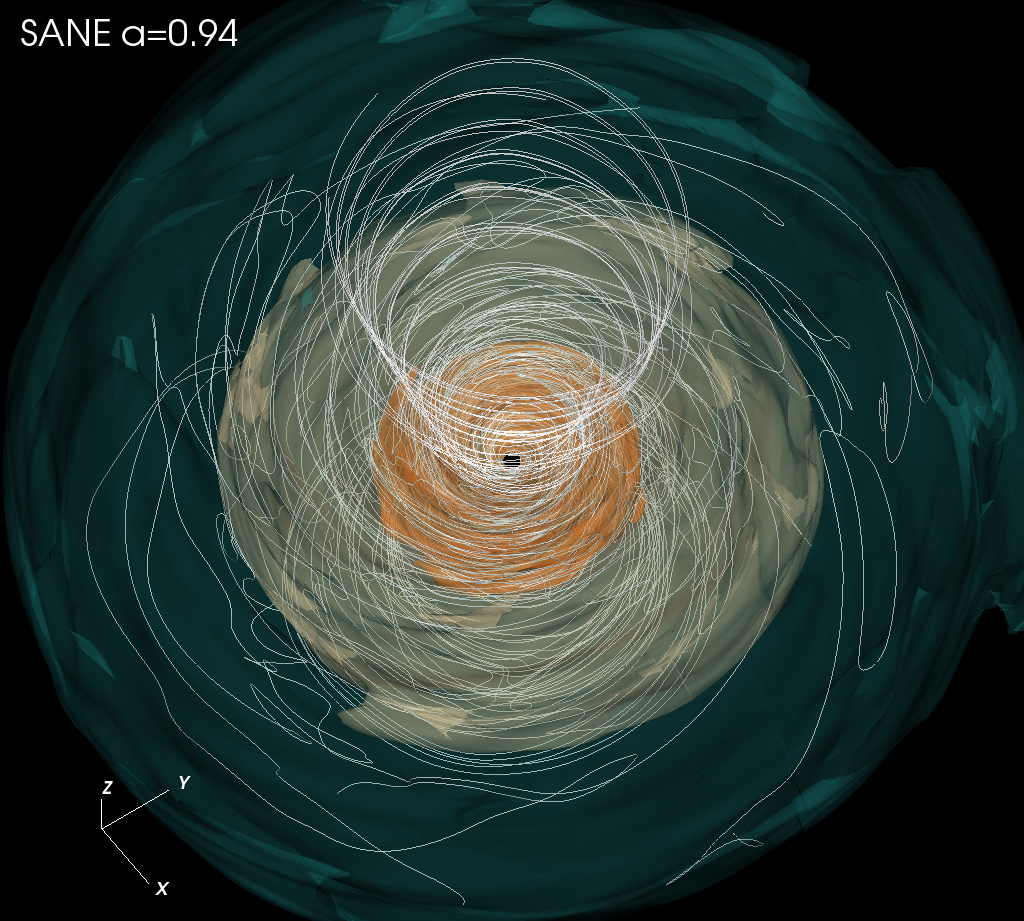
\includegraphics[width=0.425\textwidth]{figures/sane_3D_corrected.png}\hspace{1.5pt}%
  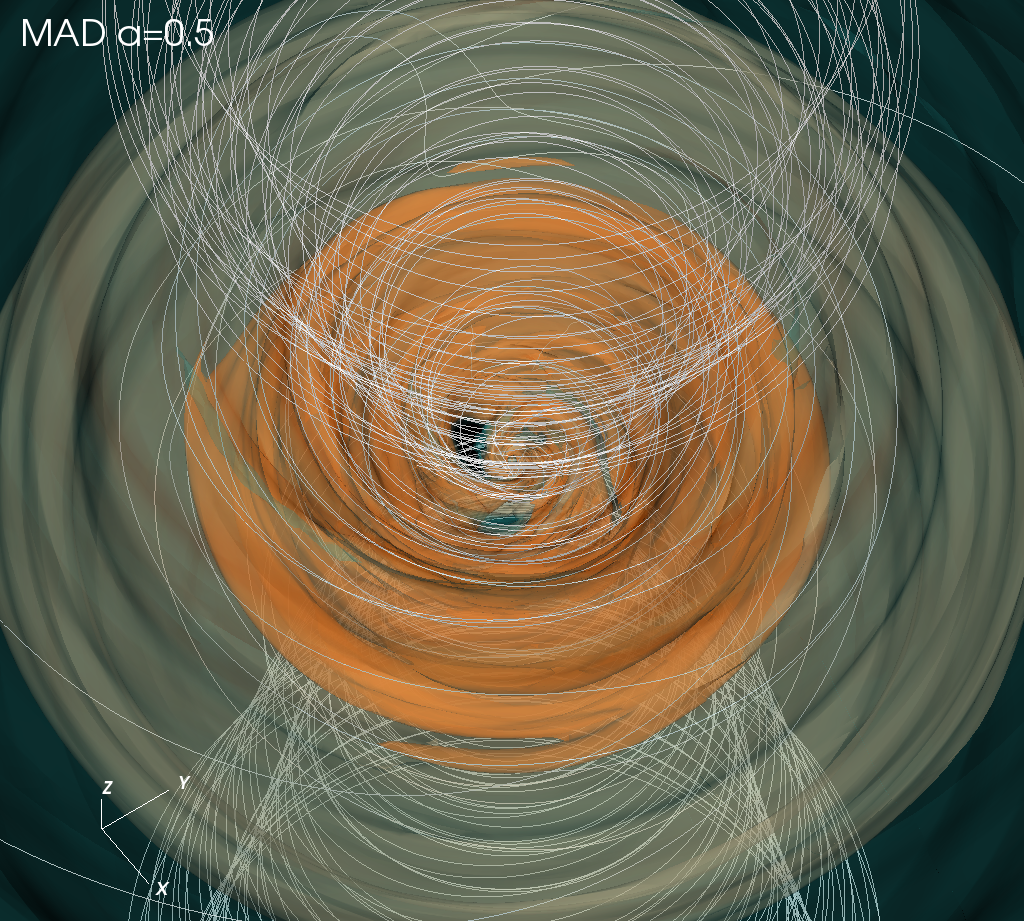
\includegraphics[width=0.425\textwidth]{figures/mad_3D_corrected.png}\\
  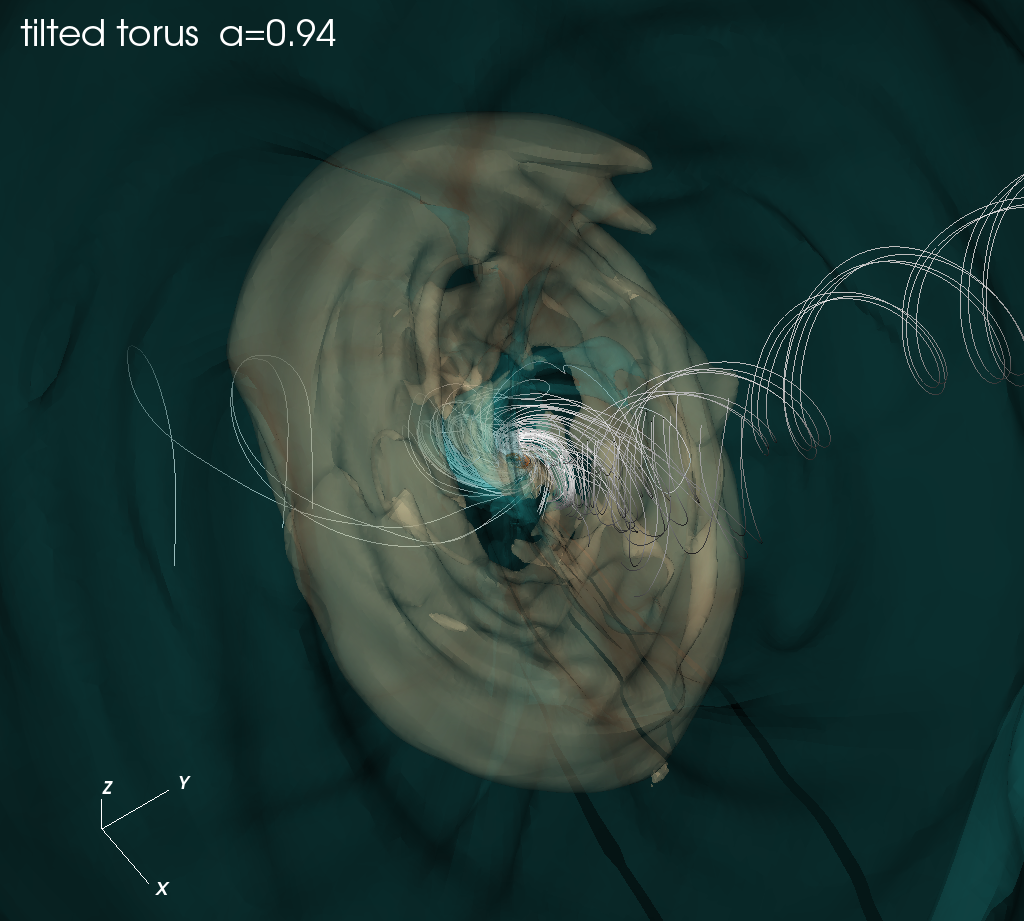
\includegraphics[width=0.425\textwidth]{figures/tilted_3D_corrected.png}\hspace{1.5pt}%
  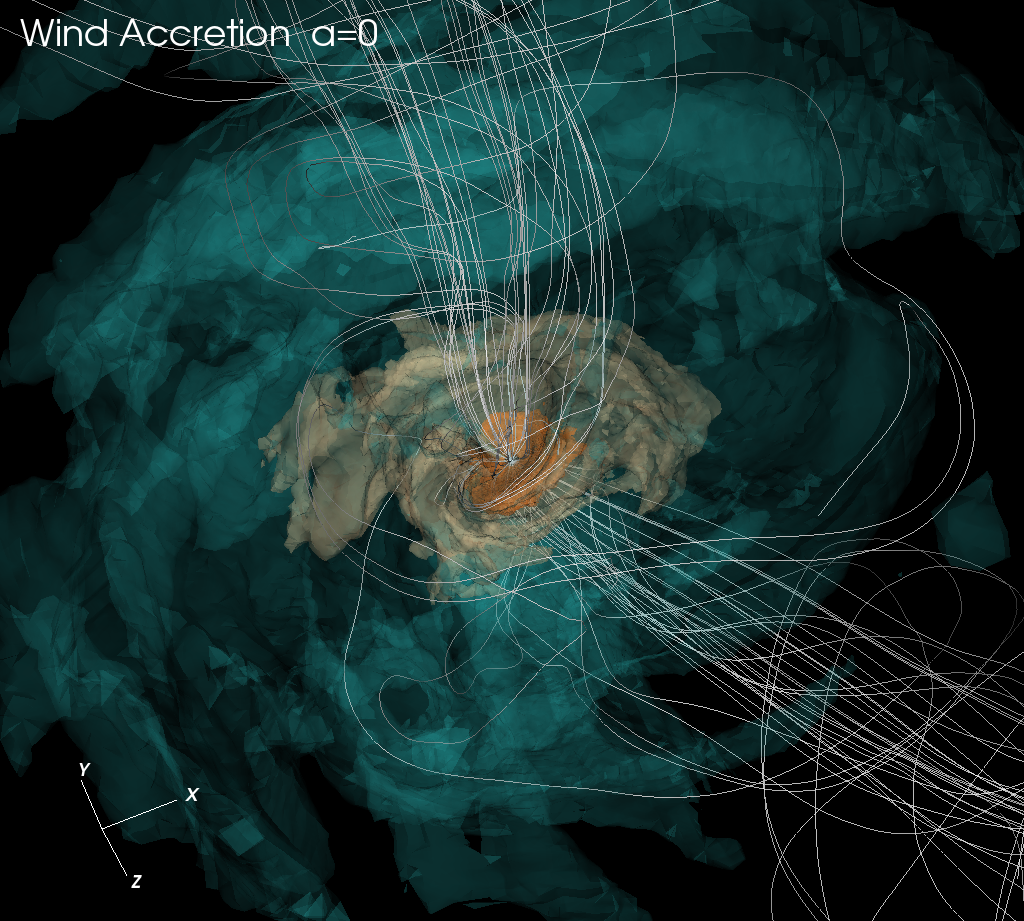
\includegraphics[width=0.425\textwidth]{figures/ressler_3D_corrected.png}
  \caption{3-D overview of selected GRMHD simulations of \sgra in our library.
    The color marks constant dimensionless density surfaces and lines follow magnetic field lines (the magnetic field lines shown are only those which are attached to the inner part of the accretion flow, at $r\approx 5~\rg$).
    Two top panels show accretion simulations with default torus initial condition and
    two bottom panels show non-standard accretion models. In case of spinning black holes, the spin is aligned with z-axis.}
  \label{fig:GRMHD}
\end{figure*}

One critical feature of the GRMHD simulations that is important for the interpretation of our results is the temperature profile.
Figure \ref{fig:grmhd_temp} shows the time- and azimuth-averaged profiles of the midplane dimensionless {\em ion} temperature in a set of aligned GRMHD simulations.
The temperature profiles exhibit strong trends with spin and magnetic state (MAD or SANE) that drives many of the trends seen in the radiative models: MAD models are factor of several hotter than than SANE models and both MAD and SANE become hotter as $\abh$ increases.

\begin{figure*}
  \centering
  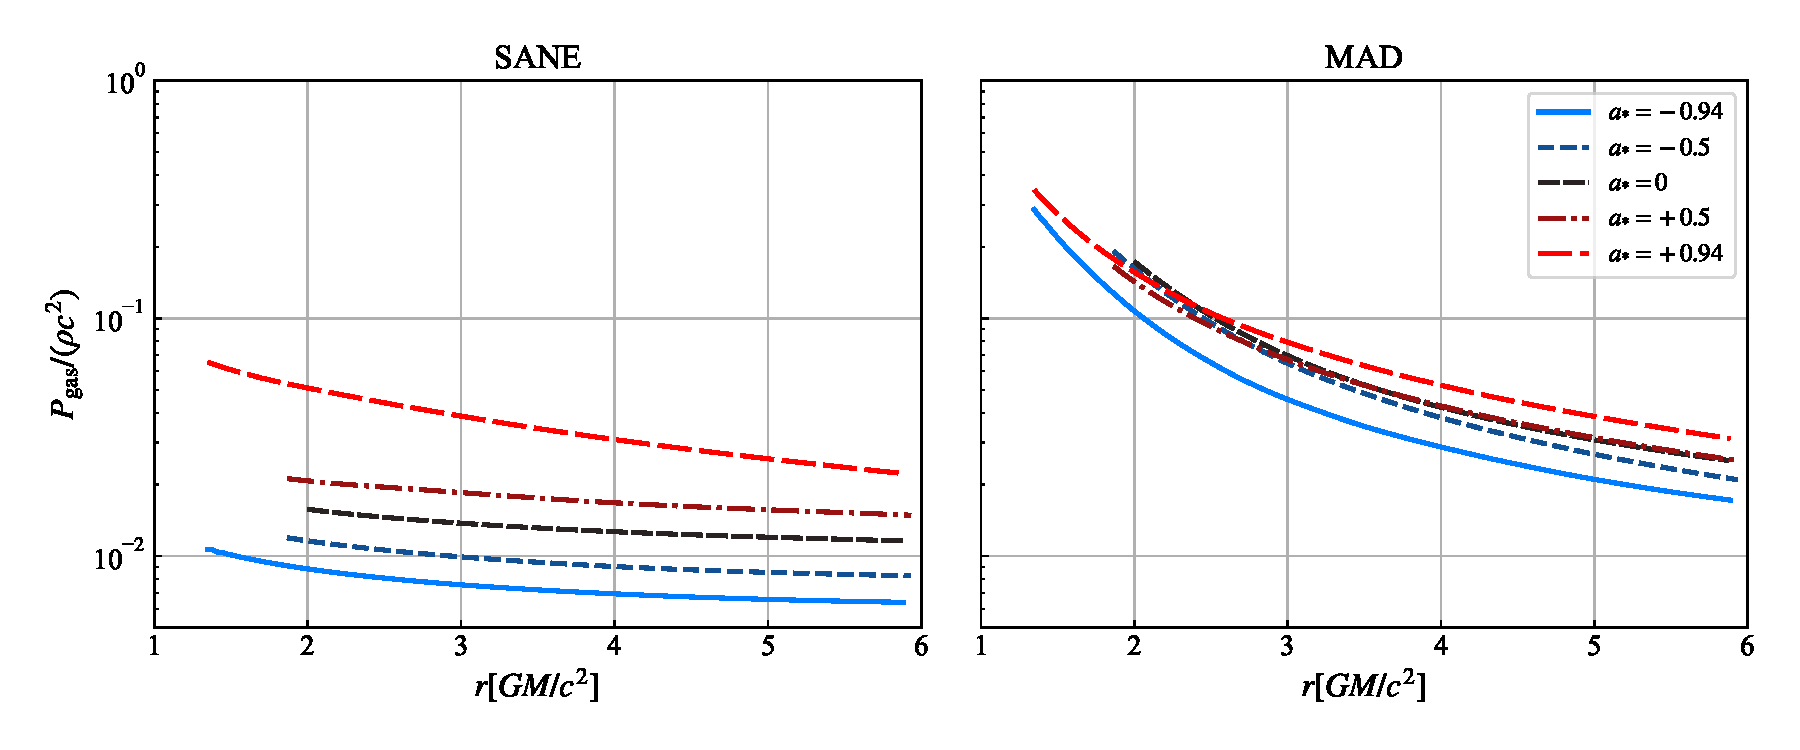
\includegraphics[width=0.9\textwidth]{figures/grmhd_temp.pdf}
  \caption{Time- and azimuth- averaged profiles of midplane dimensionless ion temperature in fiducial GRMHD simulations from \kharma.
    Evidently MAD models are hotter than SANE, and both MADs and SANEs grow hotter as the black hole spin $\abh$ increases.
    The hottest models are $\abh = 0.94$ MAD models.}
  \label{fig:grmhd_temp}
\end{figure*}

%------------------------------------------------------------------------------
\subsubsection{Radiative Transfer Model}

Synthetic images are generated from the GRMHD simulations in a radiative transfer step.
The transfer step requires:
\emph{i})~a model for the electron temperature and electron distribution function (hereafter eDF);
\emph{ii})~an assignment of a density scale to the GRMHD simulation;
\emph{iii})~a numerical radiative transfer step performed after the GRMHD simulation, assuming that the plasma evolution is unaffected by radiation.

The transfer step requires that we specify any parameters associated with the eDF (e.g. $\Rh$), the inclination $i$ (angle between the black hole spin axis and the line of sight), and an accretion rate or equivalently a density scale, which is not determined by the GRMHD simulation.

%..............................................................................
\subsubsubsection{Electron Distribution Function}
\label{sec:eDF}

In \emph{thermal} models electron energies are distributed into the Maxwell-J{\"u}ttner distribution function:
\begin{align}\label{eq:thermaleDF}
  \frac{1}{n_e}\frac{dn_e}{d\gamma} = \frac{\gamma^2 \sqrt{1-1/\gamma^2}} {\Theta_e K_2(1/\Theta_e)} \exp\left(-\frac{\gamma}{\Theta_e}\right);
\end{align}
where $K_2$ is the modified Bessel function of the second kind and $\gamma$ is the Lorentz factor of an electron. Recall $\Theta_e = k_b T_e/(m_e c^2)$, which is determined by the ion-electron temperature ratio $R \equiv T_i/T_e$:
\begin{align}\label{eq:te_vs_R}
  T_e=\frac{2 m_p u}{3 k_B \rho (2+R)}.
\end{align}
Here $u$ and $\rho$ are the internal energy density and rest-mass density from the GRMHD simulation, and we assume that the ions are nonrelativistic with adiabatic index is $5/3$ and the electrons are relativistic with  adiabatic index is $4/3$.
Thermal models are motivated by the idea that wave-particle scattering drives partial relaxation of the eDF, even though Coulomb scattering is ineffective.

The temperature ratio in a parcel of plasma depends on a balance between microphysical dissipation, radiative cooling, and fluid transport. Models for collisionless dissipation vary widely in their predictions for the ratio of heat deposited in ions and electrons, but most depend strongly on the local magnetic field strength. For simplicity, we adopt a prescription in which the temperature ratio is only a function of the plasma beta
This motivates a prescription in which the temperature ratio is a function of the plasma
$\beta \equiv P_\mathrm{gas}/P_\mathrm{mag}$ \citep{2015ApJ...799....1C}.
We adopt the same model as \citetalias{M87PaperV} and \citetalias{M87PaperVIII}, where $R$ is a smooth function adopted from \cite{2016A&A...586A..38M}:
\begin{equation}\label{eq:rhigh_prescription}
  R = \frac{T_i}{T_e} = \Rh \frac{b^2}{b^2+1} + \Rl \frac{1}{b^2+1}
\end{equation}
where $b \equiv \beta/\beta_\mathrm{crit}$.
This model has three free parameters: $\beta_\mathrm{crit}$, $\Rl$, $\Rh$.
We fix $\Rl = 1$ (consistent with the long cooling time in \sgra; see discussion in \citealt{M87PaperVIII}) and $\beta_\mathrm{crit} = 1$, but allow $\Rh$ to vary from 1 to 160.

In \emph{non-thermal} models, the eDF has a power-law tail extending to high energy.
We explore two implementations in this paper:
\emph{i}) a power-law distribution function
\begin{align}
  \frac{1}{n_e} \frac{d n_e}{d\gamma} &=
  \frac{p-1}{\gamma_{\min}^{1-p} - \gamma_{\vphantom{i}\max}^{1-p}}
  \gamma^{-p},
  \label{eq:nonthermaleDF}
\end{align}
which has power-law index $p$ and upper and lower limits $\gamma_{\min}$ and $\gamma_{\vphantom{i}\max}$; and
\emph{ii}) a so-called $\kappa$ distribution function, inspired by observations of the solar wind and by results of collisionless plasma simulations \citep[e.g.,][and references therein]{2015JPlPh..81e3201K}
\begin{align}
  \frac{1}{n_e} \frac{d n_e}{d\gamma} =
  \gamma \sqrt{\gamma^2-1} \left(1+\frac{\gamma+1}{\kappa w}\right)^{-(\kappa+1)},
  \label{eq:kappaeDF}
\end{align}
which has width parameter $w$ and power-law index parameter $\kappa$.

Evidently, any eDF assignment scheme is an approximation since the eDF depends in general on both local conditions and particle histories.
Notice that we also assume the eDF is isotropic and neglect electron-positron pairs.

Once the eDF is specified, the radiative transfer coefficients (emissivities, absorptivities, and rotativities) can be readily calculated; see \cite{2021ApJ...921...17M} for a recent summary.

%..............................................................................
\subsubsubsection{Model Scaling}

With the exception of the stellar wind-fed simulations, the GRMHD simulations considered in this work contain a characteristic speed, $c$, but are otherwise scale-free; they set $GM = c = 1$.
Physical scales are assigned during the radiative transfer step.
The black hole mass $\mbh$ fixes the length unit $\rg$ and time unit $\tg$.
Because the GRMHD simulations are non-selfgravitating, one is free to set a density scale, or equivalently the accretion rate $\dot{M}$ or plasma mass scale $\Munit$ \citep[see, e.g.,][for a full discussion]{Wong_2022}.

The plasma mass scale parameter $\Munit$ controls the plasma emissivity and the plasma optical depth and thus the source brightness.
We adjust $\Munit$ iteratively until the time-averaged 230\GHz flux densities of the models are within a few percent of the $2.4\,\mathrm{Jy}$ mean observed during the 2017 campaign (see next section).
Notice that, in this work, model parameters are always varied at constant time-averaged millimeter flux density.

%..............................................................................
\subsubsubsection{Radiative Transfer Calculation}

\begin{figure*}
  \centering
  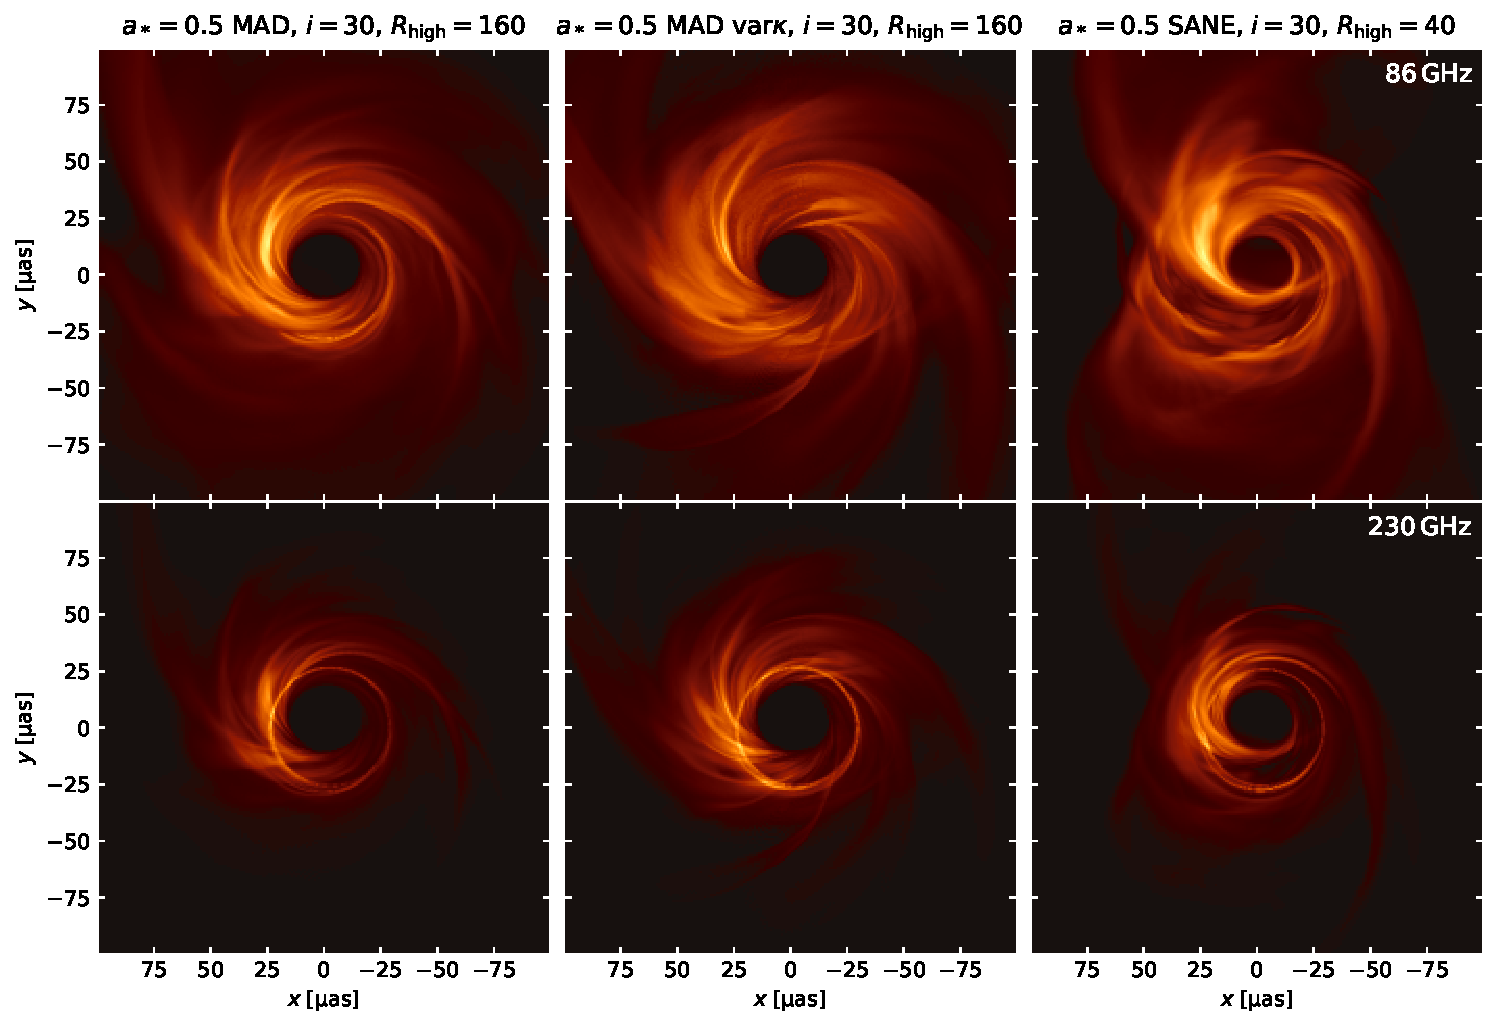
\includegraphics[width=\textwidth]{figures/example_imgs.pdf}
  \caption{Example models from the simulation library.
Left column: best-bet thermal MAD; middle column: nonthermal variable $\kappa$ MAD; right column: thermal SANE model.
Top row: 86\GHz images; bottom row: 230\GHz images.
Color represents intensity, or equivalently brightness temperature.
Angular momentum of the accretion flow projected onto the image points up.
These are relatively successful models satisfying most of the observational  constraints.}
  \label{fig:example_imgs}
\end{figure*}

\begin{figure*}
  \centering
  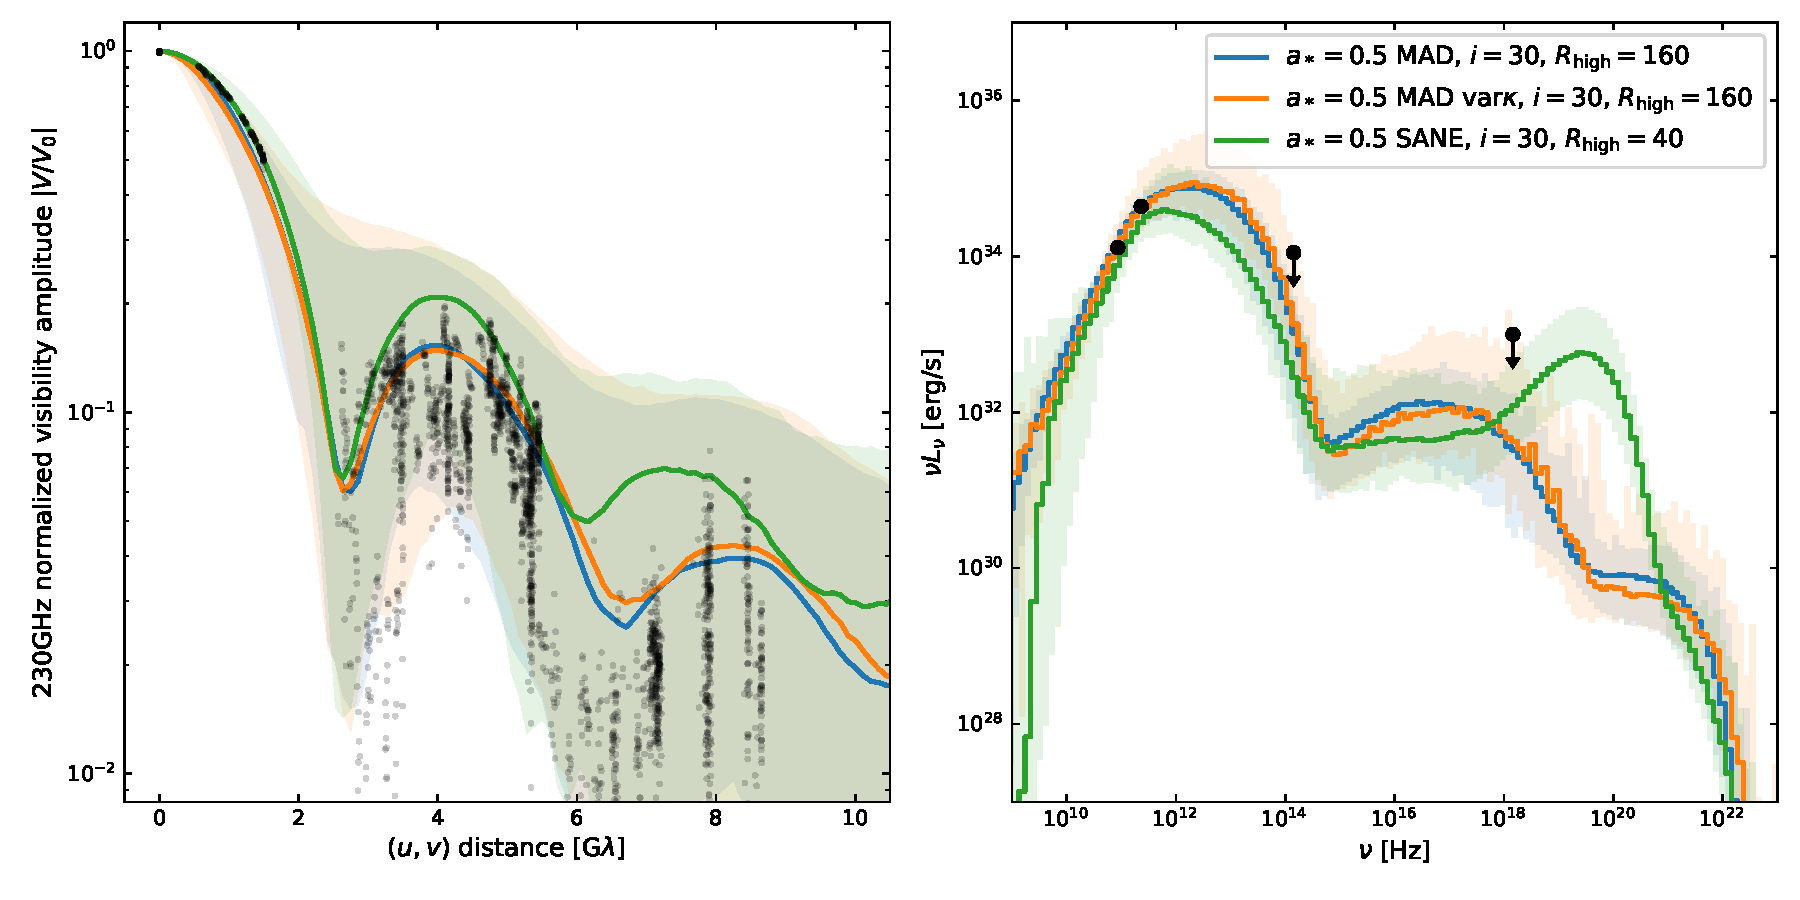
\includegraphics[width=\textwidth]{figures/example_vas_seds.pdf}
  \caption{Visibility amplitudes (left) and SEDs (right) of the three examples, compared with the calibrated EHT~2017 data.
Black symbols show observations.
Blue, orange, and green are the models shown in Figure~\ref{fig:example_imgs} (see also legend for details).
Observed VAs are 1\,minute incoherently averaged data from the HOPS pipeline on \aprilvii.
Model VAs are shown as a solid line for a section at position angle $0\degree$ for a single snapshot, and the band shows the 1st through 99th percentile over all position angles and all times; in this figure no noise is included in the model VAs.
Model SEDs show a solid line for the mean SED and a band for the range across snapshots.}
  \label{fig:example_vas_seds}
\end{figure*}

Given an eDF, density scale $\Munit$, the inclination $i$, and radiative transfer coefficients based on local properties of the plasma, the emergent radiation is obtained by integrating the radiative transfer equation.
We use two classes of numerical methods: observer-to-emitter ray tracing to generate synthetic images ({\tt ipole} scheme, \citealt{2018MNRAS.475...43M}, {\tt BHOSS} scheme, \citealt{2012A&A...545A..13Y}), and emitter-to-observer Monte Carlo to generate spectral energy distributions (SEDs, using {\tt grmonty} scheme, \citealt{2009ApJS..184..387D}).

All radiative transport calculations are carried out using the fast light approach, in which plasma variables are read from a single GRMHD dump file and are assumed not to change during ray tracing.
It has been demonstrated by \citet{2010ApJ...717.1092D} (and recently by \citealt{2021MNRAS.508.4282M}) that including light travel effects in the model introduces minor changes to light curves and images.
Further detail on numerical methods is given Appendix~\ref{app:radtrans}.
Comparisons of numerical methods \citep{2020ApJ...897..148G, Prather_et_al_2022} show that differences between radiative transfer schemes do not contribute substantially to the error budget.

The imaged are produced at 86\GHz, 230\GHz and 2.2\um (near infrared, hereafter NIR).
Direct imaging includes synchrotron and bremsstrahlung \citep[both ion-electron and electron-electron; see][for a recent review]{2020ApJ...898...50Y}.
The image library has a typical field of view (full width), resolution (pixel count), and half-width angular size of: $800\uas$, $200 \times 200$, $80 \vartheta_\mathrm{g}$ at 86\GHz; $200\uas$, $400 \times 400$, $20 \vartheta_\mathrm{g}$ at 230\GHz; and $100\uas$, $200\times 200$, $10 \vartheta_\mathrm{g}$ at $2.2\um$.
A few models are imaged with larger field of view or higher resolution.

The SEDs are produced for a set of narrow bins in inclination angle. At each inclination, the SED is averaged over azimuth.
The SED includes synchrotron, bremsstrahlung, \emph{and} Compton scattering.

We find that, although $2.2\um$ emission is usually dominated by synchrotron, occasionally $2.2\um$ synchrotron is so weak that Compton scattering dominates.
We also find that the X-ray can be dominated by either Compton scattering or bremsstrahlung, with the latter dominating in models with a large population of cold electrons at large radius.
Figures~\ref{fig:example_imgs} and \ref{fig:example_vas_seds} show examples of model images and multiwavelength SEDs from our library.

The GRMHD simulation-derived temperatures are unreliable in regions where $\sigma \equiv B^2/(8\pi\rho c^2)$ is large, because truncation error in integration of the total energy equation produces large fractional errors in temperature.
All our radiative transfer models therefore set the emissivity, absorptivity and inverse-Compton scattering cross-sections to $0$ at $\sigma > \sigma_\mathrm{cut} = 1$.

%==============================================================================
\subsection{Summary of \sgra Model Library}

%You can check which data is available here:
%https://docs.google.com/spreadsheets/d/1gw9ichvvYGHLFsZl2wlxqu-O03qEULrwcw3Wixd8BhQ/edit#gid=930351969
%not sure that gives complete answer, but it will help.

A summary of radiative transfer calculations is given in Table~\ref{tab:radiativemodels}. The entire image library contains $6$ simulation sets; thousands of points in model parameter space and $\sim 1.8$M images at each of 86\GHz, 230\GHz, and $2.2\mu$, and $\sim1.3$M SEDs.
The images and SEDs occupy about $50$TB.

We refer to the thermal, $\Rh$ models as ``fiducial'' models, and the remainder as ``exploratory'' models that test the effect of incorporating changes in the eDF or initial conditions.
Nearly all the exploratory models (exceptions are described in the discussion) are imaged over $5 \times 10^3 G M/c^3$, in comparison to $> 10^4 G M/c^3$ for the fiducial models. The sampling noise in the exploratory models is therefore larger than in the fiducial models and they cannot be tested as rigorously as the fiducial models.

The library contains multiple, redundant models for the fiducial models and variable $\kappa$ models.
This provide some control over uncertainties associated with variations in GRMHD simulation setup and algorithms.

\begin{deluxetable*}{ccccccc}\label{tab:radiativemodels}
\tablecaption{EHT Model Library}
\tablehead{
  \colhead{Simulation}               &%
  \colhead{Transfer Code}            &%
  \colhead{$\Rh$}                    &%
  \colhead{Inclination}              &%
  \colhead{SED}                      &%
  \colhead{$\Delta t/(10^4 GM/c^2)$} &%
  \colhead{Notes}%
  }
\startdata
\multicolumn{7}{c}{\bf Fiducial models}\\
\hline
\multicolumn{4}{l}{\it Thermal $\Rh$ models} & & &\\
\kharma& \ipole & 1, 10, 40, 160 &  10, 30, ..., 170 &  Yes & 15--30 & \\
\bhac  & \bhoss & 1, 10, 40, 160 &  10, 30, ..., 90  &  Yes & 20--30 & \\
\hamr  & \bhoss & 1, 40, 160     &  10, 50, 90       &  Yes & 20--35 & \\
\koral & \ipole & 20             &  10, 30, ..., 170 &  No  & 5--100 & \\
\hline
\multicolumn{7}{c}{\bf Exploratory models}\\
\hline
\multicolumn{4}{l}{\it Thermal $\Rh$ models} & &  &\\
\hamr Tilted   & \bhoss & 1, 40, 160 & 10, 50, 90 &  Yes & 100--103 & \\
Wind Accretion & \ipole & 13, 28     & N/A        &  No  & 10       &  \\
\hline
\multicolumn{4}{l}{\it Thermal critical $\beta$ model} & & & \\
\kharma & \ipole & N/A &  10, 50, 90 &  No & 30-35 &  \\
\hline
\multicolumn{4}{l}{\it Thermal + power-law models} & & & \\
\hamr &  \bhoss & 1, 40, 160 &  10, 50, 90 &  No & 30-35 & $p = 4$ \\
\hline
\multicolumn{4}{l}{\it Thermal + $\kappa$ models} & & & \\
\bhac & \bhoss & 1, 10, 40, 160 &  10, 30, ..., 90     &  No  & 25-30 & $\kappa = 5$ \\
\bhac & \bhoss & 1, 10, 40, 160 &  10, 30, ..., 90     &  No  & 25-30 & $\kappa = 3.5 (\epsilon_0 = 0.05)$\\
\bhac & \bhoss & 1, 10, 40, 160 &  10, 30, ..., 90     &  No  & 25-30 & $\kappa = 3.5 (\epsilon_0=0.10)$ \\
\bhac & \bhoss & 1, 10, 40, 160 &  10, 30, ..., 90     &  No  & 25-30 & $\kappa = 3.5 (\epsilon_0=0.20)$ \\
\bhac & \bhoss & 1, 10, 40, 80, 160 &  10, 30, ..., 90 &  No  & 25-30 & variable $\kappa=\kappa(\beta, \sigma)$ \\
\hamr & \ipole & 1, 10, 40, 160 &  10, 30, ..., 90     &  Yes & 30-35 & variable $\kappa=\kappa(\beta, \sigma)$ \\
\enddata
\tablecomments{%
  Summary of the EHT \sgra model library. All models are imaged at $86\GHz$, $230\GHz$, and $2.2\um$ and some (see column 5) also have spectral energy distributions.
  For the wind-fed accretion model the viewing angle is set by the stellar orbits and $\Rh$ is set so the model matches the observed 230\GHz flux; $\Rh = 13, 28$ for models with stellar wind magnetizations $\beta = A, B$, respectively \cite{2020ApJ...896L...6R}.
}

\end{deluxetable*}


\section{Observational Constraints}\label{sec:observations}

\sgra is one of the most observed objects in the sky.  It has been observed with a slew of telescopes, across 5 decades in time and more than 17 decades in frequency. We need to select a manageable subset of this data to constrain our models. In doing so we have attempted to select
\emph{i})~approximately uncorrelated constraints, so that each tests a distinct aspect of the model;
\emph{ii})~constraints based on data that can be simulated with the models; and
\emph{iii})~constraints based on EHT 2017 1.3\mm VLBI data or based on photons produced within or close to the 1.3\mm emission region that are contemporaneous or near-contemporaneous.

Variability complicates the comparison of \sgra models to the data. Even an ideal evolution of a successful model will never match the data point for point because the space of possible realizations of the model is large; the dataset is high dimensional.  We expect the {\em distribution} of  observables derived from a successful model to match the data, however, if the model is run long enough to sample the distribution.  For example, the distribution of the 86\GHz flux density $F_{86}$ for a model ought to contain the observed $F_{86}$.

Most observables are correlated over $\tau\sim$ few $\times 100 \tg$.  To obtain the mean and variance of the model distribution to accuracy $f$ from a GRMHD model, then, requires running it for $\sim \tau/f^2 \sim 30,000 (\tau/300) (f/0.1)^{-2}$, assuming the model decorrelates completely at intervals $\gg \tau$.  A GRMHD model of duration $30,000 \tg$  costs $10^3-10^4$ node-hours, depending on resolution, code, and hardware.  This is expensive since $\sim 10$ runs are used for each model set, and runs need to be repeated for multiple values of numerical parameters (e.g. resolution).  Most of our models are run for $30,000 \tg$; a few are run to $100,000 \tg$.  The model distributions therefore contain sampling noise, and this must be accounted for in model selection.  For some  constraints (e.g. m-ring fits; see below) this can be done by sampling the model at a cadence similar to the correlation time and then using a 2-sample KS test to compare the observed and model distributions.

%==============================================================================
% \subsection{Scattering Models}

%==============================================================================
\subsection{EHT Observational Constraints}

%\ckc{ck's first pass}
%\mw{I think it would be good to mention the EHT array composition (name the telescopes)}
%\cfg{much of this material could be incorporated by reference to paperII}

% CFG: suggest we can do without these.  They do make what we are doing clearer, but it is yet another figure in a bazillion-figure paper.
%\begin{figure*}
%  \centering
%  \includegraphics[width=0.5\textwidth]{figures/va_comparison.pdf}%
%% \note{altex: (left) visibility amplitude vs baseline for the day(s) that
 %   this study use, overplotted by the visibility amplitude from a
%    fiducial model.
%    Similar to paper~II, figure~7.
%    Visually mark null location constraint, pre-imaging size (i.e.,
%    second moment).
 %   (right) SED from Gurther overplotted by the SEDs from a fiducial
%    model.
%    Visually mark the SED constraints.}
%  \caption{(\emph{left}) Measured correlated flux densities of \sgra
 %   on April 7, 2017, from the HOPS pipeline, overplotted with a fiducial
%    GRMHD+GRRT model.
%    Details on the data can be found in paper~II, section~5.
%    A description of the fiducial model is in section~\ref{sec:models}.
%    (\emph{right}) \ckc{Q: do we want to show only EHT observation and
 %     referencing to other papers for non-EHT constraints?
%      Or should we have representative figures for all measurements?}}
%  \label{fig:visibility}
%\end{figure*}

%The EHT observed \sgra at 1.3 mm during the 2017 April 5--11 observing campaign and obtained horizon scale complex visibilities.  Figure~\ref{fig:visibility} shows the visibility amplitudes on April 6 and 7 from  the HOPS pipeline, overplotted with visibility amplitudes derived from a model.  Evidently there are nulls near $\sim 5\,\mathrm{G}\lambda$ and $7\,\mathrm{G}\lambda$, suggesting a ringlike structure.

We test the models against EHT interferometric data in three ways.
First, we check the location of the first minimum in the visibility amplitudes and the value of the visibility amplitudes on long baselines (``null constraint'').
Second, we compare an estimate of the source size (``second moment constraint'') to an estimate from short baselines.
Finally, using a variant of a procedure from \citetalias{PaperIV}, we compare fits for the diameter, width, and asymmetry of an m-ring (a parameterized image-plane model) to the GRMHD models.

%------------------------------------------------------------------------------
\subsubsection{230\GHz VLBI Null Location}

Our first constraint provides a simple morphological check on the visibility amplitudes.
We ask two questions of each model snapshot: is the first minimum in the visibilities in about the right place,
and are the long-baseline visibility amplitudes comparable to the data?
For comparison, we use data from \aprilvii, which has the best $u$-$v$ coverage near minima in the visibility amplitudes.

The minima locations and long-baseline amplitudes are sensitive to the source structure.
For example if the source is a simple, circularly symmetric ring of finite width then the location of the first minimum depends only on the ring diameter, while the visibility amplitude on long baselines depends mainly on ring width.
GRMHD models are more complicated, with significant structural fluctuations.
The minima locations and depths, and long-baseline amplitudes, are expected to fluctuate (e.g., \citealt{2018ApJ...856..163M} and \citetalias{M87PaperV}).

For the ``null location'', the first visibility minimum in both the N-S and E-W directions occurs between 2.5--3.5\,G$\lambda$ in the data.
We do not consider the depth of the null in this simple check.

\cfg{best references for scattering?}
For the ``long baseline'' interval between 6--8\,G$\lambda$, the visibility amplitude has $\lesssim 4\%$ of the zero-baseline flux, always.
One complication when comparing models to data on long baselines is the effect of interstellar scattering.
Diffractive scattering effectively convolves the image with a smooth kernel and can reduce the amplitudes to about $\sim 50\%$ of their unscattered values in the 6--8\,G$\lambda$ range (ref!!).
Refractive scattering, on the other hand, introduces noise at all baselines of order 0.5--3\%, depending on the particular characteristics of the scattering screen (ref).  To account for these effects, we classify a model snapshot with $|V|$ in this range that is $< 5\%$ of the zero baseline flux as compliant.

To apply this constraint, we compute the visibility amplitudes $V$ of each model snapshot along position angles $0^\degree$, $45^\degree$, $90^\degree$, $135^\degree$.  We find the first minimum numerically and compute the median visibility amplitude between 6 and 8\,G$\lambda$.
We classify a snapshot as compliant if \emph{i}) for at least one position angle the first minimum falls between 2.5 and 3.5\,G$\lambda$ and \emph{ii}) at no position angle does the median visibility amplitude exceed $(0.04 / 0.5) V_0$.

We evaluate the fraction of snapshots from each model that are compliant using the criteria described above.  We reject models with compliance fraction $< 1\%$.

%------------------------------------------------------------------------------
\subsubsection{230\GHz VLBI Pre-Image Size}

%\ckc{ck's first pass}
%\cfg{edited on 2 dec}

The source size can be characterized using the second moments of the source image on the sky.  The second moments in the image domain map to second derivatives of the visibilities near zero baseline in the $uv$ domain, so short baseline visibility amplitudes can be used to directly estimate the source size.

%The second moment of an EHT source corresponds, in the $(u,v)$ domain, to
%the second derivative of the visibility amplitude near zero baseline length.
%That is, the 2nd moment tensor
%\begin{equation}
%    \sigma_{ij} \equiv \int \, d^2x\, x_i x_j I/\int \, d^2x \, I = (2\pi)^2 %\left(\partial_i \partial_j \tilde{I}\right)/\tilde{I}
%\end{equation}
%where $I$ is the intensity, $\tilde{I}$ its Fourier transform, $i =
%x,y$ on the left and $i = u,v$ on the right, and the terms on the
%right are evaluated at $u = v = 0$.
%Depending on the structure of the visilbiity amplitudes, a pair of visibility amplitudes ($|\tilde{I}|$) on short baselines or
%the zero baseline flux can therefore be used to estimate the second moments of the image.

\cfg{is this scattered or unscattered?}

This procedure is used in EHT3 \citetalias{PaperIII} to set an upper limit of 95\uas FWHM on the second moment and lower limit of 38\uas on the second moment along a particular directions through the source, with the direction determined by the orientation of the short baselines.  This is done without any assumption about the structure of the source; if we used a ring prior the constraint would be narrower.

To assess a model we evaluate, for each synthetic 230\GHz image, the second moment tensor and find its eigenvalues $\lambda_\mathrm{maj}^2/(8\log 2)$ and $\lambda_\mathrm{min}^2/(8\log 2)$, where $\lambda_\mathrm{maj}$ and $\lambda_\mathrm{min}$ are the FWHM of the major and minor axis.  The image is deemed compliant if it is consistent with the data for any orientation, that is, if $\lambda_\mathrm{maj} > 38\uas$ \emph{or} $\lambda_\mathrm{min} < 95\uas$.  We reject models with a compliance fraction $< 0.01$.

\ckc{I suggest we move the 2nd moment first, then null location, then m-ring.
  The reason is that the wide (unconstraining) 2nd moment is caused by allowing it to be just a Guassian (i.e., ignore the minima).
  We then tighten the constraint by regonizing there's a minima using the null analysis.  And then do the fit.}

%------------------------------------------------------------------------------
\subsubsection{230\GHz M-Ring Fitting}

How can we extract information about the spatial structure of the source from noisy, fluctuating data with limited UV coverage, and compare that to noisy, fluctuating models?
Our strategy is to fit a source-plane model to the data and summarize the source structure using the distribution of fit parameters.

\citetalias{PaperIV} fits an ``m-ring'' source model to the April~7 data.  Here we use a simplified m-ring model: a $\delta$ function in radius with diameter $d$ multiplied by a truncated (up to $m = 3$) Fourier series, convolved with a Gaussian of width $w$.  In addition the model contains a centered Gaussian component, with amplitude and width as free parameters, to absorb large scale emission and emission interior to the ring.

The simplified m-ring model has 10 parameters; 3 are well constrained and physically interpretable and are therefore used here: the m-ring diameter $d$, the m-ring width $w$ (FWHM of the convolving  Gaussian), and the $m=1$ relative amplitude $\beta_1$.

We fit the m-ring independently to ``snapshots'' consisting of 2-minute intervals of EHT data. Over these short intervals, we approximate the source to be static.  Uncertainties in the fitted m-ring parameters are dominated by the limited baseline coverage during these snapshots rather than by calibration uncertainties or thermal noise. Because snapshots that are close in time sample nearly identical baselines, they do not provide additional model constraints.

Thus, to compare fitted m-ring parameters from the EHT data to those for synthetic data from simulations, we focus on a reduced comparison dataset that consists of only a subset of scans with the best baseline coverage. We select scans that are widely separated in time, so that they sample distinct baseline coverage. For the comparison dataset we selected ten 120-\sec scans spread approximately uniformly through EHT observations on \aprilvii.  They are separated by an average of $\simeq 1240\sec \simeq 60 \tg$, which is small compared to the visibility amplitude correlation time in the models (see Georgiev et al. 2022). The scans were selected to have > 10 baselines, and integration time at all stations $> 40s$.    Only modest changes in model selection were observed if any one scan was removed from the comparison.  The data were de-scattered before fitting, that is, the visibility amplitudes were divided by the scattering kernel.  Maximum likelihood m-ring parameters were found for each scan.

The maximum likelihood m-ring parameters are listed in Table~\ref{tab:mringfits}.  Evidently the fit parameters are noisy.  The fit for $d$ range from 39\uas to 84\uas, for $w$ from 9\uas to 21\uas, and for $\beta_1$ from $0.04$ to $0.48$ (we require $\beta_1 \le 0.5$ to guarantee  positivity of the model image).

\begin{deluxetable}{ccccc}
\tablecaption{M-Ring Fits to EHT Observations}
\tablehead{ %
\colhead{Scan \#} & %
\colhead{t [UTC hrs]} & %
\colhead{d [$\mu$as]} & %
\colhead{w [$\mu$as] } & %
\colhead{$\beta_1$} %
}
\startdata
111 & 11.28 & 83.87 & 8.87  & 0.122 \\
121 & 11.78 & 57.09 & 13.98 & 0.220 \\
125 & 11.92 & 55.63 & 16.46 & 0.132 \\
130 & 12.35 & 40.68 & 19.08 & 0.039 \\
134 & 12.62 & 57.22 & 17.22 & 0.368 \\
142 & 12.92 & 58.80 & 17.55 & 0.208 \\
149 & 13.28 & 52.31 & 21.16 & 0.278 \\
155 & 13.75 & 38.94 & 18.17 & 0.482 \\
163 & 14.05 & 56.22 & 19.86 & 0.470 \\
171 & 14.38 & 39.48 & 17.71 & 0.408 \\
\enddata
\end{deluxetable}
\label{tab:mringfits}

The variation in fit parameters could be caused by source variability, thermal noise, and gain variations.  In the models the main driver of fit variations is source variability.

Next, we read in a series of model images, generate synthetic data for each image for each scan at four assumed position angles for the image, and fit m-rings to the synthetic data.  This produces a distribution of m-ring parameters for each model.

The synthetic data is generated as follows.  A model image $I(x,y)$ is fourier transformed to complex visibilities $V(u,v)$ with an assumed position angle, then sampled on baselines $i$ drawn from the comparison scan, $V_i \equiv V(u_i,v_i)$.  Normally distributed thermal noise $\delta V_{th,i}$ with amplitude based on telescope performance during the scan is added, and multiplicative, normally distributed noise with unit variance $N$ is added to crudely model gain corrections: $\tilde{V}_i = V_i (1 + \epsilon N) + \delta V_{th,i}$.  We set $\epsilon = 0.05$, but no significant changes in fit parameters were observed for $\epsilon = 0.02$.  We then fit to the visibility amplitudes $|\tilde{V}_i|$ and closure phases.
%arg$(\tilde{V}_i \tilde{V}_j \tilde{V}_k^*)$, where $ijk$ form a triangle in the $(u,v)$ plane.
The procedure was repeated for 4 positions angles (orientations of the image on the sky) and for model images separated by $500 \tg$ (comparable to a correlation time; no significant changes were observed if more position angles were used).  This results in, for example, a sample of $30$ fits per scan per position angle for the Illinois thermal model set, or a total of $30 \times 10 = 300$ samples in each distribution.

In comparing the models to the data we
\emph{i}) generate the distribution of fit parameters at each position angle;
\emph{ii}) use a Kolmogorov-Smirnov test to compare the distribution of $300$ synthetic data fits with the distribution of $10$ observational fits, and obtain a p-value (what is the probability they are drawn from the same underlying distribution?);
\emph{iii}) average p-values over position angles (i.e. marginalize over position angle; the models do not show a significant position angle preference); and
\emph{iv}) reject the model if $p < 0.01$.

%==============================================================================
\subsection{Non-EHT Constraints}

In addition to the EHT data, the SED of \sgra is well constrained \citetalias{PaperII} and thus potentially useful for model selection.
We limit comparison to three bands: 86\GHz, 2.2\um, and x-ray.

%------------------------------------------------------------------------------
\subsubsection{86\GHz Flux}

The Global Millimeter VLBI Array (GMVA) observed \sgra on April 3, 2017, just 3 days ($\approx 13,000 \tg$) before the EHT campaign.
\citet{2019ApJ...871...30I} estimate that the compact flux is $F_{86}=2.0 \pm 0.2\,\mathrm{Jy}$ ($2\sigma$ errors; S. Issaoun, private communication).

We compute a library of 86\GHz images for all GRMHD snapshots for all models, and from that the 86\GHz flux density $F_{86}$.  We assume normally distributed measurement errors with $\sigma = 0.1\,\mathrm{Jy}$, and convolve the $F_{86}$ distribution for each model with the resulting Gaussian.  We reject models with CDF $< 1\%$ or $> 99\%$ at $2.0\,\mathrm{Jy}$.

%------------------------------------------------------------------------------
\subsubsection{86\GHz Image Size}

The GMVA observations from April 3, 2017 constrain the FWHM of the source major axis ${\rm FWHM}_{maj} = 146^{+11}_{-12}\uas$ \citep[95\% confidence][]{2021ApJ...915...99I}.

We compute the major axis FWHM for each image in the 86\GHz image library.  We assume normally distributed errors with $\sigma = 6\uas$, and convolve the model major axis distribution with the normal distribution.  We reject models with CDF $< 1\%$ or $> 99\%$ at $146\uas$.

Our synthetic 86\GHz images have a 800\uas field of view.  A 200\uas field of view cuts off enough emission that the major axis is biased downward in many models by $\sim 20\%$.  Increasing the field of view beyond 800\uas has negligible effect.

%------------------------------------------------------------------------------
\subsubsection{NIR (Non-Overproduction) Constraints}\label{subsec:nir}

\cfg{need citation for flare rate}

\sgra flares in the near infrared (NIR; 2.2\um) a few times per day (1 day is $\simeq 4200 \tg$), and has a quiescent flux that in 2017 was estimated to be $\simeq 1.0$mJy \citep{2020A&A...638A...2G}.  Since there is as yet no generally accepted model for NIR flares we accept models that do not produce flares.  Our working hypothesis is that these models can be saved by perturbatively introducing a process that accelerates a small fraction of electrons into a nonthermal, NIR-bright tail.  If the model overproduces NIR with just the thermal electron population then we reject it.

We compute the 2.2\um flux density using one of two procedures.  If a full SED\textemdash which includes Compton scattering\textemdash is available, then it is used. The SEDs are generated by the \grmonty Monte Carlo code \citep[][also Wong et al. 2022, Davelaar et al. 2022]{2009ApJS..184..387D}. If a full SED is not available then we compute a NIR image that includes only synchrotron emission and absorption (although synchrotron absorption is negligible in the NIR for \sgra).  We reject the model if the median NIR flux density exceeds $1.0\,\mathrm{mJy}$.

%------------------------------------------------------------------------------
\subsubsection{X-ray (Non-Overproduction) Constraints}

\cfg{need citation for flare rate}

\sgra flares in the X-ray less than about once per day.  Chandra observations during the 2017 campaign suggest an upper limit on the median (quiescent) $\nu L_\nu$ at $6$keV of $10^{33}\ergsps$ \citep{PaperIII}.

Similar to section \ref{subsec:nir}, we estimate $\nu L_\nu (6 {\rm keV})$ in two ways.  The SED is used if the model contains Compton scattering and bremsstrahlung.  If the SED is not available then we compute an X-ray image that includes only bremsstrahlung (which dominates the X-ray emission in thermal SANE models with $\Rh = 40, 160$) permitting us to eliminate a few additional models.  We reject the model if the median $\nu L_\nu(6\,\mathrm{keV}) > 10^{33}\ergsps$.

%==============================================================================
\subsection{Variability}

% * we can model ``long-term climate'' well but not ``long-term weather''.
% * Hence we only compare the slowly varying quantities such as mean/median 2nd moments (climate) but not modulation index (weather).
% * TODO: look up correct statistical terminology in weather/climate modeling and build that this into this paper.
% * Use review: https://agupubs.onlinelibrary.wiley.com/doi/full/10.1029/2019EA000586 , https://ui.adsabs.harvard.edu/abs/1993RvMP...65.1331A/abstract
%
% * multi-time scale
% * feeding at large and slow scale
% * time scale much shorter when the plasma reach horizon
% * at 1.3mm, we only see the flow near the horizon
% * a "hidden variable" problem that there're slowly varying "boundary conditions" that control the nature of the accretion flow
% * but we only see the fast varying flow
% * Given the boundary conditions (environment), GRMHD + GRRT is very successfully in predicting the time average images.  (Refer to consistent checks in appendex)
% * At the short time scale, the system is chaotic and sensittive to initial conditions.
% * We reach order-of-magnitude agreement.  But in terms of constraint they should not be used.
% * For the date we use, EHT observations show lower variability compared to what we expected.

%\cfg{I think we should just describe the observations here.}
%\ckc{We don't have a discussion section on variability yet.  Maybe under 5.7 or 5.8?}

\sgra shows variability on a wide range of timescales.  This is expected: fluctuations in stellar wind feeding at the scale of the S-stars plausibly introduce long timescale variations, while turbulence at smaller radii, down to the scale of the event horizon, plausibly introduce a spectrum of shorter timescale variations.  Quantitative comparison of observed variability to the models is therefore a potentially powerful tool for model selection.

Here we consider two measures of variability: one that characterizes variability of 230\GHz flux density in the light curves \citep{Wielgus2022} and a second that characterizes variability of the visibility amplitudes in EHT data \citep{PaperIV, NoiseModeling}.

We will find that $> 90\%$ of models fail the combined variability tests: the data is quieter than the models.  This is the most severe downselect of all our constraints. Given the noisy nature of the model selection process we do not interpret this as success for the surviving $10\%$, all of which fail other constraints.  Instead we interpret this as a particular and interesting failure of the entire class of GRMHD models to reproduce the observed variability.  We discuss possible reasons for this {\em variability crisis} in Section~\ref{sec:discussion}.

%The remaining non-variability constraints are still informative about the structure of \sgra.  We therefore set aside the variability tests and perform a final model selection considering only the remaining constraints.  This is a dangerous game in the sense that variability is deeply embedded in many of the remaining constraints (it determines the width of many of the model distributions that we use for selection, for example).  Still, it is remarkable that so many models look as much like the data as they do, and rather than set aside that information we use it to identify a final set of best-bet models.

%Although we provide a full discussion of model variability, we will not use it for model selection, under the notion that the variability is a higher-order - and therefore less well predicted -  feature of the models while lower order features, such as 86GHz flux density and 230GHz source geometry, are still well predicted.  This hypothesis can only be tested once models that accurately predicted variability are available.

%Compared to other astrophysical systems, optically thin black hole accretion systems such as \sgra are expected to show variabilities in a wide range of time scales, from the boundary conditions at the Bondi radius determined by the ``environment'', all the way to the turbulent fluctuations near the event horizon, or even plasma instability driven phenomena.
%Even excluding flares and detailed plasma physics, observations have shown intrinsic variability in \sgra~\citep{sgra lightcurve papers}.
%The standard theoretical interpretation is that the turbulence in the accretion flow drives the fluctuations in, e.g., temperature and magnetic fields, which then drive the fluctuations in the electromagnetic signals.
%Assuming that the magnetorotational instability (MRI) is the driving mechanism, the turbulence integrated time scale is simply the orbital time scale.
%Given that synchrotron radiation mainly comes from the inner accretion disk, this time scale is of order of 10 minutes.
%However, the chaotic nature of turbulence makes these short time scale variability difficult to predict.
%Therefore, we will not rule out models using short time scale variability.
%On the other hand, numerical simulations are very successful in predicting the slowly varying mean images, SEDs, etc because these are controlled by the conservation laws and the boundary conditions.
%This justifies the usage of mean and median quantities to constraint models described in the earlier sections.

%------------------------------------------------------------------------------
\subsubsection{ALMA Light curves}

%\mw{I edited this a bit}
% thanks Maciek -CG

ALMA and SMA produced \sgra light curves at 230GHz as a byproduct of the 2017 EHT VLBI observing campaign. The complete set of light curves is presented and analyzed in \cite{Wielgus2022}.

We have chosen to compare the models to the 7 April 2017 ALMA light using the 3 hour {\em modulation index} $\mi{3}$, where $\mi{T} \equiv \sigma_T/\mu_T$, $\sigma_T$ is the standard deviation measured over some interval $T$, and $\mu_T$ is the mean measured over the same interval.  We use $\mi{T}$ following \citet{2015ApJ...812..103C} because it is easy to describe, easy to compute, commonly used in the literature (in the X-ray astronomy literature it is ``rms \%''), and closely related to the structure function, since the expectation value for $\sigma_T^2$ is given by an integral over the structure function (see Lee et al. 2022).

We use $T = 3$ hours because it is comparable to the correlation time for $F_{230}$ in most of the models, and because it is similar to the characteristic timescales measured in damped random walk fits to the ALMA lightcurve \citep[see Table 10 of][]{Wielgus2022}.  Although the correlation times tend to be slightly longer than $3$hr, that is the longest timescale for which we can consistently estimate the mean and variance of the distribution of $\mi{3}$ from the models (accurate estimation for larger $T$ would require longer GRMHD integration times).  In a damped random walk process one can show that $\mi{3}$ is minimally correlated over consecutive 3 hour intervals (Lee et al. 2022).

We measure $\mi{3}$ in maximally spaced intervals in the ALMA lightcurve on April 6, 7, and 11.\footnote{The model comparisons are insensitive to interval spacing.}  We have also measured $\mi{3}$ in historical data for \sgra from 2005-2017 light curves.  The April 6, 7, and 11 values for $\mi{3}$ (5 in all: 0.029, 0.031, 0.051, 0.041, 0.099) are consistent with having been drawn from the historical distribution, although April 7 is among the quietest intervals on record and April 11 is one of the most variable intervals on record.

For each model we evaluate a light curve and use that to generate a distribution of $\mi{3}$.  We then use a KS test to ask whether that distribution is consistent with the historical distribution.
%The constraint comes from $M_T$ measured over 3 maximally spaced intervals
%in the 7 April 2017 ALMA light curve, where $M_3 = 0.024, 0.051,
%0.047$ (Wielgus et al. 2021). These values are consistent with being drawn from the distribution estimated from historical non-EHT 2005-2017 light curves.
%curves. \mw{maybe sth like "from the estimated distribution of the historical 2005-2017 lightcurves"?}

%------------------------------------------------------------------------------
\subsubsection{EHT Structural Variability}

%\ckc{I think Boris needs to write this...}

%Fluctuations in source structure will lead to fluctuations in visibility amplitudes. \citealt{NoiseModeling} describes a technique to measure the variance of the spatially-debiased visibility amplitudes at a location in the $(u,v)$-plane. Due to the sparse coverage of the 2017 EHT observations, this variance is calculated over the first four days (April 5, 6, 7, 10), and azimuthally averaged. Using the contemporaneous measurements from the intra-site baselines, the EHT data is first normalized by the lightcurve, removing the most variable component from the data \citep{NoiseModeling,Georgiev_2022}. The resulting quantity $\sigma_\text{var}^2 (|u|)$ is a unitless measure of the variability at a baseline length $|u|$, separated from the variability present in the lightcurve. This variability is treated as an inflated noise budget when making images of and fitting models to the 2017 EHT observations of \sgra \citepalias{PaperIII,PaperIV}.

% This quantity can be measured from the GRMHD simulations and is explored in detail in \citealt{Georgiev_2022}. All simulations show that $\sigma_\text{var}^2$ is a broken power law, with highly similar parameters. The GRMHD simulations are typically shorter than the observing period, and thus offer less than one realization of $\sigma_\text{var}^2$ per simulation, which itself is expected to vary in time. \citealt{Georgiev_2022} shows that the distribution of $\sigma_\text{var}^2$ as measured from multiple windows and codes covers the four-day data measurement. The uncertainties in the measurement from the GRMHD simulations due to simulation resolution, the fastlight approximation, and code differences are encapsulated by this larger uncertainty due to the variability of $\sigma_\text{var}^2$.

% \citealt{NoiseModeling} validates this technique by using synthetic EHT observations of 100 GRMHD models (the validation and calibration sets described in \citetalias{PaperIV}, including all systematic effects) and for each one, recovering the ``true'' $\sigma_\text{var}^2$ for $2\ G\lambda\lesssim |u| \lesssim 6\ G\lambda$. Furthermore, it provides a debiasing factor as a function of $|u|$ to correct for short-timescale temporal correlations in the variability. \citetalias{PaperIV} applies this technique to the 2017 EHT observations of \sgra, and provides a measurement of a debiased $\sigma_\text{var}^2$.

% For comparison to the models, we only take $\sigma_\text{var}^2 (4\ G\lambda)$. For the models, we use the techniques from \citealt{Georgiev_2022}, diffractively scattering, averaging over black hole spin orientation relative to the diffractive scattering screen, and azimuthally averaging.

Fluctuations in spatial structure of the source will lead to corresponding fluctuations in visibility amplitudes. Thus it is possible to construct and compare the power spectrum of the small-scale structural variability directly from the EHT observations of \sgra to that predicted by GRMHD simulations.

A data-driven, nonparametric technique to measure the variance of the spatially-detrended visibility amplitudes at a location in the $(u,v)$-plane is described in \citet{NoiseModeling}, and briefly summarized here.  We estimate the degree of variability by leveraging the multiple EHT observations of \sgra across April 5, 6, 7, and 10.  To exclude large-scale correlations associated with the variations in the total flux, prior to constructing the variability estimating, we normalize the visibility amplitude data with the contemporaneous intrasite light curve \citep{Georgiev_2022}.  The lightcurve-normalized visibility ampitudes are then linearly detrended, and variances computed and azimuthally averaged \citep{NoiseModeling}.  The resulting quantity, $\sigma_\text{var}^2 (|u|)$, is a measure of the fractional structural variability as a function of baseline length $|u|$.  By construction, this is independent from the variability in the lightcurve.  The $\sigma_\text{var}^2 (|u|)$ is included in an inflated error budget when making images of and fitting models to the 2017 EHT observations of \sgra \citepalias{PaperIII,PaperIV}.

This quantity can be measured from the GRMHD simulations and is explored in detail in \citet{Georgiev_2022}. For all of the simulations reported here, $\sigma_\text{var}^2$ is well-approximated by a broken power law, the parameters of which are nearly universal among simulations.
The four-day period over which $\sigma_\text{var}^2$ is calculated for the EHT data is typically longer than the length of the GRMHD simulations reported here. Due to the red-noise nature of stochastic variability exhibited within the simulated images, a variance measured over four days is expected to be larger than that measured for the shorter simulations; however, there is evidence that above $\sim 10^{3-4} GM/c^3$, the red-noise temporal spectrum flattens, ameliorating this bias.
Furthermore, measurements of $\sigma_\text{var}^2$ using simulations shorter than the observing period will incur a random net bias, whose amount we characterize by using multiple simulations with the same parameters, or multiple windows of the same simulations.
%\aeb{The obvious question will be: ``why not use the windows together?''  Do we have the answer in the paper?  If so, I've missed it.} \bg{I think it is so that the reader can get a sense for the amount of this random bias. The distribution over all models shifts a little between windows and codes.}
%The GRMHD simulations are typically shorter than the observing period, and thus offer less than one realization of $\sigma_\text{var}^2$ per simulation, which itself is expected to vary in time \aeb{What does this mean?}. \citet{Georgiev_2022} shows that the distribution of $\sigma_\text{var}^2$ as measured from multiple windows and codes covers the four-day data measurement. \aeb{What does this mean?}
The uncertainties in the measurement from the GRMHD simulations due to simulation resolution, the fast-light approximation, and code differences are small in comparison to the uncertainty due to the variability of $\sigma_\text{var}^2$ due to short simulations \citep{Georgiev_2022}.

The data-driven, nonparametric estimates of $\sigma_\text{var}^2 (|u|)$ have been validated using mock data sets generated from a variety of different variable images.  In particular, these have been tested using the 100 GRMHD models that comprise the calibration and validation sets in \citetalias{PaperIV}.  These mock data sets incorporate all known systematic effects.  Due to the sparse $(u,v)$ coverage, short-timescale temporal correlations induce known biases in the recovered variability measurements, requiring an additional $|u|$-dependent calibration prior to direct comparison; this calibration function and its construction are described in \citealt{NoiseModeling}.  The true $\sigma_\text{var}^2 (|u|)$ can be accurately recovered for $2~{\rm G}\lambda\lesssim|u|\lesssim6~{\rm G}\lambda$, limited by ancillary calibration procedures below $2~{\rm G}\lambda$ and the statistical uncertainties above $6~{\rm G}\lambda$.  \citetalias{PaperIV} applies this technique to the 2017 EHT observations of \sgra, and provides a measurement of a debiased $\sigma_\text{var}^2$.

%For comparison to the models presented here, we only employ the amplitude of $\sigma_\text{var}^2$ at $4~{\rm G}\lambda$, i.e.,   $\sigma_\text{var}^2 (4~{\rm G}\lambda)$, which is well constrained. \aeb{Why not use $b$?}\bg{Seconded. I think we should show $b$.}
%To produce a comparable measurement produced from the GRMHD simulations, we use the techniques from \citet{Georgiev_2022}, diffractively scattering, averaging over black hole spin orientation relative to the diffractive scattering screen, and azimuthally averaging. We also divide by two to convert this GRMHD measurement of a complex variance to the EHT data estimate of a real variance.

As anticipated by \citet{Georgiev_2022}, the measured $\sigma_\text{var}^2$ is well characterized by a power law over the baseline range $2~{\rm G}\lambda$ to $6~{\rm G}\lambda$.  For comparison with the models presented here, we distill the $\sigma_{\text{var}}^2$ to two numbers: an normalization at $4~{\rm G}\lambda$, characterized by the amplitude $\afour^2$, and a power law index, $b$.  By virtue of choosing the normalization in the center of the fit range, the estimated $\afour^2=3.7\pm0.8$ and $b=2.5\pm1$ are essentially uncorrelated.

Model predictions for $\afour^2$ and $b$ are computed using the power spectral densities from \citet{Georgiev_2022}, $\hat{P}(u)$. The anisotropic diffractive scattering kernel from \citet{Johnson_2018} is applied to the $\hat{P}(u)$ and averaged over relative orientations of the major axis of the scattering kernel and the black hole spin.  These estimates are then azimuthally averaged, and related\footnote{The factor of two between the $\langle\hat{P}\rangle(|u|)$ and $\sigma_\text{var}^2(|u|)$ arises from the difference between the power spectral density of the complex visibility and the that from the visibility amplitude.} to the $\sigma_\text{var}^2(|u|)=\langle \hat{P}\rangle/2$.  The parameters $\afour^2$ and $b$ are determined from a least-squares linear fit to $\langle \hat{P}\rangle/2$ between $2~{\rm G}\lambda$ to $6~{\rm G}\lambda$.

%in terms of which $\sigma_\text{var}^2=\langle\hat{P}\rangle/2$.  The effects of diffractive scattering are applied prior to azimuthally averaging and the orientation of the anisotropic scattering kernel are averaged over.

%and fitting a

%applying the impact of diffractive scattering, averaging over black hole spin orientation relative to the diffractive scattering screen, and azimuthally averaging.



%An accompanying paper  (Broderick et al. 2022) describes a technique for characterizing this variability by calculating the temporal power spectral density of ALMA-light-curve-normalized visibility amplitudes in a band in $uv$ distance around $4$G$\lambda$.

%Applying this technique to the full 2017 EHT dataset (April 6, 7, and 11), the normalized PSD is $\approx 2 \times 10^{-2} \pm $.  \ckc{$\pm$ what?}
%Georgiev et al. also compute the normalized PSD for most of our models.


\section{Model Comparison}\label{sec:comparisons}

We now apply the observational constraints from Section~\ref{sec:observations} to the models described in Section~\ref{sec:models}.

%==============================================================================
\subsection{Thermal, Aligned Models}\label{subsec:thermal}

We begin with a set of ``standard'' models with aligned (prograde or retrograde) GRMHD simulations, thermal eDFs, and electron temperature assigned according to the $\Rh$ model, as in \citetalias{M87PaperV}.  This includes the \kharma, \bhac, and \hamr model sets listed in Table~\ref{tab:radiativemodels}.

%------------------------------------------------------------------------------
\subsubsection{EHT Constraints}

How do the models fare when compared to the EHT data alone, using the null location, size, and m-ring fitting constraints?  The null location test is informative and tends to rule out edge-on models.  The pre-image size constraint is simple but uninformative: only two face-on, $\Rh = 1$ models fail the test.   The m-ring fitting is noisy but highly informative.  Many thermal model distributions look like the data, but edge-on models are strongly disfavored.

%..............................................................................
\subsubsubsection{Null Location}

% Statement about consistency between overlapping model sets.

\begin{figure*}
  \centering
  %\includegraphics[width=0.5\textwidth]{figures/SANE_snapshot.pdf}%
  %\includegraphics[width=0.5\textwidth]{figures/MAD_snapshot.pdf}\\
  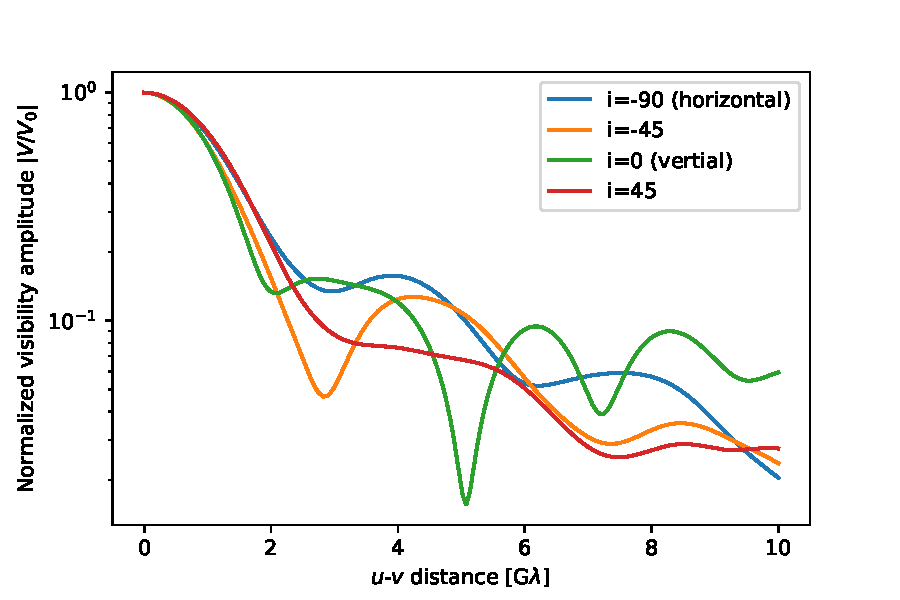
\includegraphics[width=0.5\textwidth]{figures/SANE_va.pdf}%
  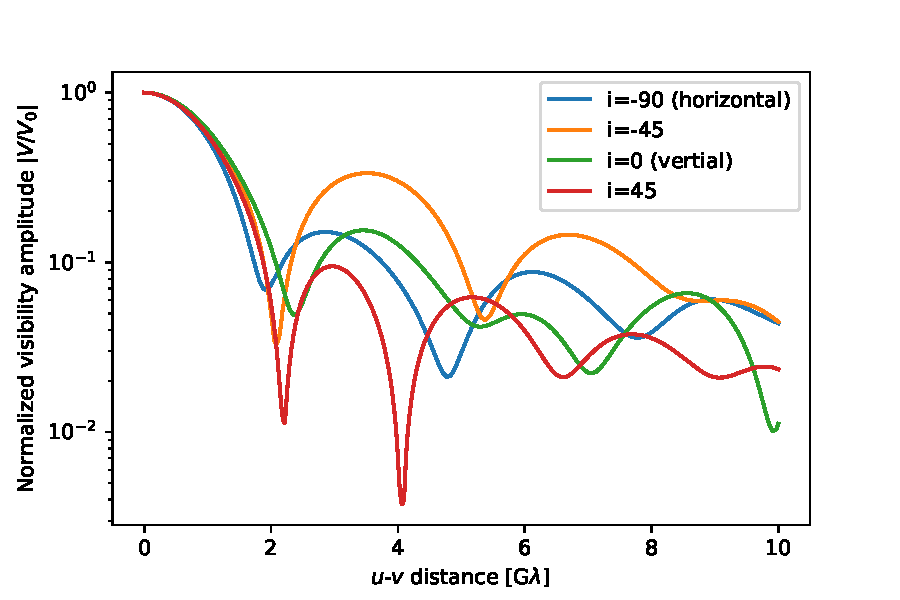
\includegraphics[width=0.5\textwidth]{figures/MAD_va.pdf}
  \caption{The left panels show two snapshots from a GRMHD simulation
    with SANE field configuration and black hole spin $a=0.5$ and the
    right panels the corresponding visibility amplitudes for a
    horizontal and a vertical cross section through the images.
    The snapshot in the top row obeys both selection criteria: the
    minima are in the 2.5-3.5 G$\lambda$ range and the amplitude in
    the $6-8$G$\lambda$ is below 6\%.
    The image in the bottom row, on the other hand, is an example that
    has no minimum in one cross section and too much power at long
    baselines, due to the asymmetry introduced by a transient bright
    structure in the flow.
    \ckc{The above plot looks odd because it's just one of the snapshot.  Do we want to show the mean?  The range?}
    \aeb{A few very minor pedantic points: 1. Can we fix the plot domain to avoid the sudden ending of lines?  They are misleading in that they seem to show an end to a function that certainly continue. 2. The fonts are wrong and the font size is too small.  3. Colors are not being used effectively to indicate conceptual closeness.  4. This plot fails the Jon Aarons test: if it were printed in grayscale or seen by a colorblind individual it would be impenetrable.}}
  \label{fig:cmp_VA}
\end{figure*}

%\begin{figure}
%  \centering
%  \includegraphics[width=0.5\textwidth]{figures/va_compare.pdf}
%  \caption{Visibility amplitude as a function of baseline length
%    observed on 2017 April 7.
%    The pink band marks the location of the first minima in the
%    visibility amplitude along different orientations.
%    The horizontal red line marks our conservative upper limit for the
%    observed visibility amplitude between $6-8$G$\lambda$.}
%  \label{fig:cmp_null}
%\end{figure}

%\begin{figure}
%  \centering
%  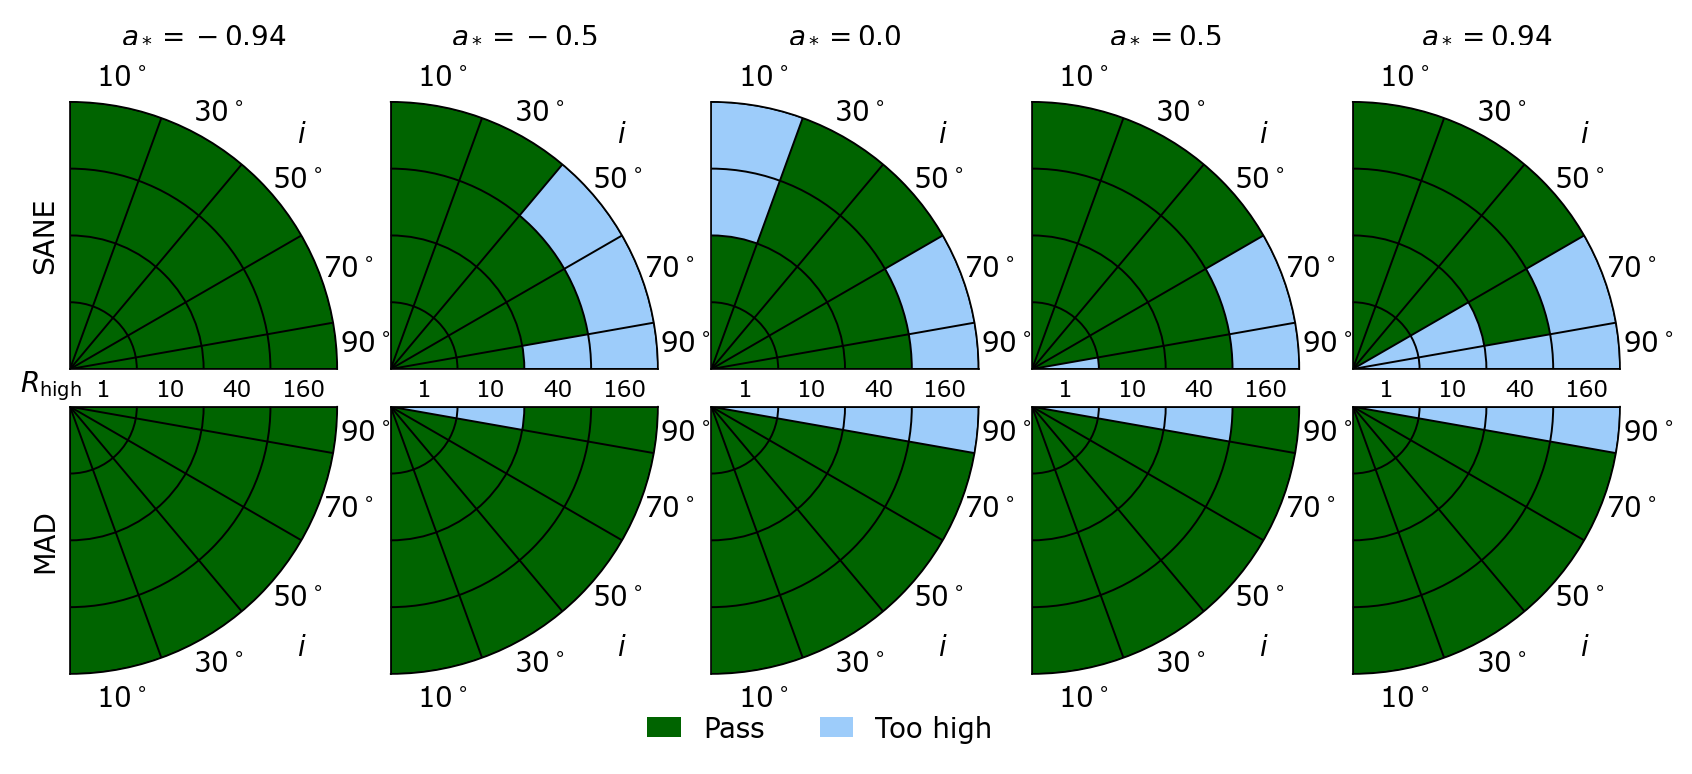
\includegraphics[width=\columnwidth]{./figures/Null_loc_Constraints.png}
%  \caption{Null Location Constraint\ckc{Texts/labels in pizza plots too %small to read.}}
%  \label{fig:cmp_ozel}
%\end{figure}

The null location constraint is a simple comparison between the model and observed variability amplitude.
It disfavors edge-on MAD models at positive spin and a few large $\Rh$ SANE models.
The null location constraint passes 77\% of models.

%..............................................................................
\subsubsubsection{Second Moment}

%\begin{figure}
%  \centering
%  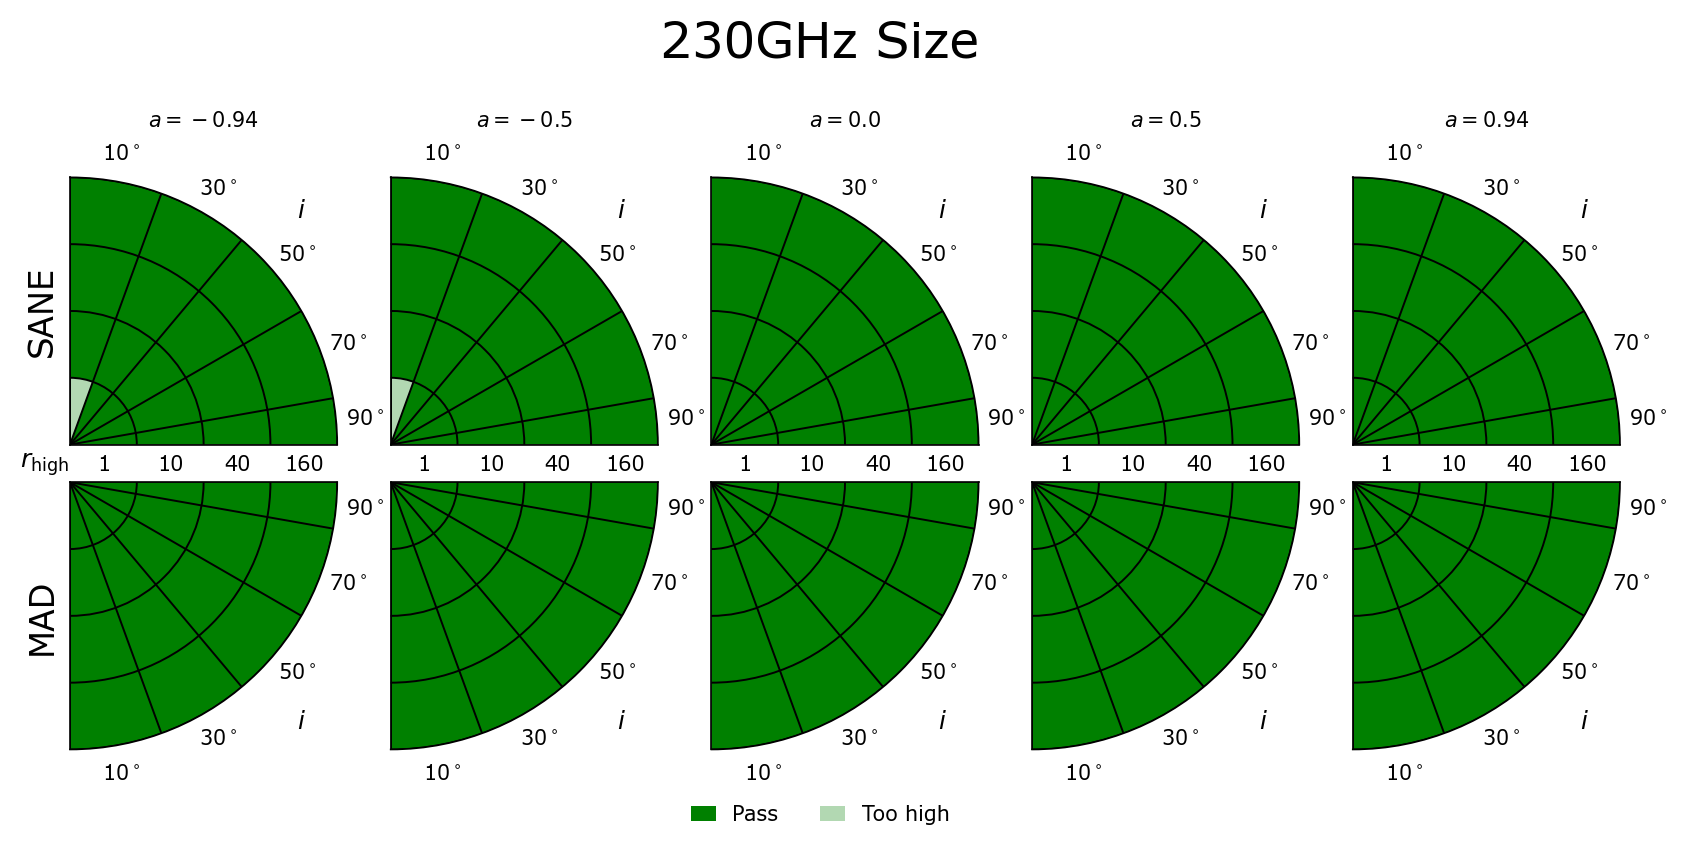
\includegraphics[width=\columnwidth]{./figures/230GHz_size_Constraints.png}
%  \caption{2nd moment plots}
%  \label{fig:cmp_2nd_moment}
%\end{figure}

The second moment constraint passes 99\% of models, that is, the models are all crudely the right size.  The models that fail are retrograde, face-on, SANE models with $\Rh = 1$. These models have extended rings of emission with angular extent that is large compared to the critical impact parameter.

%..............................................................................
\subsubsubsection{M-ring Fits}
\label{sec:mring}

The m-ring fits pass 94\%, 65\%, and 36\% of models for the ring asymmetry, diameter, and width respectively.

The asymmetry parameter is typically not very well constrained.  The models that fail are almost all high inclination models with positive spin.  The failing models have asymmetries that are large and detectable because Doppler boosting concentrates emission in an equatorial spot on the approaching side of the disk.

%\begin{figure*}
%  \centering
 % 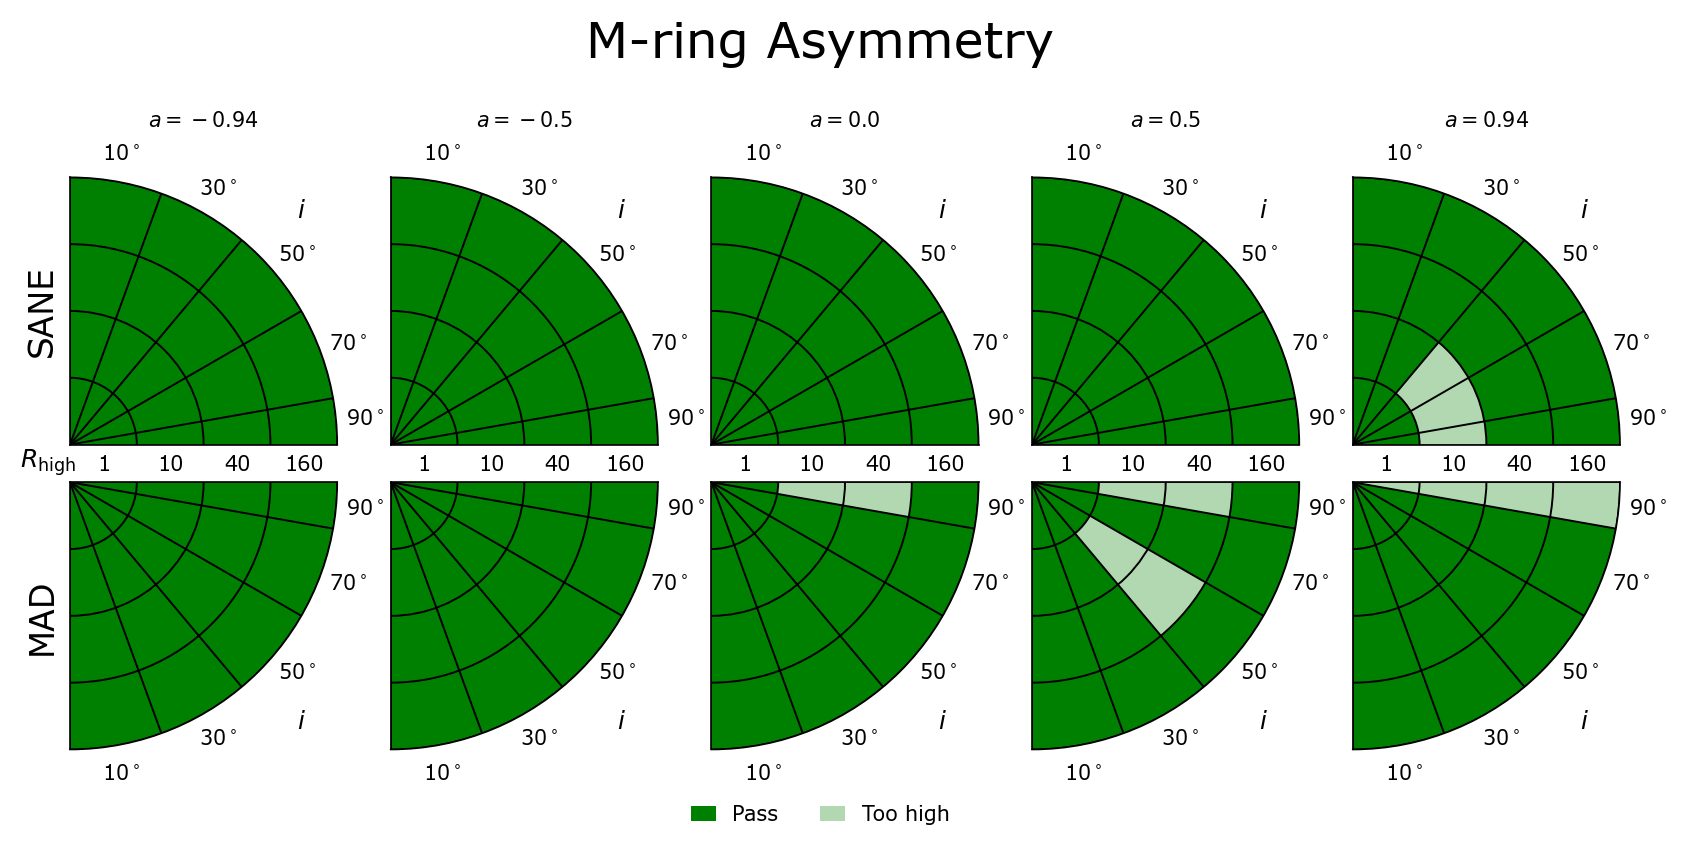
\includegraphics[width=\columnwidth]{./figures/Mring_f1_Constraints.png}
%  \caption{m-ring asymmetry}
%  \label{fig:cmp_m-ring_asymm}
%\end{figure*}

The ring diameter is better constrained than the asymmetry parameter.  It also varies systematically from model to model.  A much larger fraction of models therefore fails the ring diameter test.

Most of the models that fail are low inclination models with ring diameters that are too large (only one model fails because the ring diameter is too small).  For example, the face-on, $\Rh = 10$ SANE models fail for all spins except $\abh = 0.94$ because the ring is too large.  The same is true for all face-on MAD models with $\Rh = 1$.

\begin{figure*}
  \centering
  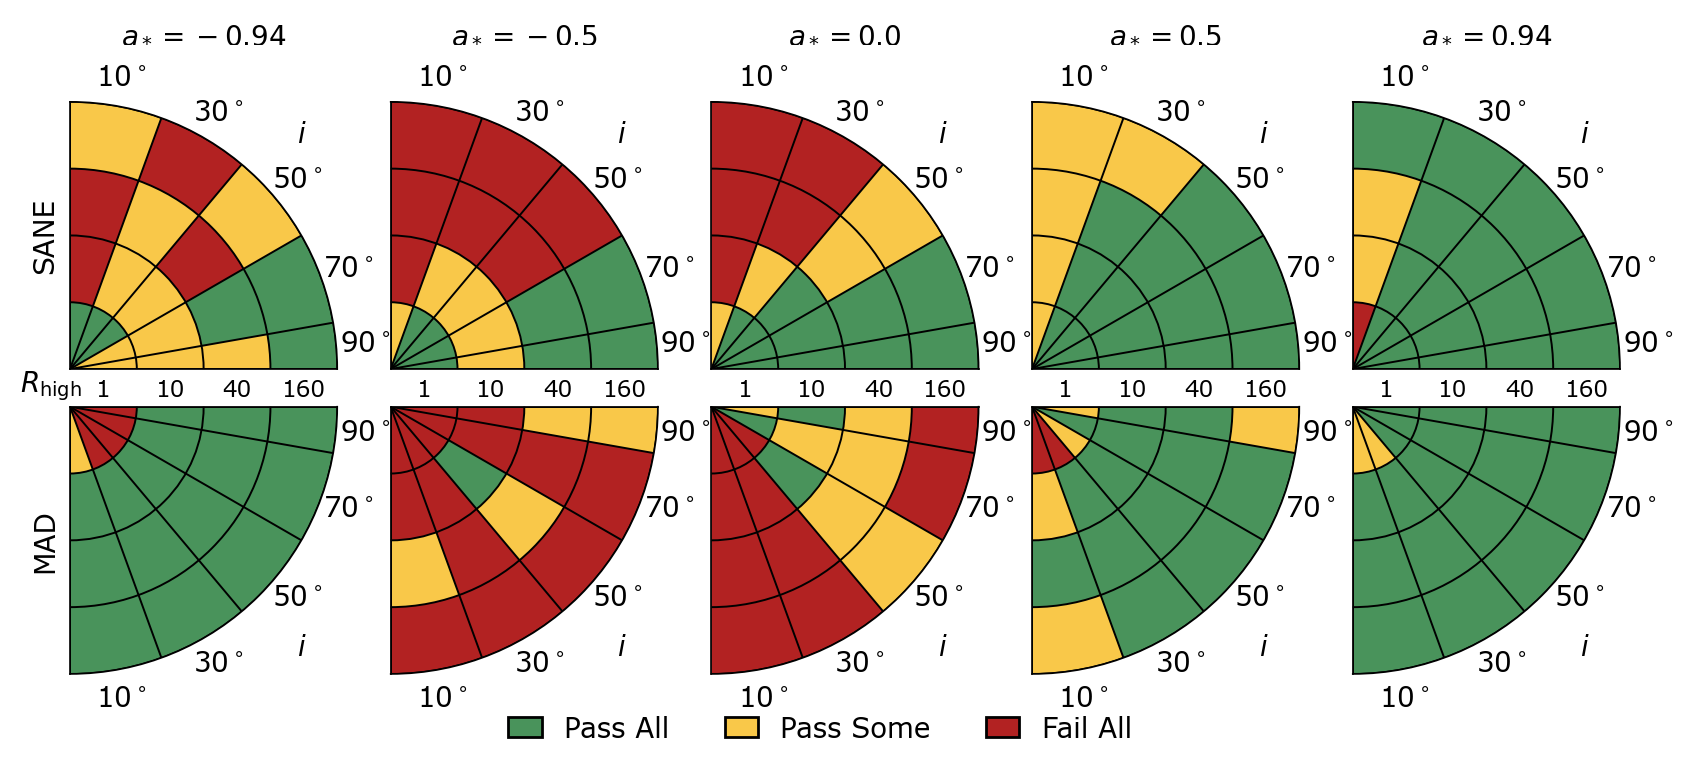
\includegraphics[width=\textwidth]{./figures/Mring_d_Constraints.png}
  \caption{M-Ring diameter.}
  \label{fig:cmp_m-ring_diam}
\end{figure*}

The m-ring width is best constrained and therefore most constraining.  Although the closure phases constrain the m-ring width as well, it is easy to see how the visibility amplitudes are affected by m-ring width: the width controls long-baseline amplitudes. Smaller width for a simple, symmetric ring corresponds to larger visibility amplitudes on long baselines.

All models that fail have m-ring widths that are too small.  This includes all but 3 MAD models at $\abh \le 0$ and all MAD models at $i = 90\degree$.

\begin{figure*}
 \centering
 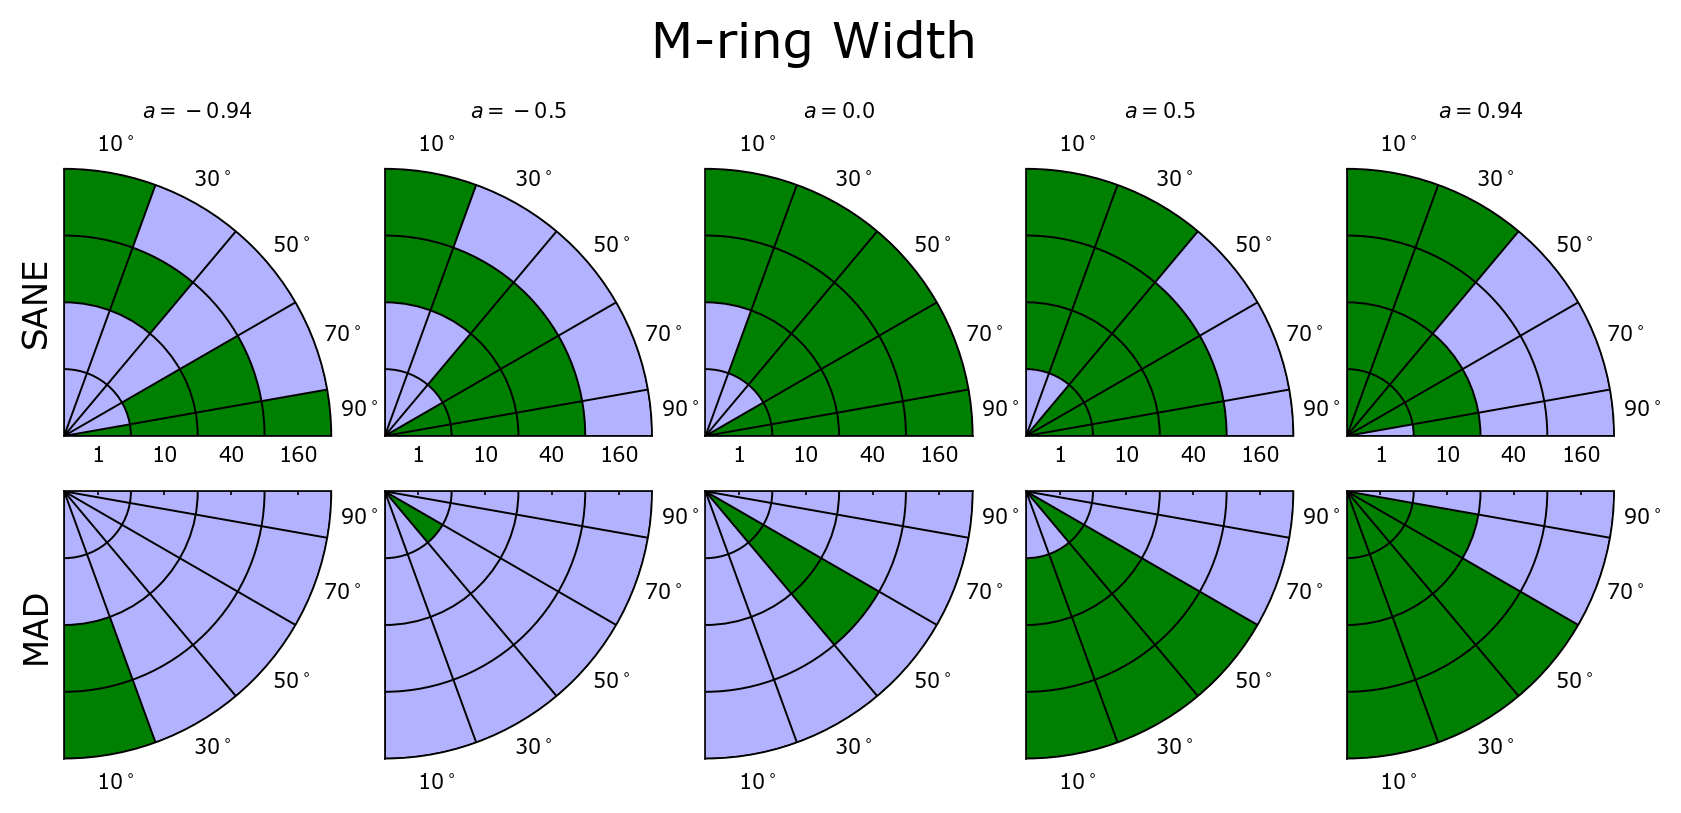
\includegraphics[width=\textwidth]{./figures/Mring_w_Constraints.png}
  \caption{m-ring widths}
% \label{fig:cmp_m-ring_width}
\end{figure*}

\subsubsubsection{EHT Constraint Summary}

Constraints based on EHT data are summarized in Figure \ref{fig:all_EHT_constraints}.  The cuts favor $\abh > 0$ models.  We are left with $31/100$ SANE models and $20/100$ MAD models.

\begin{figure*}
  \centering
    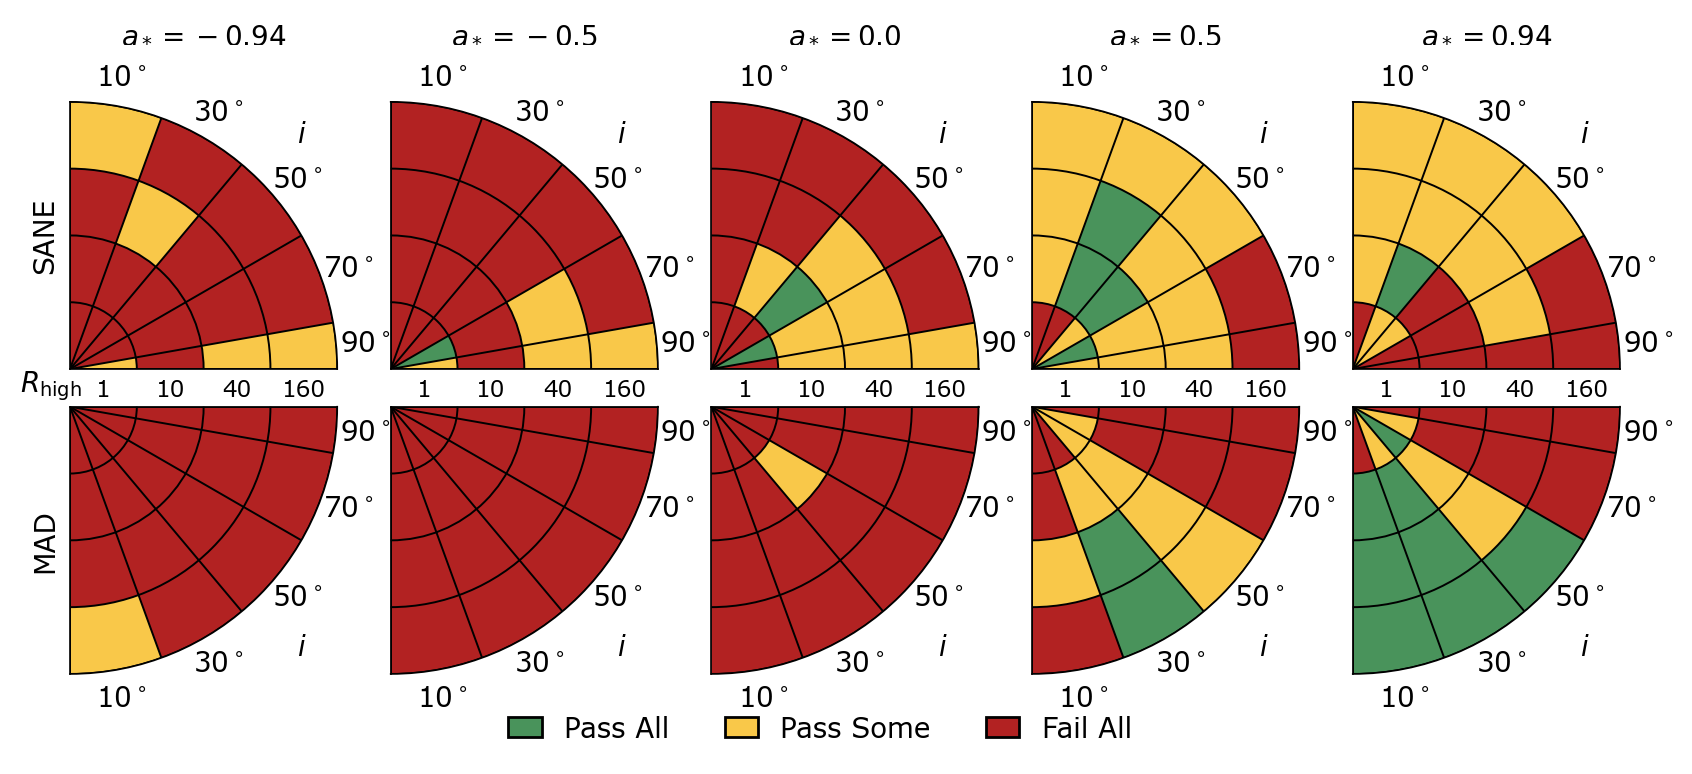
\includegraphics[width=\textwidth]{./figures/Interferometric_Constraints.png}
  \caption{Combined EHT constraints (logical {\em and}) including the second moment, null location, and m-ring fit constraints.}
  \label{fig:all_EHT_constraints}
\end{figure*}

\subsubsection{Non-EHT Constraints}

Now consider constraints from 86GHz, NIR, and X-ray observations.  Most or all of the emission in these bands is believed to originate in the compact source from plasma that is close to or overlaps the plasma the 230GHz-emitting plasma observed by EHT.

%..............................................................................
\subsubsubsection{NIR Median Flux}

NIR photons are produced by synchrotron process from photons at the high energy end of the distribution function.  For a one-zone model with $B = 30$G, the  critical frequency $\nu_{crit} \simeq \gamma^2 e B/(m_e c) \simeq 80$GHz and emission at $2.2\mu$m is therefore produced by electrons with $\gamma \simeq 10^3$, compared to a mean Lorentz factor of $30$ for plasma with $\Theta_e = 10$.  NIR flux density will therefore be sensitive to $\Theta_e$ and therefore to $\Rh$.

Interestingly, we find that some models are synchrotron-weak and Compton-strong in the NIR.  \note{Discussion of which models fall in this category}

Models that pass the NIR flux limit are shown in Figure \ref{fig:cmp_2um_flux}.

All but $6\%$ of the SANE models pass; the exceptions are high spin, high inclination models where Doppler boosting increases the NIR flux from the bright spot on the approaching side of the disk.  Considering MAD models alone, $68\%$ fail the NIR test, including all but 1 model at $\Rh = 1$ and $10$.

%\begin{figure}
%  \centering
%  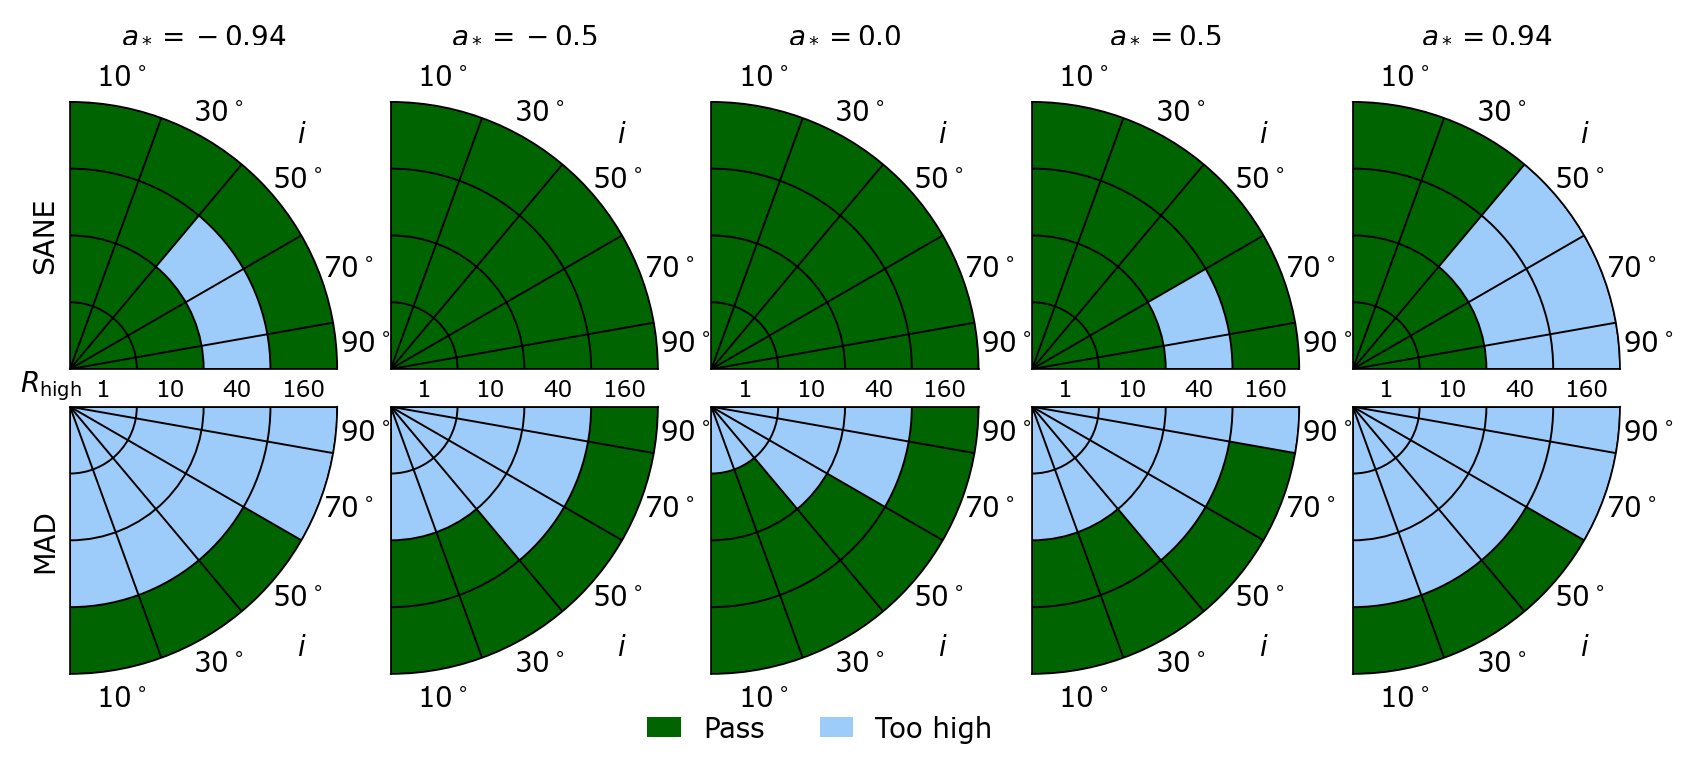
\includegraphics[width=\columnwidth]{./figures/2um_flux_Constraints.png}
%  \caption{NIR flux limit}
%  \label{fig:cmp_2um_flux}
%\end{figure}

%..............................................................................
\subsubsubsection{X-ray Luminosity}

Most thermal models produce X-ray emission through Compton upscattering of thermal synchroton photons.  Typically the X-ray band lies in the first Compton bump, although that is sensitive to the temperature of the electrons doing the upscattering.  In the first Compton bump $\nu L_\nu$ is proportional to the y-parameter $y \sim 16 \Theta_e^2 \tau_e$ where $\tau_e$ is a characteristic electron-scattering optical depth and $\Theta_e$ is a typical electron temperature.

In many large $\Rh$ SANE models, however, X-ray emission is dominated by bremsstrahlung.  Since the bremsstrahlung emissivity $\propto n^2$, bremsstrahlung comes from the midplane where the density is largest, at larger radius than the synchrotron and Compton-upscattered X-ray emission.  It dominates in high accretion rate models (this turns out to mean large $\Rh$ models; see \S 5) where $\Theta_e < 1$, and is significant only when the midplane is cool and $r: \Theta_e = 1 < YY$, i.e. at large $\Rh$.  The resurgence of bremsstrahlung in cool disks occurs because at $\Theta_e < 1$, $j_\nu \propto n^2 \Theta_e^{-1/2}$.  When the disk is cool and dense the latter is large.

The X-ray cut results are shown in Figure \ref{fig:cmp_xray_flux}.

Many large $\Rh$ SANE models fail the X-ray test: all but 3/25 at $\Rh = 160$ and all but 6/25 at $\Rh = 40$.  These models fail due to excess bremsstrahlung.

Many MAD models that fail have large absolute spin and low $\Rh$.  These models are Compton-dominated.  The midplane temperature is highest at low $\Rh$.  Since the midplane contributes most of the electron scattering optical depth, low $\Rh$ models have the largest $y$ parameter and are most at risk of overproducing X-rays.

%\begin{figure}
%  \centering
%  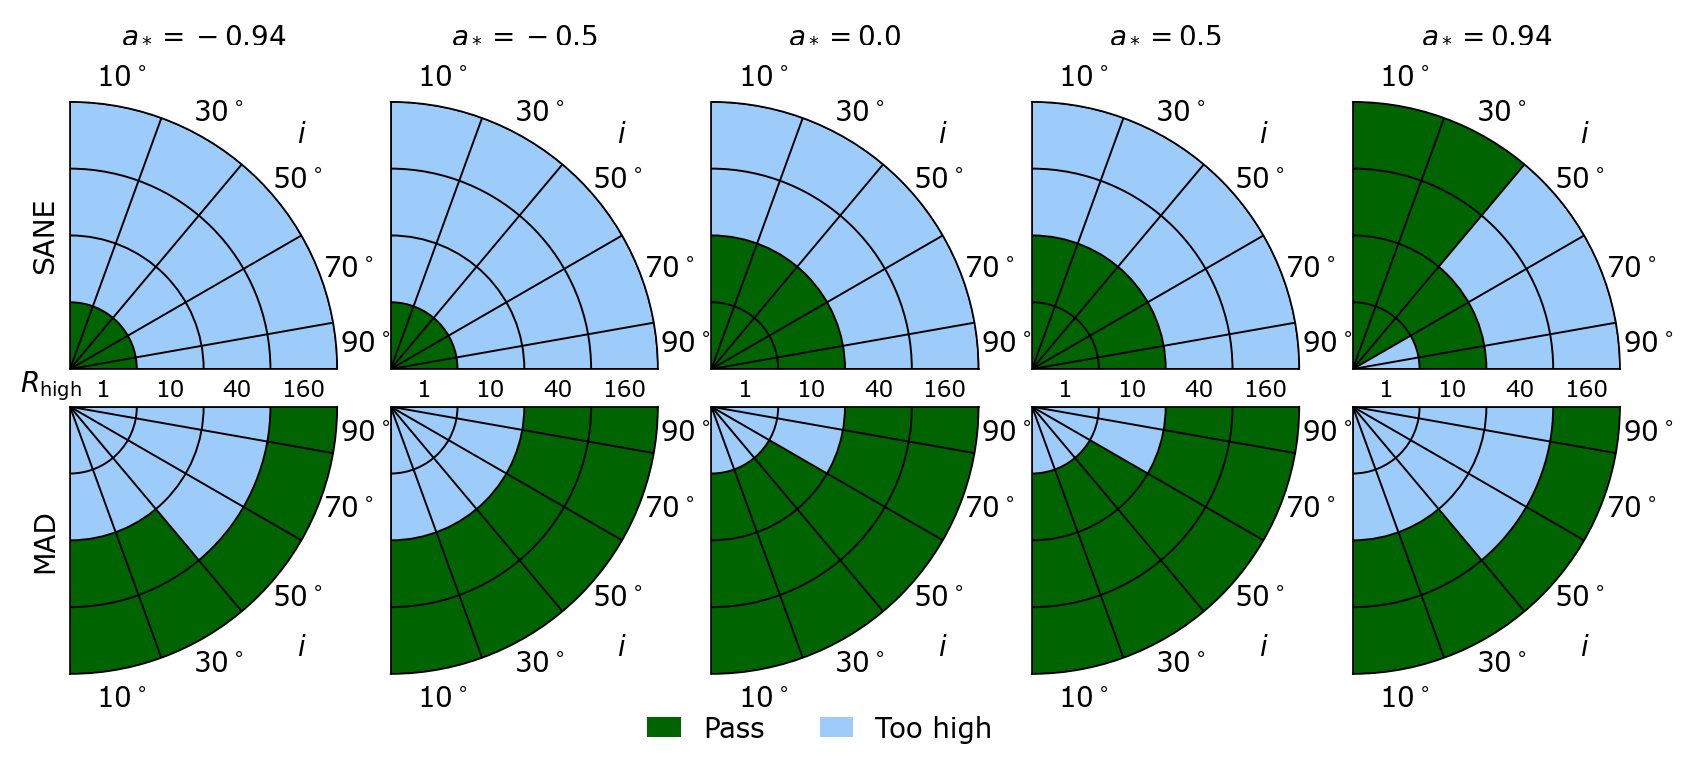
\includegraphics[width=\columnwidth]{./figures/Xray_flux_Constraints.png}
%  \caption{X-ray flux limits}
%  \label{fig:cmp_xray_flux}
%\end{figure}

%..............................................................................
\subsubsubsection{86 GHz Median Flux}

In a naive picture \sgra's millimeter flux is produced at a photosphere that decreases in size as frequency increases.  Because of the marginal optical depth at $1.3$mm ($\sim 0.3$ in the one-zone model) and the complicated source structure (the optical depth varies across the image; the $\tau = 2/3$ surface is non-spherical, folded, not even simply connected) this picture does not hold exactly.  Nevertheless 86GHz photons are on average produced at larger radius than 230GHz photons, and the 86GHz source size is therefore larger than the 230GHz source size; see Ricarte et al. 2022 for a discussion.

The 86GHz/230GHz color therefore probes the radial structure of the source plasma.  Figure~\ref{fig:cmp_86ghz_flux} shows the result of requiring that the 86GHz flux match the observed flux 3 days before the beginning of the EHT 2017 campaign.

Many $\Rh = 1$ models, both MAD and SANE, fail the $86$GHz flux density test: 23/25 SANE and 9/25 MAD.  These models overproduce $86$GHz emission.
There is also a substantial set of SANE models, 19/100 in all, that underproduce $86$GHz emission.  These models have larger $\Rh$.

%\begin{figure}
%  \centering
%  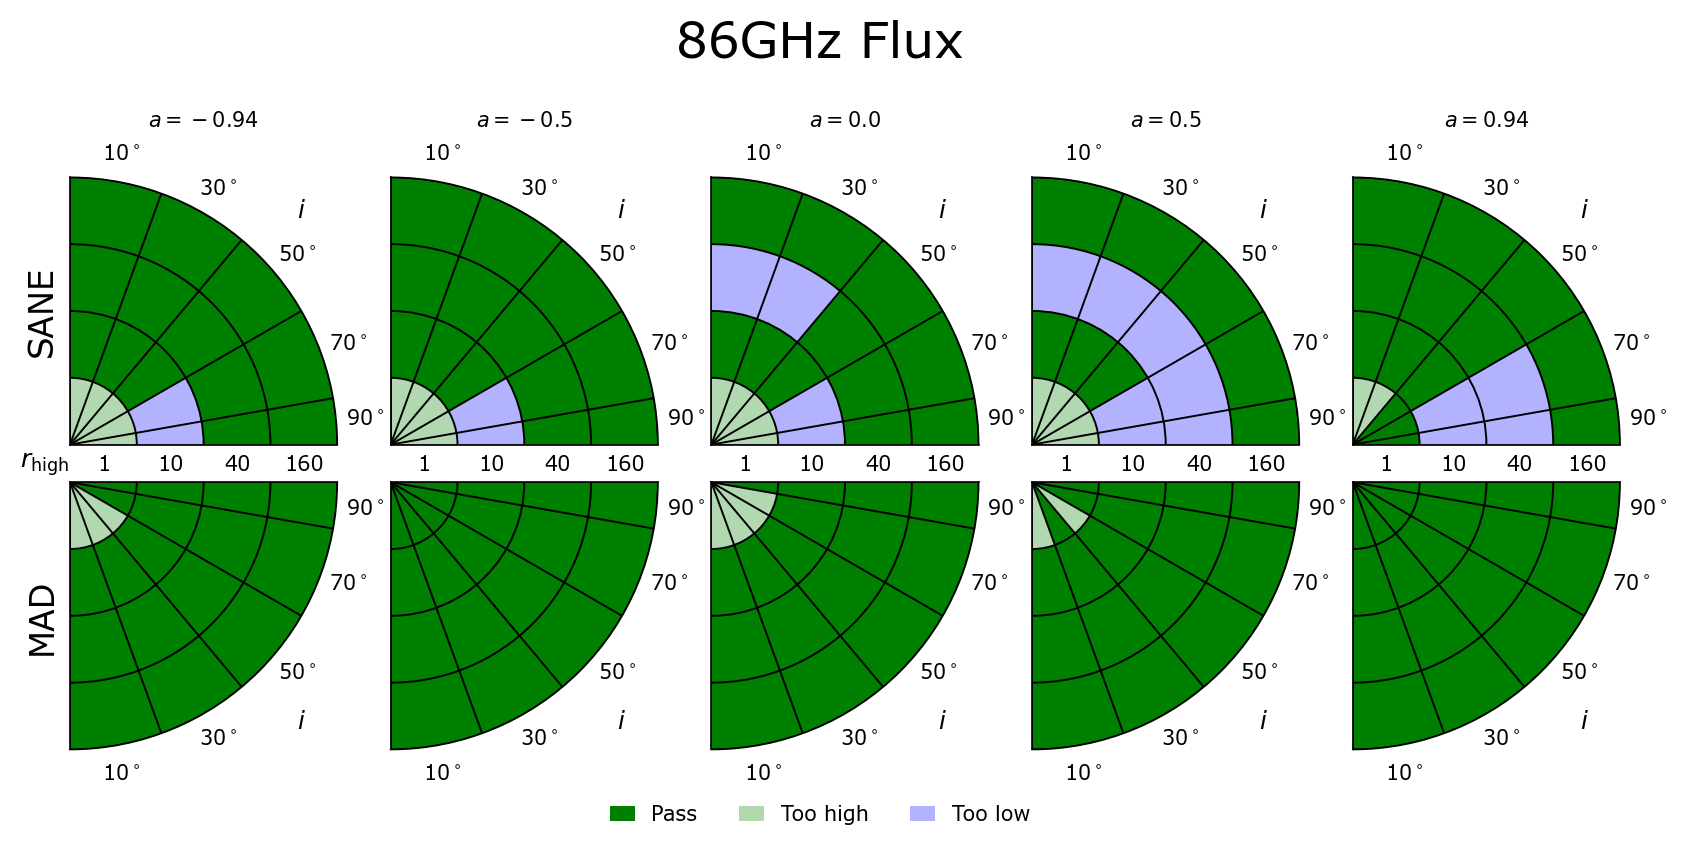
\includegraphics[width=\columnwidth]{./figures/86GHz_flux_Constraints.png}
%  \caption{86GHz flux limits}
%  \label{fig:cmp_86ghz_flux}
%\end{figure}

%..............................................................................
\subsubsubsection{86 GHz Major Axis}

As for the $86$GHz flux, the $86$GHz size is sensitive to optical depth as a function of radius in the source plasma. Models that pass and fail are shown in Figure \ref{fig:cmp_86ghz_size}.

Many face-on models fail because they are too small (purple in the figure), while a few other high inclination models fail because they are too large.  Only $52\%$ of models pass, making this one of the tightest constraints.

The physical picture for 86GHz source size is complicated, as is the extraction of the constraint itself from observations.  Notice that (1) two different values for the 86GHz intrinsic source size have been reported in the literature; (2) scattering is $7$ times stronger at $86$GHz than at $230$GHz; (3) scattering must be subtracted accurately to obtain the intrinsic source size; (4) the error bars for the 86GHz source size are narrow and this determines the strength of the constraint.

%\begin{figure}
%  \centering
%  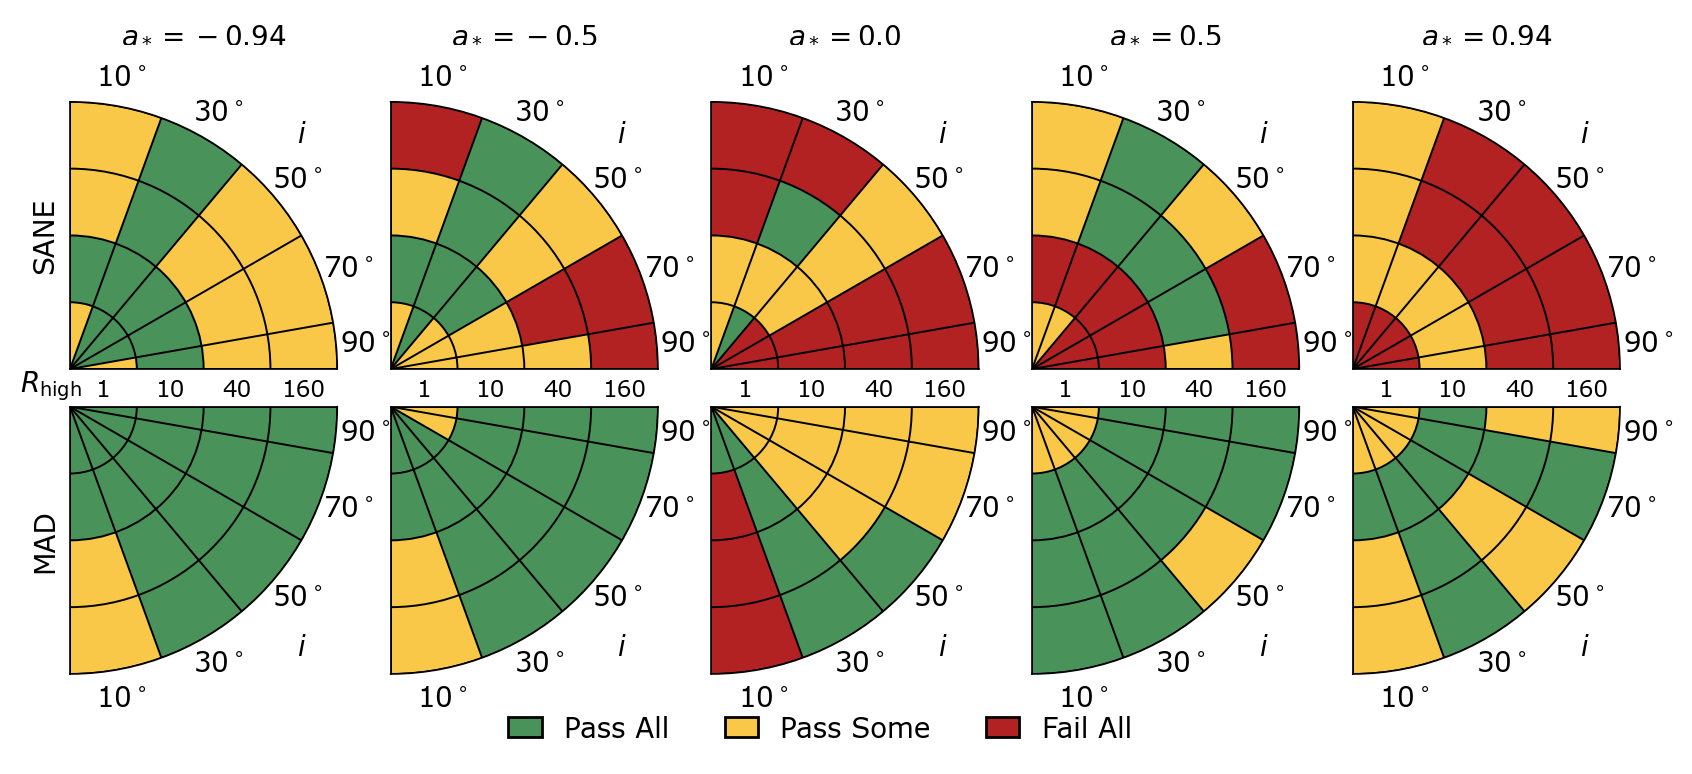
\includegraphics[width=\columnwidth]{./figures/86GHz_size_Constraints.png}
%  \caption{86GHz size}
%  \label{fig:cmp_86ghz_size}
%\end{figure}

%..............................................................................
\subsubsubsection{Summary of Non-EHT constraints}

Applying only non-EHT constraints, we are left with the 9/100 SANE models and 25/100 MAD models shown in Figure~\ref{fig:non_eht_cuts}.

The surviving models include a set of SANE models at intermediate $\Rh$ and modest inclination, as well as MAD models at large $\Rh \ge 40$. No $\Rh = 1$ models survive the non-EHT cuts.

\begin{figure*}
  \centering
  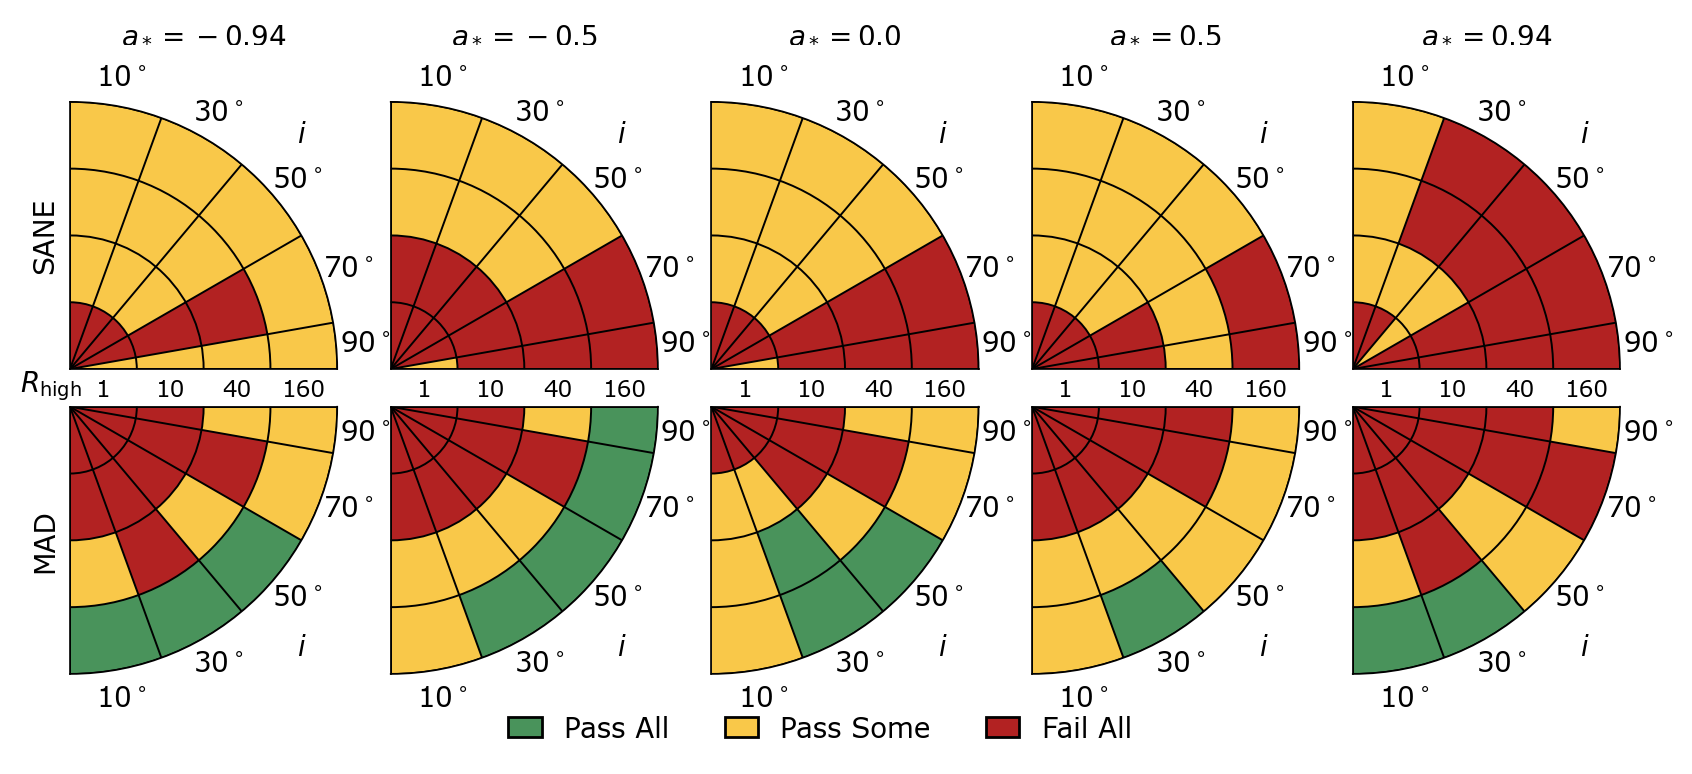
\includegraphics[width=\textwidth]{./figures/Non_Interferometric_Constraints.png}
  \caption{Combined non-EHT constraints}
  \label{fig:non_eht_cuts}
\end{figure*}

%------------------------------------------------------------------------------
\subsubsection{Variability}

Variability is central to interpretation of \sgra: the small black hole size means that observations considered here are taken over intervals when the source is expected to vary significantly.  This distinguishes \sgra from \m87, where the source is expected to vary only over timescales that are long compared to a single track.\footnote{This does not mean that \m87 is less variable than \sgra.  In 2017 EHT observed \m87 over only $\sim 15\tg$\monika{1 week is 168h and \tg for m87 is 8.5h, this gies 19 \tg not 15...}, so it is not possible to characterize \m87 variability using EHT data alone.  To obtain variability information for \m87 similar to what we present here for \sgra would require multi-year observations.}

Variability is a strong constraint on the models.  Although models differ in their degree of variability, both in an integrated sense and on 4 $G\lambda$ baselines, only a small fraction of models are as quiet as the data.  For the light curve variability, this remains true whether we use data from 2017 April 7, all days from the 2017 observing campaign, or from historical monitoring of \sgra.   In general, we find that SANE models are quieter than MAD models, and (less strongly) face-on models are quieter than edge-on models.

If we were to apply the variability constraints directly to the models, there would be 30/200 successful models left using 1\% cuts (47/200 for the ALMA constraint and 95/200 for the visibility amplitude constraint).  One interpretation of this result is that the surviving models are the correct description of the source (although we would expect some misclassification of models as consistent or inconsistent when using 1\% cuts on such a large model set).  Another interpretation is that there is a missing physical ingredient in the models, see Section \ref{sec:discussions} for a discussion.

%..............................................................................
\subsubsubsection{ALMA Light Curve}

The distributions of 3 hour modulation index (rms \%) across all SANE models, across all MAD models, and across the historical dataset are shown in Figure \ref{fig:cmp_ALMA_var}, along with individual distributions for the models with the lowest and highest MI for SANEs and MADs. Although some individual models  pass (particularly SANE models), the distributions for the SANEs and the MADs are noticeably offset from the data, with the MADs in particular being more variable. As can be seen, even the quietest MAD model lies above the historical distribution.

If we compare each individual model to the three segments from the 7 April 2017 ALMA observation using a 2-sample KS test, eliminating models with $p < 1\%$, we are left with 56 SANE models and 9 MAD models.

If we instead compare the models to the full historical distribution (40 measurements of $\mi{3}$ in all, including ALMA), we find that 47 SANE models and no MAD models pass. This is more stringent than the comparison with just 7 April, since the historical distribution has more samples and thus disparate models can be eliminated with higher confidence.

\begin{figure}
  \centering
  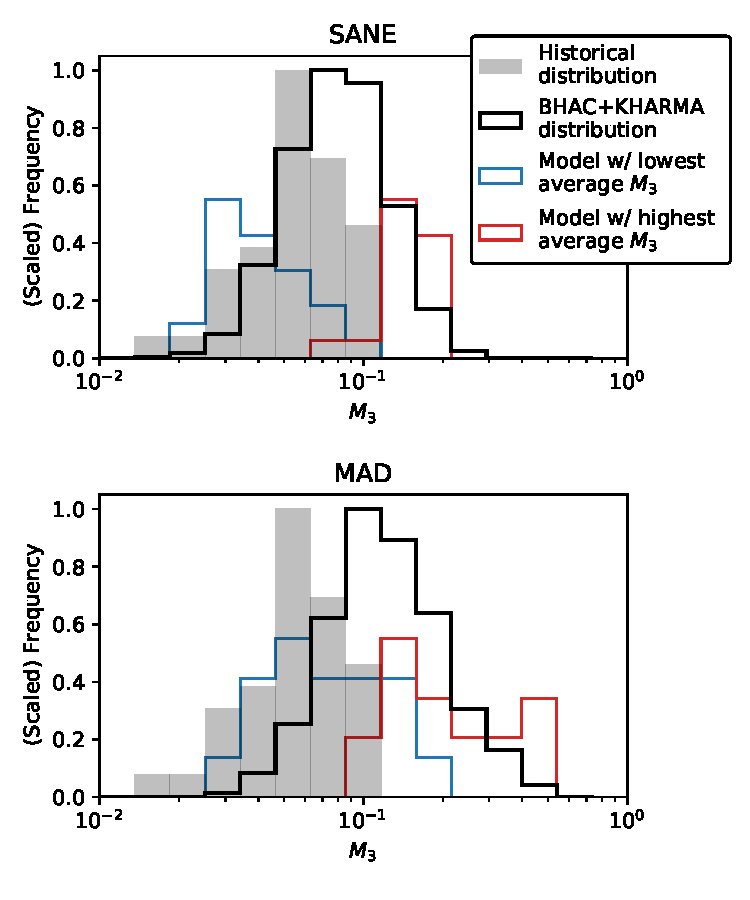
\includegraphics[width=\columnwidth]{./figures/mi_hist.pdf}
  \caption{Distributions of $\mi{3}$ for \kharma models (black), compared to distributions from historical observations (gray). The distributions for models with the lowest (blue) and highest (red) average $\mi{3}$ for SANEs and MADs are also shown. The heights of these distributions have been scaled down for visual clarity.
  }
  \label{fig:cmp_ALMA_var}
\end{figure}

%..............................................................................
\subsubsubsection{4 $G\lambda$ Visibility Amplitude Variability}

The power-law indexes of the variance $\sigma_\text{var}^2 (|u|)$ at $4~{\rm G}\lambda$ of the GRMHD models is generally in good agreement with the measured value of $b$ from the 2017 EHT campaign (excluding April 11). The amplitude $\afour^2$, however, varies depending on the model and the code.

Figure~\ref{fig:cmp_VLBI_var} shows the distribution of $(\afour^2, b)$ from the EHT observation, along with the distribution across all \kharma models. The GRMHD models are shown as an aggregate whole, but each model consists of only three measurements of $\afour^2$, one on each window. This makes a direct comparison with the measured value difficult, as the distribution for a given model is poorly constrained.

\citet{Georgiev_2022} gives an estimate for the width of the distribution as $\log_{10}(\afour^2) \pm 0.1$. We can get a rough estimate for how the GRMHD models fare compared to the measurement by taking the mean across windows and the estimate for the width, and comparing this with the measurement distribution under the assumption that both are distributed normally. Under this, 95/200 models (50 SANE and 45 MAD) agree with the data within 1\%, although we caution against interpreting this number as the number of passing or failing models, since the uncertainties in the model distribution are so large.

Overall, the GRMHD models tend to be slightly more variable than the measured value, with face-on models performing better than edge-on models. For SANE models, $\Rh = 10$ tend to be more variable than others. For MAD models, there is a slight preferance for lower $\Rh$.

We have also considered a set of thermal, $\Rh$, MAD models run with the \koral code out to $\sim 100,000\tg$.  These models permit us to assess the importance of integration time for application of the constraints.  They permit us to obtain more accurate distributions for the constraint quantities, and to assess whether the constraints evolve from the beginning to end of the integrations. We do not see evidence for evolution in the \koral model set (a full pass/fail table is given in Appendix~\ref{app:tables}, Table~\ref{tab:koralPF} and more detailed discussion in Appendix~\ref{app:variability}). The \koral pass/fail results are similar to those for comparable models in the \kharma thermal model set. Moreover the constraints measured at the beginning of the evolution are similar to those measured at the end.

% The distribution of model $4G\lambda$ lightcurve-normalized PSDs are shown in Figure \ref{fig:cmp_VLBI_var}.  The best fit PSD from the 2017 EHT campaign (excluding April 11) is shown as a solid vertical line, with the other vertical lines showing percentiles in the posterior.  Evidently the observations are quieter than both SANEs and MADs as a group.

% The PSD estimates for the models are broken up into $5000\tg$ windows for each model. To compare the models to the observation, we take the mean value across all windows and assume the width of the distribution is of $\log_{10} a_{4G\lambda} \pm 0.1$. A model is considered passing if this estimated distribution overlaps with the median observed value. \note{refer GRMHD variability paper appendix} \dl{passing criterion subject to change}

% With this approach only 6\% of the models pass, and all SANE. While the quietest models tend to be SANEs, the general distribution across all MADs is not as offset from the SANEs as in the MI distributions.

% \begin{figure}
%   \centering
%   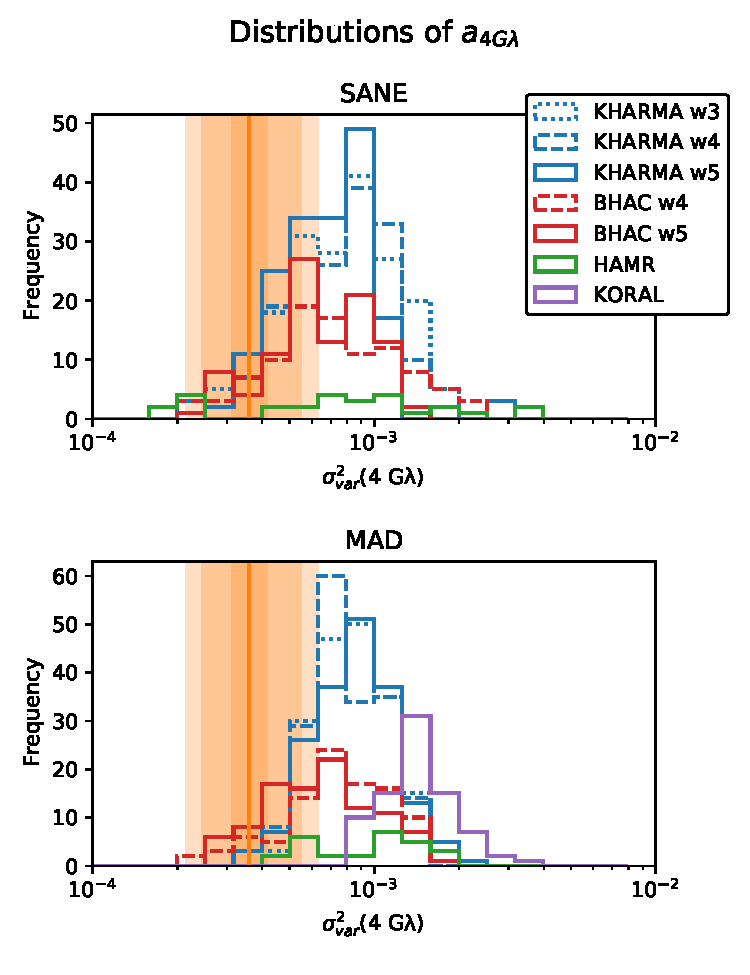
\includegraphics[width=\columnwidth]{./figures/va_hist.pdf}
%   \caption{Distributions of $PSD(4\,\mathrm{G}\lambda)$ for thermal models, compared to the observed distribution from the 2017 EHT campaign.
%   \dl{HAMR distribution will be updated later.}
%   \aeb{The quantity on the horizontal axis has been called $a_4$ in \citetalias{PaperIV}.  I have a similar concern regarding the abrupt end of the curves in this plot as well.  What do they mean?  How should these be interpreted?  There are the standard presentation issues (see \autoref{fig:cmp_VA}).}
%   \ckc{Nice new plot!  Are you using matplotlib fill\_between?  I suggest setting edgecolor to None and only set facecolor.  (Or setting linewidth=0 should also remove the lines in the orange shade.)}}
%   \label{fig:cmp_VLBI_var}
% \end{figure}

\begin{figure}
  \centering
  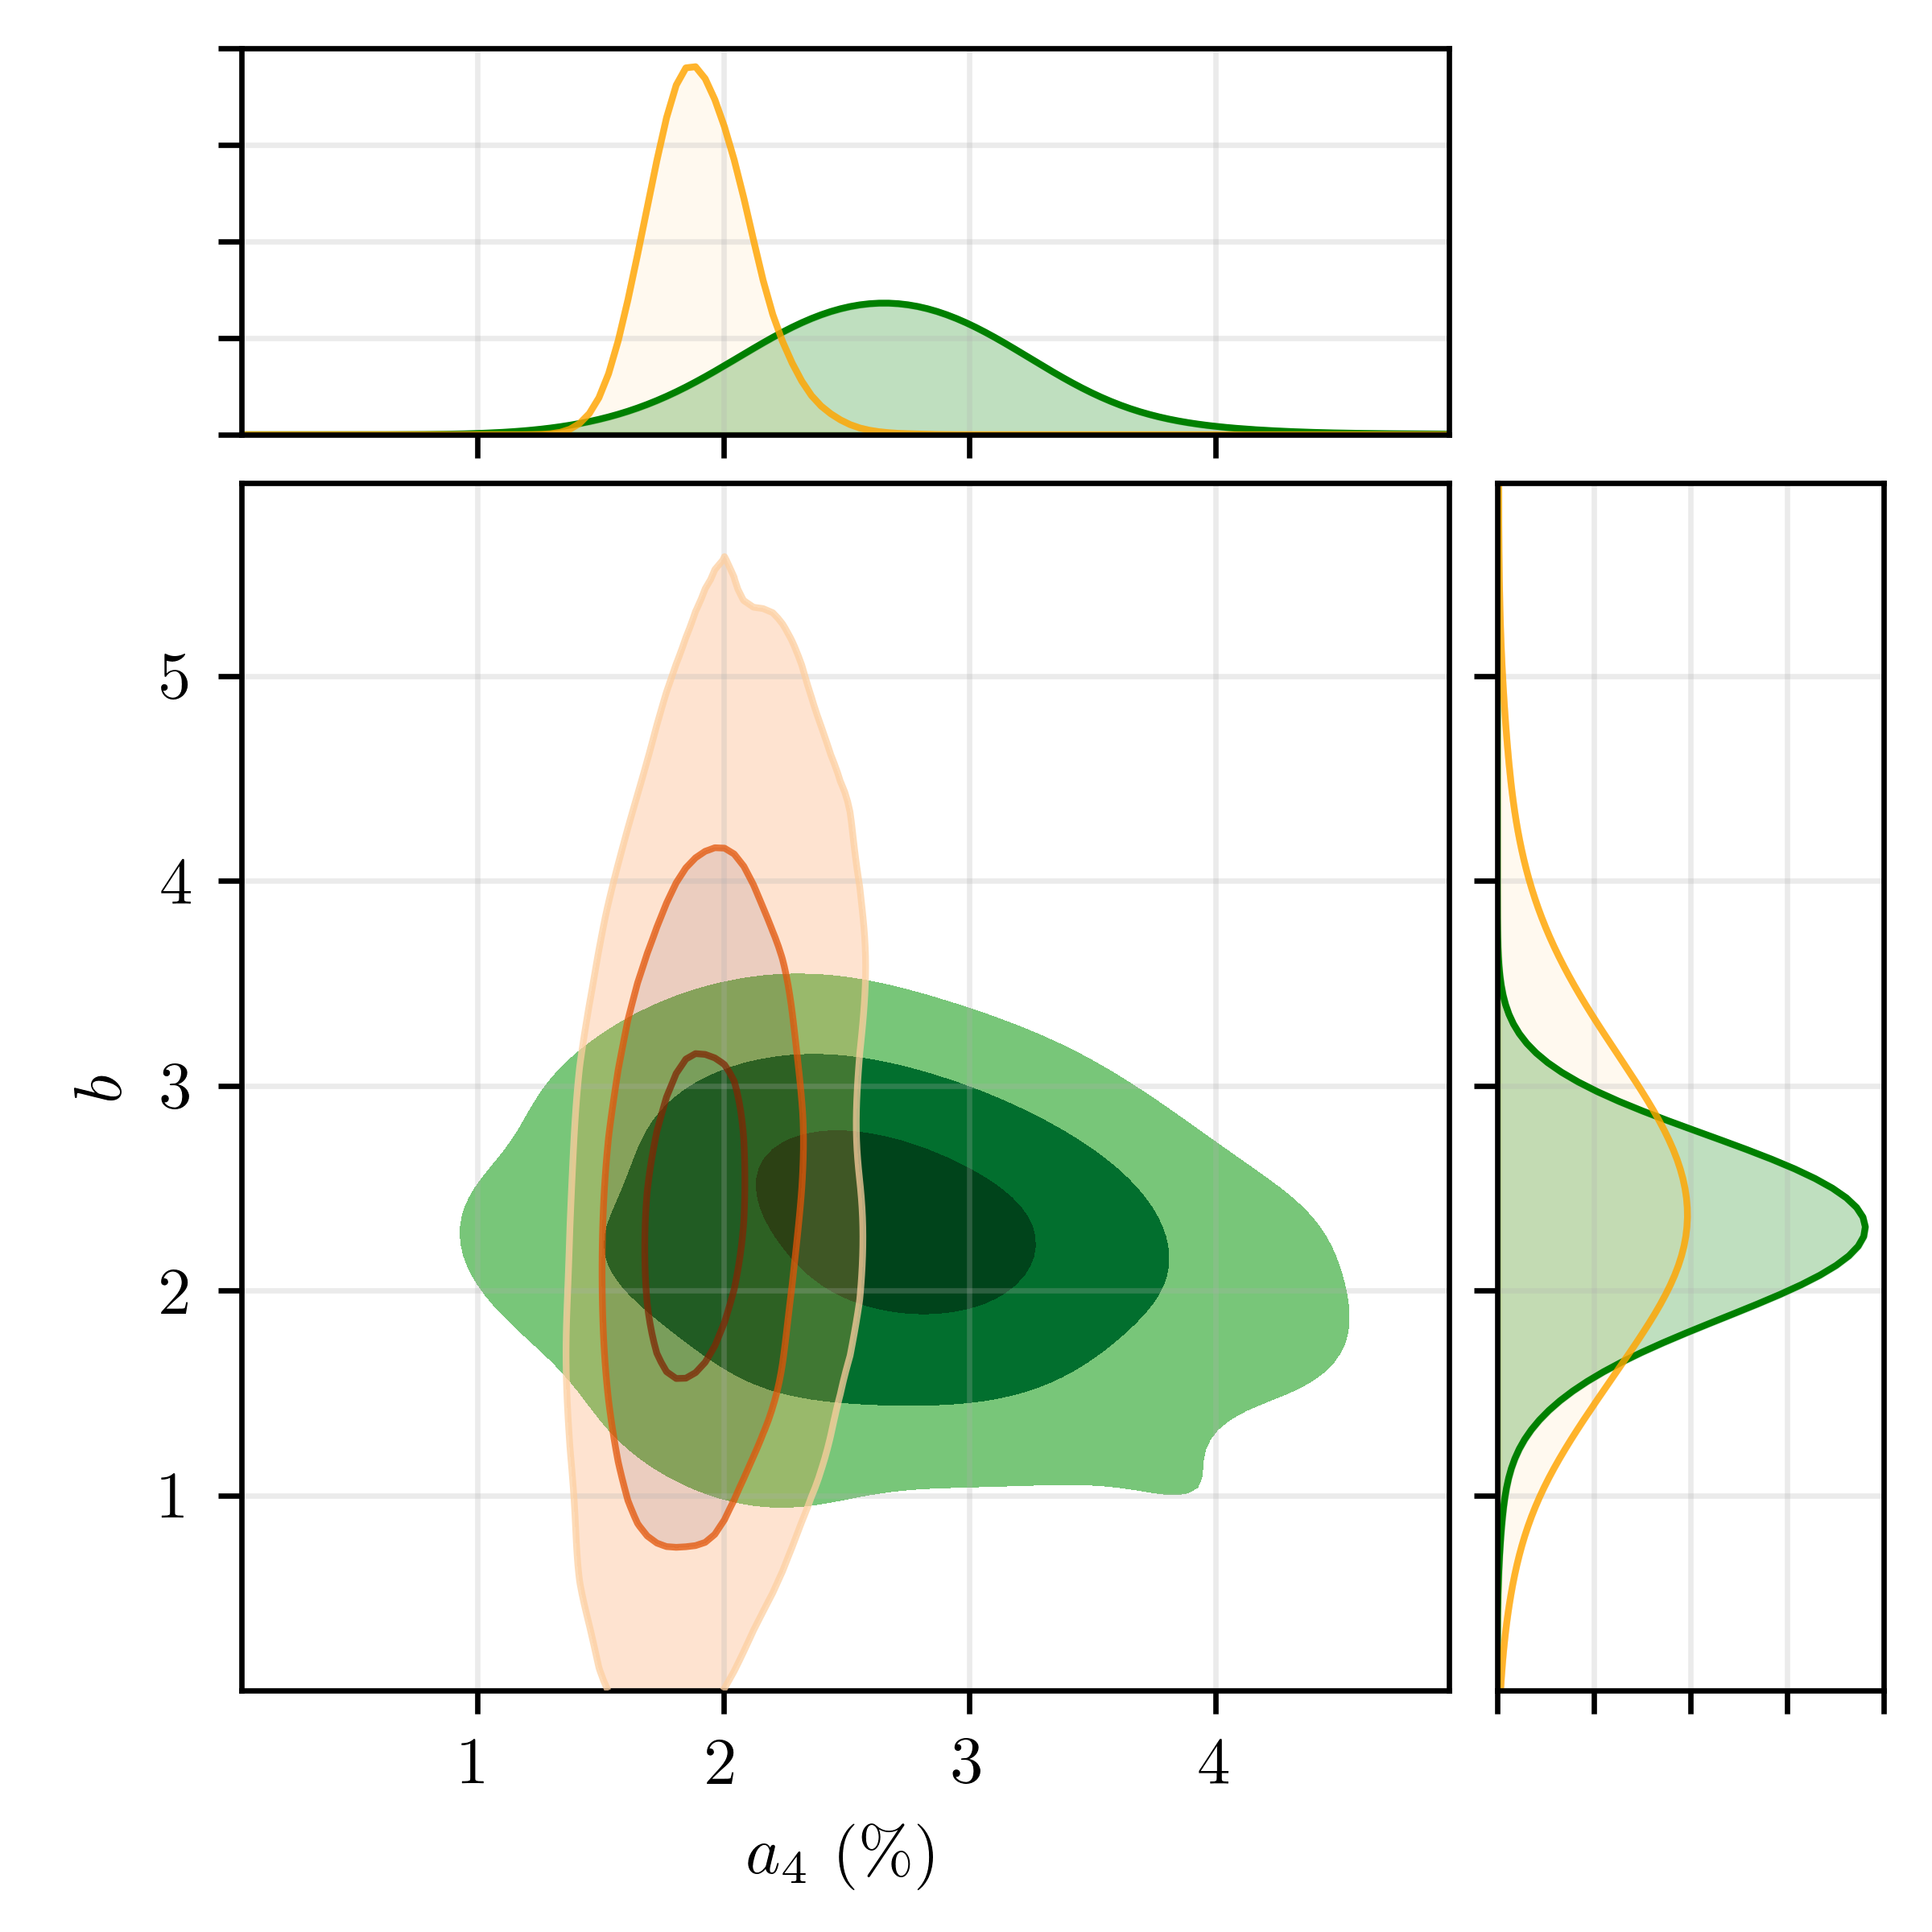
\includegraphics[width=\columnwidth]{./figures/grmhd_fit.png}
  \caption{\dl{placeholder figure}}
  \label{fig:cmp_VLBI_var}
\end{figure}

% At a 1\% cut, the models that pass the PSD constraint also all pass the MI constraint. It should be noted that this is partially because these constraints are weakly correlated \dl{also partially because we're imposing constraints differently between VLBI and light curve, and the light curve constraint is more lenient} None of the 12 models with acceptable variability pass the other tests.

%------------------------------------------------------------------------------
\subsubsection{Summary of Constraints on Thermal Models}

If we set aside variability but use all the remaining constraints we are left with the models shown in Figure \ref{fig:all_cuts}.  Only 1/100 SANE models and 8/100 MAD models survive. The passing models cluster at low inclination ($i \le 50$deg) MAD models with $\Rh > 10$.  A full set of pass/fail values is provided in Appendix \ref{app:tables}.

It is remarkable that so many of the models look like the EHT data, which lends some  confidence to the models, and that EHT data alone are capable of distinguishing between models in the model set with only $N = 6$ antennas.  Future experiments with more antennas will contain much more information and provide even tighter constraints.

All $\Rh = 1$ models have been eliminated, most by multiple constraints, and we conclude that models with equal ion and electron temperatures are unacceptable.

All models with $i > 50$deg are eliminated, most by multiple constraints, and we conclude that high inclination models are disfavored.  In the SED edge-on models have a clear signature derived from Doppler boosting, with increased NIR and X-ray flux density.  In EHT constraints many edge-on models have a clear signature derived from low m-ring widths, strong asymmetry (although only for a few models), and failed null location constraint.

For thermal model sets both EHT and non-EHT constraints individually eliminate many models, but together they eliminate all but 5\%.  The success of the models for EHT constraints (apart from variability) supports the use of the models for applying non-EHT constraints and highlights the importance of contemporaneous multiwavelength monitoring of \sgra.

\begin{figure*}
  \centering
  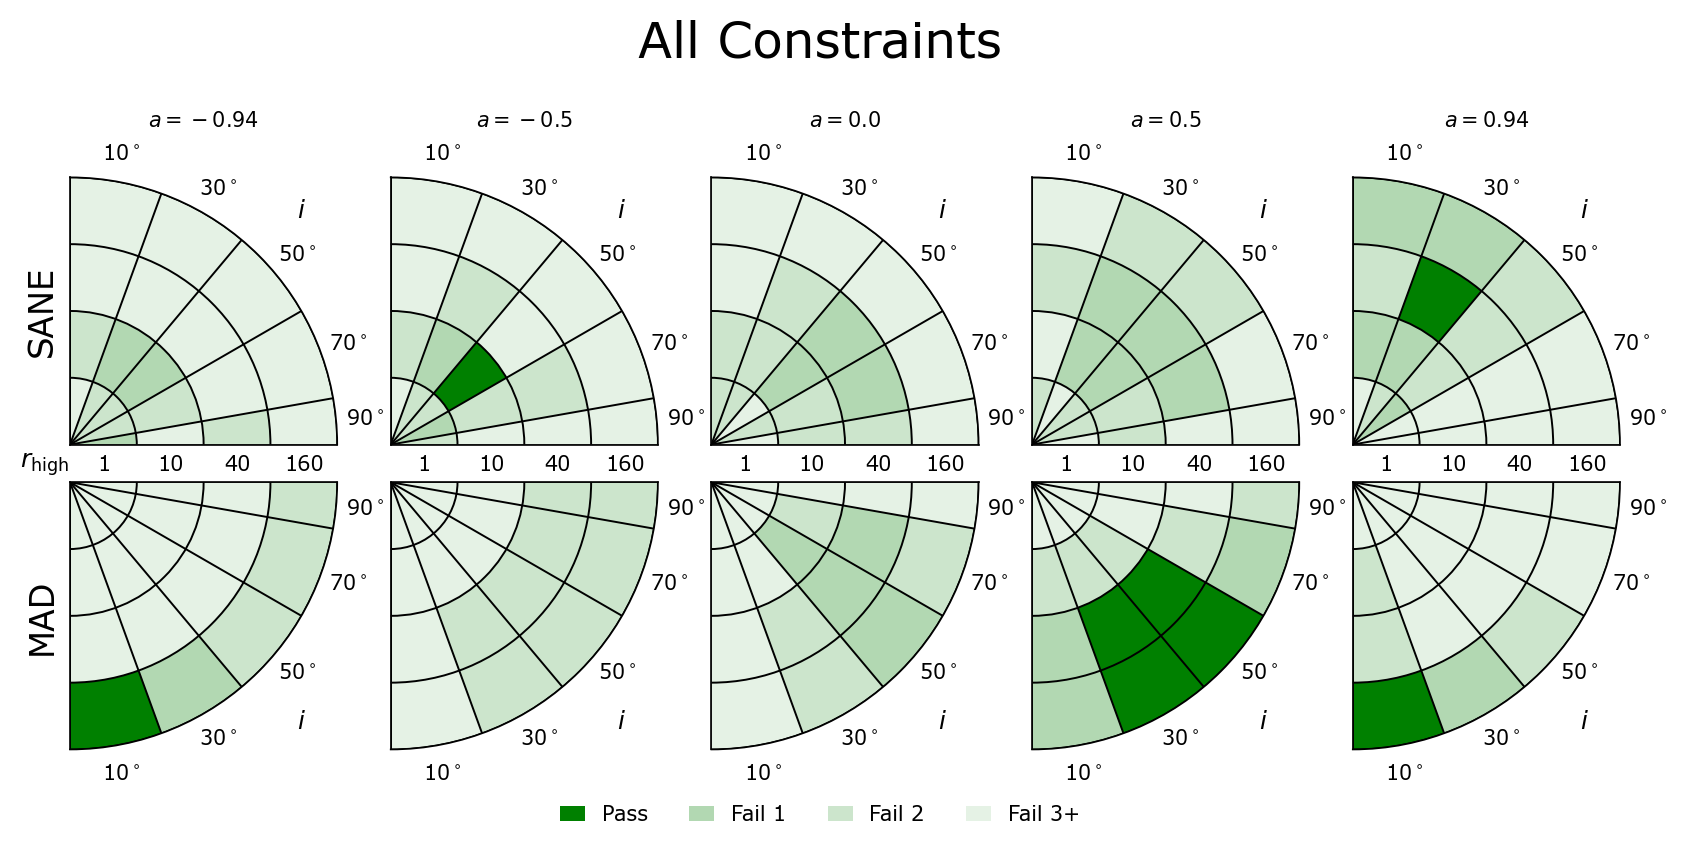
\includegraphics[width=\textwidth]{./figures/All_Constraints.png}
  \caption{Combined EHT and non-EHT constraints.}
  \label{fig:all_cuts}
\end{figure*}

Variability, when included in the constraint map, would eliminate all thermal models.  Although a few models pass the variability constraints alone this does not mean that we should regard them as favored, since we expect to eliminate at least a couple of models incorrectly when using a $1\%$ cut for $200$ models.

% this is now moved to appendix as discussed on Thursday Dec 9 2021 among coordinators
% %------------------------------------------------------------------------------
% \subsubsection{Inter-Model Comparison: $\Rh$ Thermal Models}

% % note: passfail tables are consistently, e.g., tab:illinoisPF or tab:VKhamrPF

% \subsubsubsection{Frankfurt Thermal $\Rh$ Models}

% As can be seen in Table \ref{tab:GRMHDmodels} the thermal models have been calculated for an identical parameter space from two different codes, namely KHARMA and BHAC for the GRMHD simulations and iPOLE and BHOSS for the GRRT calculations. This allows us for the first time to perform an in depth comparison between the different numerical methods used in this work in addition to the EHTC code comparison projects \citep{2019ApJS..243...26P,2020ApJ...897..148G}.

% \begin{figure*}
%   \centering
%   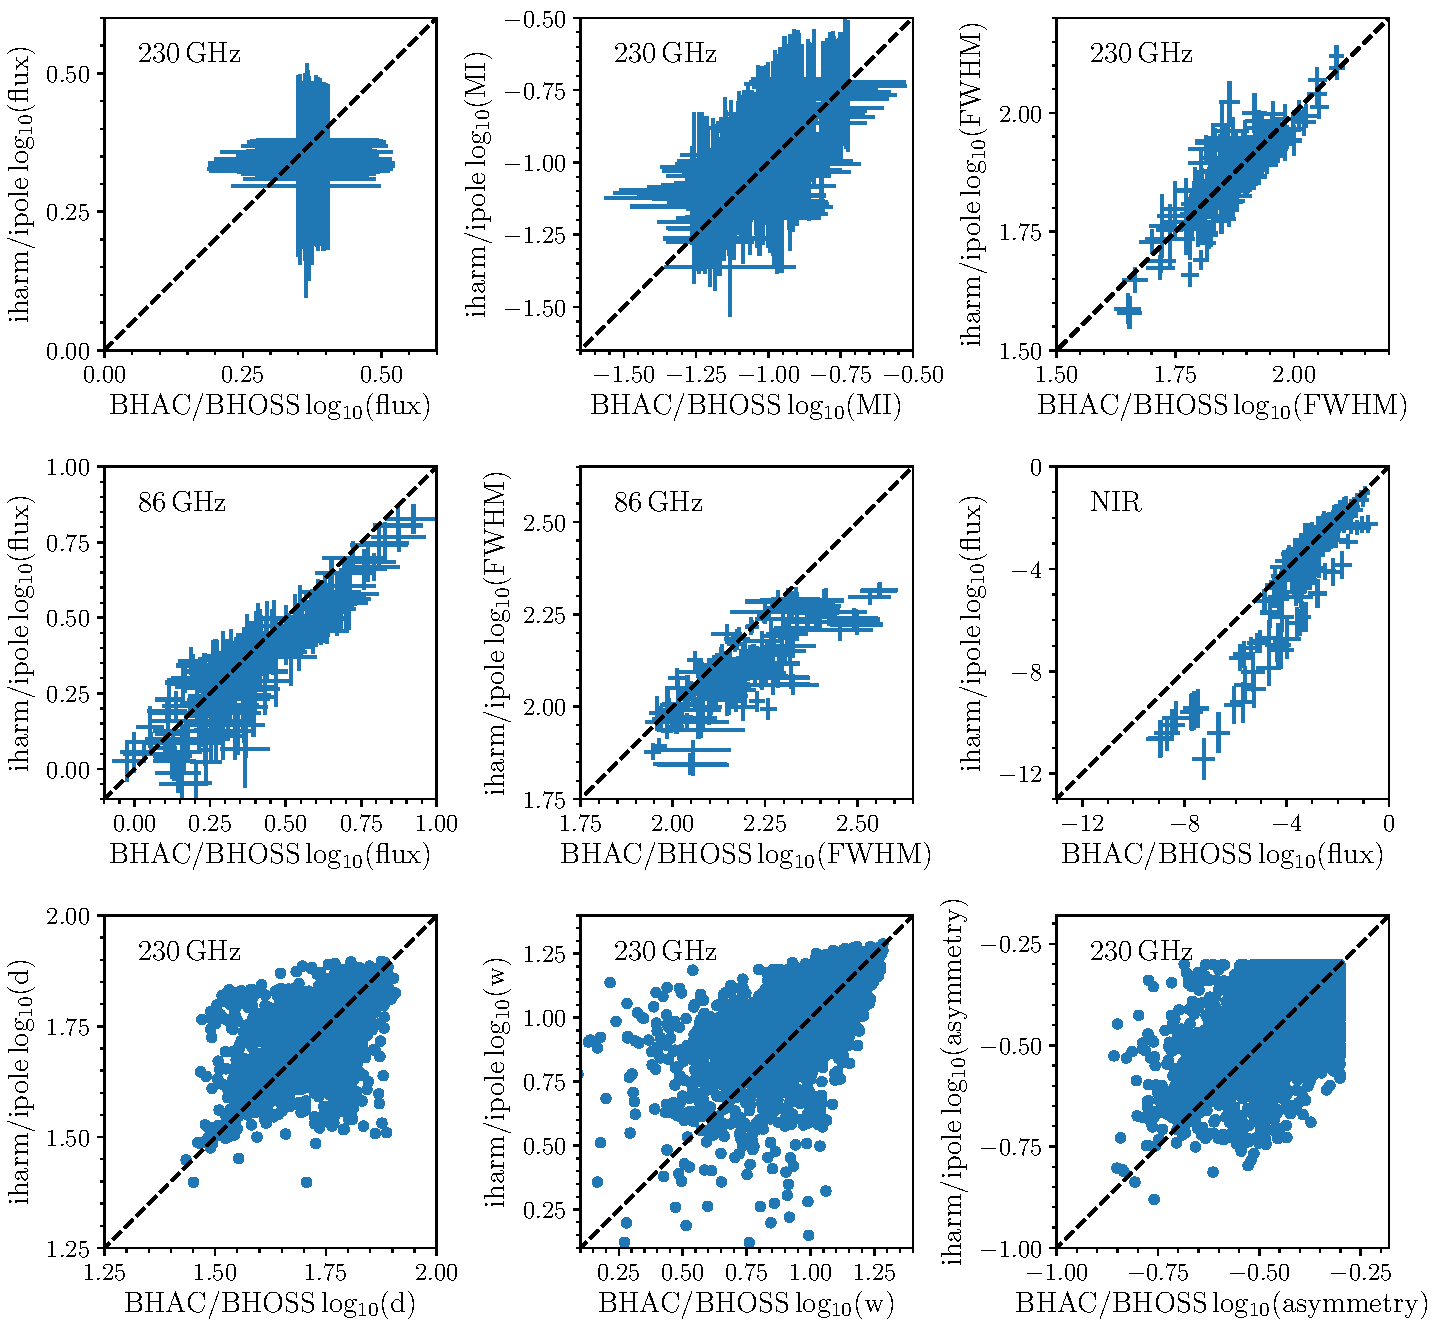
\includegraphics[width=0.8\textwidth]{./figures/BHAC_iharm_correlation}
%   \caption{Correlation between BHAC and KHARMA models for 9 model constraints.  The horizontal axis is the constraint value from \bhac/\bhoss, and the vertical axis shows the constraint value from \kharma/\ipole.  Each point corresponds to a single model, with the width of the distribution shown by the error bars.  See text for details.}
%   \label{fig:modelcorrelation}
% \end{figure*}

% In Figure \ref{fig:modelcorrelation} we show the correlation between the thermal KHARMA and BHAC models for constraints where we have predictions from both models.

% The top row shows from left to right the 230\,GHz flux density, the 230\,GHz modulation index, MI, computed for a time window of 3 hours, and the 230\,GHz image size obtained from image moments. Since we normalise the 230\,GHz images to an average flux of 2.4\,Jy within a time window of 5000\,M (corresponds to 28.5 h for SgrA a mass of $4.14\times 10^6\,\msun$), the scatter around this values is small. The deviation from an ideal correlation reflects the precision and number of GRMHD snapshots included during normalization procedure.

% The correlation in the 3\,hour modulation index spreads over $\Delta \mi{3}=0.75$ which serves as a measure of intra-code ( e.g., MAD vs. SANE accretion) and inter-code (BHAC vs. KHARMA) differences. Despite these differences the models show a strong correlation throughout the investigated models and parameter space.

% We found a strong correlation between models and codes for the image size computed from image moments, i.e. second moments analysis.

% \cfg{This may change if we recompute the major axis, etc., for the IL 86 GHz large fov images}
% The middle row presents the correlation plots for the 86\,GHz flux density (left), the 86\,GHz image size using second moments (middle) and the NIR flux (right). The 86\,GHz flux and 86\,GHz image size exhibit a shift toward larger values for the BHAC models. This difference can be explained by the larger field of view used for the BHAC models at 86\,GHz during the radiative transfer calculations. Thus, more extended structure and therefore a larger total flux is included in the BHAC models. This affects mainly models with large inclinations $i\geq70^\circ$ and jet dominated emission models ($\rm{R}_{\rm high}\geq 40$).

% The NIR fluxes show a tight correlation over four orders of magnitude and systematically larger flux for the BHAC models for low NIR fluxes ($\log_{10}(NIR)<-7$). These fluxes are far below the NIR constraints of $\sim 1mJy$, and therefore they do not affect the passing or failing of the models. In the thermal models the NIR flux is generated from the tail of the electron distribution function and is thus very sensitive to the electron temperature. Small differences in the distribution and value of the electron temperature between the two codes explain the observed de-correlation at very low NIR flux.

% The correlation between models for the m-ring parameters is presented in the third row of Fig.~\ref{fig:modelcorrelation}. The correlation of the diameter of the m-ring is plotted in the left panel. The spread covers nearly the same extent as the 230\,GHz image size (top row, right panel) however the scatter in the correlation is larger.  The same is true for the width of the m-ring (middle panel in the last row of Fig.~\ref{fig:modelcorrelation}). Compared to the diameter and width of the m-ring, the asymmetry of the m-ring is less correlated (right panel). Notice that horizontal and vertical limits in the asymmetries occur since the parameter hits the boundary of the allowed range.

% The smaller correlation of the m-ring parameters as compared to the other parameters presented in Fig.~\ref{fig:modelcorrelation} is a consequence of the noisy nature of the m-ring fits.  Still, the distributions are quite symmetric under reflection across the diagonal, so the models are at least not biased with respect to each other.  Notice also that these plots do not capture all the information that is contained in the distribution of m-ring parameters, just the central value.

% We find ourselves somewhat surprised by the strength of the correlations seen in Figure \ref{fig:modelcorrelation}.  The range of each constraint is significantly larger than the width of the correlation, so the variations between models are real, detectable, and reproducible with independent codes.  The question of the origin of the systematic offsets between models for some constraints (for example, in the NIR) is interesting but beyond the scope of this paper.

% \subsubsubsection{\hamr Models}

% %\note{Doosoo, Koushik to write here about HAMR thermal models.}
% Along the KHARMA/iPOLE and BHAC/BHOSS models, we produced a set of thermal models out to $35,000\tg$ using the GRMHD code H-AMR and the GRRT code BHOSS (see Table~\ref{tab:GRMHDmodels}). These models consider a gas adiabatic index of $\Gamma_{\rm ad}=5/3$ for the SANE models and $\Gamma_{\rm ad}=13/9$ for the MAD models (Table~\ref{tab:radiativemodels}), allowing us to understand how sensitive the images are to the GRMHD fluid properties, in addition to code numerics.

% We are glad to note that overall, the H-AMR/BHOSS thermal eDF images perform similarly to the KHARMA/iPOLE and BHAC/BHOSS models. \kc{needs verification from Michi}

% \kc{is the plan to do H-AMR and KHARMA correlations similar to figure 18?}

%\subsubsubsection{\koral Long Models}
% moved up to variability section
% We have also considered a set of thermal, $\Rh$, MAD models run with the \koral code out to $\sim 100,000\tg$.  These models permit us to assess the importance of integration time for application of the constraints.  They permit us to obtain more accurate distributions for the constraint quantites, and to assess whether the constraints evolve from the beginning to end of the integrations. We do not see evidence for evolution in the \koral  model set (a full pass/fail table is given in Appendix \ref{app:tables}, Table~\ref{tab:koralPF}). The \koral pass/fail results are similar to those for comparable models in the \kharma thermal model set. Moreover the constraints measured at the beginning of the evolution are similar to those measured at the end.

%------------------------------------------------------------------------------
%\subsubsection{Critical Beta Model}

Finally, the $\Rh$ eDF model has been the default parameterization used to span the uncertainties in emitting particle thermodynamics in EHT analyses. The $\Rh$ models  are compatible with the well-motivated turbulent plasma heating ADAF models of \cite{1999ApJ...520..248Q} in asymptotic behavior of electron-to-total heating ratio as a function of plasma $\beta$. There is, however, a vast function space of possible alternative parameterizations. Here we have also considered the Critical Beta model \cite{2020MNRAS.493.1404A}, which sets $T_e = f (T_e + T_i) \exp(-\beta/\beta_c)$.  The model is motivated by the observation that when the transition between electron heating domination and proton heating domination is smoothed (controlled by increasing exponent parameter $\beta_c$), the 230 GHz emitting region profile tends to be less coronally dominated and more compact and asymmetric. This is a consequence, when fixing synthetic image flux, of higher critical beta values shifting the locus of electrons dominating the emission profile towards the colder, higher density equatorial inflow.  We consider only a single point in the critical beta parameter space, with $f = \beta_c = 1$. We have applied a subset of tests to the critical beta models (all except X-ray; NIR is calculated with imaging only and therefore does not include Compton scattering).  The full set of results is given in Appendix~\ref{app:tables}, Table~\ref{tab:betacritPF}. All Critical beta models with high inclinations fail EHT constraints, which is consistent with our main conclusion about the thermal models. We also find that all critical beta models fail all considered non-EHT constraints.


% CFG: we shouldn't report preliminary indications here
%A second motivation is that there are preliminary indications that the exponential electron cooling in the Critical Beta Model suppressed the SANE bremsstrahlung spectral component allowing more to pass the X-ray constraint.

%==============================================================================

\subsection{Nonthermal, Aligned Models}

%\note{Koushik to write here about powerlaw nonthermal HAMR models.  Define a subsection, describe the results and how they differ from the thermal results.][Maybe add Tomohisa's models here as well.] [by including power-law, we see this and that change (only include significant changes from the thermal models)}

So far we have assumed a Maxwell-J{\"u}ttner distribution function that describes a thermal population of electrons. Next we assume that these electrons are accelerated to a non-thermal tail. We model such the energy distribution of such a population of electrons using either a mixed thermal-powerlaw eDF or a pure/mixed kappa eDF. Similar to the thermal models, the accretion rates of all model sets in this section are normalized such that the time-averaged 230\,GHz compact flux is 2.4 Jy over 5,000M. 

\subsubsection{Thermal Plus Constant power-law models with $p_\mathrm{pl} = 4$}

In this section, we employ a hybrid thermal/power-law tail distribution using \hamr/\bhoss, and assume a power-law index of $p=4$ with a constant non-thermal acceleration efficiency $\epsilon=n_{\rm e, power-law}/n_{\rm e, thermal}=0.1$. Following the method given in \citet{Chatterjee2021}, the power-law tail is stitched to the thermal core by choosing the minimum Lorentz factor limit of the power-law $\gamma_{\rm min}$ to be at the peak of the Maxwellian component. The maximum limit of the power-law is taken to $10^5 \gamma_{\rm min}$. Further, we note that the normalization value for the accretion rate is slightly smaller than that of the corresponding \hamr/\bhoss thermal models, suggesting that the power-law emission contributes to the 230\,GHz total intensity.

\subsubsubsection{230\,GHz VLBI pre-image size}

Hybrid thermal/power-law models have similar 230\,GHz VLBI pre-image sizes to their purely thermal counterparts. This is because the power-law index is large enough 

\subsubsubsection{86\,GHz flux} 

In general, the $R_{\rm high}=1$ models produce too much 86\,GHz flux. Since the lower limit of the power-law $\gamma_{\rm min}$ is directly affected by the local electron temperature, the highest energy electrons are located in the jet sheath where the ion and electron temperatures are similar, i.e. $T_i\approx T_e$. Indeed this is why SANE models produce more 86\,GHz flux when non-thermal electrons are introduced, especially at larger $R_{\rm high}$ values. On the other hand, MAD pure thermal and mixed thermal/non-thermal models behave similarly as the bulk of the emission is produced in the inner disk.

\subsubsubsection{86\,GHz image size} 



\subsubsubsection{NIR constraints}

The addition of the power-law tail primarily increases the flux in the NIR and thus, the NIR GRAVITY flux of 1.0 mJy could provide a constraint on the power-law index and the acceleration efficiency. In brief, $R_{\rm high}=1$ and $40$ MAD models are ruled out by the NIR constraint.

\subsubsubsection{ALMA Light curves}
\subsubsubsection{m-ring}

\note{Razi to write here about variable kappa models.  Define a subsection, describe the results and how they differ from the thermal results.}\kc{might be better to move this to 4.2.3 along with bhac/bhoss results}

\note{Christian to write here about constant kappa models.  Define a subsection, describe the results and how they differ from the thermal results.}\cmf{done}

%------------------------------------------------------------------------------
\subsubsection{Thermal plus Constant kappa models $\kappa=3.5$ with variable efficiency, $\varepsilon(\sigma,\beta)$}

To investigate the effect of mixed thermal/nonthermal distribution functions, we combine a thermal electron distribution function with a kappa electron distribution with $\kappa=3.5$. The value of $\kappa=3.5$ is motivated from the spectral slope in the NIR during a quiescent state \cmf{add reference here} \kc{suggest to say that the slope is a limit as $\alpha=0.6$ where $F_{\nu}\propto \nu^{\alpha}$ is seen in the flaring state, e.g., Hornstein+2006}.  In addition to the fixed kappa value we assume that the fraction between thermal and non-thermal particles depends on the local plasma properties, e.g, the magnetisation, $\sigma$, and the plasma beta parameter, $\beta_{\rm p}$. Given this assumption we can write the total emissivity as:
\begin{equation}
j_{\nu,\rm{tot}}=(1-\epsilon) j_{\nu,\rm{thermal}} + \epsilon j_{\nu, \kappa},
\label{eq:kappaeff}
\end{equation}
where the nonthermal efficiency $\epsilon( \varepsilon, \beta, \sigma)$ is
\begin{equation}
    \epsilon(\varepsilon,\beta,\sigma)=\varepsilon\,
    \left[1 - e^{-\beta_{\rm p}^{-2}}\right]
    \left[1-e^{-(\sigma/\sigma_{\rm min})^2}\right].
    \label{eq:efficiencybetasigma}
\end{equation}
Evidently the nonthermal emissivity is non-negligible only when $\beta_p \lesssim 1$ and $\sigma \gtrsim \sigma_{\rm min}$.  We fix $\sigma_{\rm min}=0.01$ and vary the base efficiency, $\varepsilon$, between 0.05, 0.1 and 0.2. For each base efficiency we generate a set of models spanning the same parameter space as the thermal models (see Table \ref{tab:radiativemodels} for details). For each model we iterate the mass accretion rate to obtain an average flux of 2.4\,Jy at 230\,GHz across a time interval of 5000\,M. In order to explore several values of $\varepsilon$ efficiently we increased the model snapshot cadence to 50\,M. This allows us to keep the numerical costs for this parameter sweep low while still being within the correlation time of the GRMHD simulations.
%($t_{\rm corr}\approx 50-100\,M$) \cmf{ do we have reference for this? So far this result is not published, maybe Boris paper?}.
% CFG: this is mentioned earlier in the paper and also implicit, but not actually calculated, in Boris's paper.  Let us not specify a correlation time here, so that we don't set the correlation time in multiple places.

An example of the distribution of the efficiency can be seen in the right half of  Fig. \ref{fig:varepsilon}. The efficiency quickly $\epsilon=0$ within the disk region while within the jet the efficiency reaches the defined base-efficiency. Thus (and as usual removing emission at $\sigma > \sigma_{\rm cut}=1$) the non-thermal particles are mainly located in jet sheath.

\begin{figure}[t!]
  \centering
  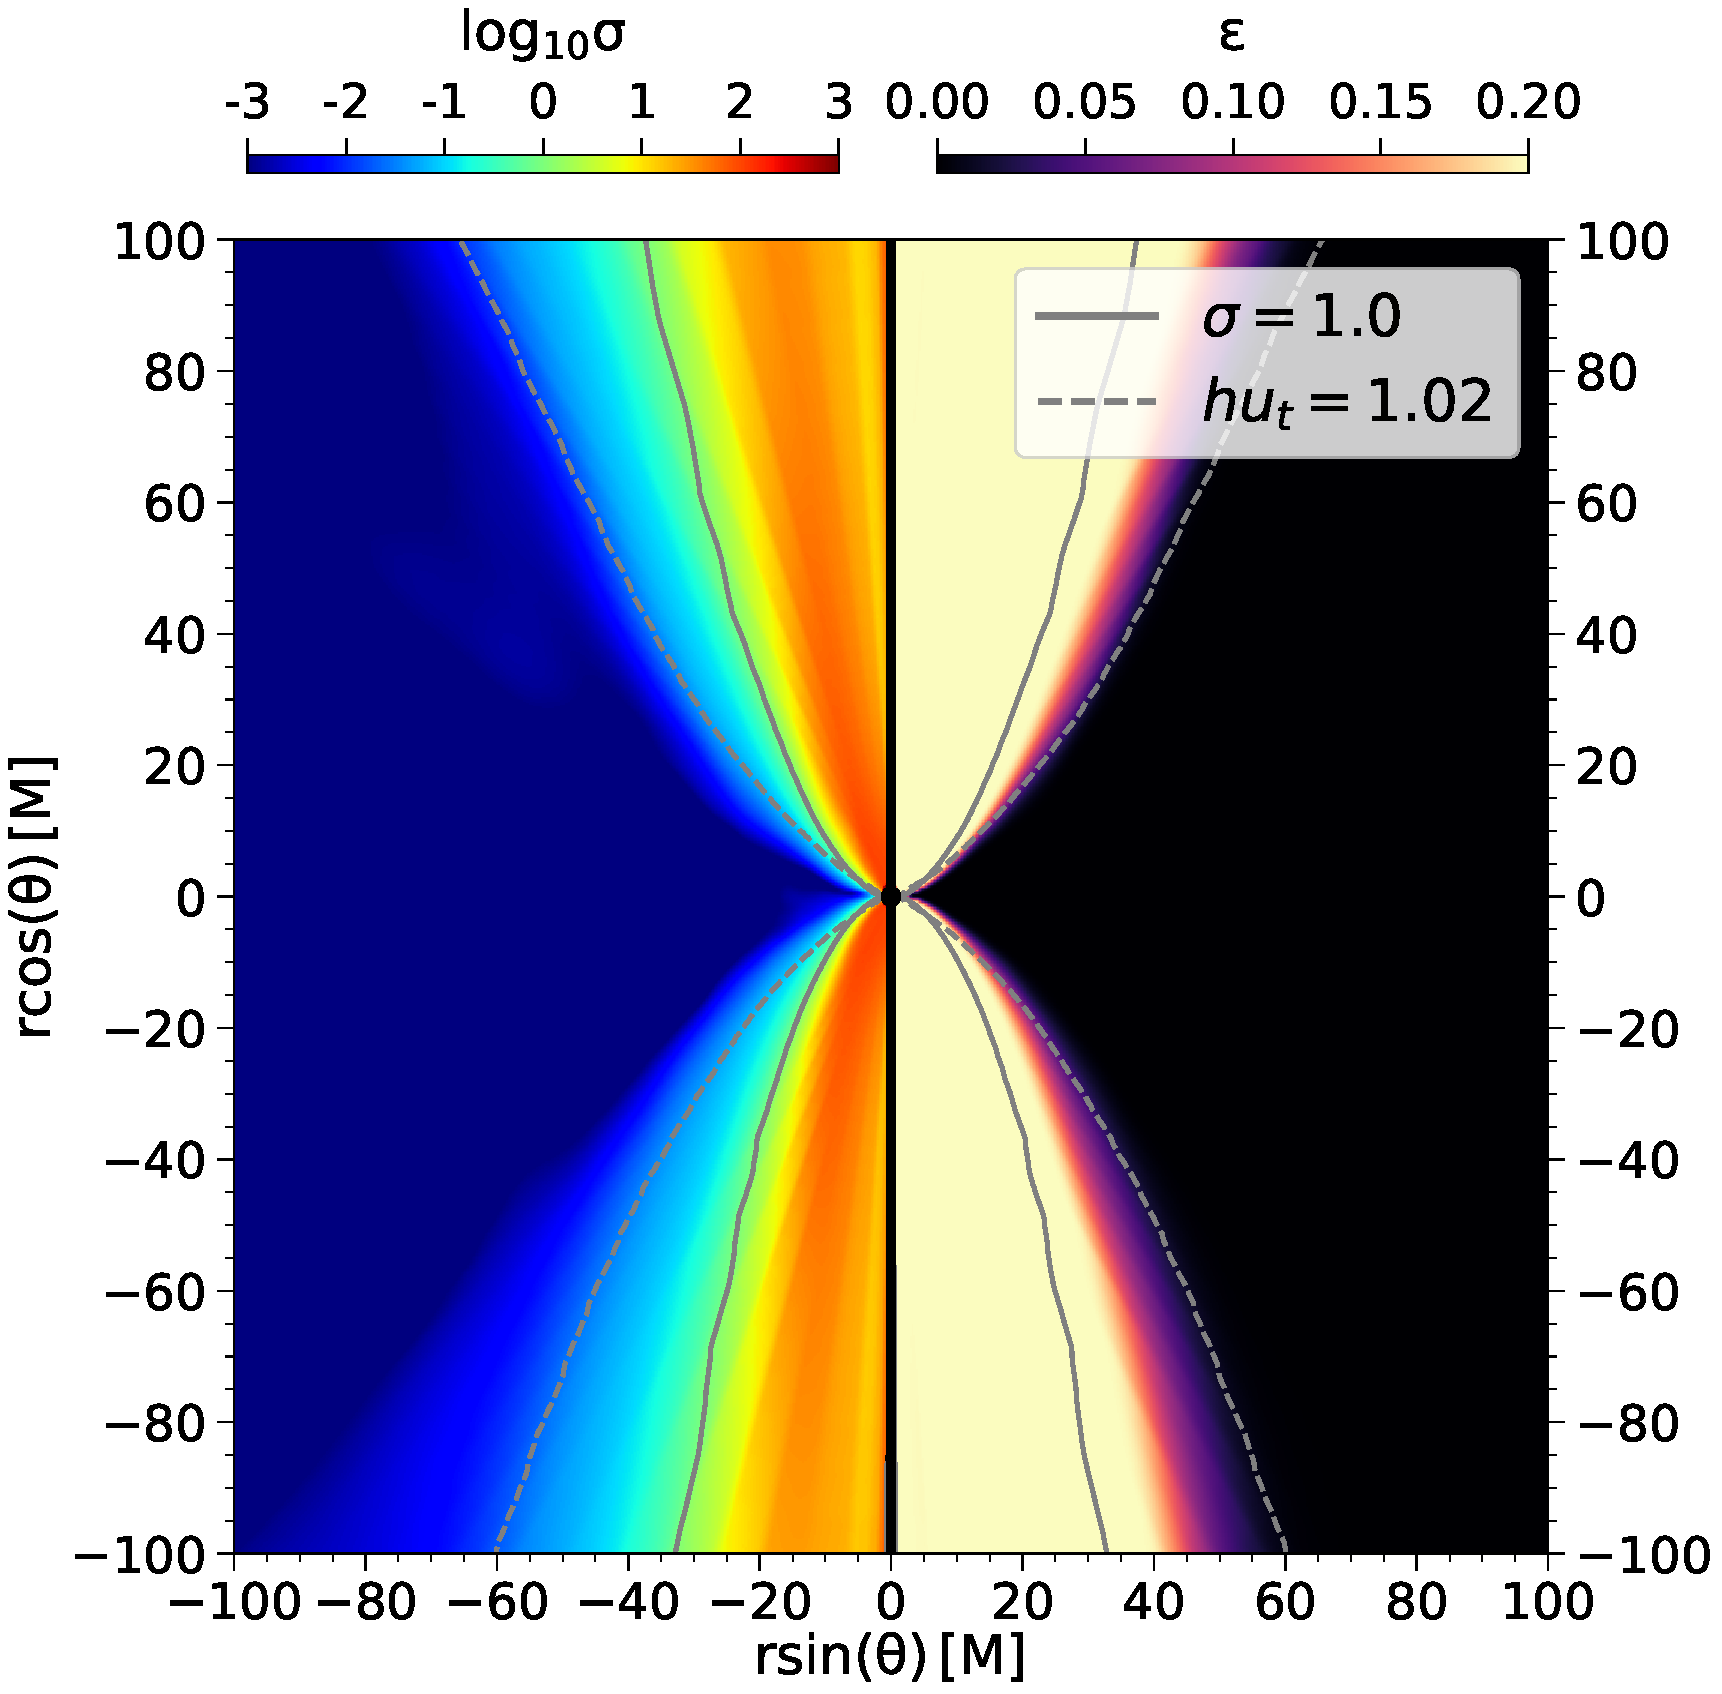
\includegraphics[width=\columnwidth]{./figures/GRMHDphiavera0.94sigmaeta.pdf}
  \caption{Time and azimuthal averaged distribution of the magnetization, $\sigma$ (left half) and the efficiency, $\epsilon(\varepsilon,\beta,\sigma)$ using $\varepsilon=0.2 $ for a \bhac MAD GRMHD simulation with $\abh=0.94$. The solid gray line corresponds to $\sigma=1$ and the dashed line indicates out-flowing plasma via the Bernoulli parameter ($-h u_{t}>1.02$).
  \ckc{Should we move this figure to the model section, as a way to demonstrate how the GRMHD and eDF look like?}}
  \label{fig:varepsilon}
\end{figure}

In the following we will elaborate on the impact of adding non-thermal particles via the kappa electron distribution with fixed kappa value ($\kappa=3.5$) and three different base efficiencies $\varepsilon=$0.05, 0.1 and 0.2 on the observational constraints listed in Section~\ref{subsec:thermal}.

%..............................................................................
\subsubsubsection{230\,GHz VLBI pre-image size}

The addition of non-thermal particles produces almost undetectable changes in the 230\,GHz VLBI pre-image sizes for the MAD models and a minor effect for the SANE models.

In the SANE case only models with $\Rh>40$ exhibit a minor increase in the source size where we see a monotonic increase of the source size with inclination. This effect can be understood if we consider that the bulk of the emission in all cases considered here is still produced by the thermal electron distribution, with temperature set by the $\Rh$ prescription.  An increase in $\Rh$ suppresses the emission from particles in the disk (by decreasing the electron temperature) and thus enhances emission from jet.  Since most the non-thermal particles are located in the sheath of the jet their impact on the source size is largest if the bulk of the thermal emission is also produced there.

% CFG: this is confusing.  is it needed?
%In addition the thermal synchrotron emissivity decreases at high frequency as $j_{\nu}\propto \exp{\left(-(\nu/\nu_c)^{1/3} \right)}$ while for the kappa distribution as $j_{\nu}\propto \nu^{-(\kappa -2)/2}$. This implies that for the same electron temperature the non-thermal flux is compared to a thermal one higher and thus leads to a more extended jet structure for the models including non-thermal particles.

In the MAD case, independent of the choice of $\Rh$ the emission is mostly produced in the disk region (see \citetalias{M87PaperV} and Fig.~8 in \citet{Wong_2022} for a 3-D rendering). Increasing $\Rh$ will not push the emission region into the jet where the non-thermal particles are located and thus their contribution to the total emission structure is negligible.

%..............................................................................
\subsubsubsection{86\,GHz flux}

The 86\,GHz GMVA+ALMA observations
%GMVA+ALMA observations at 86\,GHz \cite{2021ApJ...915...99I} \monika{we can skip reference here, there is only one 86 GHz we talk about in this paper}
probe a larger field of view than the 230\,GHz EHT observations, so we increased the field of view for the 86\,GHz to 800\,$\rm{\mu as}$ during the radiative transfer calculations. Again the non-thermal particles are mainly located in the jet sheath and thus the increased field of view ensures that no extended flux is missing during the comparison with the 86\,GHz observations.

The 86\,GHz for both SANE and MAD models flux is not affected by the addition of non-thermal particles. In case of the SANE models the edges of the 86\,GHz flux distribution are slightly shifted in the case of $\Rh>40$. However, including non-thermal particles even with the highest base efficiency $\varepsilon=0.2$ does not change the scoring of a model, i.e., a thermal-only model which full-fills the 86\,GHz constrain is still accepted if non-thermal particles are included. This behaviour can be explained by the fact that the bulk of the emission in both accretion models is generated in with a few gravitational radii. Since the non-thermal particles are mainly located in the jet sheath and thei ratio between non-thermal to thermal particles is at most 20\% the contribution of the non-thermal particles to the 86\,GHz flux can be neglected.

%..............................................................................
\subsubsubsection{86\,GHz image size}

The behaviour of the 86\,GHz image size is very similar to the above described 230\,GHz image size: There is no change in image size for the MAD models and only a minor increase in the SANE models for $\Rh>40$. The physical reasons for this behaviour follows the same arguments as in the 230\,GHz VLBI pre-image size.

%..............................................................................
\subsubsubsection{NIR constraints}
As expected, the addition of non-thermal particles via the kappa electron distribution function with variable efficiency has a large influence on the NIR flux for all models independent of the accretion model and the $\Rh$ value. In Fig.~\ref{fig:NIR_kappaepsilon} we compare the distribution of the NIR fluxes for thermal and kappa eDF for a SANE accretion model.

\begin{figure*}
  \centering
  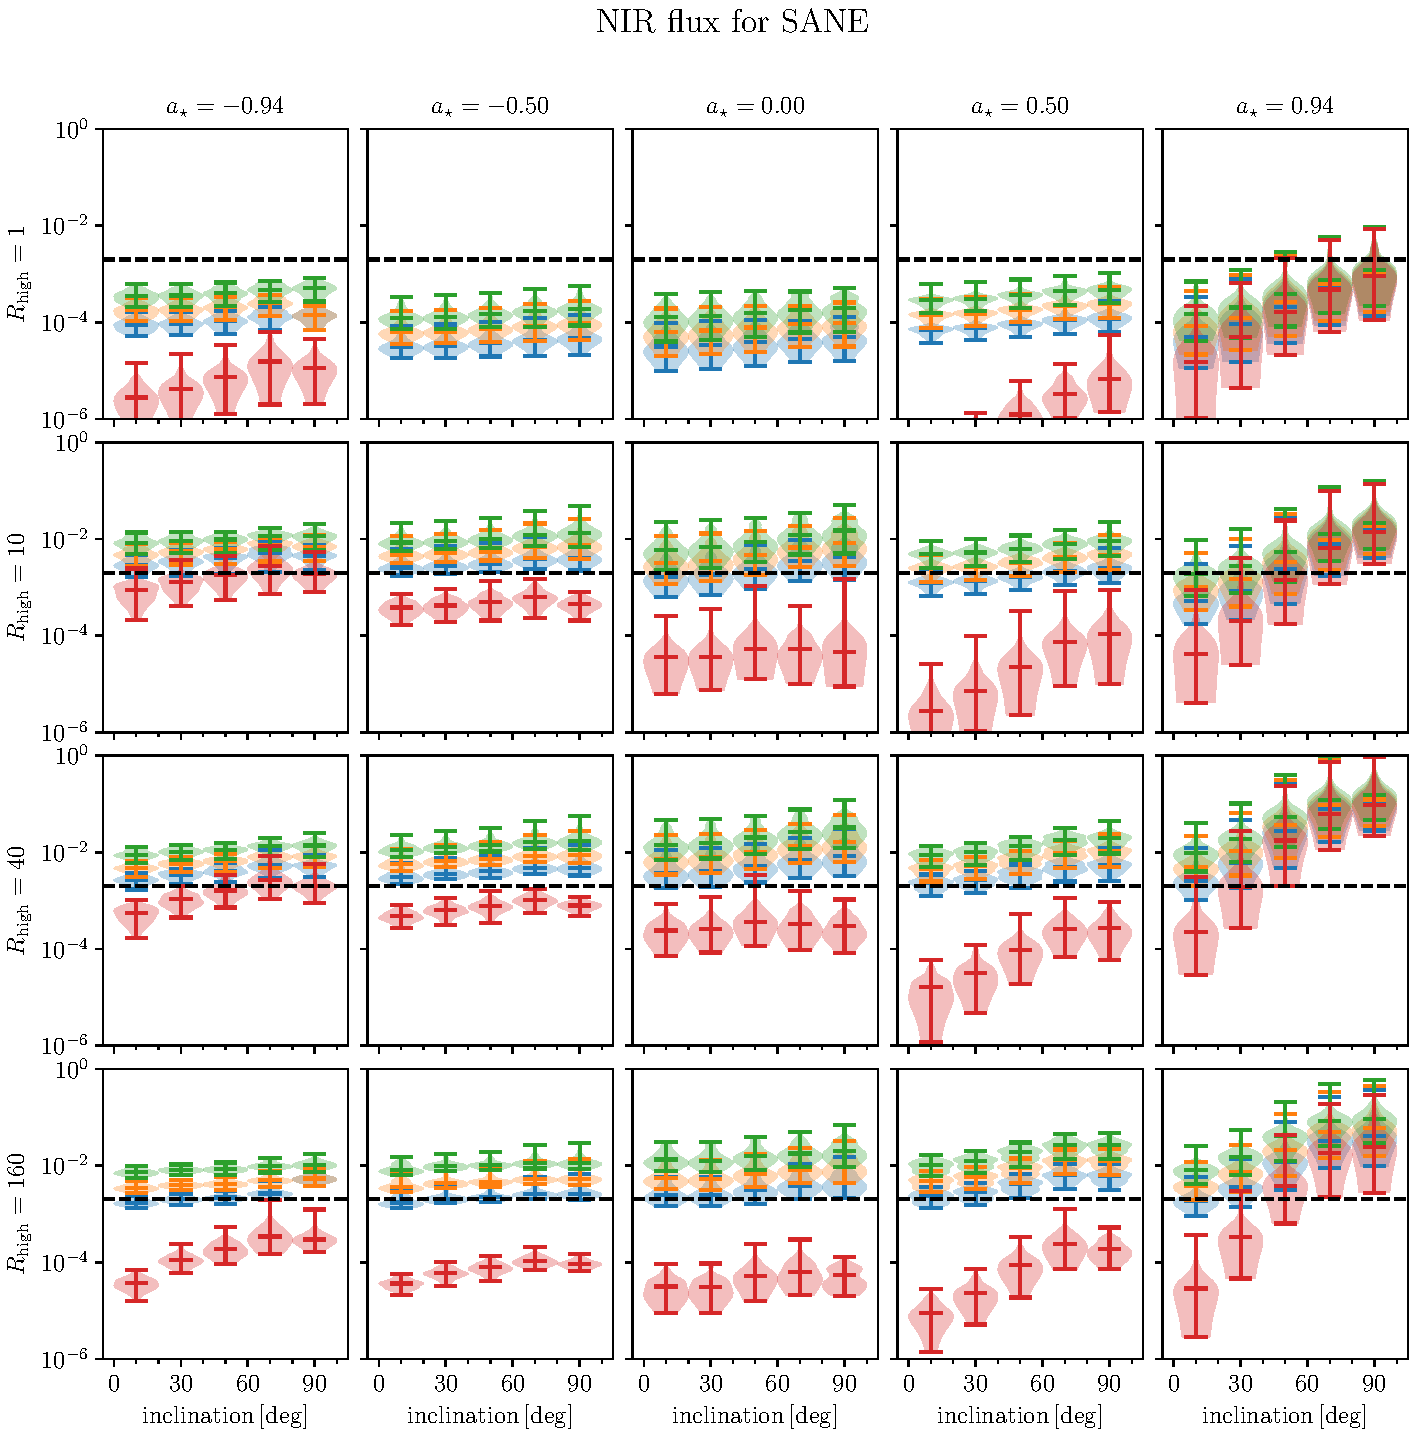
\includegraphics[width=0.8\textwidth]{./figures/SANE_NIR_standard.pdf}
  \caption{Impact of non-thermal electrons on NIR flux constraint. NIR flux distributions are shown for SANE accretion models with thermal and non-thermal eDF with fixed $\kappa=3.4$ and $\epsilon\left(\sigma,\beta,\varepsilon\right)$ defined by Equation~\ref{eq:efficiencybetasigma}. The red violin plots correspond to a thermal eDF, blue, orange and green indicate kappa eDF with $\varepsilon=$0.05,0.1 and 0.2. The horizontal dashed line is the observational constraint.}
  \label{fig:NIR_kappaepsilon}
\end{figure*}

As can be seen in the figure, including non-thermal particles changes the distribution of the NIR fluxes significantly. Except for the $\Rh=1$ models the addition of non-thermal particles even with the lowest base efficiency used in this analysis $\left( \varepsilon=0.05\right)$ leads to a over-production of NIR fluxes. In the case of the MAD models all models over-produce the NIR flux for $\varepsilon=0.05$.

The NIR fluxes are produced by particles in the tail of the distribution function and are therefore are sensitive to slope of the tail. The emissivity for a thermal distribution decreases exponentially $\left(j_{\nu}\propto\exp(-\nu^{1/3})\right)$ while for the kappa distribution it behaves like $j_{\nu}\propto \nu^{-(\kappa-2)/2}$. Thus even at low base efficiencies, $\varepsilon$, the the flux from the kappa distribution in the NIR $\left(\nu\sim 10^{14}\,\rm{Hz}\right)$ is larger than for the thermal eDF.

%..............................................................................
\subsubsubsection{ALMA Light curves}

For the comparison with the ALMA light curves we compute the modulation index for a 3\,hour time window and across the entire simulated time window of 28\,hours (5000\,GM/c$^3$). Similar to the 86\,GHz flux the 230\,GHz flux is mainly produced within a few gravitational radii and thus not affected by the addition of non-thermal particles using Eq. \ref{eq:kappaeff}. As in the previous constraints, the MAD accretion models are insensitive to the addition of non-thermal particles whereas the SANE models show some increased modulation index for $\Rh>40$. However, the distributions for thermal and non-thermal eDF are still largely overlapping.

%..............................................................................
\subsubsubsection{m-ring}

The m-ring fitting is applied to the 230\,GHz images. As mentioned earlier the flux and size of the 230\,GHz images are not affected by the inclusion of non-thermal particles with fixed kappa and variable efficiency. Thus, we do not expect any changes in the distribution of the m-ring parameters.  Applying m-ring fitting to non-thermal models and a detailed comparison with the thermal results confirmed our initial assumption. \cmf{based on the results of Kotaro, who run the m-ring on non-thermal models}

%------------------------------------------------------------------------------
\subsubsection{Variable kappa model $\kappa(\sigma,\beta)$}

%\cfg{could we avod the equation and simply provide a reference and enough detail that someone could reproduce it?}\aco{What about inline equations?}

An alternative procedure for assigning a nonthermal eDF uses the  kappa model \eqref{eq:nonthermaleDF}, and assigns the parameter $w$  and $\kappa$ parameters according to \cite{2018ApJ...862...80B}, who model the effects of particle acceleration in magnetic reconnection based on particle-in-cell simulations: $ \kappa=2.8 +0.7\sigma^{-1/2} + 3.7\sigma^{-0.19}\tanh{(23.4\sigma^{0.26} \beta)}\label{eq:kappa}$
and $w= \frac{ \kappa -3 }{\kappa} \Theta_{\rm e} + \frac{\varepsilon}{2}\left[1+\tanh(r-r_{\rm inj})\right]\, \frac{ \kappa -3 }{6 \kappa} \frac{m_{\rm p}}{m_{\rm e}} \sigma$.
Here $\sigma \equiv B^2/(8\pi\rho c^2)$, $\beta \equiv p_{gas} 8 \pi/B^2$, and $w$ contains a thermal and nonthermal contribution, with the nonthermal contribution defined by the magnetization and nonthermal particle acceleration efficiency $\varepsilon$  \citep{2019A&A...632A...2D, 2021NatAs.tmp..218C}. We set  $\varepsilon=0$ and injection radius $r_{\rm inj}=10r_{g}$ following previous studies.  Nonzero $\varepsilon$ increases the averaged NIR flux by two orders of magnitude as $\varepsilon$ goes from 0 to 1, causing all models to overshoot NIR constraint.  Setting $\varepsilon \ne 0$ also causes the 86GHz flux density to increase around two times as well as the image size \citep{2021arXiv211102518F}. We use the emissivity and absorptivity, computed numerically for the interval $3 < \kappa \le 8$, from  \cite{2016ApJ...822...34P}. For $\kappa > 8$ we substitute a thermal eDF.  We also turn off emission in the jet spine where $\sigma > 1$ (see Figure~\ref{fig:varepsilon}).



%..............................................................................
\subsubsubsection{86\,GHz image size}

The total flux and image size was computed using an extended field of view, $800 \mu as$ motivated in the 86GHz observations. We found that the image size is closely similar to the thermal and variable efficiency models, only different for non-spinning black holes, where we have low magnetized and small jet. As a consequence eDF with variable kappa power-law reduces to thermal distribution and the size of the image is a bit smaller than in thermal case. For $a_{\star}=0$ almost all SANE models pass the size constraint, $R_{\rm high}=1$ we have a bit larger image. For MAD $R_{\rm high}=40$ and $a_{\star}=0.94$, and cases for $R_{\rm high}=160$ and $a_{\star}=0.50$ we have a bit smaller size image than thermal case passing the constraint.

%..............................................................................
\subsubsubsection{86\,GHz flux}

The total flux on overall non-thermal models increases in comparison to thermal models, however, the general results for MAD models do not change. For SANE models with R$_{\rm high}=1$ slightly increases, all of them fail in contrast with thermal models. While for $R_{\rm high}=10,40,80$ and $R_{\rm high}=160$ the flux decreases under the lower bound $1.8 \rm {Jy}$.

%..............................................................................
\subsubsubsection{NIR constraints}

The contribution of non-thermal electrons at the NIR emission produce larger flux in all models, independent on black hole spin, inclination angle or electron temperature. For MAD accretion models with $a_{\star}=0$ and $R_{\rm high}=1$ only small inclination $i=10^{\circ}$ pass the constraint. While models with $R_{\rm high}=10,40$ overshooting GRAVITY mean flux, again for thermal case these models satisfy the constraint. On the other hand, since for non-spinning black hole the jet is no well developed and the magnetization is low, for only  $R_{\rm high}=80$, $a_{\star}=0.5$ and $30^{\circ} \leq i$ survive, similar behavior for $R_{\rm high}=160$ and spins $|a_{\star}|=0.5$.
Larger emission than thermal models excludes SANE models for $R_{\rm high}=10$ and $\abh < 0$ as well as  $R_{\rm high}=40,~80$ and $\abh \leq 0.0$. While even larger NIR flux the models for $R_{\rm high}=160$ are still under the threshold.

%..............................................................................
\subsubsubsection{ALMA Light curves}

We compute the the modulation index  of the light curves of variable kappa models by discretizing the entire window of GRMHD simulations, $\rm 5000\,\tg$ ($\rm 28\,hours$) every $\rm 3\,hour$ (see Table \ref{tab:GRMHDmodels}). Similar to variable efficiency models, the non-thermal particles with variable kappa has not big impact on the flux at 230GHz. The behavior of modulation index and total flux for MAD accretion models are same as thermal, and variable efficiency eDFs. We found sightly high modulation index for $R_{\rm high}=1$ and $30^{\circ} \leq i$ for SANE accretion models, the models for $R_{\rm high}=80$ has same trend as $R_{\rm high}=40$.


%..............................................................................
%\aco{First Draft ... please add missing references ... waiting for calculations with help from Michi, Ben, Ck and Kotaro}\\

\subsubsubsection{m-ring}

...

\subsubsubsection{Null Location}

...

\note{Razi, Angelo, Richard?}
\ckc{Write subsections only if they are different from the thermal models.}

%------------------------------------------------------------------------------
\subsubsection{Summary of Constraints on Non-thermal Models}

The effect of adding non-thermal electrons in a kappa eDF with  $\kappa=3.4$ and variable efficiency via Eq.~\ref{eq:efficiencybetasigma} can be summarised as follows:
\begin{itemize}
    \item The 86\,GHz and 230\,GHz constraints are hardly affected by the addition of non-thermal particles.
    \item Even the lowest base efficiency considered, $\varepsilon=0.05$, leads to an over-production of NIR flux. \cmf{indication that we need very localised regions of non-thermal particle productions and no "global" approach?}
\end{itemize}

\note{Tomohisa to write here about UWABAMI nonthermal power-law models}

\ckc{Write subsections only if they are different from the thermal models.}

%==============================================================================
\subsection{Tilted Models}

\note{Koushik to write here.  Describe the results and how they differ from aligned thermal results.}
\ckc{Write subsections only if they are different from the thermal models.}

In addition to the aligned models, we also consider misaligned, geometrically thick disks around black holes with a spin of $a_*=15/16$ from \citet{Liska2018} and \citet{Chatterjee2020}. While the other models in this paper produce either a SANE or MAD accretion flow, the tilted disk models assume a strongly magnetized non-MAD disk, otherwise known as an INSANE disk. Overall, we incorporate three GRMHD models of differing misalignment angles - $0^{\circ}$, $30^{\circ}$ and $60^{\circ}$. The models show a strongly warped disk and jets due to the Lense-Thirring torque imposed by the black hole frame dragging effect, and thus the disk/jet morphology is non-axisymmetric. Since the inner and the outer disk possess different orientations, it is necessary to specify the coordinate axis of the observer. We chose to align our observer to the outer disk such that at an inclination and azimuth of $90^{\circ}$ and $0^{\circ}$ respectively, we are observing the outer disk edge-on \citep[for more details, see][]{Chatterjee2020}. Note that the jets are always approximately perpendicular in orientation to the disk in these models.

The 230\,GHz pre-image size of edge-on large $R_{\rm high}$ images slightly increases for the tilt-$60^{\circ}$ as compared to the aligned case. This apparent increase in size occurs as the inner jet is warped and creates an extended image. This effect is also seen in the case of the 86\,GHz image size. On the other hand, the 86\,GHz flux constraint results are quite similar between the three tilt models despite the presence of a boosted jet component at large tilt angles. This suggests that, on average, most of the total flux at 230 and 86\,GHz comes from a few gravitational radii from the black hole where the relativistic Doppler boost have comparable values between the in-going accretion flow and the out-flowing jet. However, highly misaligned models are more variable that their aligned counterparts. In tilted disks, accretion occurs via thin plunging streams \citep[e.g.,][]{Fragile2007} where electrons in the shocked flow can be heated to relativistic temperatures \citep[e.g.][]{Dexter2013}, forming local hotspots more easily than in aligned disks, thereby increasing flux variability \citep{Chatterjee2020}.

The nIR flux exceeds the 1.0 mJy limit for all 3 models (except for a few cases, e.g. $R_{\rm high}=160$ models at $10^{\circ}$ inclination), which makes it difficult to favor the aligned case over the tilted one. Further, the presence of misalignment destroys the axisymmetric nature of the accretion flow. The current model set covers a small parameter space in inclination and $R_{\rm high}$ and a thorough exploration of the source azimuthal angle with respect to the observer is left to future studies. 

%==============================================================================
\subsection{Stellar Wind Fed Models}

The accretion models of \cite{2020ApJ...896L...6R, 2020MNRAS.492.3272R, 2018MNRAS.478.3544R} track plasma from  magnetized stellar winds down to the event horizon and provide a self-consistent picture of the origin of both gas and magnetic fields for the accreting plasma in \sgra.  The resulting inflow does not fully circularize, so the models also provide a distinct alternative to the standard models, which {\em assume} that the artificial SANE or MAD initial conditions relax to a astrophysically realizable state for the inner accretion flow.

We consider two versions of the model: one in which the stellar wind magnetization is low ($\beta = 10^6$) and another and a second in which the magnetization is higher ($\beta = 10^2$). $\Rh$ is adjusted until each model has the observed mean flux, with $\Rh = 13$ ($\beta = 10^6$) and $\Rh = 28$ ($\beta = 10^2$).

While both models pass many of the tests, they both fail the m-ring width test, producing a width that is too small.  In addition both fail the 86GHz flux test: the 86GHz flux is too large. All scoring results for this model are given in Appendix~\ref{app:tables}, Table \ref{tab:resslerPF}.

Interestingly both non-EHT and EHT constraints have the power to test the wind-fed model.  We cannot draw a broad conclusion about the viability of wind-fed models, however, as the two models only consider a single spin and a single eDF model.

%==============================================================================
\subsection{Best Bet Models}

\begin{figure*}
  \centering
  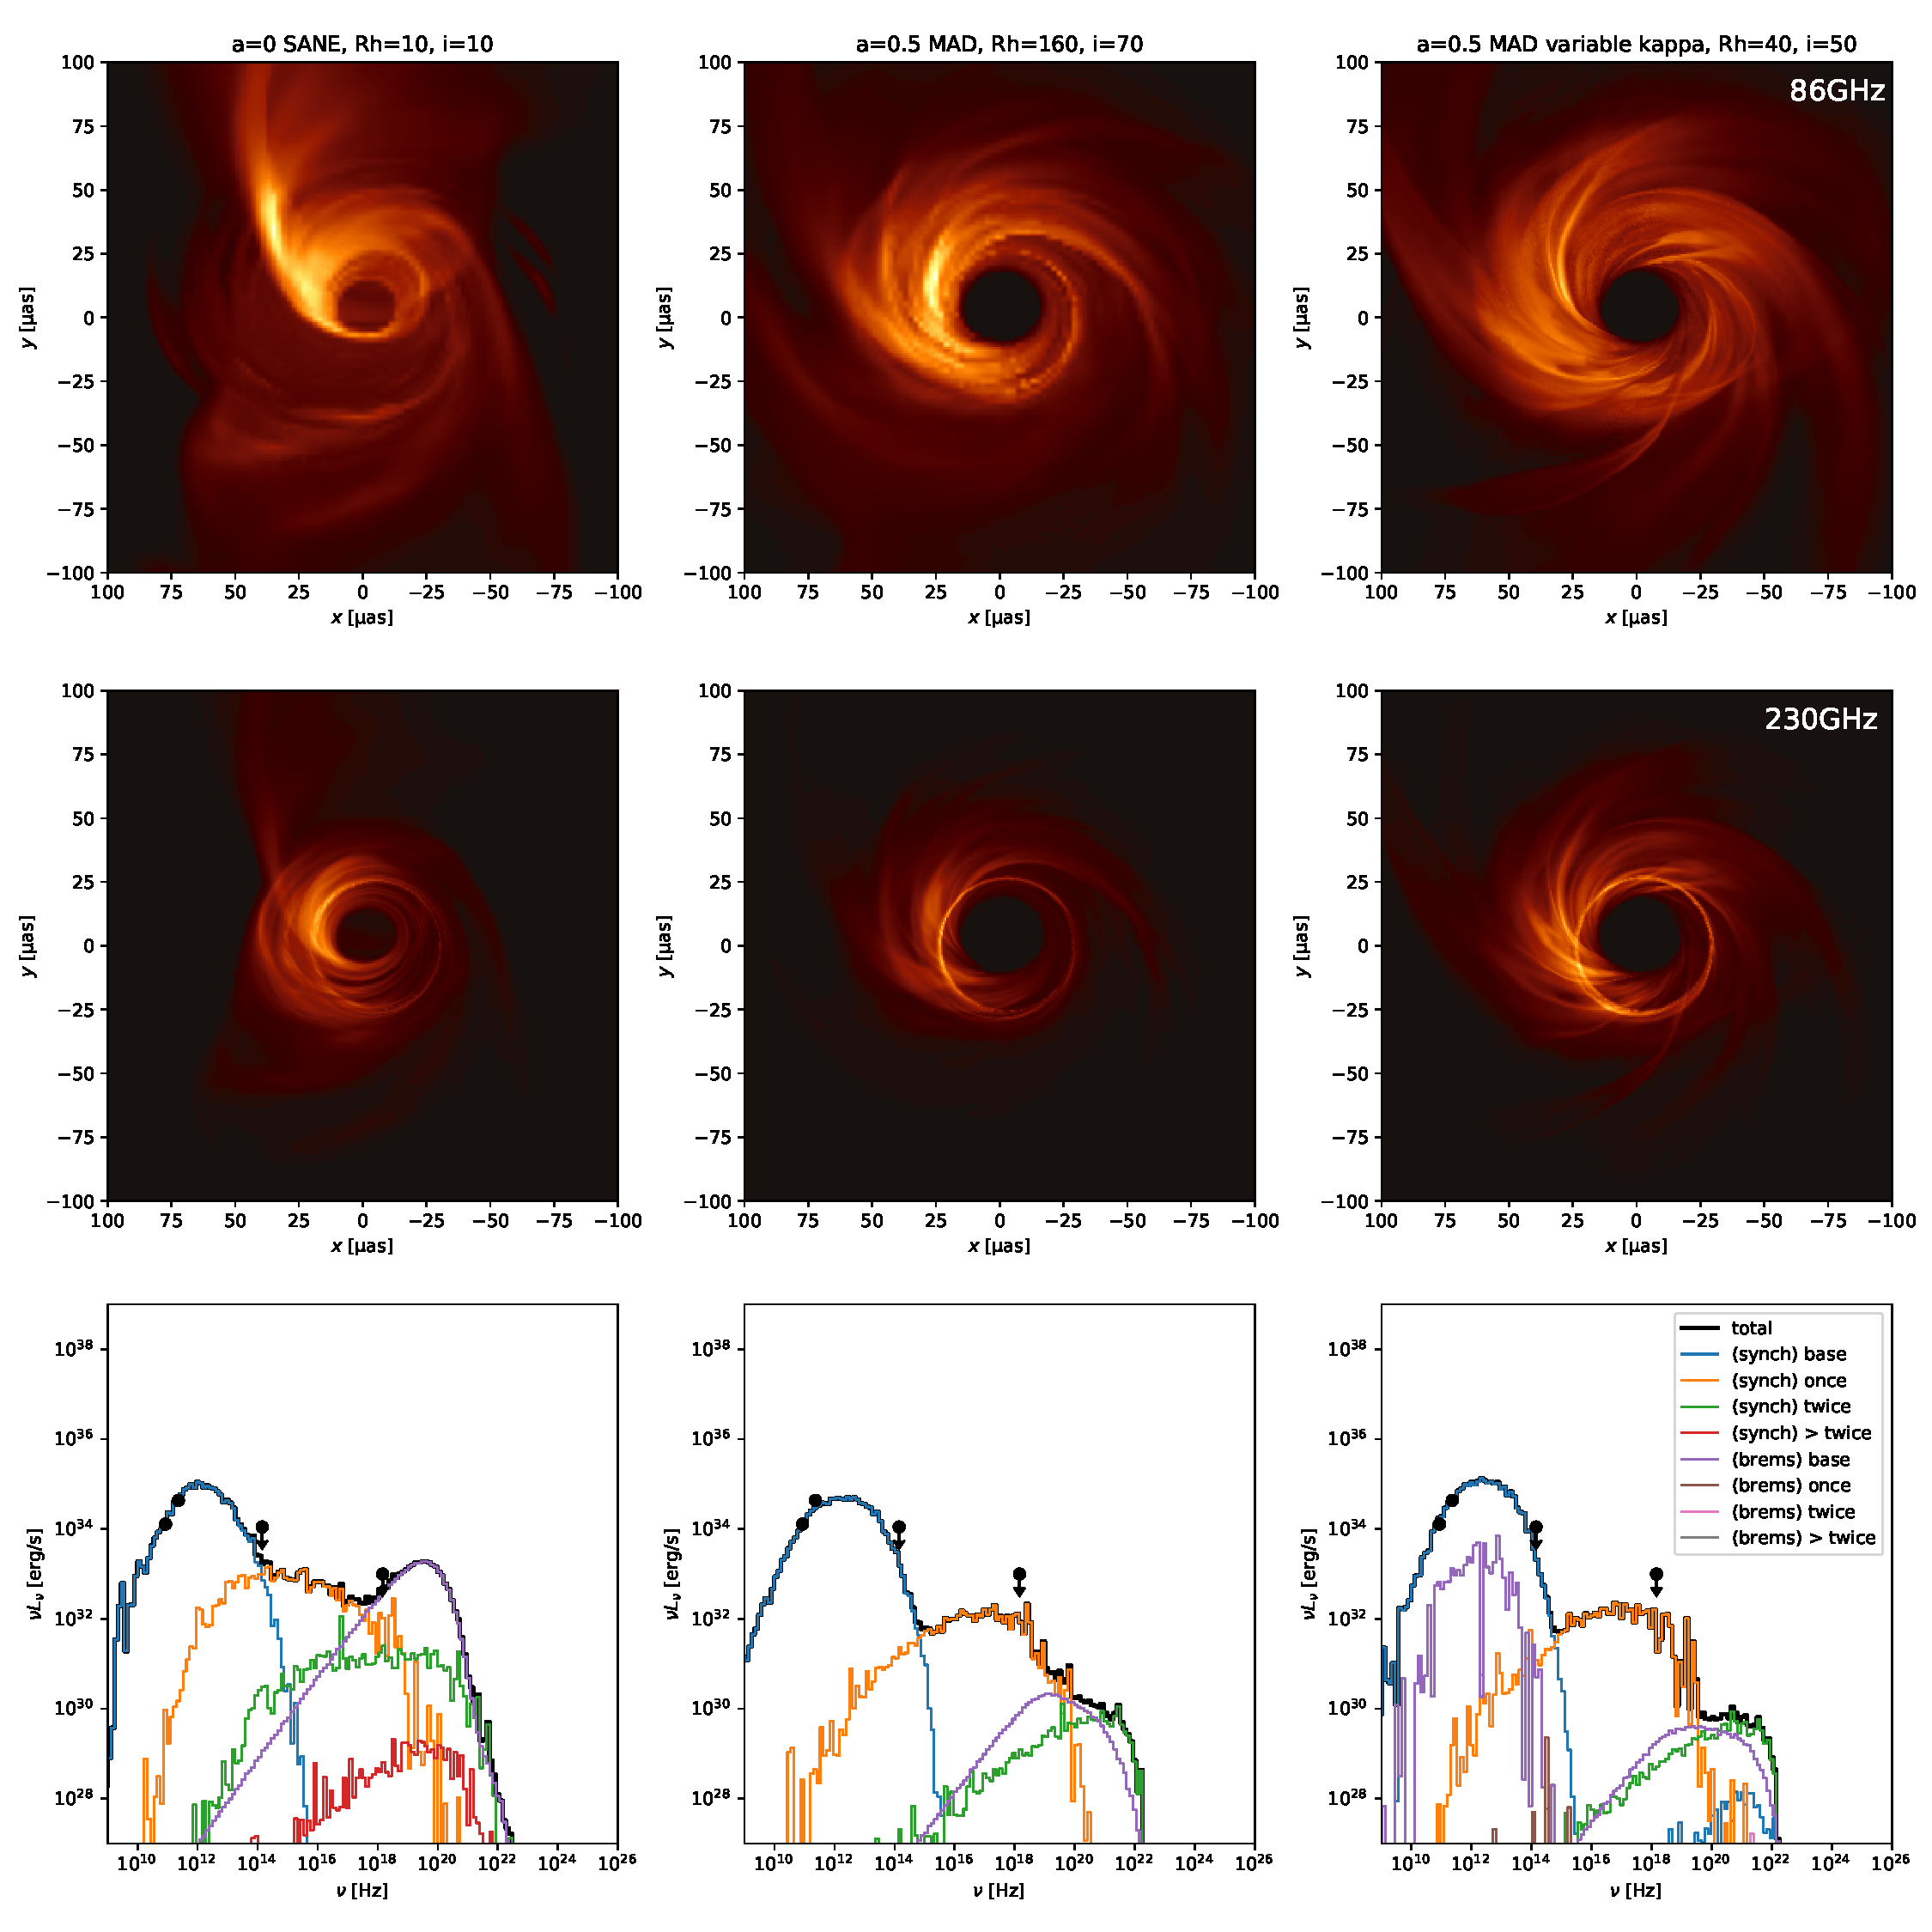
\includegraphics[width=\textwidth]{figures/bestbet.pdf}
  \caption{Best bet models.  Each column corresponds to one best bet model; top row shows 86~GHz image, middle row 230~GHz and the bottom row shows the corresponding multiwavelength broadband SED.} \label{fig:bestbet}
\end{figure*}

We now consider combined constraints, excluding variability, under the hypothesis that (1) there is a missing physical ingredient in the models that would lower variability, but (2) that missing ingredient would not vitiate the model comparison process entirely.  Models are eliminated if they fail any one constraint.

Figure showing combined constraints for thermal models.

Figure showing combined constraints for nonthermal models.

We then inspected the remaining models and selected four best-bet models that approximately span the space of successful models.  \note{Written characterization of remaining models; possibly 3 or 5}

\ckc{CK to work on sample plots, may add extra best bet models upon requests.}


\section{Discussion}\label{sec:discussions}

First comprehensive analysis of Sgr A* including both resolved VLBI data and multiwavelength data.

Discussion organized according to physical parameters of the model.

\note{Avoid figures where possible.}

%==============================================================================
\subsection{MAD, SANE, and Self-Consistent Wind Feeding}

\note{Angelo to provide first draft}

There are clear differences between MAD and SANE models in VLBI data, as well as in the non-VLBI data.

Assessment of Ressler model.  Viable!

%==============================================================================
\subsection{Electron Distribution Function}

\note{Koushik to provide first draft}

Strong constraint on abundance of cold electrons from bremss.  A high density of cold electrons - which would be invisible in synchrotron - are ruled out.  This is in part because at $\Theta_e \equiv k T_e/(m_e c^2) \lesssim 1$, $j_\nu \propto \Theta_e^{-1/2}$ (emission in the x-ray band increases as temperature decreases).  In contrast, for $\Theta_e \gtrsim 1$ electron-electron bremsstrahlung becomes important and $j_\nu \propto \Theta_e^{+1/2}$.

Strong constraint on abundance of hot electrons from NIR.  In particular for

Strong constraint on $T_i/T_e$: models with ion temperature equal to electron temperature fail on several counts.

%==============================================================================
\subsection{Inclination}

\note{Michi to provide first draft}

Strong constraints on inclination from m-ring fitting.

%==============================================================================
\subsection{Position Angle}

Virtually no constraint on position angle [check m-ring fits]

%==============================================================================
\subsection{Black Hole Spin}

Still quite weak constraints on black hole spin.

%==============================================================================
\subsection{Accretion Rate and Outflow Power}

\note{Vedant to provide first draft of thermal section.}

We compute the outflow power in a fashion similar to that in \citet{M87PaperV},

\begin{equation}
    P_{out} = \int_{funnel}d\theta\frac{1}{\Delta t}\int dtd\phi\sqrt{-g}\big(-T^{r}_{t}-\rho u^{r}\big),
\end{equation}

evaluated at $r=100GM/c^{2}$, where $funnel\Rightarrow(\theta<1)\cup(\theta>\pi-1)$. We average the quantity in time $\Delta t$, where $\Delta t$ is the time interval we have considered for our analysis. We also consider only those regions where there is steady outflow, ie. the quantity in the parentheses is positive.

Figure showing accretion rate.

Accretion rate is consistent with earlier analyses.

Models at the highest accretion rate are ruled out by overproduction of x-ray emission.  If our models were in equilibrium over a larger range in radius, bremss from larger radius might increase the x-ray flux and rule out more models.

Figure showing outflow power.

Jet power is surprisingly large.  Where does the power come out in the galactic center?

Dependence on distribution function.

\note{Koushik, Alejandro, Razi}

%==============================================================================
%\subsection{Analytical Accretion Models
%  [Pu, Anantua, Jeter]}
%\label{sec:anamodels}

\subsection{Positrons}

\ckc{Review panel suggested not to include RIAF model.  Please repurpose this section to discuss positrons.  Avoid figures when possible.}

\cite{Broderick2005} devised a canonical model of Sgr A* as a  radiatively inefficient accretion flow (RIAF). Semi-analytic RIAF models implementing  this using the general relativistic ray tracer GRTRANS \citep{2016MNRAS.462..115D} can be found in  \cite{Emami2021}, where  positrons are included using emission modeling motivated in  \cite{Anantua:2019bna}. The Fig. \ref{fig:EmamiRIAF} model from \cite{Emami2021}  shows Stokes maps and polarized spectra of a \cite{Broderick2005} RIAF with plasma $\beta=10$ and 1$\%$ of the emitting particles nonthermal electrons. The near-extremal ($a/M=0.998$) model shown exhibits Doppler boosting asymmetry in a crescent-shaped intensity pattern with a spiral global electric vector polarization angle (EVPA) pattern and polarization preferentially distributed within this region.

The addition of small non-thermal populations of positrons \citep{Anantua:2019bna,Emami2021} tends to: increase overall intensity in jet regions for fixed electron number density; modify the low-frequency spectral slope; cancel the observed intrinsic circular polarization and enhance circular polarization due to Faraday conversion. The last of these positron effects is particularly apparent when comparing declining tails of x-ray spectra of positron-rich versus positron-poor sources, as seen in Fig. \ref{fig:EmamiRIAFSpectra}.

\begin{figure}%[H]
%   \plotone{RIAFSgrAPlaneTscl1Pt5e11beta1Pt0e01fpos0Pt0fNTH1Pt0e-02copy.png}
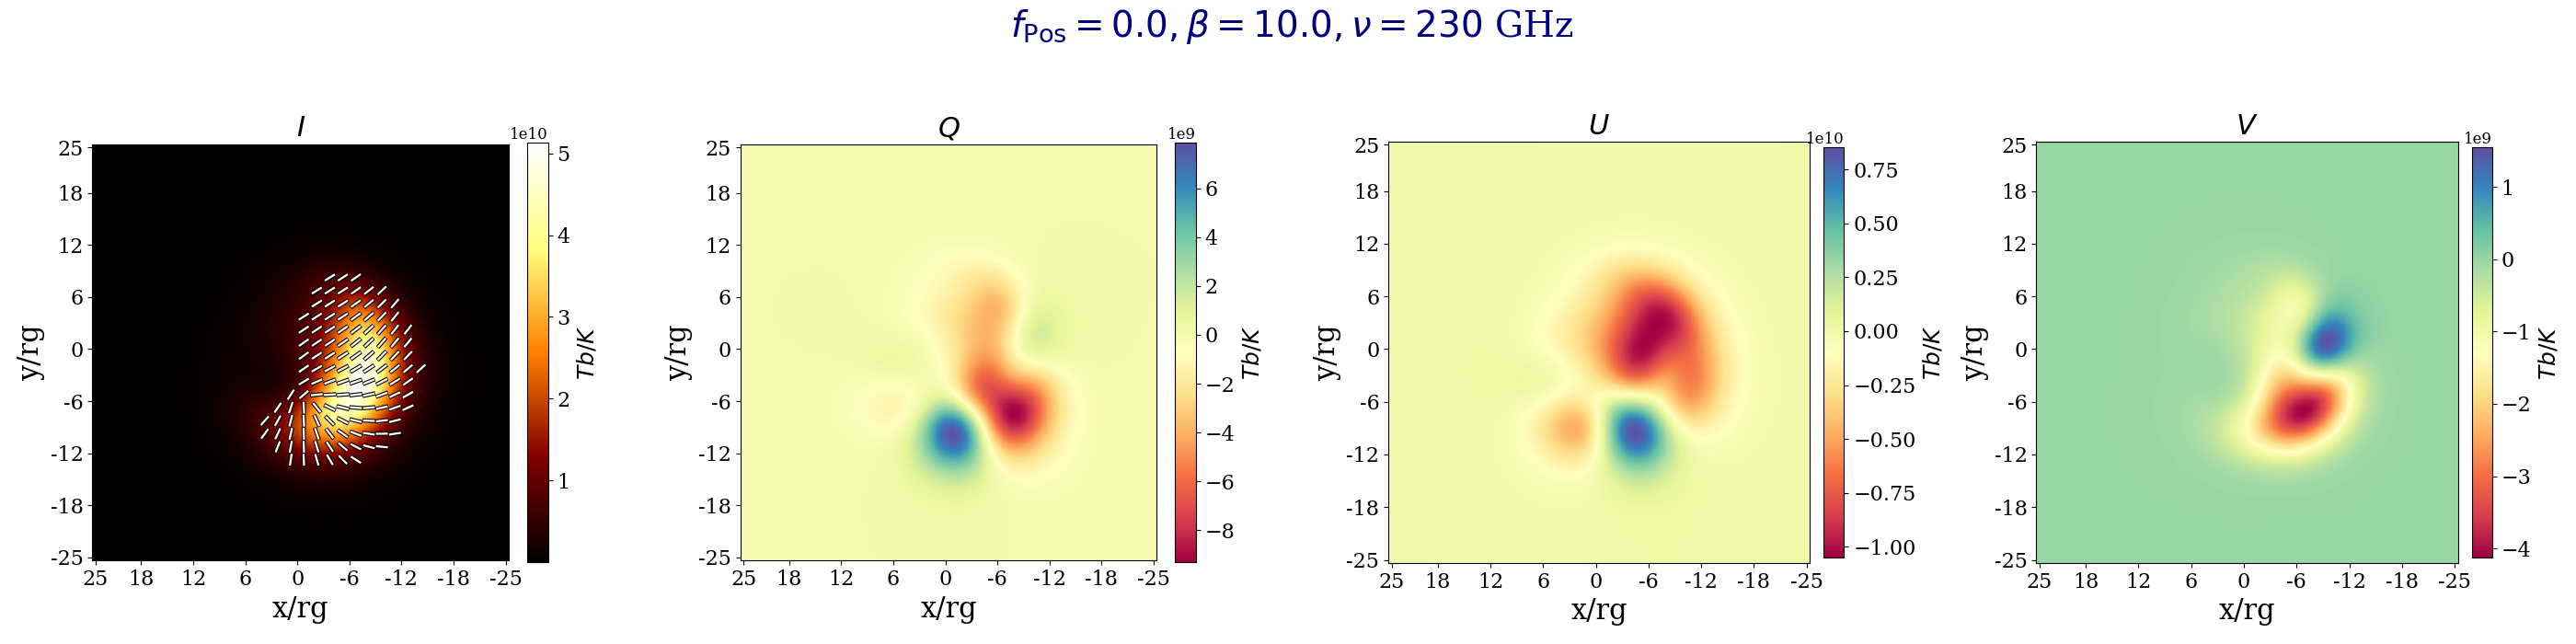
\includegraphics[width=.5\textwidth,height=27mm%,trim=0 380 0 200,clip
]{RIAFSgrAPlaneTscl1Pt5e11beta1Pt0e01fpos0Pt0fNTH1Pt0e-02copy}
  \caption{Polarization maps of Stokes parameters $I$, $Q$, $U$ and $V$ at 230 GHz for a \cite{Broderick2005} RIAF with $\beta=10$.}
  \label{fig:EmamiRIAF}
\end{figure}

\begin{figure}%[H]
%\begin{figure*}%[H]
%   \plotone{RIAFSgrAPlaneTscl1Pt5e11beta1Pt0e01fpos0Pt0fNTH1Pt0e-02copy.png}
  \includegraphics[width=.4\textwidth%width=.55\textwidth,height=25mm%,trim=0 380 0 200,clip
]{PositronModelEtAl2021RIAFPolSpectra%PolSpectscl1Pt5e11Beta1Pt0e1nth1Pt0em2fpos0Pt0
}
  \caption{Polarized SEDs for the Sgr A* RIAF model with  $\beta\in\{10^{-2},10^{0},10^{1}\}$, $f_\mathrm{pos}\in\{0.0,0.5,1.0\}$. The Top Panel shows the Stokes $I$ spectrum, while the Middle Panel shows the SED in linear polarization and the Bottom Panel shows the same for circular polarization.}
  \label{fig:EmamiRIAFSpectra}
%\end{figure*}
\end{figure}

%MOVED from Sect. 3.1 to Sect. 3.0
% \textcolor{red}{RJA: Include a summary of analytic/semi-analytic models and Sgr A* simulations in the Literature} Analytic disk $\alpha$-model for angular momentum transport \cite{Shakura1973}. Semi-analytic model motivated in \cite{Yuan2003} and expanded in \cite{Broderick2011}. GRMHD Simulation with hotspots reproducing Sgr A* flares \cite{Ripperda2020}.

\note{to be discussed: how much we would like to discuss polarization emission?}\textcolor{red}{RJA: We should mention the M87 Polarization Collaboration papers \cite{EHTCPaperVII}, including a comparison of whether Sgr A* is similar enough (e.g., MAD with vertical fields Faraday depolarized on much of the accretion flow) to have an azimuthally spiral EVPA pattern. Figures in  \citep{Emami2021} have similar morphology}.

\hyp{to-do :  adding historical RIAF fitting result to proto-EHT observations; how recent  GRMHD simulation and subsequent GRRT post-processing suggest other key parameters onto the Broderick 2005 RIAF model; jet componenet? cross referencing MCFE RIAF analysis product?} A proto-EHT array described in \cite{Doeleman2008} estimated the Sgr A* emitting region profile as a circular Gaussian with intrinsic size $37^{+16}_{-10}\ \mu$as.

% EHT flux vs. baseline observations constrain the emitting region intrinsic size to 37 microarcseconds for a circular Gaussian emission profile

More recent measurements of closure phases of a few degrees \cite{Fish2016} suggest an asymmetric ring-like profile, with major axis 56 microarcseconds

%==============================================================================
\subsection{Caveats and Limitations}

...

%==============================================================================
\subsection{Future Constraints}

\monika{this section should be moved to the end of the paper}
\ckc{Agree}

integrated polarization,

resolved polarization

fits to more sophisticated models such as RIAF analytic models,

closure phase variability


\section{Conclusions}
\label{sec:conclusions}

\begin{figure*}
  \centering
  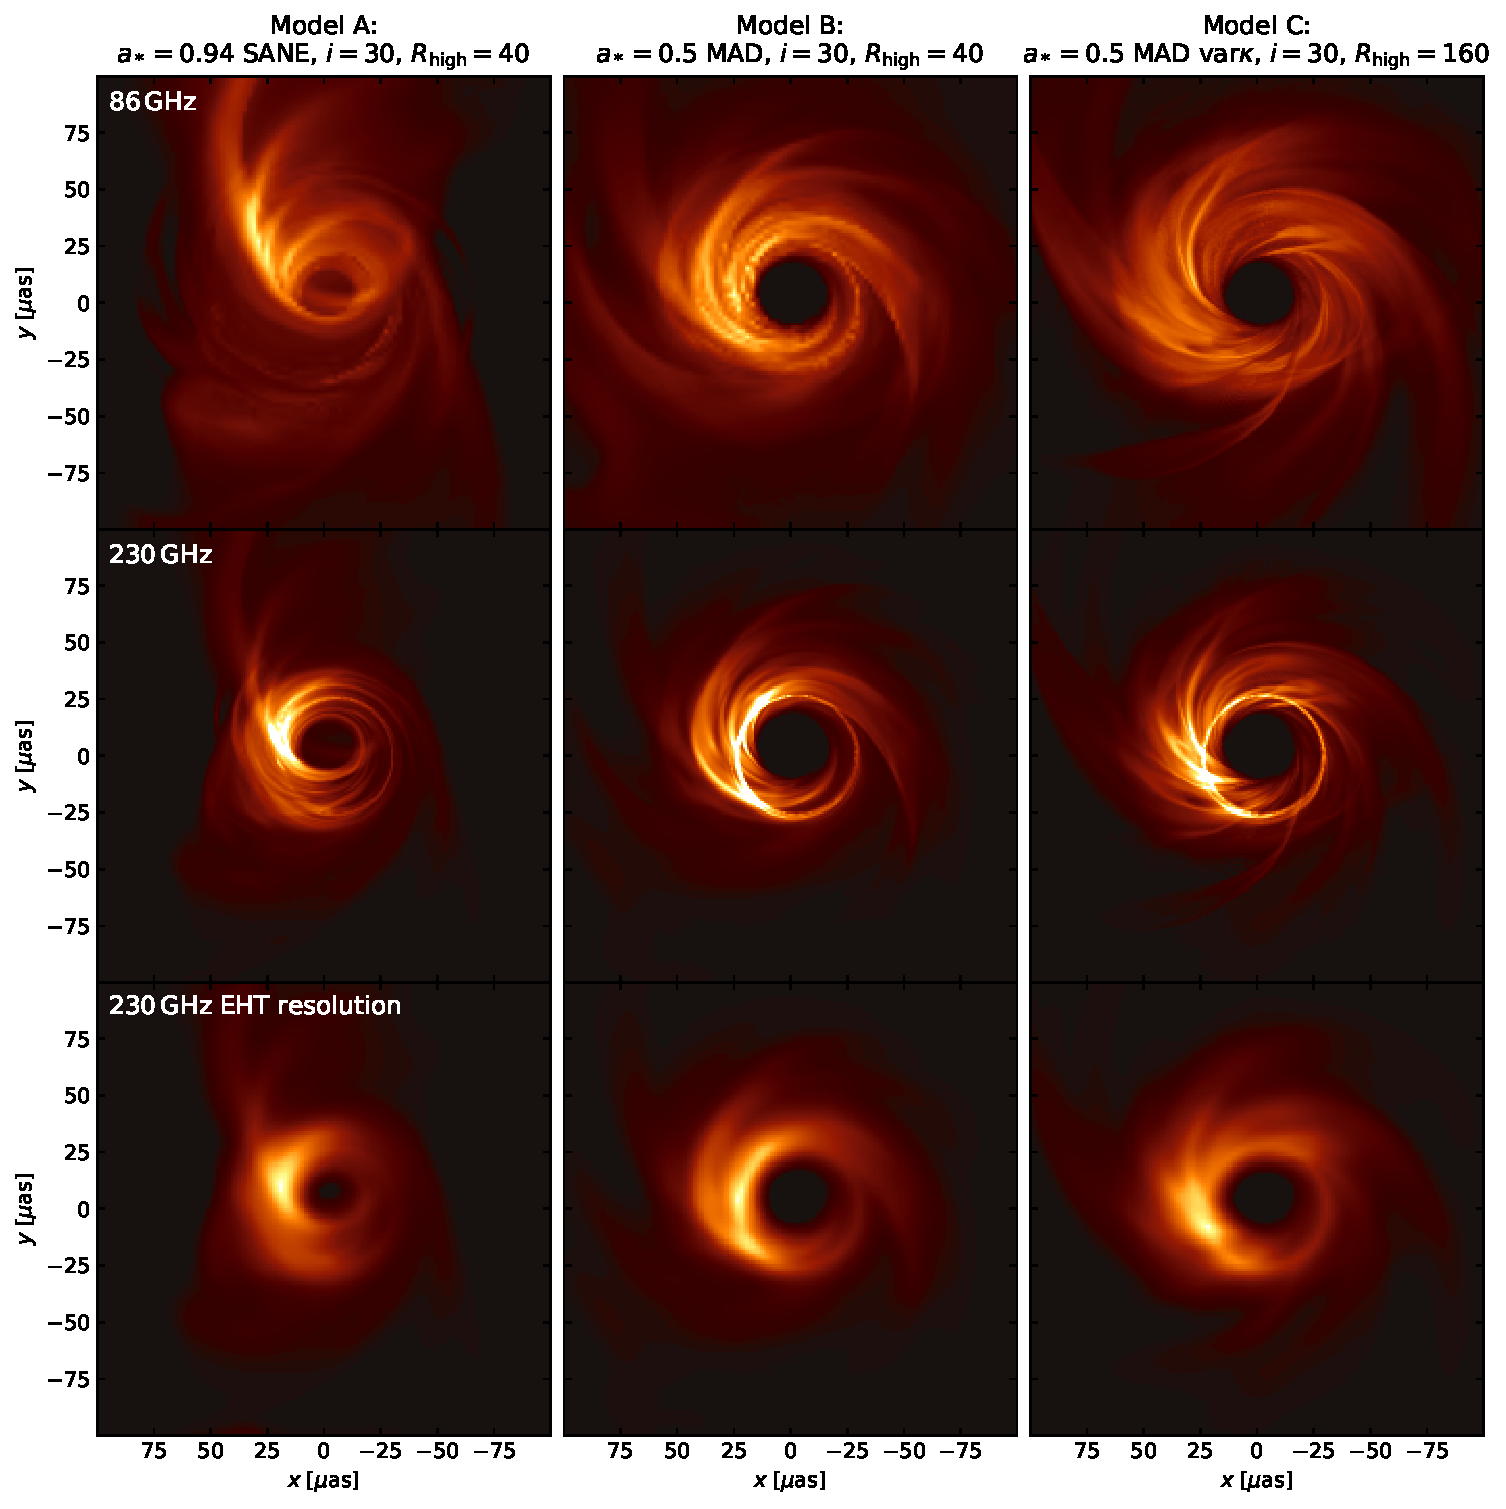
\includegraphics[width=\textwidth]{figures/bestbet_imgs.pdf}
  \caption{Best bet model that pass 10/11 constraints.
    The leftmost panel shows its 86\GHz ray traced image.
    The subsequent panels are the 230\GHz ray traced image,
    the 230\GHz image convolved with a 20\uas FWHM Gaussian for approximating the image at EHT resolution, and
    the actual reconstructed image from the EHT 2017 observation.
    Note that the position angle is not well constrained.
    So the rotation of the image here for matching the observed image is not statistically meaningful.}
  \label{fig:bestbet_imgs}
\end{figure*}

We have made a first comparison of the EHT 2017 \sgra data to a state-of-the-art library of ideal general relativistic magnetohydrodynamics (GRMHD) models.
The models assume that the mass and distance to \sgra are known and that the central object is a black hole described by the Kerr metric.
We use multiple simulation pipelines and find that for a given set of initial and boundary conditions, independent simulations are remarkably consistent (see Appendix~\ref{app:numerical}).

The model parameters are: whether the horizon magnetic field is strong or weak (MAD or SANE, respectively); the black hole spin $\abh$; and the inclination angle $i$ between the line of sight and the black hole spin vector.
The electron distribution function (eDF) also has one or more parameters.
In our ``standard'' model set, run with three independent codes, the eDF is determined using the so-called $\Rh$ prescription (see Section \ref{sec:models}).
We have also considered non-standard models with alternate eDF prescriptions and alternate initial conditions.

We have selected and applied 11 heterogeneous observational constraints.
Six derive directly from EHT VLBI data, two derive from 86\GHz VLBI observations with the GMVA, one from variability of the 230\GHz lightcurve, and one each from the 2.2\um flux density and the X-ray luminosity.

Five structural constraints derive from EHT VLBI data.
While these constraints are not independent, which makes their interpretation as likelihood difficult, the multiple constraints make our analyses more robust.
When combined these constraints reject about 75\% of our standard models.
The EHT cut favors $\abh \ge 0$ and avoids edge-on ($i = 90\degree$) models and models with equal ion and electron temperatures ($\Rh = 1$).
We are {\em not} able to constrain the source position angle due to sparse baseline coverage.
The 2017 EHT observations are, nevertheless, quite constraining; new EHT observations with more baselines will be even more constraining.

Four constraints derive from non-EHT data that are contemporaneous or near-contemporaneous.
Combined, the non-EHT constraints reject 88\% of standard models.
The non-EHT cut favors strongly magnetized (MAD) models, eliminates all models with equal ion and electron temperatures, and eliminates most models at $i > 50\degree$.
These results highlight the value of continued multiwavelength monitoring of \sgra.

\sgra is variable.
We have used two tests to compare the variability of models and data.
One characterizes variability in the 230\GHz lightcurve (including simultaneous ALMA data) and the other structural characterizes variability expressed through fluctuations in the visibility amplitudes.
The lightcurve variability is the tightest of all 11 constraints: it rejects 77\% of our standard models.
We find that strongly magnetized (MAD) models are more variable than weakly magnetized (SANE) models and, grouped together, both SANE and MAD models are more variable than the data.
The structural variability measures the slope and amplitude of the power spectrum of the VA variability.
Remarkably, we find that the power spectrum slope is consistent for all models, while the power spectrum amplitude is inconsistent for 34\% of standard models.

The failure of most standard models to match the lightcurve variability is interesting.
It may signal the presence of extended, slowly varying structure that is resolved out by EHT, or it may signal that future models need to incorporate collisionless effects (potentially modeled as viscosity and conductivity) or a more sophisticated treatment of electron thermodynamics including cooling.
If each of these effects reduces $\mi{3}$ by about $10\%$ then many of the MAD models would be consistent with the data.

None of the standard models survive the full gauntlet of 11 constraints.
If we set aside variability, however, there is a cluster of 3 models that pass the remaining 10 constraints in both the Illinois and Frankfurt standard models (a few more survive in one model set but not the other).
These ``best-bet'' models are are strongly magnetized (MAD) and have $\Rh = 160$, positive spin, and low inclination ($\abh, i = 0.5, 30; 0.94, 10; 0.94; 30$).
Images of the best-bet models are shown in Figure \ref{fig:bestbet_imgs}, along with the observed image.


Our cluster of best-bet models has accretion rate $\dot{M} = 5.2$--$9.5 \times 10^{-9}\msun\yr^{-1}$.
These accretion rates are consistent with earlier estimates and overlap with accretion rates in wind-fed models, $\sim 10^{-8} \msun\yr^{-1}$ \citep{2020ApJ...896L...6R}.
The $\abh = 0.5$ MAD with $i=30$ model is presented in Figure~\ref{fig:bestbet_imgs}, together with a smoothed image that matches the EHT resolution and one of the reconstruction from the 2017 EHT observation.

We produced synthetic SEDs, and therefore bolometric luminosities $L_\mathrm{bol}$, for all standard models.
Typically $L_\mathrm{bol}$ is dominated by a synchrotron bump in the submm and for the best-bet models is $6.8$--$9.8\times10^{35}\ergps$; the corresponding radiative efficiency $L_\mathrm{bol}/(\dot{M} c^2)$ is $1.3$--$3.0\times 10^{-3}$.
The maximum radiative efficiency over the entire standard model set is 0.08 (for a MAD, $\abh = 0.94$, $\Rh = 1$ model), which is necessary but not sufficient to justify our neglect of radiative cooling in the GRMHD evolution.

All our models produce bipolar outflows, and for each we measured the outflow power $P_\mathrm{out}$, defined in Section~\ref{sec:discussions}.
Consistent with earlier work we find that outflow power is higher for strongly magnetized (MAD) models than for comparable weakly magnetized (SANE) models, and increases by more than an order of magnitude from $\abh = 0$ to $|\abh| = 0.94$.
For the best-bet models $P_\mathrm{out} = 1.3$--$4.8 \times 10^{38}\ergps$, corresponding to an outflow efficiency $P_\mathrm{out} /(\dot{M} c^2)$ of 0.25--1.6.
Such large  outflow efficiency is only possible if energy is extracted from a spinning black hole via the mechanism proposed by  \cite{1977MNRAS.179..433B}.
It is an open question how these powerful outflows might interact with incoming gas in a self-consistent accretion model that follows plasma over a larger range in radius than our standard models.
It is also an open question whether the outflow power could be detected in the dense but crowded galactic center environment.
Notice that this outflow luminosity is comparable to the spindown luminosity of the Crab pulsar.

Our standard models assume a particular parameterization for the electron distribution function (the $\Rh$ prescription), use a common initial setup (a magnetized torus), and assume the black hole spin vector and torus angular momentum are aligned or anti-aligned.
To partially control for the errors introduced by these assumptions we have explored a set of nonstandard models.
The nonstandard models include several eDF prescriptions, a wind-fed model that tracks accretion from stellar winds down to the scale of the horizon, and tilted disk models in which the black hole spin and torus angular momentum are misaligned.

Our nonthermal models do not differ substantially from their thermal counterparts.
For the limited set of nonthermal eDF prescriptions we consider here the 230\GHz image structure differs very little.
The 230\GHz variability is not detectably different than corresponding thermal models.\footnote{The nonthermal models are imaged over $5\times 10^3\tg$, so constraints on $\mi{3}$ are weaker than for the standard models, which are imaged for 3 times as long.}
The 86\GHz size and flux density, which are the most restrictive non-EHT constraints, are not detectably affected by the addition of nonthermal electrons for most nonthermal models (except $\kappa = 5$ models).
Nonthermal electrons consistently increase the 2.2\um flux density over similar thermal models, however.
Accelerating even a small fraction of the electron population into a nonthermal tail risks overproducing 2.2\um emission.
The 2.2\um (and submm through mid-IR) flux density therefore provides the strongest eDF constraints.
Future EHT analyses would benefit from incorporating submm constraints \citep[e.g.,][]{2019ApJ...881L...2B} and, because model submm SEDs are highly variable, the submm and 2.2\um data should be near-simultaneous as possible.

The stellar wind-fed models of \cite{2020ApJ...896L...6R} feature the best-motivated treatment of boundary and initial conditions for \sgra models.
They differ from our torus-initialized standard models in that they follow plasma from its ejection from stars on known orbits down to the event horizon.
We have imaged these models using an $\Rh$ prescription for the electron temperature, with $\Rh$ adjusted in the otherwise parameter-free models to produce the correct time-averaged 230 GHz flux density.
The two models considered here, both with $\abh = 0$, fail the 86\GHz flux, \mring width, and $\mi{3}$ constraints.
This does {\em not} imply that wind fed models are ruled out; they clearly merit further investigation with longer integrations over a broader range of eDFs and $\abh$.

In general, black hole accretion flows can be tilted in the sense that the orbital angular momentum of the disk and the spin angular momentum of the hole are misaligned.
Tilted disks have not been included in EHT analyses because \emph{i}) it is conceivable that accretion flows align either by consistently oriented long term accretion or by some analog of the Bardeen-Petterson effect \citep{1975ApJ...195L..65B} and \emph{ii}) the tilted disk parameter space is larger than the aligned disk parameter space by two dimensions: the tilt angle and the longitude of the observer.
We considered models with tilt $30\degree$ and $60\degree$, observed at a single longitude.
The integrations were too short ($3000\tg$) to provide strong constraints on tilt, but we find that the \mring width test is particularly sensitive to tilt and rejects a progressively larger fraction of the models as tilt increases at the single observing longitude studied here.
Tilted models clearly merit further investigation.

Our standard models and variable $\kappa$ nonthermal models have been run with independent GRMHD codes and imaged with independent radiative transfer codes.
The outcomes are largely consistent (see Appendix~\ref{app:numerical} for details).
The code comparisons were valuable and helped us identify multiple issues in the independent simulation sets.
The consistency between codes is remarkable given the complexity of the modeling process and the scope for error.
Tracking down the remaining discrepancies (for example, in the 2.2\um flux density) and developing a quantitative error budget is an essential but difficult task for the future.

This first comparison of the EHT 2017 \sgra data to state-of-the-art GRMHD models shows remarkable successes and highlights interesting problems, including the origin of variability.
The observational constraints considered here put pressure on the theoretical models and have shown that the models are not trivially adjustable to pass all tests.
This work signals the arrival of a new era of precision black hole astrophysics in which close interaction of theory and experiment has the potential to unveil the inner workings of the galactic center.


%------------------------------------------------------------------------------
\facility{EHT} \software{\difmap, \dmc, \ehtim, \foci, \hallmark, \mockservation, \smili, \themis}

%------------------------------------------------------------------------------
\appendix

%\section{Model Details}\label{app:models}

\begin{figure}
  \centering
  \note{altex: averaged image grid}
  \caption{Averaged images as functions of parameters}
  \label{fig:imgs}
\end{figure}

\begin{figure}
  \centering
  \note{altex: averaged SEDs}
  \caption{Averaged SEDs as functions of parameters}
  \label{fig:seds}
\end{figure}

\begin{figure*}
  \centering
  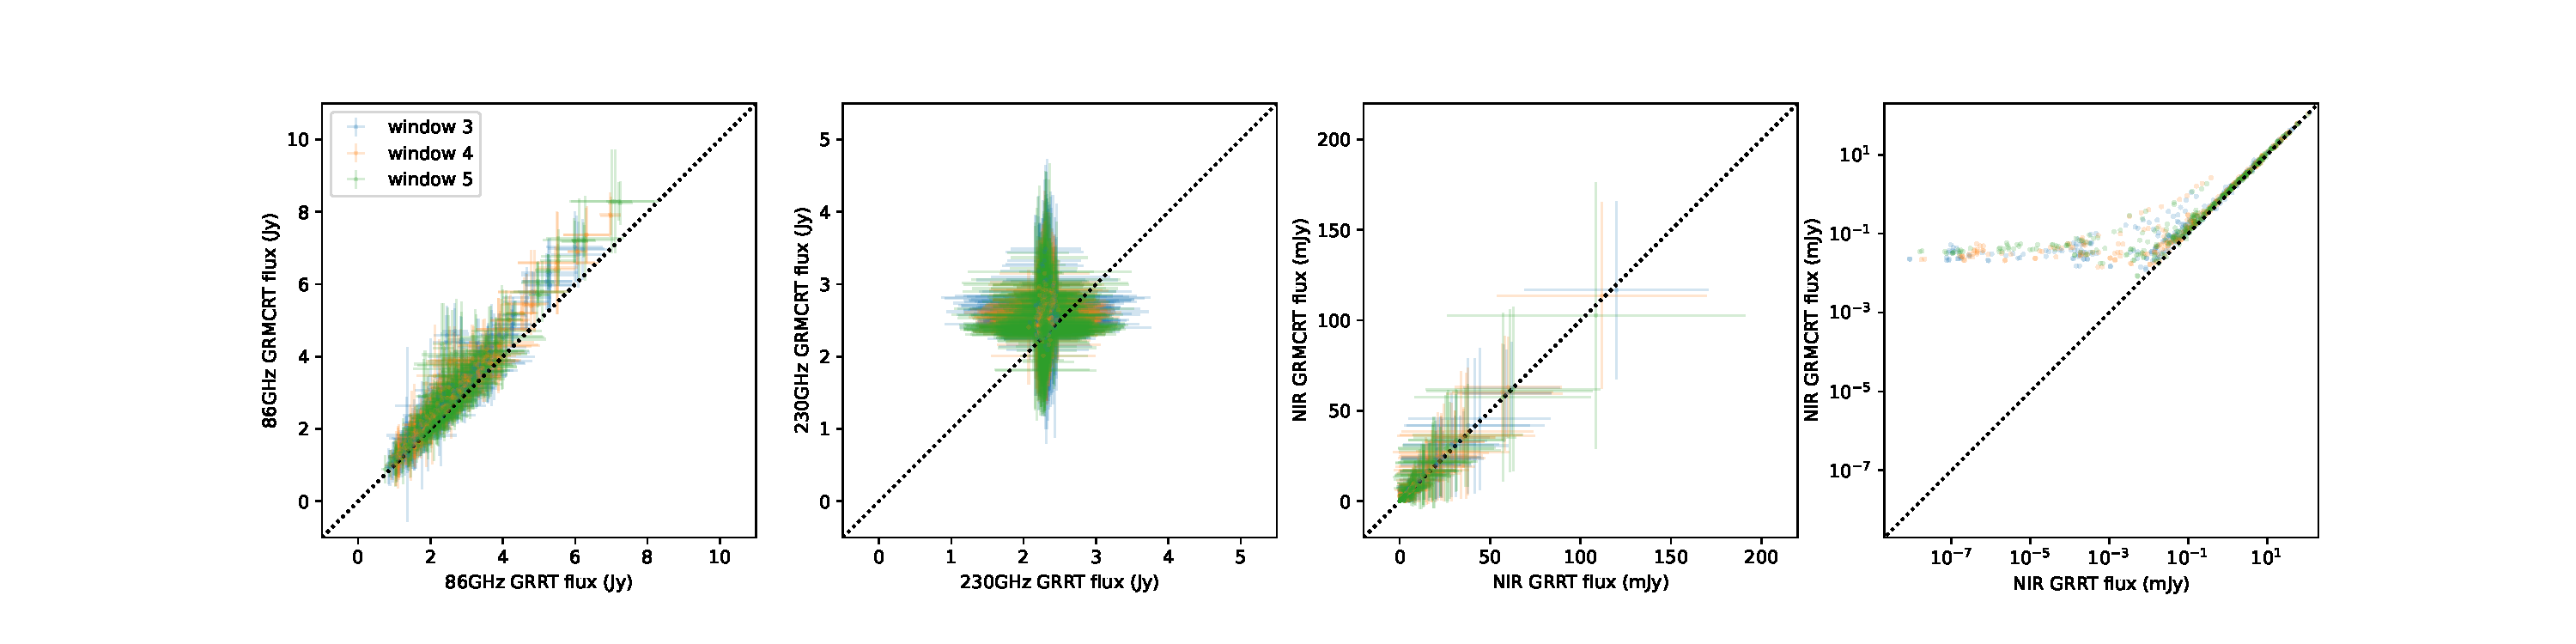
\includegraphics[width=\textwidth]{figures/GRRT_vs_MCRT.pdf}
  \caption{Compare fluxes computed from GRRT and MCRT.}
  \label{fig:GRRT_vs_MCRT}
\end{figure*}

%\clearpage

\section{Pass/Fail Plots and Tables}\label{app:tables}

%\pagebreak
%\movetabledown=3cm
%\movetableright=-7cm

In this appendix we present the full results of the constraint application in both graphical and tabular form.

First the EHT-based constraints on the Illinois thermal model set.

\begin{figure*}
  \centering
  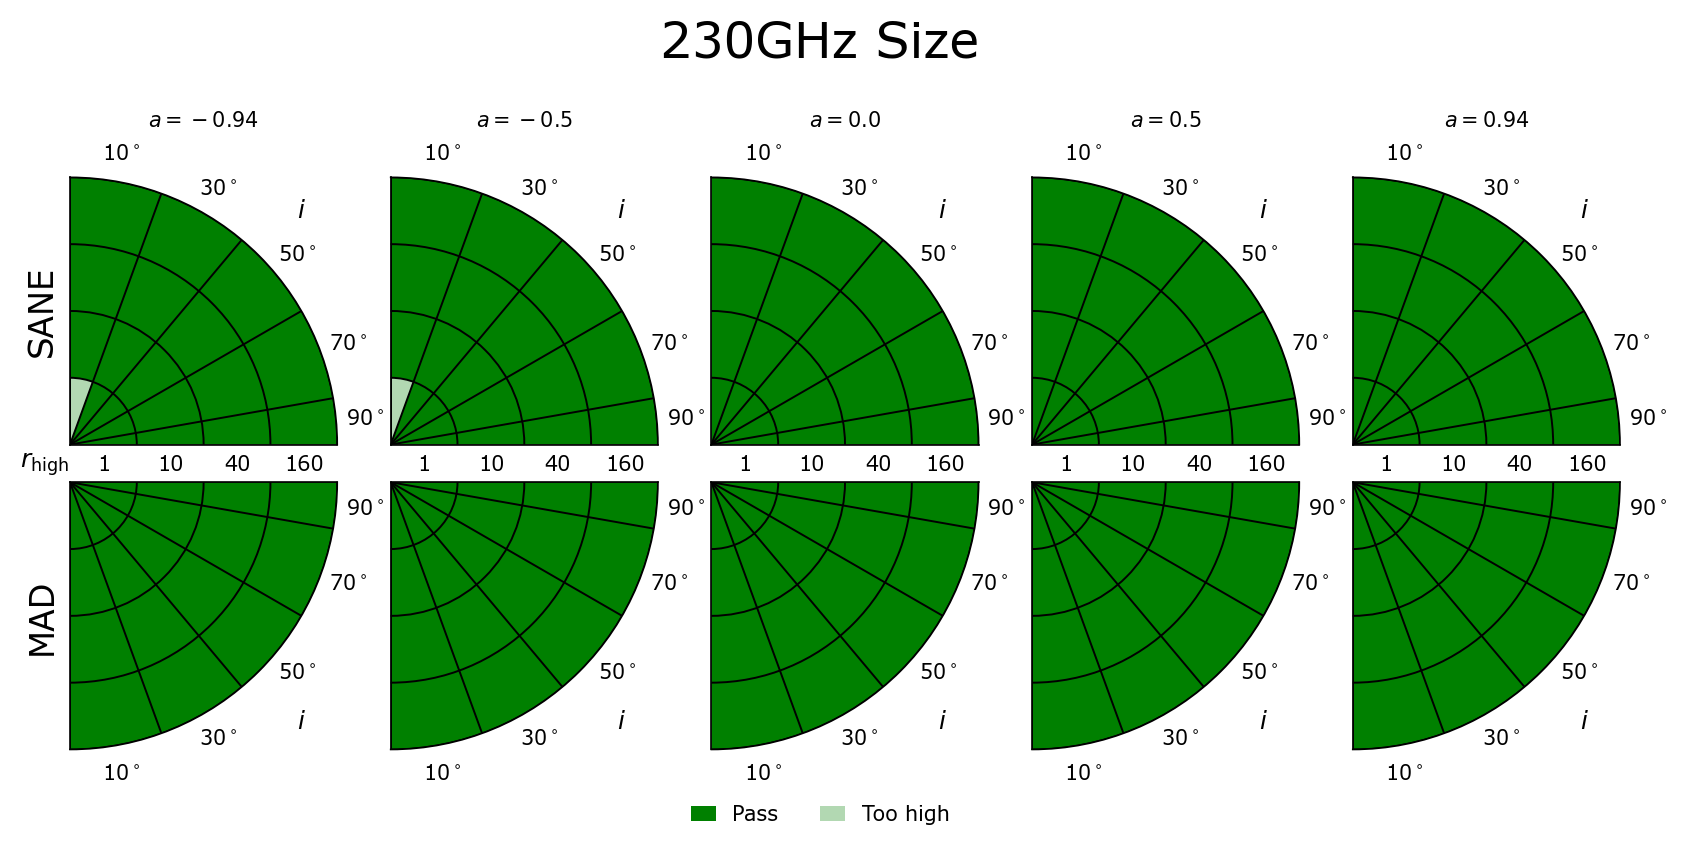
\includegraphics[width=0.8\textwidth]{./figures/230GHz_size_Constraints.png}
  \caption{2nd Moment Constraint}
  \label{fig:230GHz_size_pizza}
\end{figure*}
\begin{figure*}
  \centering
  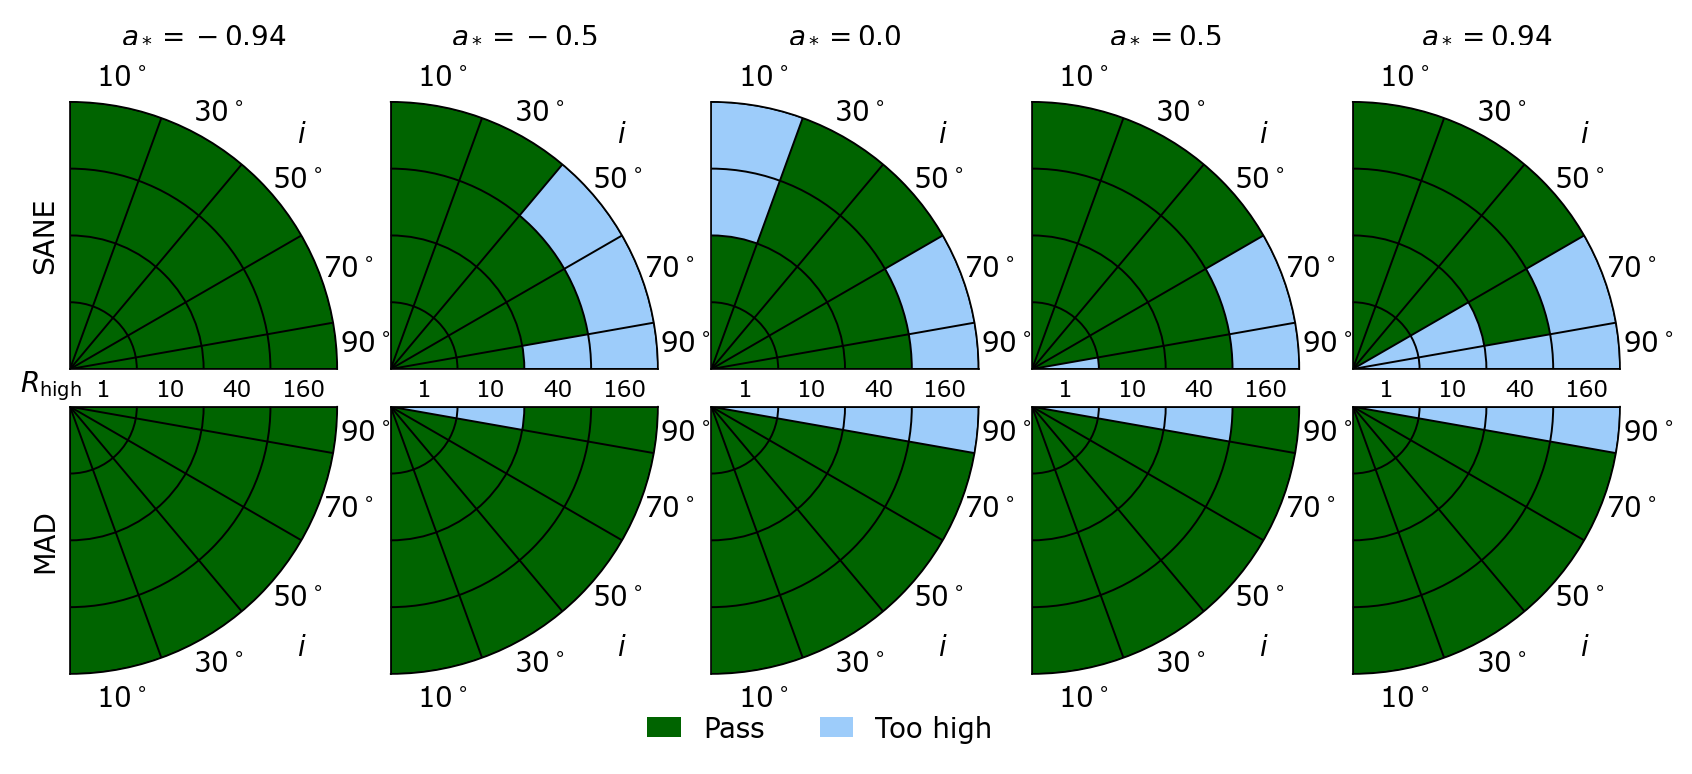
\includegraphics[width=0.8\textwidth]{./figures/Null_loc_Constraints.png}
  \caption{Null Location Constraint}
  \label{fig:null_pizza}
\end{figure*}
\begin{figure*}
  \centering
  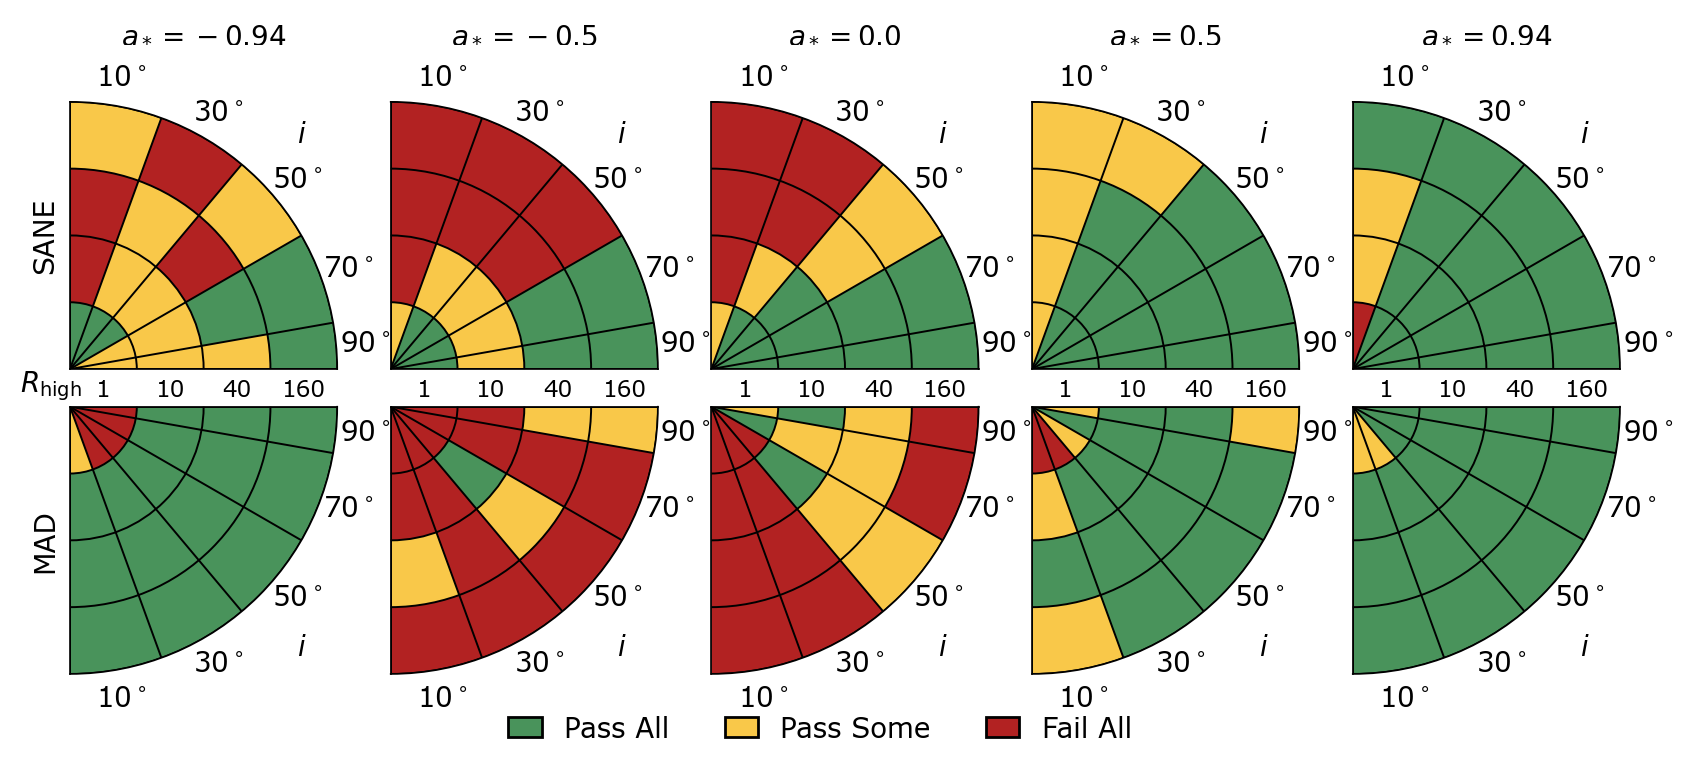
\includegraphics[width=0.8\textwidth]{./figures/Mring_d_Constraints.png}
  \caption{M-ring Diameter Constraints}
  \label{fig:mring_diam_pizza}
\end{figure*}
\begin{figure*}
  \centering
  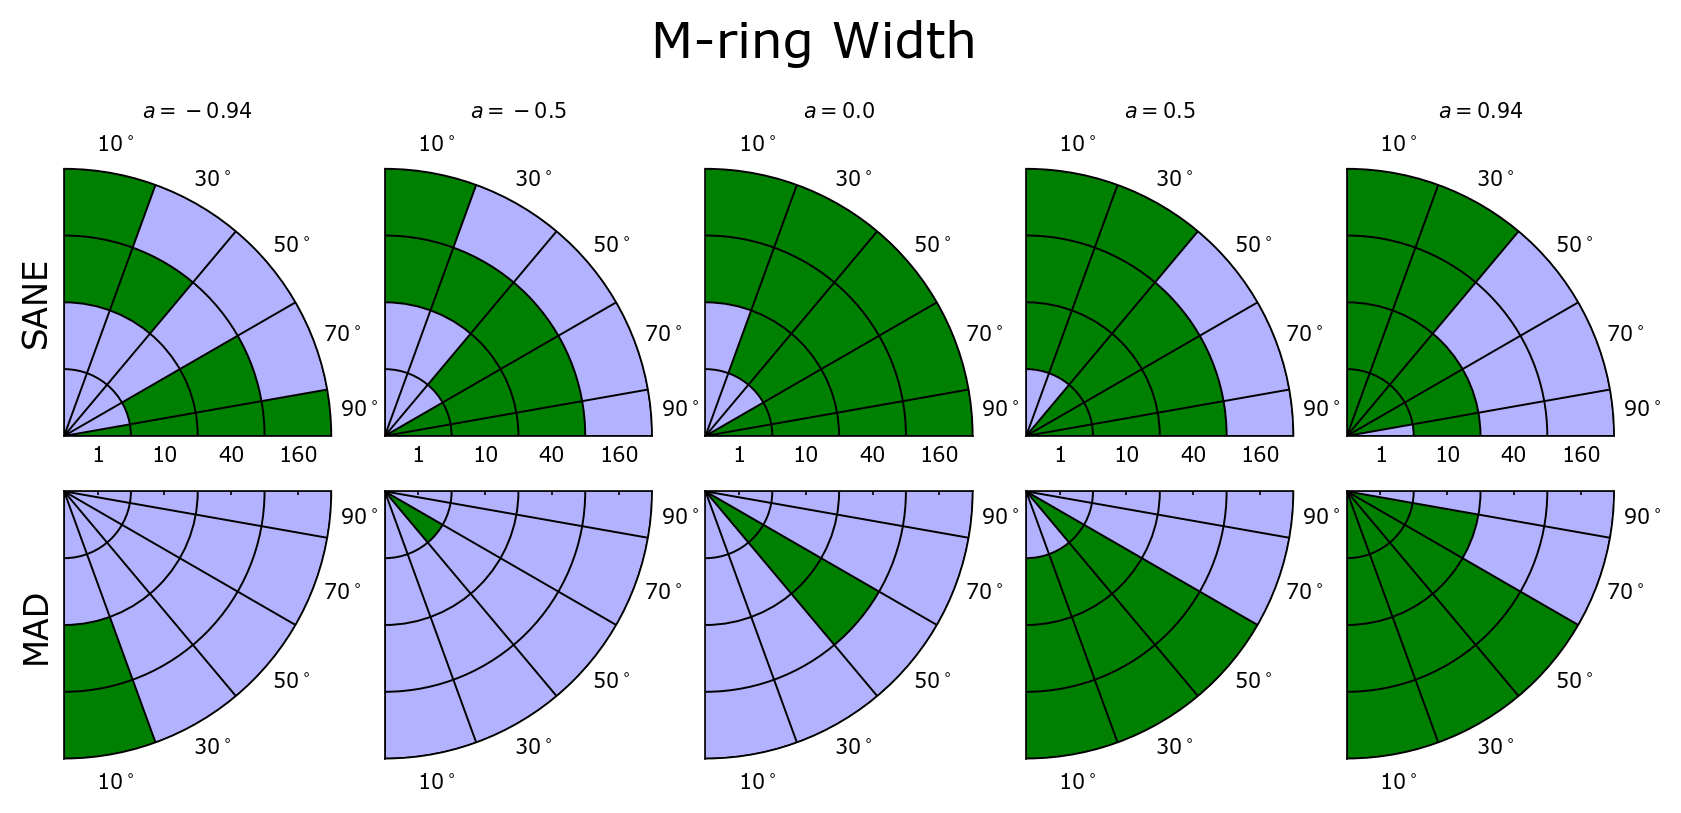
\includegraphics[width=0.8\textwidth]{./figures/Mring_w_Constraints.png}
  \caption{M-ring Width Constraints}
  \label{fig:mring_width_pizza}
\end{figure*}
\begin{figure*}
  \centering
  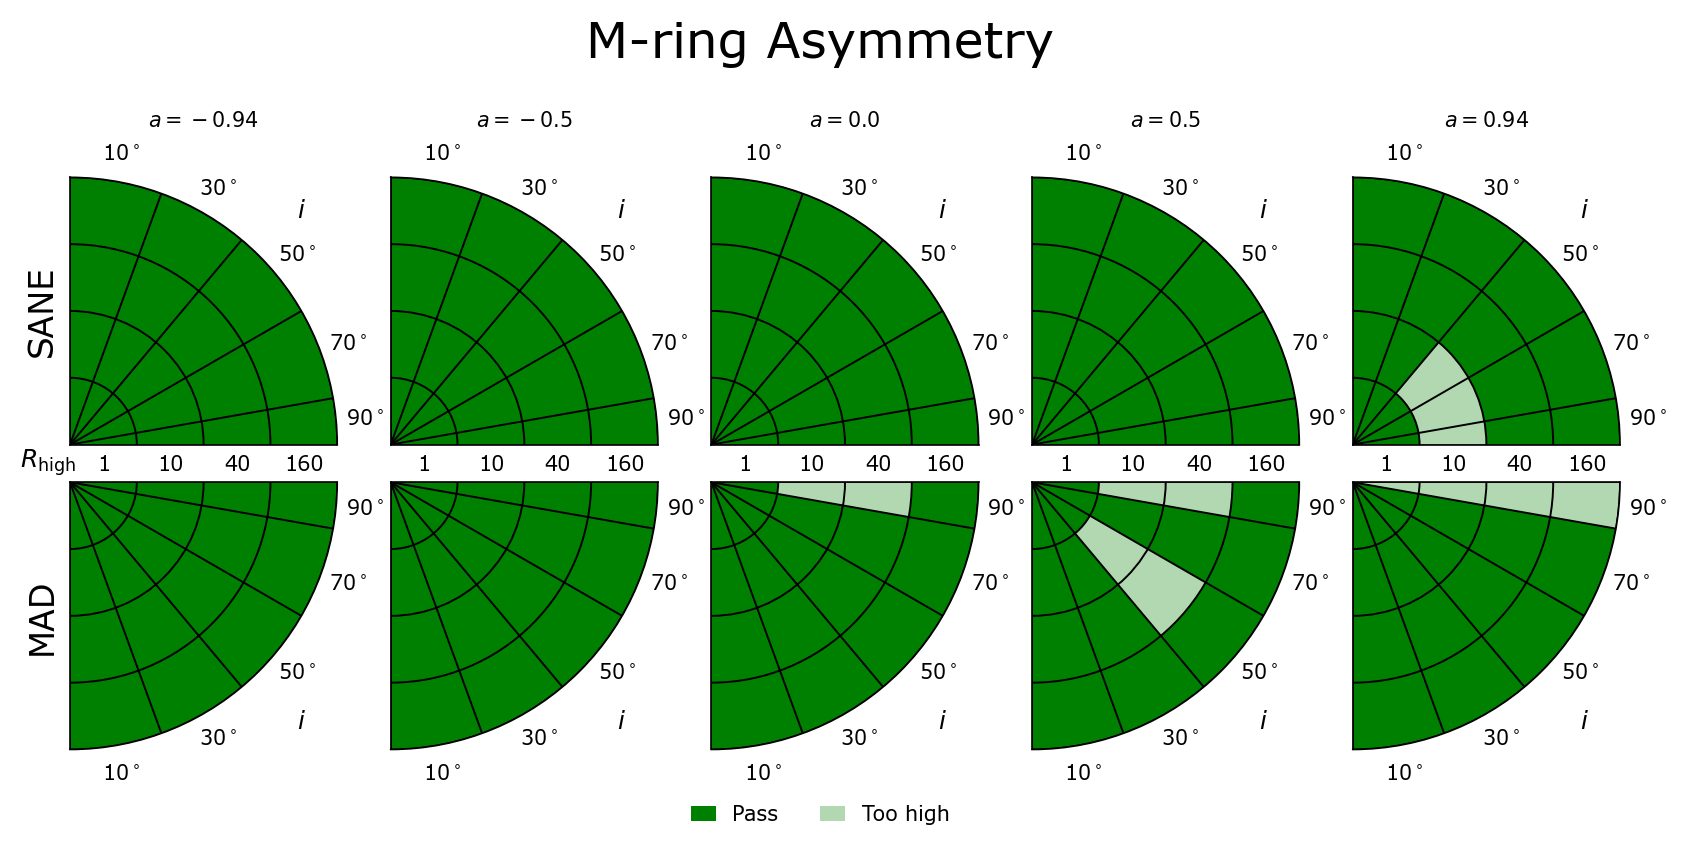
\includegraphics[width=0.8\textwidth]{./figures/Mring_f1_Constraints.png}
  \caption{M-ring Asymmetry Constraints}
  \label{fig:mring_asymm_pizza}
\end{figure*}
\begin{figure*}
  \centering
  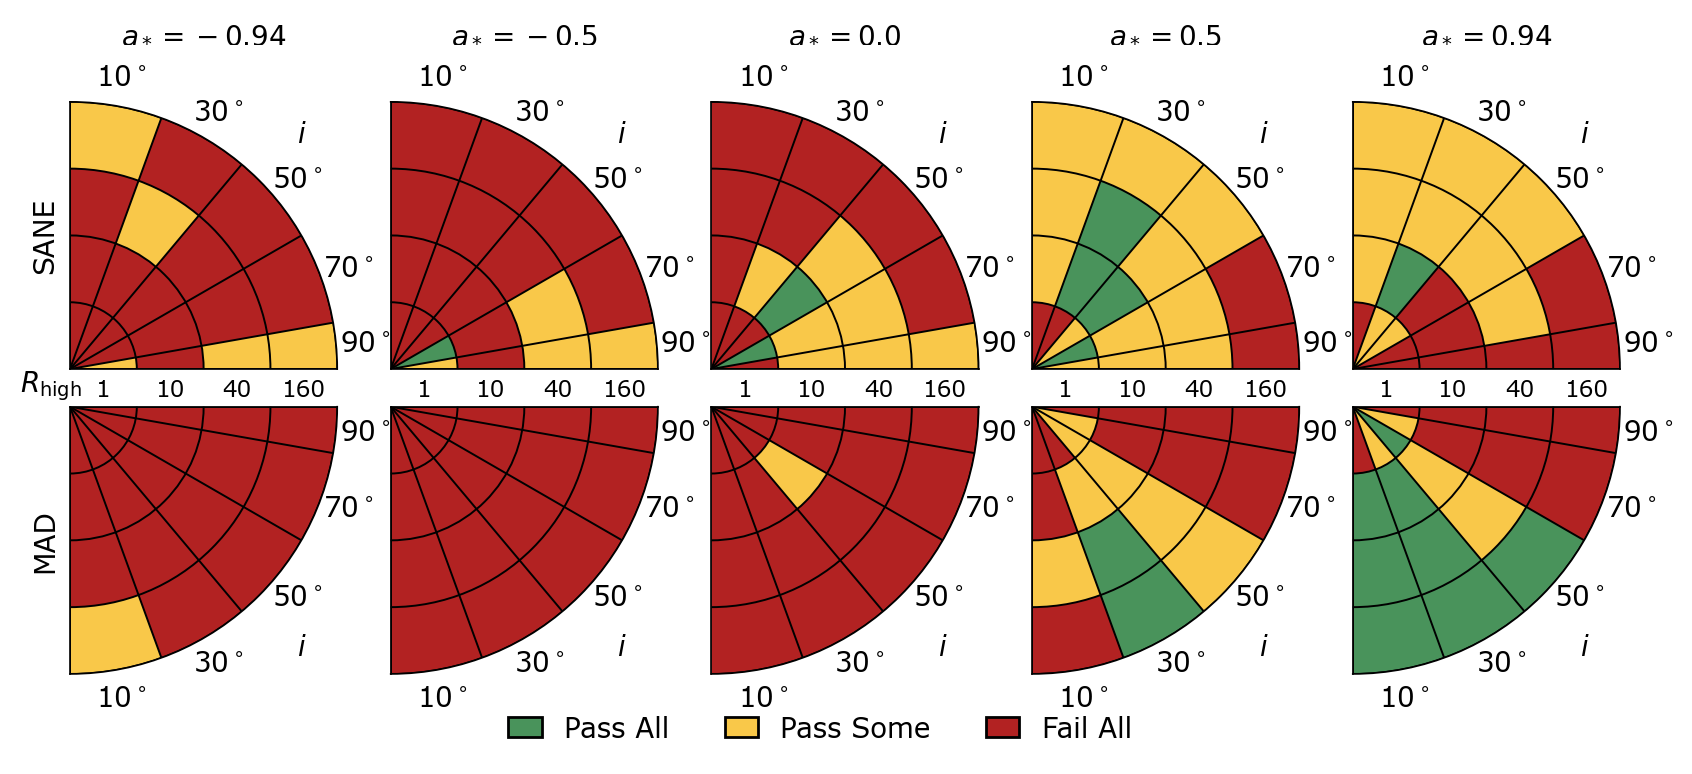
\includegraphics[width=0.8\textwidth]{./figures/Interferometric_Constraints.png}
  \caption{Combined EHT Constraints}
  \label{fig:eht_comb_pizza}
\end{figure*}

Then the non-EHT constraints.

\begin{figure*}
  \centering
  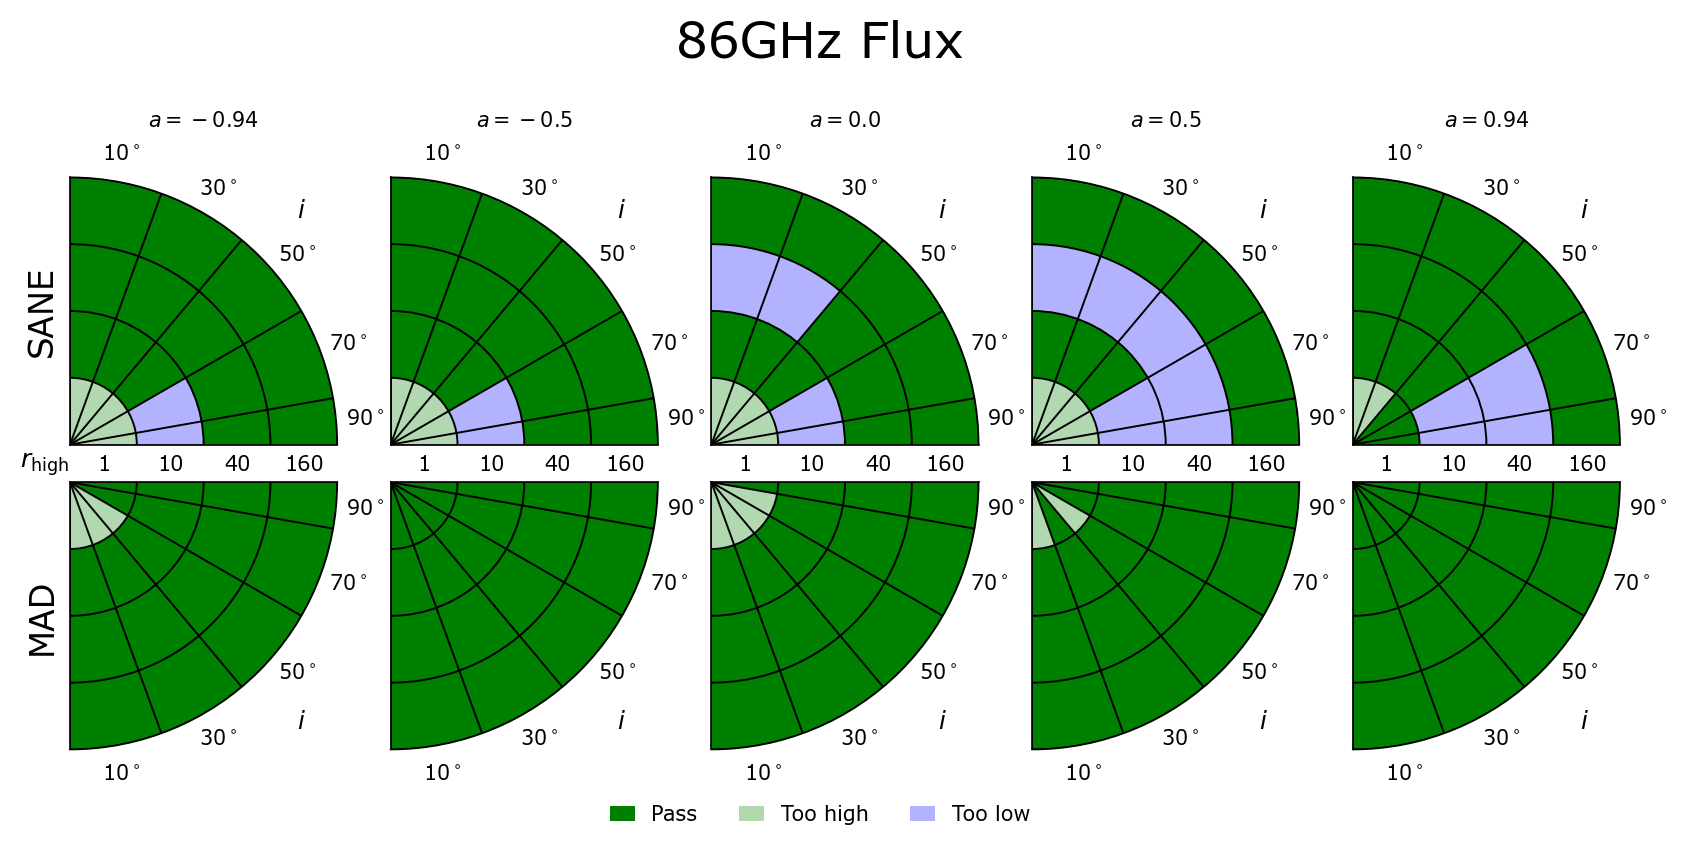
\includegraphics[width=0.8\textwidth]{./figures/86GHz_flux_Constraints.png}
  \caption{86GHz Flux Constraints}
  \label{fig:86GHz_flux_pizza}
\end{figure*}
\begin{figure*}
  \centering
  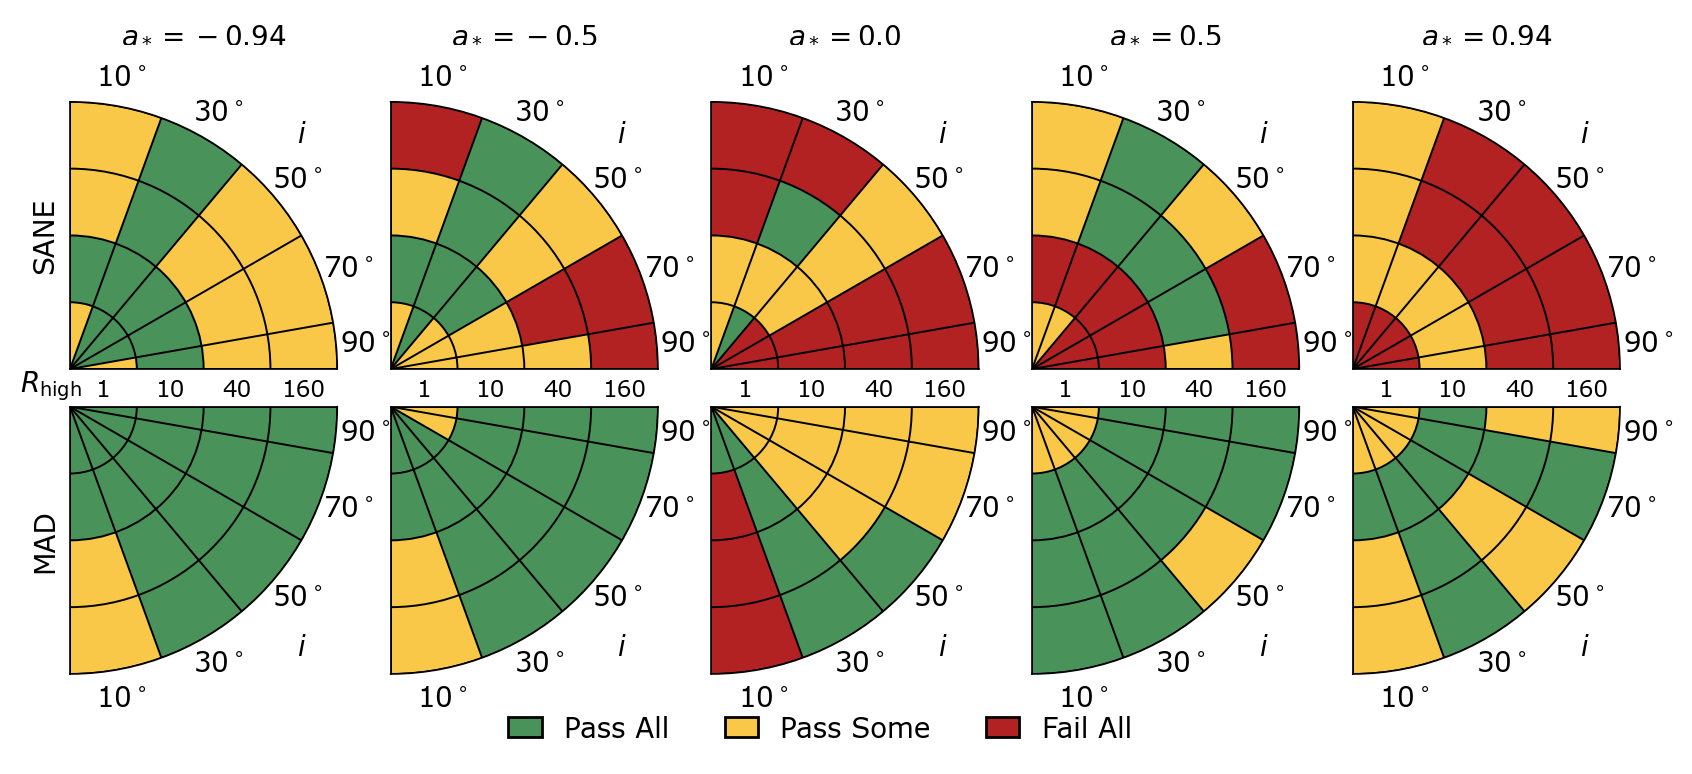
\includegraphics[width=0.8\textwidth]{./figures/86GHz_size_Constraints.png}
  \caption{86GHz Size Constraints}
  \label{fig:86GHz_size_pizza}
\end{figure*}
\begin{figure*}
  \centering
  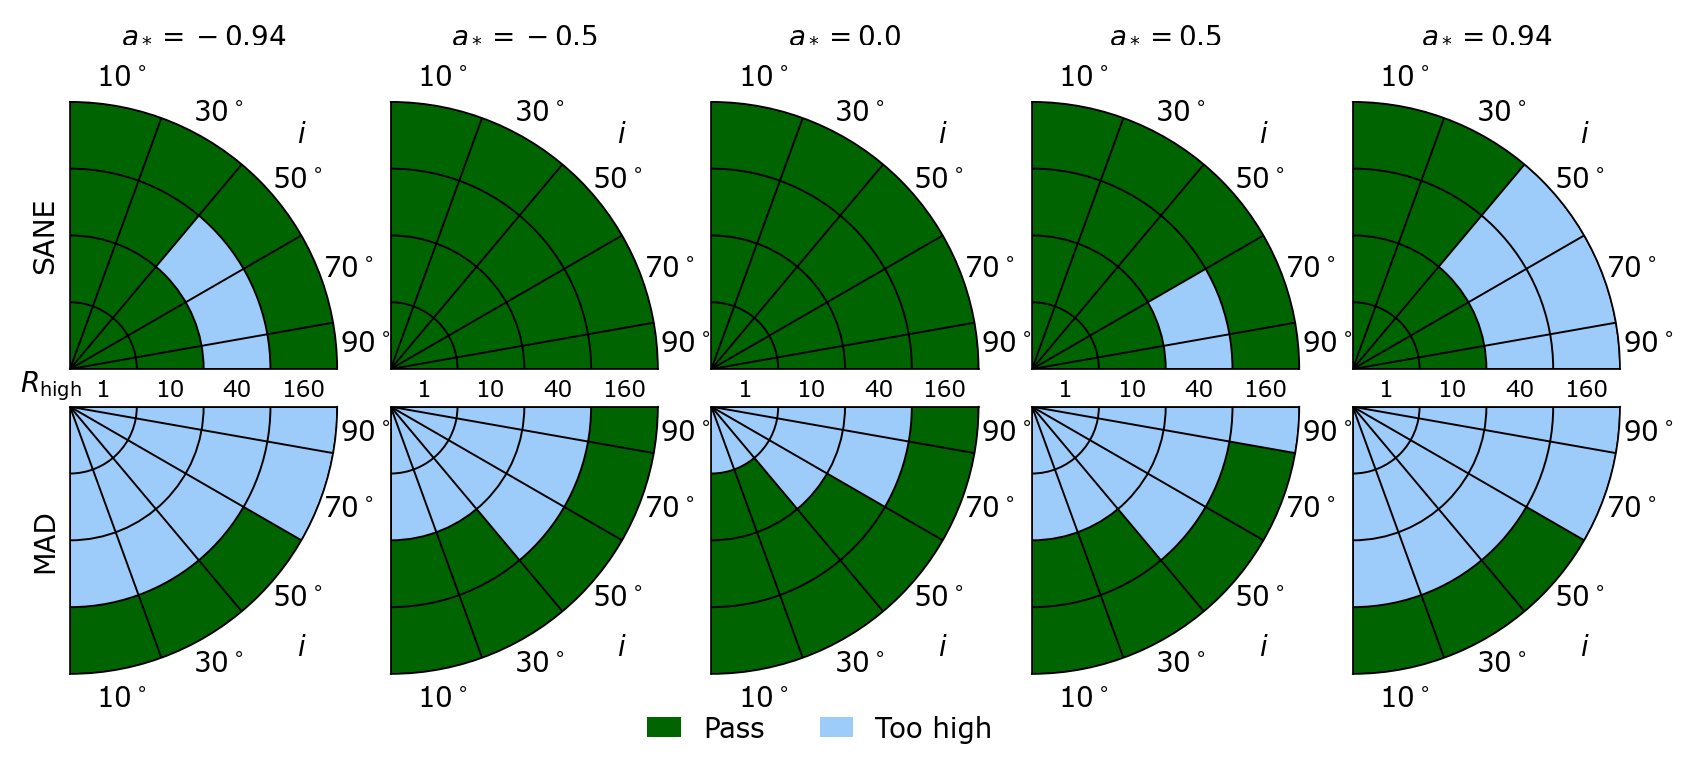
\includegraphics[width=0.8\textwidth]{./figures/2um_flux_Constraints.png}
  \caption{2$\mu$m Flux Constraints}
  \label{fig:2um_flux_pizza}
\end{figure*}
\begin{figure*}
  \centering
  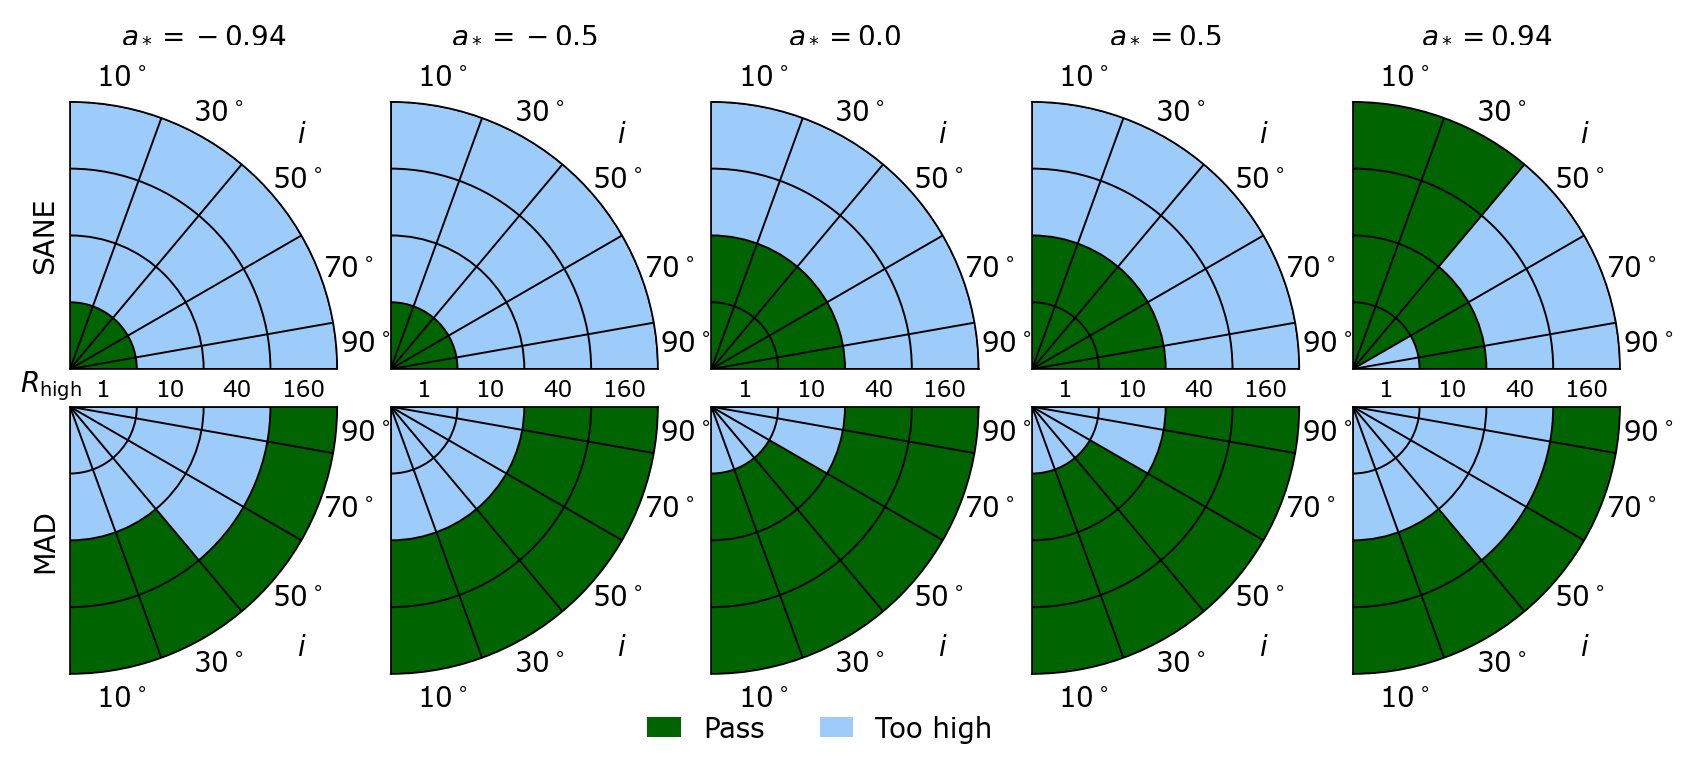
\includegraphics[width=0.8\textwidth]{./figures/Xray_flux_Constraints.png}
  \caption{X-Ray Luminosity Constraints}
  \label{fig:xray_pizza}
\end{figure*}
\begin{figure*}
  \centering
  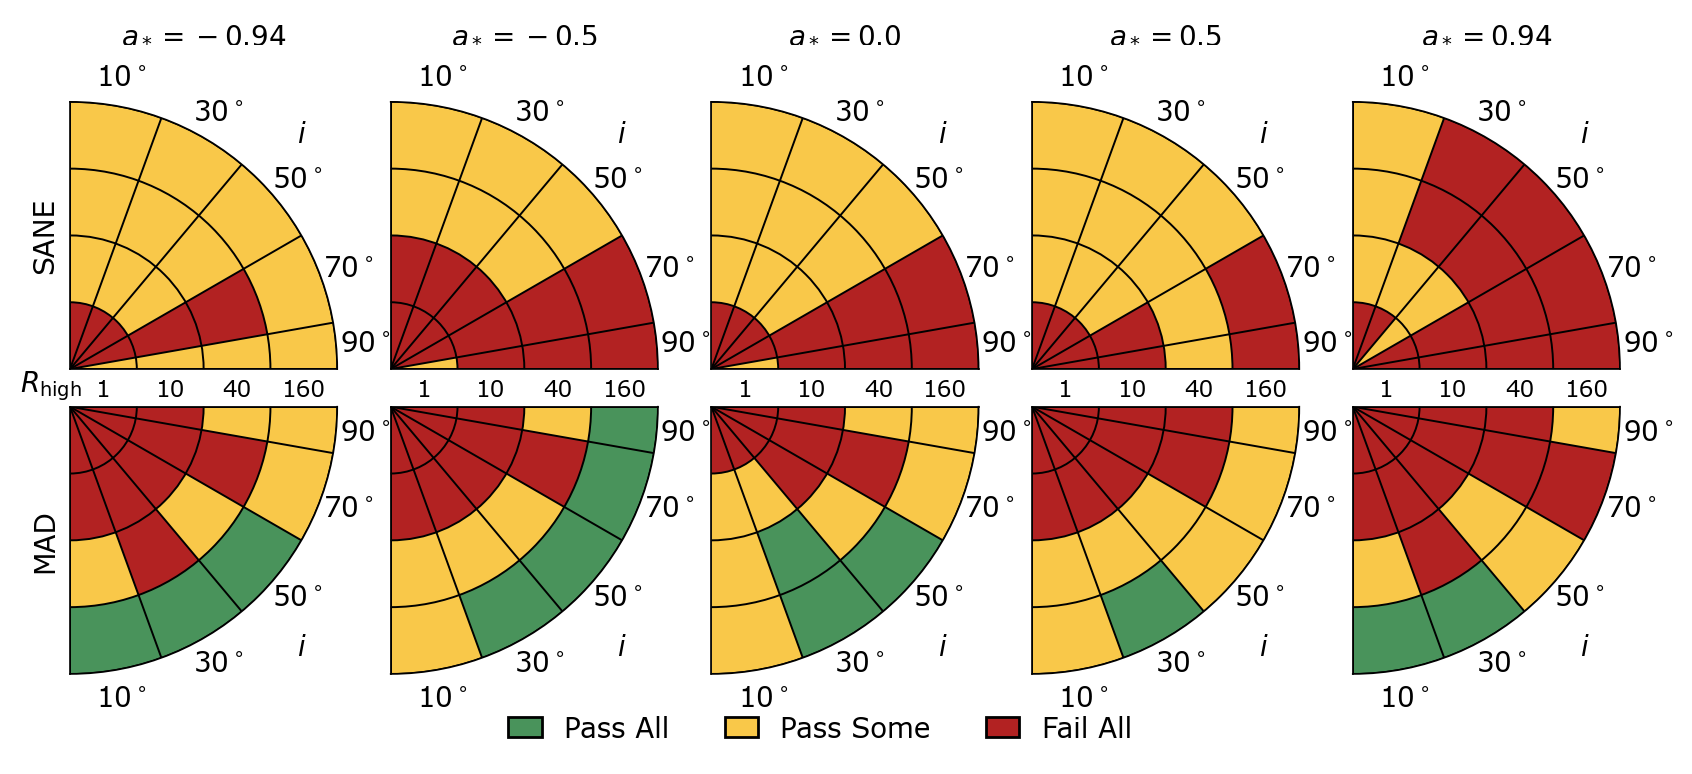
\includegraphics[width=0.8\textwidth]{./figures/Non_Interferometric_Constraints.png}
  \caption{Combined non-EHT Constraints}
  \label{fig:noneht_pizza}
\end{figure*}

Then the full set of combined constraints, without variability.

\begin{figure*}
  \centering
  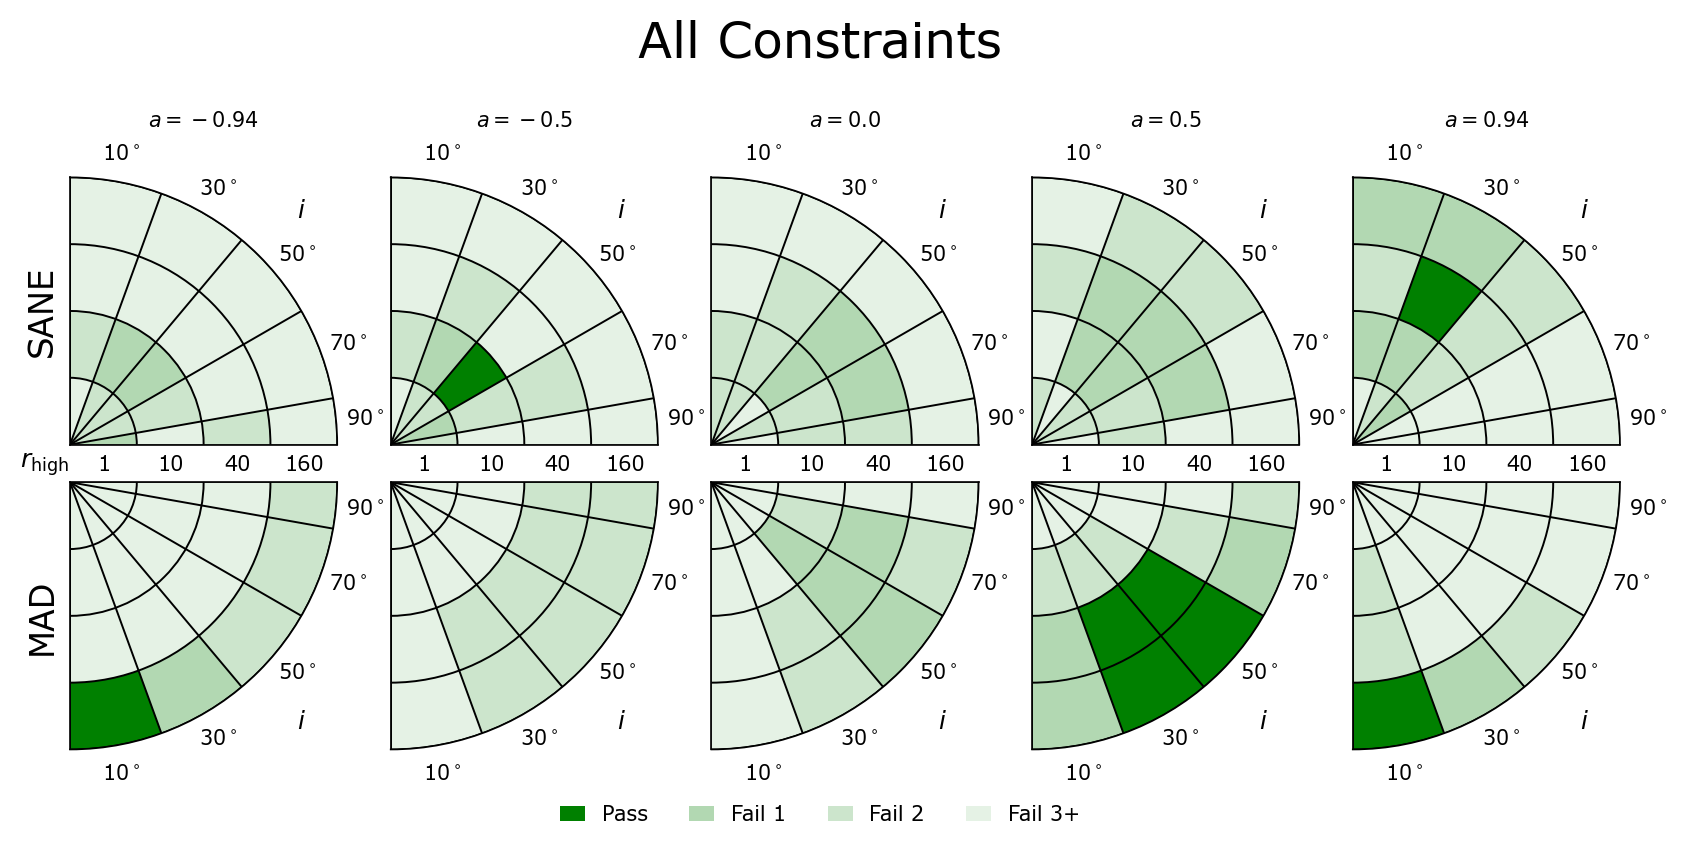
\includegraphics[width=0.8\textwidth]{./figures/All_Constraints.png}
  \caption{Combined Constraints}
  \label{fig:all_pizza}
\end{figure*}

\clearpage

\startlongtable
\begin{deluxetable*}{cccc|cccc|c|ccccc|c|c|cc|cccc}
\tabletypesize{\scriptsize}
\tablecaption{Pass/Fail Table, Illinois Thermal Models}
\label{tab:illinoisPF}
\tablehead{ \colhead{M/S}  &  %
\colhead{Spin}  &  %
\colhead{$i$}  &  %
\colhead{$\Rh$}  &  %
\colhead{$F_{86}$}  &  %
\colhead{$\lambda_{maj,86}$}  &  %
\colhead{$F_{2\mu{\rm m}}$}  &  %
\colhead{$L_X$}  &  %
\colhead{non-EHT}  &  %
\colhead{$\lambda_{230}$}  &  %
\colhead{Nulls}  &  %
\colhead{Ring D}  &  %
\colhead{Ring W}  &  %
\colhead{Ring A}  &  %
\colhead{EHT}  &  %
\colhead{All}  &  %
\colhead{MI} & %
\colhead{4G$\lambda$} & %
\colhead{$\dot{M}/\dot{M}_{Edd}$}  &  %
\colhead{$L_{bol}/(\dot{M} c^{2})$}  &  %
\colhead{$P_{out}$(cgs)}  &  %
\colhead{$P_{out}/(\dot{M} c^2)$}}
\startdata
S & -0.94 & 10.0 & 1.0 & Fail & Fail & Pass & Pass & Fail & Fail & Pass & Pass & Fail & Pass & Fail & Fail & Pass & Pass &1.75$\times10^{-7}$ & 1.33$\times10^{-4}$ & 2.21$\times10^{36}$ & 2.46$\times10^{-3}$\\
S & -0.94 & 10.0 & 10.0 & Pass & Pass & Pass & Fail & Fail & Pass & Pass & Fail & Fail & Pass & Fail & Fail & Fail & Fail &2.09$\times10^{-6}$ & 3.35$\times10^{-5}$ & 2.67$\times10^{37}$ & 2.46$\times10^{-3}$\\
S & -0.94 & 10.0 & 40.0 & Pass & Fail & Pass & Fail & Fail & Pass & Pass & Fail & Fail & Pass & Fail & Fail & Fail & Pass &7.75$\times10^{-6}$ & 2.40$\times10^{-5}$ & 9.90$\times10^{37}$ & 2.46$\times10^{-3}$\\
S & -0.94 & 10.0 & 160.0 & Pass & Fail & Pass & Fail & Fail & Pass & Pass & Fail & Fail & Pass & Fail & Fail & Fail & Pass &1.35$\times10^{-5}$ & 1.19$\times10^{-5}$ & 1.71$\times10^{38}$ & 2.46$\times10^{-3}$\\
S & -0.94 & 30.0 & 1.0 & Fail & Pass & Pass & Pass & Fail & Pass & Pass & Pass & Fail & Pass & Fail & Fail & Fail & Pass &1.68$\times10^{-7}$ & 1.28$\times10^{-4}$ & 2.12$\times10^{36}$ & 2.46$\times10^{-3}$\\
S & -0.94 & 30.0 & 10.0 & Pass & Pass & Pass & Fail & Fail & Pass & Pass & Pass & Fail & Pass & Fail & Fail & Fail & Fail &2.01$\times10^{-6}$ & 3.22$\times10^{-5}$ & 2.56$\times10^{37}$ & 2.46$\times10^{-3}$\\
S & -0.94 & 30.0 & 40.0 & Pass & Pass & Pass & Fail & Fail & Pass & Pass & Fail & Pass & Pass & Fail & Fail & Fail & Pass &8.14$\times10^{-6}$ & 2.53$\times10^{-5}$ & 1.04$\times10^{38}$ & 2.46$\times10^{-3}$\\
S & -0.94 & 30.0 & 160.0 & Pass & Pass & Pass & Fail & Fail & Pass & Pass & Fail & Fail & Pass & Fail & Fail & Fail & Pass &1.48$\times10^{-5}$ & 1.29$\times10^{-5}$ & 1.86$\times10^{38}$ & 2.46$\times10^{-3}$\\
S & -0.94 & 50.0 & 1.0 & Fail & Pass & Pass & Pass & Fail & Pass & Pass & Pass & Fail & Pass & Fail & Fail & Fail & Fail &1.64$\times10^{-7}$ & 1.25$\times10^{-4}$ & 2.06$\times10^{36}$ & 2.46$\times10^{-3}$\\
S & -0.94 & 50.0 & 10.0 & Pass & Pass & Pass & Fail & Fail & Pass & Pass & Pass & Fail & Pass & Fail & Fail & Fail & Fail &1.98$\times10^{-6}$ & 3.18$\times10^{-5}$ & 2.53$\times10^{37}$ & 2.46$\times10^{-3}$\\
S & -0.94 & 50.0 & 40.0 & Pass & Fail & Fail & Fail & Fail & Pass & Pass & Fail & Fail & Pass & Fail & Fail & Fail & Pass &8.47$\times10^{-6}$ & 2.62$\times10^{-5}$ & 1.08$\times10^{38}$ & 2.46$\times10^{-3}$\\
S & -0.94 & 50.0 & 160.0 & Pass & Fail & Pass & Fail & Fail & Pass & Pass & Pass & Fail & Pass & Fail & Fail & Fail & Fail &1.57$\times10^{-5}$ & 1.37$\times10^{-5}$ & 1.99$\times10^{38}$ & 2.46$\times10^{-3}$\\
S & -0.94 & 70.0 & 1.0 & Fail & Pass & Pass & Pass & Fail & Pass & Pass & Pass & Fail & Pass & Fail & Fail & Fail & Fail &1.71$\times10^{-7}$ & 1.30$\times10^{-4}$ & 2.15$\times10^{36}$ & 2.46$\times10^{-3}$\\
S & -0.94 & 70.0 & 10.0 & Pass & Pass & Pass & Fail & Fail & Pass & Pass & Fail & Fail & Pass & Fail & Fail & Fail & Fail &2.19$\times10^{-6}$ & 3.50$\times10^{-5}$ & 2.80$\times10^{37}$ & 2.46$\times10^{-3}$\\
S & -0.94 & 70.0 & 40.0 & Pass & Fail & Fail & Fail & Fail & Pass & Pass & Pass & Fail & Pass & Fail & Fail & Fail & Fail &8.78$\times10^{-6}$ & 2.71$\times10^{-5}$ & 1.12$\times10^{38}$ & 2.46$\times10^{-3}$\\
S & -0.94 & 70.0 & 160.0 & Pass & Fail & Pass & Fail & Fail & Pass & Pass & Pass & Fail & Pass & Fail & Fail & Fail & Fail &1.68$\times10^{-5}$ & 1.47$\times10^{-5}$ & 2.12$\times10^{38}$ & 2.46$\times10^{-3}$\\
S & -0.94 & 90.0 & 1.0 & Fail & Pass & Pass & Pass & Fail & Pass & Pass & Pass & Pass & Pass & Pass & Fail & Fail & Pass &1.71$\times10^{-7}$ & 1.30$\times10^{-4}$ & 2.15$\times10^{36}$ & 2.46$\times10^{-3}$\\
S & -0.94 & 90.0 & 10.0 & Fail & Pass & Pass & Fail & Fail & Pass & Pass & Fail & Fail & Pass & Fail & Fail & Fail & Pass &2.29$\times10^{-6}$ & 3.64$\times10^{-5}$ & 2.92$\times10^{37}$ & 2.46$\times10^{-3}$\\
S & -0.94 & 90.0 & 40.0 & Pass & Fail & Fail & Fail & Fail & Pass & Pass & Pass & Pass & Pass & Pass & Fail & Fail & Fail &9.16$\times10^{-6}$ & 2.82$\times10^{-5}$ & 1.17$\times10^{38}$ & 2.46$\times10^{-3}$\\
S & -0.94 & 90.0 & 160.0 & Pass & Fail & Pass & Fail & Fail & Pass & Pass & Pass & Fail & Pass & Fail & Fail & Fail & Fail &1.79$\times10^{-5}$ & 1.56$\times10^{-5}$ & 2.27$\times10^{38}$ & 2.46$\times10^{-3}$\\
S & -0.5 & 10.0 & 1.0 & Fail & Pass & Pass & Pass & Fail & Fail & Pass & Pass & Fail & Pass & Fail & Fail & Pass & Pass &1.05$\times10^{-7}$ & 2.26$\times10^{-4}$ & 1.89$\times10^{35}$ & 3.53$\times10^{-4}$\\
S & -0.5 & 10.0 & 10.0 & Pass & Pass & Pass & Fail & Fail & Pass & Pass & Fail & Fail & Pass & Fail & Fail & Fail & Fail &1.16$\times10^{-6}$ & 3.65$\times10^{-5}$ & 2.08$\times10^{36}$ & 3.53$\times10^{-4}$\\
S & -0.5 & 10.0 & 40.0 & Pass & Fail & Pass & Fail & Fail & Pass & Pass & Fail & Pass & Pass & Fail & Fail & Pass & Pass &6.87$\times10^{-6}$ & 2.84$\times10^{-5}$ & 1.18$\times10^{37}$ & 3.53$\times10^{-4}$\\
S & -0.5 & 10.0 & 160.0 & Pass & Fail & Pass & Fail & Fail & Pass & Pass & Fail & Pass & Pass & Fail & Fail & Pass & Pass &1.11$\times10^{-5}$ & 1.25$\times10^{-5}$ & 1.90$\times10^{37}$ & 3.53$\times10^{-4}$\\
S & -0.5 & 30.0 & 1.0 & Fail & Pass & Pass & Pass & Fail & Pass & Pass & Pass & Fail & Pass & Fail & Fail & Fail & Pass &1.01$\times10^{-7}$ & 2.17$\times10^{-4}$ & 1.81$\times10^{35}$ & 3.53$\times10^{-4}$\\
S & -0.5 & 30.0 & 10.0 & Pass & Pass & Pass & Fail & Fail & Pass & Pass & Pass & Fail & Pass & Fail & Fail & Fail & Fail &1.09$\times10^{-6}$ & 3.46$\times10^{-5}$ & 1.96$\times10^{36}$ & 3.53$\times10^{-4}$\\
S & -0.5 & 30.0 & 40.0 & Pass & Pass & Pass & Fail & Fail & Pass & Pass & Fail & Pass & Pass & Fail & Fail & Pass & Pass &6.93$\times10^{-6}$ & 2.85$\times10^{-5}$ & 1.18$\times10^{37}$ & 3.53$\times10^{-4}$\\
S & -0.5 & 30.0 & 160.0 & Pass & Pass & Pass & Fail & Fail & Pass & Pass & Fail & Fail & Pass & Fail & Fail & Pass & Pass &1.13$\times10^{-5}$ & 1.26$\times10^{-5}$ & 1.92$\times10^{37}$ & 3.53$\times10^{-4}$\\
S & -0.5 & 50.0 & 1.0 & Fail & Pass & Pass & Pass & Fail & Pass & Pass & Pass & Fail & Pass & Fail & Fail & Fail & Pass &9.75$\times10^{-8}$ & 2.11$\times10^{-4}$ & 1.75$\times10^{35}$ & 3.53$\times10^{-4}$\\
S & -0.5 & 50.0 & 10.0 & Pass & Pass & Pass & Fail & Fail & Pass & Pass & Pass & Fail & Pass & Fail & Fail & Fail & Fail &1.10$\times10^{-6}$ & 3.48$\times10^{-5}$ & 1.97$\times10^{36}$ & 3.53$\times10^{-4}$\\
S & -0.5 & 50.0 & 40.0 & Pass & Fail & Pass & Fail & Fail & Pass & Pass & Fail & Fail & Pass & Fail & Fail & Pass & Pass &6.55$\times10^{-6}$ & 2.70$\times10^{-5}$ & 1.12$\times10^{37}$ & 3.53$\times10^{-4}$\\
S & -0.5 & 50.0 & 160.0 & Pass & Pass & Pass & Fail & Fail & Pass & Fail & Fail & Fail & Pass & Fail & Fail & Pass & Pass &1.10$\times10^{-5}$ & 1.22$\times10^{-5}$ & 1.85$\times10^{37}$ & 3.53$\times10^{-4}$\\
S & -0.5 & 70.0 & 1.0 & Fail & Pass & Pass & Pass & Fail & Pass & Pass & Pass & Pass & Pass & Pass & Fail & Fail & Fail &9.96$\times10^{-8}$ & 2.14$\times10^{-4}$ & 1.78$\times10^{35}$ & 3.53$\times10^{-4}$\\
S & -0.5 & 70.0 & 10.0 & Fail & Pass & Pass & Fail & Fail & Pass & Pass & Pass & Fail & Pass & Fail & Fail & Fail & Fail &1.18$\times10^{-6}$ & 3.71$\times10^{-5}$ & 2.12$\times10^{36}$ & 3.53$\times10^{-4}$\\
S & -0.5 & 70.0 & 40.0 & Pass & Fail & Pass & Fail & Fail & Pass & Pass & Pass & Pass & Pass & Pass & Fail & Pass & Pass &6.41$\times10^{-6}$ & 2.63$\times10^{-5}$ & 1.08$\times10^{37}$ & 3.53$\times10^{-4}$\\
S & -0.5 & 70.0 & 160.0 & Pass & Fail & Pass & Fail & Fail & Pass & Fail & Pass & Fail & Pass & Fail & Fail & Pass & Fail &1.13$\times10^{-5}$ & 1.24$\times10^{-5}$ & 1.89$\times10^{37}$ & 3.53$\times10^{-4}$\\
S & -0.5 & 90.0 & 1.0 & Fail & Fail & Pass & Pass & Fail & Pass & Pass & Pass & Pass & Pass & Pass & Fail & Fail & Pass &1.00$\times10^{-7}$ & 2.15$\times10^{-4}$ & 1.79$\times10^{35}$ & 3.53$\times10^{-4}$\\
S & -0.5 & 90.0 & 10.0 & Fail & Pass & Pass & Fail & Fail & Pass & Pass & Pass & Fail & Pass & Fail & Fail & Fail & Pass &1.27$\times10^{-6}$ & 3.96$\times10^{-5}$ & 2.27$\times10^{36}$ & 3.53$\times10^{-4}$\\
S & -0.5 & 90.0 & 40.0 & Pass & Fail & Pass & Fail & Fail & Pass & Fail & Pass & Pass & Pass & Fail & Fail & Fail & Fail &6.36$\times10^{-6}$ & 2.61$\times10^{-5}$ & 1.08$\times10^{37}$ & 3.53$\times10^{-4}$\\
S & -0.5 & 90.0 & 160.0 & Pass & Fail & Pass & Fail & Fail & Pass & Fail & Pass & Fail & Pass & Fail & Fail & Pass & Fail &1.14$\times10^{-5}$ & 1.24$\times10^{-5}$ & 1.89$\times10^{37}$ & 3.53$\times10^{-4}$\\
S & 0.0 & 10.0 & 1.0 & Fail & Pass & Pass & Pass & Fail & Fail & Pass & Pass & Fail & Pass & Fail & Fail & Pass & Pass &5.80$\times10^{-8}$ & 4.53$\times10^{-4}$ & 1.17$\times10^{35}$ & 3.96$\times10^{-4}$\\
S & 0.0 & 10.0 & 10.0 & Pass & Pass & Pass & Pass & Pass & Pass & Pass & Fail & Fail & Pass & Fail & Fail & Fail & Fail &5.07$\times10^{-7}$ & 6.62$\times10^{-5}$ & 1.05$\times10^{36}$ & 3.96$\times10^{-4}$\\
S & 0.0 & 10.0 & 40.0 & Fail & Fail & Pass & Fail & Fail & Pass & Fail & Fail & Pass & Pass & Fail & Fail & Fail & Pass &2.70$\times10^{-6}$ & 3.91$\times10^{-5}$ & 5.60$\times10^{36}$ & 3.96$\times10^{-4}$\\
S & 0.0 & 10.0 & 160.0 & Pass & Fail & Pass & Fail & Fail & Pass & Fail & Fail & Pass & Pass & Fail & Fail & Fail & Pass &4.62$\times10^{-6}$ & 1.69$\times10^{-5}$ & 8.94$\times10^{36}$ & 3.96$\times10^{-4}$\\
S & 0.0 & 30.0 & 1.0 & Fail & Pass & Pass & Pass & Fail & Pass & Pass & Pass & Fail & Pass & Fail & Fail & Fail & Pass &5.50$\times10^{-8}$ & 4.32$\times10^{-4}$ & 1.11$\times10^{35}$ & 3.96$\times10^{-4}$\\
S & 0.0 & 30.0 & 10.0 & Pass & Fail & Pass & Pass & Fail & Pass & Pass & Pass & Fail & Pass & Fail & Fail & Fail & Fail &4.79$\times10^{-7}$ & 6.29$\times10^{-5}$ & 9.93$\times10^{35}$ & 3.96$\times10^{-4}$\\
S & 0.0 & 30.0 & 40.0 & Fail & Fail & Pass & Fail & Fail & Pass & Pass & Fail & Pass & Pass & Fail & Fail & Fail & Pass &2.60$\times10^{-6}$ & 3.79$\times10^{-5}$ & 5.36$\times10^{36}$ & 3.96$\times10^{-4}$\\
S & 0.0 & 30.0 & 160.0 & Pass & Fail & Pass & Fail & Fail & Pass & Pass & Fail & Fail & Pass & Fail & Fail & Fail & Pass &4.32$\times10^{-6}$ & 1.59$\times10^{-5}$ & 8.38$\times10^{36}$ & 3.96$\times10^{-4}$\\
S & 0.0 & 50.0 & 1.0 & Fail & Fail & Pass & Pass & Fail & Pass & Pass & Pass & Fail & Pass & Fail & Fail & Fail & Pass &5.29$\times10^{-8}$ & 4.16$\times10^{-4}$ & 1.06$\times10^{35}$ & 3.96$\times10^{-4}$\\
S & 0.0 & 50.0 & 10.0 & Pass & Fail & Pass & Pass & Fail & Pass & Pass & Pass & Pass & Pass & Pass & Fail & Fail & Fail &4.66$\times10^{-7}$ & 6.13$\times10^{-5}$ & 9.67$\times10^{35}$ & 3.96$\times10^{-4}$\\
S & 0.0 & 50.0 & 40.0 & Pass & Pass & Pass & Fail & Fail & Pass & Pass & Pass & Pass & Pass & Pass & Fail & Fail & Fail &2.72$\times10^{-6}$ & 3.96$\times10^{-5}$ & 5.69$\times10^{36}$ & 3.96$\times10^{-4}$\\
S & 0.0 & 50.0 & 160.0 & Pass & Pass & Pass & Fail & Fail & Pass & Pass & Pass & Fail & Pass & Fail & Fail & Pass & Pass &4.71$\times10^{-6}$ & 1.73$\times10^{-5}$ & 9.32$\times10^{36}$ & 3.96$\times10^{-4}$\\
S & 0.0 & 70.0 & 1.0 & Fail & Fail & Pass & Pass & Fail & Pass & Pass & Pass & Pass & Pass & Pass & Fail & Fail & Pass &5.33$\times10^{-8}$ & 4.19$\times10^{-4}$ & 1.07$\times10^{35}$ & 3.96$\times10^{-4}$\\
S & 0.0 & 70.0 & 10.0 & Fail & Fail & Pass & Pass & Fail & Pass & Pass & Pass & Pass & Pass & Pass & Fail & Fail & Fail &4.96$\times10^{-7}$ & 6.48$\times10^{-5}$ & 1.04$\times10^{36}$ & 3.96$\times10^{-4}$\\
S & 0.0 & 70.0 & 40.0 & Pass & Fail & Pass & Fail & Fail & Pass & Pass & Pass & Pass & Pass & Pass & Fail & Fail & Fail &2.80$\times10^{-6}$ & 4.07$\times10^{-5}$ & 5.88$\times10^{36}$ & 3.96$\times10^{-4}$\\
S & 0.0 & 70.0 & 160.0 & Pass & Fail & Pass & Fail & Fail & Pass & Fail & Pass & Fail & Pass & Fail & Fail & Pass & Pass &4.84$\times10^{-6}$ & 1.77$\times10^{-5}$ & 9.72$\times10^{36}$ & 3.96$\times10^{-4}$\\
S & 0.0 & 90.0 & 1.0 & Fail & Fail & Pass & Pass & Fail & Pass & Pass & Pass & Fail & Pass & Fail & Fail & Fail & Pass &5.33$\times10^{-8}$ & 4.18$\times10^{-4}$ & 1.07$\times10^{35}$ & 3.96$\times10^{-4}$\\
S & 0.0 & 90.0 & 10.0 & Fail & Fail & Pass & Pass & Fail & Pass & Pass & Pass & Pass & Pass & Pass & Fail & Fail & Fail &5.20$\times10^{-7}$ & 6.76$\times10^{-5}$ & 1.09$\times10^{36}$ & 3.96$\times10^{-4}$\\
S & 0.0 & 90.0 & 40.0 & Pass & Fail & Pass & Fail & Fail & Pass & Pass & Pass & Pass & Pass & Pass & Fail & Fail & Fail &2.77$\times10^{-6}$ & 4.04$\times10^{-5}$ & 5.88$\times10^{36}$ & 3.96$\times10^{-4}$\\
S & 0.0 & 90.0 & 160.0 & Pass & Fail & Pass & Fail & Fail & Pass & Fail & Pass & Pass & Pass & Fail & Fail & Pass & Pass &4.88$\times10^{-6}$ & 1.79$\times10^{-5}$ & 9.87$\times10^{36}$ & 3.96$\times10^{-4}$\\
S & 0.5 & 10.0 & 1.0 & Fail & Pass & Pass & Pass & Fail & Pass & Pass & Pass & Fail & Pass & Fail & Fail & Pass & Pass &2.62$\times10^{-8}$ & 1.15$\times10^{-3}$ & 1.10$\times10^{35}$ & 8.37$\times10^{-4}$\\
S & 0.5 & 10.0 & 10.0 & Pass & Fail & Pass & Pass & Fail & Pass & Pass & Fail & Fail & Pass & Fail & Fail & Fail & Pass &2.11$\times10^{-7}$ & 1.61$\times10^{-4}$ & 8.95$\times10^{35}$ & 8.37$\times10^{-4}$\\
S & 0.5 & 10.0 & 40.0 & Fail & Fail & Pass & Fail & Fail & Pass & Pass & Pass & Pass & Pass & Pass & Fail & Pass & Pass &2.49$\times10^{-6}$ & 9.77$\times10^{-5}$ & 9.45$\times10^{36}$ & 8.37$\times10^{-4}$\\
S & 0.5 & 10.0 & 160.0 & Pass & Fail & Pass & Fail & Fail & Pass & Pass & Fail & Pass & Pass & Fail & Fail & Fail & Pass &5.67$\times10^{-6}$ & 3.65$\times10^{-5}$ & 2.20$\times10^{37}$ & 8.37$\times10^{-4}$\\
S & 0.5 & 30.0 & 1.0 & Fail & Pass & Pass & Pass & Fail & Pass & Pass & Pass & Fail & Pass & Fail & Fail & Pass & Pass &2.50$\times10^{-8}$ & 1.10$\times10^{-3}$ & 1.05$\times10^{35}$ & 8.37$\times10^{-4}$\\
S & 0.5 & 30.0 & 10.0 & Pass & Fail & Pass & Pass & Fail & Pass & Pass & Pass & Pass & Pass & Pass & Fail & Fail & Pass &2.01$\times10^{-7}$ & 1.52$\times10^{-4}$ & 8.44$\times10^{35}$ & 8.37$\times10^{-4}$\\
S & 0.5 & 30.0 & 40.0 & Fail & Pass & Pass & Fail & Fail & Pass & Pass & Pass & Pass & Pass & Pass & Fail & Pass & Pass &2.66$\times10^{-6}$ & 1.08$\times10^{-4}$ & 1.02$\times10^{37}$ & 8.37$\times10^{-4}$\\
S & 0.5 & 30.0 & 160.0 & Pass & Pass & Pass & Fail & Fail & Pass & Pass & Fail & Pass & Pass & Fail & Fail & Fail & Pass &5.73$\times10^{-6}$ & 3.86$\times10^{-5}$ & 2.27$\times10^{37}$ & 8.37$\times10^{-4}$\\
S & 0.5 & 50.0 & 1.0 & Fail & Fail & Pass & Pass & Fail & Pass & Pass & Pass & Pass & Pass & Pass & Fail & Fail & Pass &2.39$\times10^{-8}$ & 1.05$\times10^{-3}$ & 1.01$\times10^{35}$ & 8.37$\times10^{-4}$\\
S & 0.5 & 50.0 & 10.0 & Pass & Fail & Pass & Pass & Fail & Pass & Pass & Pass & Pass & Pass & Pass & Fail & Fail & Pass &1.94$\times10^{-7}$ & 1.47$\times10^{-4}$ & 8.18$\times10^{35}$ & 8.37$\times10^{-4}$\\
S & 0.5 & 50.0 & 40.0 & Fail & Pass & Pass & Fail & Fail & Pass & Pass & Pass & Pass & Pass & Pass & Fail & Pass & Pass &2.91$\times10^{-6}$ & 1.19$\times10^{-4}$ & 1.13$\times10^{37}$ & 8.37$\times10^{-4}$\\
S & 0.5 & 50.0 & 160.0 & Pass & Pass & Pass & Fail & Fail & Pass & Pass & Pass & Fail & Pass & Fail & Fail & Fail & Fail &6.23$\times10^{-6}$ & 4.15$\times10^{-5}$ & 2.47$\times10^{37}$ & 8.37$\times10^{-4}$\\
S & 0.5 & 70.0 & 1.0 & Fail & Fail & Pass & Pass & Fail & Pass & Pass & Pass & Pass & Pass & Pass & Fail & Fail & Pass &2.38$\times10^{-8}$ & 1.04$\times10^{-3}$ & 1.00$\times10^{35}$ & 8.37$\times10^{-4}$\\
S & 0.5 & 70.0 & 10.0 & Fail & Fail & Pass & Pass & Fail & Pass & Pass & Pass & Pass & Pass & Pass & Fail & Pass & Pass &2.02$\times10^{-7}$ & 1.54$\times10^{-4}$ & 8.56$\times10^{35}$ & 8.37$\times10^{-4}$\\
S & 0.5 & 70.0 & 40.0 & Fail & Pass & Fail & Fail & Fail & Pass & Pass & Pass & Pass & Pass & Pass & Fail & Pass & Pass &3.04$\times10^{-6}$ & 1.27$\times10^{-4}$ & 1.19$\times10^{37}$ & 8.37$\times10^{-4}$\\
S & 0.5 & 70.0 & 160.0 & Pass & Fail & Pass & Fail & Fail & Pass & Fail & Pass & Fail & Pass & Fail & Fail & Fail & Fail &6.24$\times10^{-6}$ & 4.12$\times10^{-5}$ & 2.47$\times10^{37}$ & 8.37$\times10^{-4}$\\
S & 0.5 & 90.0 & 1.0 & Fail & Fail & Pass & Pass & Fail & Pass & Fail & Pass & Pass & Pass & Fail & Fail & Fail & Pass &2.36$\times10^{-8}$ & 1.03$\times10^{-3}$ & 9.91$\times10^{34}$ & 8.37$\times10^{-4}$\\
S & 0.5 & 90.0 & 10.0 & Fail & Fail & Pass & Pass & Fail & Pass & Pass & Pass & Pass & Pass & Pass & Fail & Pass & Pass &2.24$\times10^{-7}$ & 1.67$\times10^{-4}$ & 9.43$\times10^{35}$ & 8.37$\times10^{-4}$\\
S & 0.5 & 90.0 & 40.0 & Fail & Pass & Fail & Fail & Fail & Pass & Pass & Pass & Pass & Pass & Pass & Fail & Pass & Fail &2.94$\times10^{-6}$ & 1.25$\times10^{-4}$ & 1.15$\times10^{37}$ & 8.37$\times10^{-4}$\\
S & 0.5 & 90.0 & 160.0 & Pass & Fail & Pass & Fail & Fail & Pass & Fail & Pass & Fail & Pass & Fail & Fail & Fail & Fail &6.07$\times10^{-6}$ & 4.01$\times10^{-5}$ & 2.40$\times10^{37}$ & 8.37$\times10^{-4}$\\
S & 0.94 & 10.0 & 1.0 & Fail & Fail & Pass & Pass & Fail & Pass & Pass & Fail & Fail & Pass & Fail & Fail & Pass & Pass &8.76$\times10^{-9}$ & 7.98$\times10^{-3}$ & 1.96$\times10^{36}$ & 4.32$\times10^{-2}$\\
S & 0.94 & 10.0 & 10.0 & Pass & Fail & Pass & Pass & Fail & Pass & Pass & Pass & Pass & Pass & Pass & Fail & Fail & Pass &4.65$\times10^{-8}$ & 1.75$\times10^{-3}$ & 1.04$\times10^{37}$ & 4.32$\times10^{-2}$\\
S & 0.94 & 10.0 & 40.0 & Pass & Fail & Pass & Pass & Fail & Pass & Pass & Pass & Pass & Pass & Pass & Fail & Pass & Pass &3.37$\times10^{-7}$ & 9.72$\times10^{-4}$ & 6.94$\times10^{37}$ & 4.32$\times10^{-2}$\\
S & 0.94 & 10.0 & 160.0 & Pass & Fail & Pass & Pass & Fail & Pass & Pass & Pass & Pass & Pass & Pass & Fail & Fail & Pass &6.95$\times10^{-7}$ & 3.66$\times10^{-4}$ & 1.38$\times10^{38}$ & 4.32$\times10^{-2}$\\
S & 0.94 & 30.0 & 1.0 & Fail & Fail & Pass & Pass & Fail & Pass & Pass & Pass & Pass & Pass & Pass & Fail & Pass & Pass &8.25$\times10^{-9}$ & 7.48$\times10^{-3}$ & 1.85$\times10^{36}$ & 4.32$\times10^{-2}$\\
S & 0.94 & 30.0 & 10.0 & Pass & Fail & Pass & Pass & Fail & Pass & Pass & Pass & Pass & Pass & Pass & Fail & Fail & Pass &4.37$\times10^{-8}$ & 1.64$\times10^{-3}$ & 9.69$\times10^{36}$ & 4.32$\times10^{-2}$\\
S & 0.94 & 30.0 & 40.0 & Pass & Fail & Pass & Pass & Fail & Pass & Pass & Pass & Pass & Pass & Pass & Fail & Pass & Pass &3.53$\times10^{-7}$ & 1.00$\times10^{-3}$ & 7.16$\times10^{37}$ & 4.32$\times10^{-2}$\\
S & 0.94 & 30.0 & 160.0 & Pass & Fail & Pass & Pass & Fail & Pass & Pass & Pass & Pass & Pass & Pass & Fail & Fail & Pass &7.03$\times10^{-7}$ & 3.73$\times10^{-4}$ & 1.41$\times10^{38}$ & 4.32$\times10^{-2}$\\
S & 0.94 & 50.0 & 1.0 & Pass & Fail & Pass & Pass & Fail & Pass & Pass & Pass & Pass & Pass & Pass & Fail & Pass & Pass &7.72$\times10^{-9}$ & 6.97$\times10^{-3}$ & 1.73$\times10^{36}$ & 4.32$\times10^{-2}$\\
S & 0.94 & 50.0 & 10.0 & Pass & Fail & Pass & Pass & Fail & Pass & Pass & Pass & Pass & Fail & Fail & Fail & Fail & Fail &3.93$\times10^{-8}$ & 1.48$\times10^{-3}$ & 8.75$\times10^{36}$ & 4.32$\times10^{-2}$\\
S & 0.94 & 50.0 & 40.0 & Pass & Fail & Fail & Fail & Fail & Pass & Pass & Pass & Pass & Pass & Pass & Fail & Pass & Pass &3.68$\times10^{-7}$ & 1.04$\times10^{-3}$ & 7.47$\times10^{37}$ & 4.32$\times10^{-2}$\\
S & 0.94 & 50.0 & 160.0 & Pass & Fail & Fail & Fail & Fail & Pass & Pass & Pass & Pass & Pass & Pass & Fail & Pass & Fail &7.94$\times10^{-7}$ & 4.15$\times10^{-4}$ & 1.57$\times10^{38}$ & 4.32$\times10^{-2}$\\
S & 0.94 & 70.0 & 1.0 & Pass & Fail & Pass & Fail & Fail & Pass & Fail & Pass & Pass & Pass & Fail & Fail & Pass & Pass &7.54$\times10^{-9}$ & 6.79$\times10^{-3}$ & 1.69$\times10^{36}$ & 4.32$\times10^{-2}$\\
S & 0.94 & 70.0 & 10.0 & Fail & Fail & Pass & Pass & Fail & Pass & Fail & Pass & Pass & Fail & Fail & Fail & Pass & Fail &3.89$\times10^{-8}$ & 1.46$\times10^{-3}$ & 8.63$\times10^{36}$ & 4.32$\times10^{-2}$\\
S & 0.94 & 70.0 & 40.0 & Pass & Fail & Fail & Fail & Fail & Pass & Pass & Pass & Pass & Pass & Pass & Fail & Pass & Fail &3.83$\times10^{-7}$ & 1.09$\times10^{-3}$ & 7.77$\times10^{37}$ & 4.32$\times10^{-2}$\\
S & 0.94 & 70.0 & 160.0 & Pass & Fail & Fail & Fail & Fail & Pass & Fail & Pass & Fail & Pass & Fail & Fail & Pass & Pass &8.51$\times10^{-7}$ & 4.42$\times10^{-4}$ & 1.68$\times10^{38}$ & 4.32$\times10^{-2}$\\
S & 0.94 & 90.0 & 1.0 & Pass & Fail & Pass & Fail & Fail & Pass & Fail & Pass & Fail & Pass & Fail & Fail & Pass & Pass &7.35$\times10^{-9}$ & 6.62$\times10^{-3}$ & 1.65$\times10^{36}$ & 4.32$\times10^{-2}$\\
S & 0.94 & 90.0 & 10.0 & Fail & Fail & Pass & Pass & Fail & Pass & Fail & Pass & Fail & Fail & Fail & Fail & Pass & Fail &4.11$\times10^{-8}$ & 1.52$\times10^{-3}$ & 9.02$\times10^{36}$ & 4.32$\times10^{-2}$\\
S & 0.94 & 90.0 & 40.0 & Fail & Fail & Fail & Fail & Fail & Pass & Fail & Pass & Fail & Pass & Fail & Fail & Pass & Fail &3.88$\times10^{-7}$ & 1.10$\times10^{-3}$ & 7.88$\times10^{37}$ & 4.32$\times10^{-2}$\\
S & 0.94 & 90.0 & 160.0 & Pass & Fail & Fail & Fail & Fail & Pass & Fail & Pass & Fail & Pass & Fail & Fail & Pass & Pass &8.65$\times10^{-7}$ & 4.53$\times10^{-4}$ & 1.72$\times10^{38}$ & 4.32$\times10^{-2}$\\
M & -0.94 & 10.0 & 1.0 & Fail & Pass & Fail & Fail & Fail & Pass & Pass & Fail & Fail & Pass & Fail & Fail & Fail & Pass &5.53$\times10^{-8}$ & 1.43$\times10^{-2}$ & 1.09$\times10^{38}$ & 3.83$\times10^{-1}$\\
M & -0.94 & 10.0 & 10.0 & Pass & Pass & Fail & Fail & Fail & Pass & Pass & Pass & Fail & Pass & Fail & Fail & Fail & Pass &8.85$\times10^{-8}$ & 4.64$\times10^{-3}$ & 1.76$\times10^{38}$ & 3.83$\times10^{-1}$\\
M & -0.94 & 10.0 & 40.0 & Pass & Pass & Fail & Pass & Fail & Pass & Pass & Pass & Fail & Pass & Fail & Fail & Fail & Pass &1.29$\times10^{-7}$ & 1.91$\times10^{-3}$ & 2.56$\times10^{38}$ & 3.83$\times10^{-1}$\\
M & -0.94 & 10.0 & 160.0 & Pass & Pass & Pass & Pass & Pass & Pass & Pass & Pass & Pass & Pass & Pass & Pass & Fail & Fail &2.17$\times10^{-7}$ & 6.92$\times10^{-4}$ & 4.30$\times10^{38}$ & 3.83$\times10^{-1}$\\
M & -0.94 & 30.0 & 1.0 & Fail & Pass & Fail & Fail & Fail & Pass & Pass & Fail & Fail & Pass & Fail & Fail & Fail & Pass &5.32$\times10^{-8}$ & 1.37$\times10^{-2}$ & 1.05$\times10^{38}$ & 3.83$\times10^{-1}$\\
M & -0.94 & 30.0 & 10.0 & Pass & Pass & Fail & Fail & Fail & Pass & Pass & Pass & Fail & Pass & Fail & Fail & Fail & Fail &8.52$\times10^{-8}$ & 4.46$\times10^{-3}$ & 1.69$\times10^{38}$ & 3.83$\times10^{-1}$\\
M & -0.94 & 30.0 & 40.0 & Pass & Pass & Fail & Pass & Fail & Pass & Pass & Pass & Fail & Pass & Fail & Fail & Fail & Fail &1.24$\times10^{-7}$ & 1.83$\times10^{-3}$ & 2.45$\times10^{38}$ & 3.83$\times10^{-1}$\\
M & -0.94 & 30.0 & 160.0 & Pass & Pass & Pass & Pass & Pass & Pass & Pass & Pass & Fail & Pass & Fail & Fail & Fail & Fail &2.09$\times10^{-7}$ & 6.69$\times10^{-4}$ & 4.15$\times10^{38}$ & 3.83$\times10^{-1}$\\
M & -0.94 & 50.0 & 1.0 & Fail & Pass & Fail & Fail & Fail & Pass & Pass & Fail & Fail & Pass & Fail & Fail & Fail & Pass &4.99$\times10^{-8}$ & 1.26$\times10^{-2}$ & 9.87$\times10^{37}$ & 3.83$\times10^{-1}$\\
M & -0.94 & 50.0 & 10.0 & Fail & Pass & Fail & Fail & Fail & Pass & Pass & Pass & Fail & Pass & Fail & Fail & Fail & Fail &7.78$\times10^{-8}$ & 4.06$\times10^{-3}$ & 1.54$\times10^{38}$ & 3.83$\times10^{-1}$\\
M & -0.94 & 50.0 & 40.0 & Pass & Pass & Fail & Fail & Fail & Pass & Pass & Pass & Fail & Pass & Fail & Fail & Fail & Fail &1.14$\times10^{-7}$ & 1.69$\times10^{-3}$ & 2.27$\times10^{38}$ & 3.83$\times10^{-1}$\\
M & -0.94 & 50.0 & 160.0 & Pass & Pass & Pass & Pass & Pass & Pass & Pass & Pass & Fail & Pass & Fail & Fail & Fail & Fail &1.93$\times10^{-7}$ & 6.20$\times10^{-4}$ & 3.84$\times10^{38}$ & 3.83$\times10^{-1}$\\
M & -0.94 & 70.0 & 1.0 & Fail & Pass & Fail & Fail & Fail & Pass & Pass & Fail & Fail & Pass & Fail & Fail & Fail & Fail &4.60$\times10^{-8}$ & 1.14$\times10^{-2}$ & 9.09$\times10^{37}$ & 3.83$\times10^{-1}$\\
M & -0.94 & 70.0 & 10.0 & Pass & Pass & Fail & Fail & Fail & Pass & Pass & Pass & Fail & Pass & Fail & Fail & Fail & Fail &7.11$\times10^{-8}$ & 3.69$\times10^{-3}$ & 1.41$\times10^{38}$ & 3.83$\times10^{-1}$\\
M & -0.94 & 70.0 & 40.0 & Pass & Pass & Fail & Fail & Fail & Pass & Pass & Pass & Fail & Pass & Fail & Fail & Fail & Fail &1.04$\times10^{-7}$ & 1.54$\times10^{-3}$ & 2.07$\times10^{38}$ & 3.83$\times10^{-1}$\\
M & -0.94 & 70.0 & 160.0 & Pass & Pass & Fail & Pass & Fail & Pass & Pass & Pass & Fail & Pass & Fail & Fail & Fail & Fail &1.76$\times10^{-7}$ & 5.64$\times10^{-4}$ & 3.48$\times10^{38}$ & 3.83$\times10^{-1}$\\
M & -0.94 & 90.0 & 1.0 & Pass & Pass & Fail & Fail & Fail & Pass & Pass & Fail & Fail & Pass & Fail & Fail & Fail & Fail &4.37$\times10^{-8}$ & 1.08$\times10^{-2}$ & 8.61$\times10^{37}$ & 3.83$\times10^{-1}$\\
M & -0.94 & 90.0 & 10.0 & Pass & Pass & Fail & Fail & Fail & Pass & Pass & Pass & Fail & Pass & Fail & Fail & Fail & Fail &6.75$\times10^{-8}$ & 3.50$\times10^{-3}$ & 1.34$\times10^{38}$ & 3.83$\times10^{-1}$\\
M & -0.94 & 90.0 & 40.0 & Pass & Pass & Fail & Fail & Fail & Pass & Pass & Pass & Fail & Pass & Fail & Fail & Fail & Fail &9.99$\times10^{-8}$ & 1.48$\times10^{-3}$ & 1.98$\times10^{38}$ & 3.83$\times10^{-1}$\\
M & -0.94 & 90.0 & 160.0 & Pass & Pass & Fail & Pass & Fail & Pass & Pass & Pass & Fail & Pass & Fail & Fail & Fail & Fail &1.68$\times10^{-7}$ & 5.40$\times10^{-4}$ & 3.34$\times10^{38}$ & 3.83$\times10^{-1}$\\
M & -0.5 & 10.0 & 1.0 & Pass & Pass & Fail & Fail & Fail & Pass & Pass & Fail & Fail & Pass & Fail & Fail & Fail & Pass &4.20$\times10^{-8}$ & 4.91$\times10^{-3}$ & 2.74$\times10^{37}$ & 1.27$\times10^{-1}$\\
M & -0.5 & 10.0 & 10.0 & Pass & Pass & Fail & Fail & Fail & Pass & Pass & Fail & Fail & Pass & Fail & Fail & Fail & Pass &6.98$\times10^{-8}$ & 2.45$\times10^{-3}$ & 4.56$\times10^{37}$ & 1.27$\times10^{-1}$\\
M & -0.5 & 10.0 & 40.0 & Pass & Pass & Pass & Pass & Pass & Pass & Pass & Fail & Fail & Pass & Fail & Fail & Fail & Pass &1.03$\times10^{-7}$ & 1.41$\times10^{-3}$ & 6.71$\times10^{37}$ & 1.27$\times10^{-1}$\\
M & -0.5 & 10.0 & 160.0 & Pass & Fail & Pass & Pass & Fail & Pass & Pass & Fail & Fail & Pass & Fail & Fail & Fail & Pass &1.68$\times10^{-7}$ & 6.60$\times10^{-4}$ & 1.10$\times10^{38}$ & 1.27$\times10^{-1}$\\
M & -0.5 & 30.0 & 1.0 & Pass & Pass & Fail & Fail & Fail & Pass & Pass & Fail & Fail & Pass & Fail & Fail & Fail & Pass &4.09$\times10^{-8}$ & 4.77$\times10^{-3}$ & 2.67$\times10^{37}$ & 1.27$\times10^{-1}$\\
M & -0.5 & 30.0 & 10.0 & Pass & Pass & Fail & Fail & Fail & Pass & Pass & Fail & Fail & Pass & Fail & Fail & Fail & Pass &6.70$\times10^{-8}$ & 2.35$\times10^{-3}$ & 4.38$\times10^{37}$ & 1.27$\times10^{-1}$\\
M & -0.5 & 30.0 & 40.0 & Pass & Pass & Pass & Pass & Pass & Pass & Pass & Fail & Fail & Pass & Fail & Fail & Fail & Pass &9.86$\times10^{-8}$ & 1.35$\times10^{-3}$ & 6.44$\times10^{37}$ & 1.27$\times10^{-1}$\\
M & -0.5 & 30.0 & 160.0 & Pass & Pass & Pass & Pass & Pass & Pass & Pass & Fail & Fail & Pass & Fail & Fail & Fail & Pass &1.62$\times10^{-7}$ & 6.38$\times10^{-4}$ & 1.06$\times10^{38}$ & 1.27$\times10^{-1}$\\
M & -0.5 & 50.0 & 1.0 & Pass & Pass & Fail & Fail & Fail & Pass & Pass & Fail & Fail & Pass & Fail & Fail & Fail & Pass &3.85$\times10^{-8}$ & 4.47$\times10^{-3}$ & 2.52$\times10^{37}$ & 1.27$\times10^{-1}$\\
M & -0.5 & 50.0 & 10.0 & Pass & Pass & Fail & Fail & Fail & Pass & Pass & Pass & Fail & Pass & Fail & Fail & Fail & Pass &6.23$\times10^{-8}$ & 2.19$\times10^{-3}$ & 4.07$\times10^{37}$ & 1.27$\times10^{-1}$\\
M & -0.5 & 50.0 & 40.0 & Pass & Pass & Fail & Pass & Fail & Pass & Pass & Fail & Fail & Pass & Fail & Fail & Fail & Pass &9.24$\times10^{-8}$ & 1.27$\times10^{-3}$ & 6.04$\times10^{37}$ & 1.27$\times10^{-1}$\\
M & -0.5 & 50.0 & 160.0 & Pass & Pass & Pass & Pass & Pass & Pass & Pass & Fail & Fail & Pass & Fail & Fail & Fail & Fail &1.51$\times10^{-7}$ & 5.97$\times10^{-4}$ & 9.89$\times10^{37}$ & 1.27$\times10^{-1}$\\
M & -0.5 & 70.0 & 1.0 & Pass & Pass & Fail & Fail & Fail & Pass & Pass & Fail & Fail & Pass & Fail & Fail & Fail & Pass &3.62$\times10^{-8}$ & 4.18$\times10^{-3}$ & 2.36$\times10^{37}$ & 1.27$\times10^{-1}$\\
M & -0.5 & 70.0 & 10.0 & Pass & Pass & Fail & Fail & Fail & Pass & Pass & Fail & Fail & Pass & Fail & Fail & Fail & Fail &5.72$\times10^{-8}$ & 2.00$\times10^{-3}$ & 3.73$\times10^{37}$ & 1.27$\times10^{-1}$\\
M & -0.5 & 70.0 & 40.0 & Pass & Pass & Fail & Pass & Fail & Pass & Pass & Fail & Fail & Pass & Fail & Fail & Fail & Pass &8.54$\times10^{-8}$ & 1.17$\times10^{-3}$ & 5.57$\times10^{37}$ & 1.27$\times10^{-1}$\\
M & -0.5 & 70.0 & 160.0 & Pass & Pass & Pass & Pass & Pass & Pass & Pass & Fail & Fail & Pass & Fail & Fail & Fail & Fail &1.41$\times10^{-7}$ & 5.56$\times10^{-4}$ & 9.21$\times10^{37}$ & 1.27$\times10^{-1}$\\
M & -0.5 & 90.0 & 1.0 & Pass & Pass & Fail & Fail & Fail & Pass & Fail & Fail & Fail & Pass & Fail & Fail & Fail & Pass &3.36$\times10^{-8}$ & 3.86$\times10^{-3}$ & 2.19$\times10^{37}$ & 1.27$\times10^{-1}$\\
M & -0.5 & 90.0 & 10.0 & Pass & Pass & Fail & Fail & Fail & Pass & Fail & Fail & Fail & Pass & Fail & Fail & Fail & Fail &5.34$\times10^{-8}$ & 1.87$\times10^{-3}$ & 3.49$\times10^{37}$ & 1.27$\times10^{-1}$\\
M & -0.5 & 90.0 & 40.0 & Pass & Pass & Fail & Pass & Fail & Pass & Pass & Fail & Fail & Pass & Fail & Fail & Fail & Fail &8.14$\times10^{-8}$ & 1.12$\times10^{-3}$ & 5.32$\times10^{37}$ & 1.27$\times10^{-1}$\\
M & -0.5 & 90.0 & 160.0 & Pass & Pass & Pass & Pass & Pass & Pass & Pass & Fail & Fail & Pass & Fail & Fail & Fail & Fail &1.35$\times10^{-7}$ & 5.33$\times10^{-4}$ & 8.83$\times10^{37}$ & 1.27$\times10^{-1}$\\
M & 0.0 & 10.0 & 1.0 & Fail & Pass & Fail & Fail & Fail & Pass & Pass & Fail & Fail & Pass & Fail & Fail & Fail & Pass &3.14$\times10^{-8}$ & 5.53$\times10^{-3}$ & 3.70$\times10^{36}$ & 2.27$\times10^{-2}$\\
M & 0.0 & 10.0 & 10.0 & Pass & Fail & Pass & Pass & Fail & Pass & Pass & Fail & Fail & Pass & Fail & Fail & Fail & Pass &5.39$\times10^{-8}$ & 2.73$\times10^{-3}$ & 6.33$\times10^{36}$ & 2.27$\times10^{-2}$\\
M & 0.0 & 10.0 & 40.0 & Pass & Fail & Pass & Pass & Fail & Pass & Pass & Fail & Fail & Pass & Fail & Fail & Fail & Pass &8.08$\times10^{-8}$ & 1.66$\times10^{-3}$ & 9.48$\times10^{36}$ & 2.27$\times10^{-2}$\\
M & 0.0 & 10.0 & 160.0 & Pass & Fail & Pass & Pass & Fail & Pass & Pass & Fail & Fail & Pass & Fail & Fail & Fail & Pass &1.27$\times10^{-7}$ & 8.48$\times10^{-4}$ & 1.49$\times10^{37}$ & 2.27$\times10^{-2}$\\
M & 0.0 & 30.0 & 1.0 & Fail & Pass & Fail & Fail & Fail & Pass & Pass & Fail & Fail & Pass & Fail & Fail & Fail & Pass &3.06$\times10^{-8}$ & 5.38$\times10^{-3}$ & 3.61$\times10^{36}$ & 2.27$\times10^{-2}$\\
M & 0.0 & 30.0 & 10.0 & Pass & Pass & Pass & Pass & Pass & Pass & Pass & Fail & Fail & Pass & Fail & Fail & Fail & Pass &5.24$\times10^{-8}$ & 2.66$\times10^{-3}$ & 6.16$\times10^{36}$ & 2.27$\times10^{-2}$\\
M & 0.0 & 30.0 & 40.0 & Pass & Pass & Pass & Pass & Pass & Pass & Pass & Fail & Fail & Pass & Fail & Fail & Fail & Pass &7.83$\times10^{-8}$ & 1.61$\times10^{-3}$ & 9.19$\times10^{36}$ & 2.27$\times10^{-2}$\\
M & 0.0 & 30.0 & 160.0 & Pass & Pass & Pass & Pass & Pass & Pass & Pass & Fail & Fail & Pass & Fail & Fail & Fail & Pass &1.22$\times10^{-7}$ & 8.19$\times10^{-4}$ & 1.44$\times10^{37}$ & 2.27$\times10^{-2}$\\
M & 0.0 & 50.0 & 1.0 & Fail & Pass & Fail & Fail & Fail & Pass & Pass & Fail & Pass & Pass & Fail & Fail & Fail & Pass &2.96$\times10^{-8}$ & 5.20$\times10^{-3}$ & 3.50$\times10^{36}$ & 2.27$\times10^{-2}$\\
M & 0.0 & 50.0 & 10.0 & Pass & Pass & Fail & Pass & Fail & Pass & Pass & Pass & Pass & Pass & Pass & Fail & Fail & Pass &4.85$\times10^{-8}$ & 2.45$\times10^{-3}$ & 5.70$\times10^{36}$ & 2.27$\times10^{-2}$\\
M & 0.0 & 50.0 & 40.0 & Pass & Pass & Pass & Pass & Pass & Pass & Pass & Pass & Fail & Pass & Fail & Fail & Fail & Pass &7.32$\times10^{-8}$ & 1.50$\times10^{-3}$ & 8.59$\times10^{36}$ & 2.27$\times10^{-2}$\\
M & 0.0 & 50.0 & 160.0 & Pass & Pass & Pass & Pass & Pass & Pass & Pass & Pass & Fail & Pass & Fail & Fail & Fail & Pass &1.14$\times10^{-7}$ & 7.60$\times10^{-4}$ & 1.33$\times10^{37}$ & 2.27$\times10^{-2}$\\
M & 0.0 & 70.0 & 1.0 & Fail & Pass & Fail & Fail & Fail & Pass & Pass & Pass & Fail & Pass & Fail & Fail & Fail & Pass &2.87$\times10^{-8}$ & 5.02$\times10^{-3}$ & 3.39$\times10^{36}$ & 2.27$\times10^{-2}$\\
M & 0.0 & 70.0 & 10.0 & Pass & Pass & Fail & Fail & Fail & Pass & Pass & Pass & Fail & Pass & Fail & Fail & Fail & Pass &4.62$\times10^{-8}$ & 2.34$\times10^{-3}$ & 5.43$\times10^{36}$ & 2.27$\times10^{-2}$\\
M & 0.0 & 70.0 & 40.0 & Pass & Pass & Fail & Pass & Fail & Pass & Pass & Pass & Fail & Pass & Fail & Fail & Fail & Pass &6.72$\times10^{-8}$ & 1.38$\times10^{-3}$ & 7.89$\times10^{36}$ & 2.27$\times10^{-2}$\\
M & 0.0 & 70.0 & 160.0 & Pass & Pass & Pass & Pass & Pass & Pass & Pass & Fail & Fail & Pass & Fail & Fail & Fail & Pass &1.05$\times10^{-7}$ & 7.03$\times10^{-4}$ & 1.23$\times10^{37}$ & 2.27$\times10^{-2}$\\
M & 0.0 & 90.0 & 1.0 & Pass & Pass & Fail & Fail & Fail & Pass & Fail & Fail & Fail & Pass & Fail & Fail & Fail & Pass &2.61$\times10^{-8}$ & 4.54$\times10^{-3}$ & 3.08$\times10^{36}$ & 2.27$\times10^{-2}$\\
M & 0.0 & 90.0 & 10.0 & Pass & Pass & Fail & Fail & Fail & Pass & Fail & Pass & Fail & Fail & Fail & Fail & Fail & Pass &4.34$\times10^{-8}$ & 2.19$\times10^{-3}$ & 5.10$\times10^{36}$ & 2.27$\times10^{-2}$\\
M & 0.0 & 90.0 & 40.0 & Pass & Pass & Fail & Pass & Fail & Pass & Fail & Pass & Fail & Fail & Fail & Fail & Fail & Pass &6.28$\times10^{-8}$ & 1.29$\times10^{-3}$ & 7.37$\times10^{36}$ & 2.27$\times10^{-2}$\\
M & 0.0 & 90.0 & 160.0 & Pass & Fail & Pass & Pass & Fail & Pass & Fail & Fail & Fail & Pass & Fail & Fail & Fail & Pass &1.01$\times10^{-7}$ & 6.81$\times10^{-4}$ & 1.19$\times10^{37}$ & 2.27$\times10^{-2}$\\
M & 0.5 & 10.0 & 1.0 & Fail & Pass & Fail & Fail & Fail & Pass & Pass & Fail & Fail & Pass & Fail & Fail & Fail & Pass &2.36$\times10^{-8}$ & 9.62$\times10^{-3}$ & 3.03$\times10^{37}$ & 2.49$\times10^{-1}$\\
M & 0.5 & 10.0 & 10.0 & Pass & Fail & Fail & Pass & Fail & Pass & Pass & Fail & Fail & Pass & Fail & Fail & Fail & Pass &4.04$\times10^{-8}$ & 4.59$\times10^{-3}$ & 5.17$\times10^{37}$ & 2.49$\times10^{-1}$\\
M & 0.5 & 10.0 & 40.0 & Pass & Pass & Pass & Pass & Pass & Pass & Pass & Pass & Fail & Pass & Fail & Fail & Fail & Pass &6.47$\times10^{-8}$ & 2.68$\times10^{-3}$ & 8.27$\times10^{37}$ & 2.49$\times10^{-1}$\\
M & 0.5 & 10.0 & 160.0 & Pass & Pass & Pass & Pass & Pass & Pass & Pass & Pass & Fail & Pass & Fail & Fail & Fail & Pass &1.11$\times10^{-7}$ & 1.34$\times10^{-3}$ & 1.42$\times10^{38}$ & 2.49$\times10^{-1}$\\
M & 0.5 & 30.0 & 1.0 & Pass & Fail & Fail & Fail & Fail & Pass & Pass & Fail & Fail & Pass & Fail & Fail & Fail & Pass &2.28$\times10^{-8}$ & 9.26$\times10^{-3}$ & 2.92$\times10^{37}$ & 2.49$\times10^{-1}$\\
M & 0.5 & 30.0 & 10.0 & Pass & Pass & Fail & Pass & Fail & Pass & Pass & Pass & Pass & Pass & Pass & Fail & Fail & Pass &3.89$\times10^{-8}$ & 4.42$\times10^{-3}$ & 4.98$\times10^{37}$ & 2.49$\times10^{-1}$\\
M & 0.5 & 30.0 & 40.0 & Pass & Pass & Pass & Pass & Pass & Pass & Pass & Pass & Pass & Pass & Pass & Pass & Fail & Pass &6.28$\times10^{-8}$ & 2.60$\times10^{-3}$ & 8.03$\times10^{37}$ & 2.49$\times10^{-1}$\\
M & 0.5 & 30.0 & 160.0 & Pass & Pass & Pass & Pass & Pass & Pass & Pass & Pass & Pass & Pass & Pass & Pass & Fail & Pass &1.05$\times10^{-7}$ & 1.26$\times10^{-3}$ & 1.34$\times10^{38}$ & 2.49$\times10^{-1}$\\
M & 0.5 & 50.0 & 1.0 & Fail & Fail & Fail & Fail & Fail & Pass & Pass & Fail & Pass & Pass & Fail & Fail & Fail & Pass &2.21$\times10^{-8}$ & 8.98$\times10^{-3}$ & 2.83$\times10^{37}$ & 2.49$\times10^{-1}$\\
M & 0.5 & 50.0 & 10.0 & Pass & Pass & Fail & Pass & Fail & Pass & Pass & Pass & Pass & Fail & Fail & Fail & Fail & Fail &3.72$\times10^{-8}$ & 4.23$\times10^{-3}$ & 4.76$\times10^{37}$ & 2.49$\times10^{-1}$\\
M & 0.5 & 50.0 & 40.0 & Pass & Pass & Fail & Pass & Fail & Pass & Pass & Pass & Pass & Fail & Fail & Fail & Fail & Fail &6.04$\times10^{-8}$ & 2.51$\times10^{-3}$ & 7.74$\times10^{37}$ & 2.49$\times10^{-1}$\\
M & 0.5 & 50.0 & 160.0 & Pass & Fail & Pass & Pass & Fail & Pass & Pass & Pass & Pass & Pass & Pass & Fail & Fail & Fail &1.00$\times10^{-7}$ & 1.22$\times10^{-3}$ & 1.29$\times10^{38}$ & 2.49$\times10^{-1}$\\
M & 0.5 & 70.0 & 1.0 & Pass & Fail & Fail & Fail & Fail & Pass & Pass & Pass & Fail & Pass & Fail & Fail & Fail & Pass &2.14$\times10^{-8}$ & 8.72$\times10^{-3}$ & 2.75$\times10^{37}$ & 2.49$\times10^{-1}$\\
M & 0.5 & 70.0 & 10.0 & Pass & Pass & Fail & Fail & Fail & Pass & Pass & Pass & Fail & Pass & Fail & Fail & Fail & Fail &3.50$\times10^{-8}$ & 3.97$\times10^{-3}$ & 4.47$\times10^{37}$ & 2.49$\times10^{-1}$\\
M & 0.5 & 70.0 & 40.0 & Pass & Pass & Fail & Pass & Fail & Pass & Pass & Pass & Fail & Pass & Fail & Fail & Fail & Fail &5.59$\times10^{-8}$ & 2.32$\times10^{-3}$ & 7.15$\times10^{37}$ & 2.49$\times10^{-1}$\\
M & 0.5 & 70.0 & 160.0 & Pass & Pass & Pass & Pass & Pass & Pass & Pass & Pass & Fail & Pass & Fail & Fail & Fail & Fail &9.61$\times10^{-8}$ & 1.17$\times10^{-3}$ & 1.23$\times10^{38}$ & 2.49$\times10^{-1}$\\
M & 0.5 & 90.0 & 1.0 & Pass & Fail & Fail & Fail & Fail & Pass & Fail & Pass & Fail & Pass & Fail & Fail & Fail & Fail &1.97$\times10^{-8}$ & 7.95$\times10^{-3}$ & 2.52$\times10^{37}$ & 2.49$\times10^{-1}$\\
M & 0.5 & 90.0 & 10.0 & Pass & Fail & Fail & Fail & Fail & Pass & Fail & Pass & Fail & Fail & Fail & Fail & Fail & Fail &3.30$\times10^{-8}$ & 3.75$\times10^{-3}$ & 4.22$\times10^{37}$ & 2.49$\times10^{-1}$\\
M & 0.5 & 90.0 & 40.0 & Pass & Pass & Fail & Pass & Fail & Pass & Fail & Pass & Fail & Fail & Fail & Fail & Fail & Fail &5.42$\times10^{-8}$ & 2.26$\times10^{-3}$ & 6.95$\times10^{37}$ & 2.49$\times10^{-1}$\\
M & 0.5 & 90.0 & 160.0 & Pass & Pass & Fail & Pass & Fail & Pass & Pass & Pass & Fail & Pass & Fail & Fail & Fail & Fail &9.34$\times10^{-8}$ & 1.13$\times10^{-3}$ & 1.20$\times10^{38}$ & 2.49$\times10^{-1}$\\
M & 0.94 & 10.0 & 1.0 & Pass & Pass & Fail & Fail & Fail & Pass & Pass & Fail & Fail & Pass & Fail & Fail & Fail & Pass &1.68$\times10^{-8}$ & 7.41$\times10^{-2}$ & 1.39$\times10^{38}$ & 1.60\\
M & 0.94 & 10.0 & 10.0 & Pass & Pass & Fail & Fail & Fail & Pass & Pass & Pass & Pass & Pass & Pass & Fail & Fail & Pass &2.45$\times10^{-8}$ & 2.02$\times10^{-2}$ & 2.02$\times10^{38}$ & 1.60\\
M & 0.94 & 10.0 & 40.0 & Pass & Pass & Fail & Pass & Fail & Pass & Pass & Pass & Pass & Pass & Pass & Fail & Fail & Pass &3.61$\times10^{-8}$ & 8.53$\times10^{-3}$ & 2.98$\times10^{38}$ & 1.60\\
M & 0.94 & 10.0 & 160.0 & Pass & Pass & Pass & Pass & Pass & Pass & Pass & Pass & Pass & Pass & Pass & Pass & Fail & Pass &5.83$\times10^{-8}$ & 3.06$\times10^{-3}$ & 4.80$\times10^{38}$ & 1.60\\
M & 0.94 & 30.0 & 1.0 & Pass & Pass & Fail & Fail & Fail & Pass & Pass & Fail & Pass & Pass & Fail & Fail & Fail & Pass &1.63$\times10^{-8}$ & 7.14$\times10^{-2}$ & 1.34$\times10^{38}$ & 1.60\\
M & 0.94 & 30.0 & 10.0 & Pass & Pass & Fail & Fail & Fail & Pass & Pass & Pass & Pass & Pass & Pass & Fail & Fail & Pass &2.38$\times10^{-8}$ & 1.96$\times10^{-2}$ & 1.97$\times10^{38}$ & 1.60\\
M & 0.94 & 30.0 & 40.0 & Pass & Pass & Fail & Pass & Fail & Pass & Pass & Pass & Pass & Pass & Pass & Fail & Fail & Pass &3.46$\times10^{-8}$ & 8.15$\times10^{-3}$ & 2.85$\times10^{38}$ & 1.60\\
M & 0.94 & 30.0 & 160.0 & Pass & Pass & Pass & Pass & Pass & Pass & Pass & Pass & Pass & Pass & Pass & Pass & Fail & Pass &5.74$\times10^{-8}$ & 3.01$\times10^{-3}$ & 4.73$\times10^{38}$ & 1.60\\
M & 0.94 & 50.0 & 1.0 & Pass & Pass & Fail & Fail & Fail & Pass & Pass & Pass & Pass & Pass & Pass & Fail & Fail & Pass &1.57$\times10^{-8}$ & 6.80$\times10^{-2}$ & 1.29$\times10^{38}$ & 1.60\\
M & 0.94 & 50.0 & 10.0 & Pass & Pass & Fail & Fail & Fail & Pass & Pass & Pass & Pass & Pass & Pass & Fail & Fail & Fail &2.27$\times10^{-8}$ & 1.86$\times10^{-2}$ & 1.87$\times10^{38}$ & 1.60\\
M & 0.94 & 50.0 & 40.0 & Pass & Pass & Fail & Fail & Fail & Pass & Pass & Pass & Pass & Pass & Pass & Fail & Fail & Fail &3.36$\times10^{-8}$ & 7.92$\times10^{-3}$ & 2.77$\times10^{38}$ & 1.60\\
M & 0.94 & 50.0 & 160.0 & Pass & Pass & Pass & Pass & Pass & Pass & Pass & Pass & Pass & Pass & Pass & Pass & Fail & Fail &5.52$\times10^{-8}$ & 2.90$\times10^{-3}$ & 4.55$\times10^{38}$ & 1.60\\
M & 0.94 & 70.0 & 1.0 & Pass & Pass & Fail & Fail & Fail & Pass & Pass & Pass & Fail & Pass & Fail & Fail & Fail & Fail &1.50$\times10^{-8}$ & 6.39$\times10^{-2}$ & 1.24$\times10^{38}$ & 1.60\\
M & 0.94 & 70.0 & 10.0 & Pass & Pass & Fail & Fail & Fail & Pass & Pass & Pass & Fail & Pass & Fail & Fail & Fail & Fail &2.19$\times10^{-8}$ & 1.79$\times10^{-2}$ & 1.81$\times10^{38}$ & 1.60\\
M & 0.94 & 70.0 & 40.0 & Pass & Pass & Fail & Fail & Fail & Pass & Pass & Pass & Fail & Pass & Fail & Fail & Fail & Fail &3.21$\times10^{-8}$ & 7.56$\times10^{-3}$ & 2.66$\times10^{38}$ & 1.60\\
M & 0.94 & 70.0 & 160.0 & Pass & Pass & Fail & Pass & Fail & Pass & Pass & Pass & Fail & Pass & Fail & Fail & Fail & Fail &5.47$\times10^{-8}$ & 2.87$\times10^{-3}$ & 4.52$\times10^{38}$ & 1.60\\
M & 0.94 & 90.0 & 1.0 & Pass & Pass & Fail & Fail & Fail & Pass & Fail & Pass & Fail & Fail & Fail & Fail & Fail & Fail &1.44$\times10^{-8}$ & 6.10$\times10^{-2}$ & 1.19$\times10^{38}$ & 1.60\\
M & 0.94 & 90.0 & 10.0 & Pass & Pass & Fail & Fail & Fail & Pass & Fail & Pass & Fail & Fail & Fail & Fail & Fail & Fail &2.04$\times10^{-8}$ & 1.66$\times10^{-2}$ & 1.69$\times10^{38}$ & 1.60\\
M & 0.94 & 90.0 & 40.0 & Pass & Pass & Fail & Fail & Fail & Pass & Fail & Pass & Fail & Fail & Fail & Fail & Fail & Fail &3.06$\times10^{-8}$ & 7.22$\times10^{-3}$ & 2.52$\times10^{38}$ & 1.60\\
M & 0.94 & 90.0 & 160.0 & Pass & Pass & Fail & Pass & Fail & Pass & Fail & Pass & Fail & Fail & Fail & Fail & Fail & Fail &5.39$\times10^{-8}$ & 2.83$\times10^{-3}$ & 4.44$\times10^{38}$ & 1.60\\
\enddata
\end{deluxetable*}
\begin{longrotatetable}
\startlongtable
\begin{deluxetable*}{ccc|ccc|c|cccccc|c|c|c}
\tabletypesize{\scriptsize}
\tablecaption{Pass/Fail Table, Critical Beta Models}
\label{tab:betacritPF}
\tablehead{ \colhead{M/S}  &  %
\colhead{Spin}  &  %
\colhead{$i$}  &  %
\colhead{$F_{86}$}  &  %
\colhead{$\lambda_{maj,86}$}  &  %
\colhead{$F_{2\mu{\rm m}}$}  &  %
\colhead{non-EHT}  &  %
\colhead{$\lambda_{230}$}  &  %
\colhead{Nulls}  &  %
\colhead{Ring D}  &  %
\colhead{Ring W}  &  %
\colhead{Ring A}  &  %
\colhead{4G$\lambda$} & %
\colhead{EHT}  &  %
\colhead{All}  &  %
\colhead{M$_3$} & %
}
\startdata
S & -0.94 & 10.0 & Fail & Fail & Pass & Fail & Pass & Pass & Fail & Pass & Pass & Fail & Fail & Fail & Fail\\
S & -0.94 & 50.0 & Fail & Pass & Pass & Fail & Pass & Pass & Fail & Fail & Pass & Fail & Fail & Fail & Fail\\
S & -0.94 & 90.0 & Fail & Pass & Pass & Fail & Pass & Pass & Pass & Fail & Pass & Pass & Fail & Fail & Fail\\
S & -0.5 & 10.0 & Fail & Pass & Pass & Fail & Pass & Pass & Fail & Fail & Pass & Fail & Fail & Fail & Fail\\
S & -0.5 & 50.0 & Fail & Pass & Pass & Fail & Pass & Pass & Fail & Fail & Pass & Fail & Fail & Fail & Fail\\
S & -0.5 & 90.0 & Fail & Pass & Pass & Fail & Pass & Pass & Pass & Fail & Pass & Fail & Fail & Fail & Fail\\
S & 0.0 & 10.0 & Fail & Fail & Pass & Fail & Pass & Pass & Fail & Fail & Pass & Fail & Fail & Fail & Fail\\
S & 0.0 & 50.0 & Fail & Fail & Pass & Fail & Pass & Pass & Fail & Pass & Pass & Fail & Fail & Fail & Fail\\
S & 0.0 & 90.0 & Fail & Pass & Pass & Fail & Pass & Pass & Pass & Fail & Pass & Fail & Fail & Fail & Fail\\
S & 0.5 & 10.0 & Fail & Fail & Pass & Fail & Pass & Pass & Fail & Pass & Pass & Fail & Fail & Fail & Fail\\
S & 0.5 & 50.0 & Fail & Fail & Pass & Fail & Pass & Pass & Pass & Pass & Pass & Fail & Fail & Fail & Fail\\
S & 0.5 & 90.0 & Fail & Fail & Pass & Fail & Pass & Pass & Fail & Pass & Pass & Fail & Fail & Fail & Pass\\
S & 0.94 & 10.0 & Pass & Fail & Pass & Fail & Pass & Pass & Pass & Pass & Pass & Fail & Fail & Fail & Fail\\
S & 0.94 & 50.0 & Fail & Fail & Pass & Fail & Pass & Pass & Pass & Pass & Pass & Fail & Fail & Fail & Fail\\
S & 0.94 & 90.0 & Fail & Fail & Fail & Fail & Pass & Pass & Pass & Fail & Pass & Fail & Fail & Fail & Fail\\
M & -0.94 & 10.0 & Pass & Fail & Fail & Fail & Pass & Pass & Fail & Fail & Pass & Pass & Fail & Fail & Fail\\
M & -0.94 & 50.0 & Pass & Pass & Fail & Fail & Pass & Pass & Fail & Fail & Pass & Pass & Fail & Fail & Fail\\
M & -0.94 & 90.0 & Pass & Pass & Fail & Fail & Pass & Pass & Pass & Fail & Pass & Fail & Fail & Fail & Fail\\
M & -0.5 & 10.0 & Pass & Fail & Fail & Fail & Pass & Pass & Fail & Fail & Pass & Pass & Fail & Fail & Pass\\
M & -0.5 & 50.0 & Pass & Pass & Fail & Fail & Pass & Pass & Fail & Fail & Pass & Fail & Fail & Fail & Fail\\
M & -0.5 & 90.0 & Pass & Fail & Fail & Fail & Pass & Fail & Pass & Fail & Pass & Fail & Fail & Fail & Fail\\
M & 0.0 & 10.0 & Pass & Fail & Fail & Fail & Pass & Pass & Fail & Fail & Pass & Pass & Fail & Fail & Fail\\
M & 0.0 & 50.0 & Pass & Fail & Fail & Fail & Pass & Pass & Fail & Pass & Pass & Pass & Fail & Fail & Fail\\
M & 0.0 & 90.0 & Pass & Pass & Fail & Fail & Pass & Fail & Fail & Fail & Pass & Pass & Fail & Fail & Fail\\
M & 0.5 & 10.0 & Pass & Fail & Fail & Fail & Pass & Pass & Fail & Pass & Pass & Pass & Fail & Fail & Fail\\
M & 0.5 & 50.0 & Pass & Fail & Fail & Fail & Pass & Pass & Pass & Pass & Pass & Fail & Fail & Fail & Fail\\
M & 0.5 & 90.0 & Pass & Fail & Fail & Fail & Pass & Fail & Pass & Fail & Pass & Fail & Fail & Fail & Fail\\
M & 0.94 & 10.0 & Pass & Fail & Fail & Fail & Pass & Pass & Pass & Pass & Pass & Pass & Pass & Fail & Fail\\
M & 0.94 & 50.0 & Pass & Fail & Fail & Fail & Pass & Pass & Pass & Pass & Pass & Fail & Fail & Fail & Fail\\
M & 0.94 & 90.0 & Pass & Fail & Fail & Fail & Pass & Fail & Pass & Fail & Fail & Fail & Fail & Fail & Fail\\
\enddata
\end{deluxetable*}
\end{longrotatetable}
\begin{longrotatetable}
\startlongtable
\begin{deluxetable*}{cccc|ccc|c|ccccc|c|c|cc|cccccc}
\tabletypesize{\scriptsize}
\tablecaption{Pass/Fail Table, Frankfurt Thermal Models}
\label{tab:frankfurtPF}
\tablehead{ \colhead{M/S}  &  %
\colhead{Spin}  &  %
\colhead{$i$}  &  %
\colhead{$\Rh$}  &  %
\colhead{$F_{86}$}  &  %
\colhead{$\lambda_{maj,86}$}  &  %
\colhead{$F_{2\mu{\rm m}}$}  &  %
\colhead{$L_X$}  &  %
\colhead{non-EHT}  &  %
\colhead{$\lambda_{230}$}  &  %
\colhead{Nulls}  &  %
\colhead{Ring D}  &  %
\colhead{Ring W}  &  %
\colhead{Ring A}  &  %
\colhead{EHT}  &  %
\colhead{All}  &  %
\colhead{M$_3$} & %
\colhead{4G$\lambda$} & %
\colhead{$\dot{M}/\dot{M}_{Edd}$}  &  %
\colhead{$P_{out}$(cgs)}  &  %
\colhead{$P_{out}/(\dot{M} c^2)$}}
\startdata
S & -0.94 & 10.0 & 1.0 & Fail & Fail & Pass & Pass & Fail & Fail & Pass & Pass & Fail & Pass & Fail & Fail & Pass & Pass &8.9$\times10^{-8}$ & 1.9$\times10^{36}$ & 4.2$\times10^{-3}$\\
S & -0.94 & 10.0 & 10.0 & Pass & Pass & Pass & Pass & Pass & Pass & Pass & Fail & Fail & Pass & Fail & Fail & Fail & Fail &1.2$\times10^{-6}$ & 2.6$\times10^{37}$ & 4.2$\times10^{-3}$\\
S & -0.94 & 10.0 & 40.0 & Pass & Pass & Pass & Pass & Pass & Pass & Pass & Fail & Fail & Pass & Fail & Fail & Fail & Pass &2.1$\times10^{-6}$ & 4.7$\times10^{37}$ & 4.2$\times10^{-3}$\\
S & -0.94 & 10.0 & 160.0 & Pass & Pass & Pass & Pass & Pass & Pass & Pass & Fail & Fail & Pass & Fail & Fail & Fail & Pass &3.2$\times10^{-6}$ & 6.9$\times10^{37}$ & 4.2$\times10^{-3}$\\
S & -0.94 & 30.0 & 1.0 & Fail & Pass & Pass & Pass & Fail & Pass & Pass & Pass & Fail & Pass & Fail & Fail & Pass & Pass &8.6$\times10^{-8}$ & 1.9$\times10^{36}$ & 4.2$\times10^{-3}$\\
S & -0.94 & 30.0 & 10.0 & Pass & Pass & Pass & Pass & Pass & Pass & Pass & Fail & Fail & Pass & Fail & Fail & Fail & Fail &1.2$\times10^{-6}$ & 2.6$\times10^{37}$ & 4.2$\times10^{-3}$\\
S & -0.94 & 30.0 & 40.0 & Pass & Pass & Pass & Pass & Pass & Pass & Pass & Pass & Fail & Pass & Fail & Fail & Fail & Pass &2.2$\times10^{-6}$ & 4.8$\times10^{37}$ & 4.2$\times10^{-3}$\\
S & -0.94 & 30.0 & 160.0 & Pass & Pass & Pass & Pass & Pass & Pass & Pass & Fail & Fail & Pass & Fail & Fail & Fail & Fail &3.3$\times10^{-6}$ & 7.3$\times10^{37}$ & 4.2$\times10^{-3}$\\
S & -0.94 & 50.0 & 1.0 & Fail & Pass & Pass & Pass & Fail & Pass & Pass & Pass & Fail & Pass & Fail & Fail & Pass & Pass &8.3$\times10^{-8}$ & 1.8$\times10^{36}$ & 4.2$\times10^{-3}$\\
S & -0.94 & 50.0 & 10.0 & Pass & Pass & Fail & Pass & Fail & Pass & Pass & Fail & Fail & Pass & Fail & Fail & Fail & Fail &1.1$\times10^{-6}$ & 2.4$\times10^{37}$ & 4.2$\times10^{-3}$\\
S & -0.94 & 50.0 & 40.0 & Pass & Pass & Fail & Pass & Fail & Pass & Pass & Fail & Fail & Pass & Fail & Fail & Fail & Fail &2.0$\times10^{-6}$ & 4.4$\times10^{37}$ & 4.2$\times10^{-3}$\\
S & -0.94 & 50.0 & 160.0 & Pass & Pass & Pass & Pass & Pass & Pass & Pass & Pass & Fail & Pass & Fail & Fail & Fail & Fail &3.1$\times10^{-6}$ & 6.8$\times10^{37}$ & 4.2$\times10^{-3}$\\
S & -0.94 & 70.0 & 1.0 & Fail & Pass & Pass & Pass & Fail & Pass & Pass & Fail & Fail & Pass & Fail & Fail & Fail & Pass &8.3$\times10^{-8}$ & 1.8$\times10^{36}$ & 4.2$\times10^{-3}$\\
S & -0.94 & 70.0 & 10.0 & Pass & Pass & Fail & Fail & Fail & Pass & Pass & Pass & Fail & Pass & Fail & Fail & Fail & Fail &1.0$\times10^{-6}$ & 2.3$\times10^{37}$ & 4.2$\times10^{-3}$\\
S & -0.94 & 70.0 & 40.0 & Pass & Pass & Fail & Pass & Fail & Pass & Pass & Pass & Fail & Pass & Fail & Fail & Fail & Fail &2.0$\times10^{-6}$ & 4.3$\times10^{37}$ & 4.2$\times10^{-3}$\\
S & -0.94 & 70.0 & 160.0 & Pass & Pass & Pass & Pass & Pass & Pass & Pass & Pass & Fail & Pass & Fail & Fail & Fail & Fail &3.2$\times10^{-6}$ & 6.9$\times10^{37}$ & 4.2$\times10^{-3}$\\
S & -0.94 & 90.0 & 1.0 & Fail & Pass & Pass & Pass & Fail & Pass & Pass & Fail & Fail & Pass & Fail & Fail & Fail & Pass &8.0$\times10^{-8}$ & 1.7$\times10^{36}$ & 4.2$\times10^{-3}$\\
S & -0.94 & 90.0 & 10.0 & Pass & Pass & Fail & Pass & Fail & Pass & Pass & Pass & Fail & Pass & Fail & Fail & Fail & Fail &1.0$\times10^{-6}$ & 2.3$\times10^{37}$ & 4.2$\times10^{-3}$\\
S & -0.94 & 90.0 & 40.0 & Pass & Fail & Fail & Pass & Fail & Pass & Pass & Pass & Fail & Pass & Fail & Fail & Fail & Fail &2.0$\times10^{-6}$ & 4.4$\times10^{37}$ & 4.2$\times10^{-3}$\\
S & -0.94 & 90.0 & 160.0 & Pass & Pass & Pass & Pass & Pass & Pass & Fail & Pass & Fail & Pass & Fail & Fail & Fail & Fail &3.3$\times10^{-6}$ & 7.2$\times10^{37}$ & 4.2$\times10^{-3}$\\
S & -0.5 & 10.0 & 1.0 & Fail & Fail & Pass & Pass & Fail & Fail & Pass & Pass & Fail & Pass & Fail & Fail & Pass & Pass &5.7$\times10^{-8}$ & 3.5$\times10^{35}$ & 1.2$\times10^{-3}$\\
S & -0.5 & 10.0 & 10.0 & Pass & Pass & Pass & Fail & Fail & Pass & Pass & Fail & Fail & Pass & Fail & Fail & Fail & Pass &1.7$\times10^{-6}$ & 1.1$\times10^{37}$ & 1.2$\times10^{-3}$\\
S & -0.5 & 10.0 & 40.0 & Pass & Pass & Pass & Pass & Pass & Pass & Pass & Fail & Fail & Pass & Fail & Fail & Pass & Pass &3.6$\times10^{-6}$ & 2.2$\times10^{37}$ & 1.2$\times10^{-3}$\\
S & -0.5 & 10.0 & 160.0 & Pass & Fail & Pass & Pass & Fail & Pass & Pass & Fail & Fail & Pass & Fail & Fail & Pass & Pass &5.5$\times10^{-6}$ & 3.4$\times10^{37}$ & 1.2$\times10^{-3}$\\
S & -0.5 & 30.0 & 1.0 & Fail & Pass & Pass & Pass & Fail & Pass & Pass & Pass & Fail & Pass & Fail & Fail & Pass & Pass &5.6$\times10^{-8}$ & 3.4$\times10^{35}$ & 1.2$\times10^{-3}$\\
S & -0.5 & 30.0 & 10.0 & Pass & Pass & Pass & Fail & Fail & Pass & Pass & Fail & Fail & Pass & Fail & Fail & Fail & Pass &1.7$\times10^{-6}$ & 1.1$\times10^{37}$ & 1.2$\times10^{-3}$\\
S & -0.5 & 30.0 & 40.0 & Pass & Pass & Pass & Pass & Pass & Pass & Pass & Fail & Pass & Pass & Fail & Fail & Pass & Pass &3.7$\times10^{-6}$ & 2.3$\times10^{37}$ & 1.2$\times10^{-3}$\\
S & -0.5 & 30.0 & 160.0 & Pass & Pass & Pass & Pass & Pass & Pass & Pass & Fail & Fail & Pass & Fail & Fail & Pass & Pass &5.7$\times10^{-6}$ & 3.5$\times10^{37}$ & 1.2$\times10^{-3}$\\
S & -0.5 & 50.0 & 1.0 & Fail & Pass & Pass & Pass & Fail & Pass & Pass & Pass & Fail & Pass & Fail & Fail & Pass & Pass &5.5$\times10^{-8}$ & 3.4$\times10^{35}$ & 1.2$\times10^{-3}$\\
S & -0.5 & 50.0 & 10.0 & Pass & Pass & Pass & Fail & Fail & Pass & Pass & Fail & Fail & Pass & Fail & Fail & Fail & Pass &1.6$\times10^{-6}$ & 1.0$\times10^{37}$ & 1.2$\times10^{-3}$\\
S & -0.5 & 50.0 & 40.0 & Pass & Fail & Pass & Pass & Fail & Pass & Pass & Fail & Fail & Pass & Fail & Fail & Pass & Pass &3.5$\times10^{-6}$ & 2.2$\times10^{37}$ & 1.2$\times10^{-3}$\\
S & -0.5 & 50.0 & 160.0 & Pass & Fail & Pass & Pass & Fail & Pass & Fail & Fail & Fail & Pass & Fail & Fail & Pass & Pass &5.5$\times10^{-6}$ & 3.4$\times10^{37}$ & 1.2$\times10^{-3}$\\
S & -0.5 & 70.0 & 1.0 & Fail & Fail & Pass & Pass & Fail & Pass & Pass & Pass & Pass & Pass & Pass & Fail & Pass & Pass &5.5$\times10^{-8}$ & 3.4$\times10^{35}$ & 1.2$\times10^{-3}$\\
S & -0.5 & 70.0 & 10.0 & Pass & Fail & Pass & Fail & Fail & Pass & Pass & Fail & Fail & Pass & Fail & Fail & Fail & Pass &1.7$\times10^{-6}$ & 1.0$\times10^{37}$ & 1.2$\times10^{-3}$\\
S & -0.5 & 70.0 & 40.0 & Pass & Fail & Pass & Pass & Fail & Pass & Pass & Pass & Fail & Pass & Fail & Fail & Pass & Pass &3.6$\times10^{-6}$ & 2.2$\times10^{37}$ & 1.2$\times10^{-3}$\\
S & -0.5 & 70.0 & 160.0 & Pass & Fail & Pass & Pass & Fail & Pass & Fail & Pass & Fail & Pass & Fail & Fail & Pass & Pass &5.6$\times10^{-6}$ & 3.5$\times10^{37}$ & 1.2$\times10^{-3}$\\
S & -0.5 & 90.0 & 1.0 & Fail & Fail & Pass & Pass & Fail & Pass & Pass & Pass & Fail & Pass & Fail & Fail & Fail & Pass &5.4$\times10^{-8}$ & 3.4$\times10^{35}$ & 1.2$\times10^{-3}$\\
S & -0.5 & 90.0 & 10.0 & Pass & Fail & Pass & Fail & Fail & Pass & Pass & Fail & Fail & Pass & Fail & Fail & Fail & Pass &1.7$\times10^{-6}$ & 1.0$\times10^{37}$ & 1.2$\times10^{-3}$\\
S & -0.5 & 90.0 & 40.0 & Fail & Fail & Pass & Pass & Fail & Pass & Pass & Pass & Fail & Pass & Fail & Fail & Pass & Pass &3.7$\times10^{-6}$ & 2.3$\times10^{37}$ & 1.2$\times10^{-3}$\\
S & -0.5 & 90.0 & 160.0 & Pass & Fail & Pass & Pass & Fail & Pass & Pass & Pass & Fail & Pass & Fail & Fail & Pass & Pass &6.0$\times10^{-6}$ & 3.7$\times10^{37}$ & 1.2$\times10^{-3}$\\
S & 0.0 & 10.0 & 1.0 & Fail & Pass & Pass & Pass & Fail & Fail & Pass & Pass & Fail & Pass & Fail & Fail & Pass & Pass &3.6$\times10^{-8}$ & 8.5$\times10^{34}$ & 4.5$\times10^{-4}$\\
S & 0.0 & 10.0 & 10.0 & Pass & Fail & Pass & Fail & Fail & Pass & Pass & Fail & Fail & Pass & Fail & Fail & Fail & Fail &1.0$\times10^{-6}$ & 2.5$\times10^{36}$ & 4.5$\times10^{-4}$\\
S & 0.0 & 10.0 & 40.0 & Pass & Fail & Pass & Pass & Fail & Pass & Pass & Fail & Fail & Pass & Fail & Fail & Pass & Pass &3.4$\times10^{-6}$ & 8.0$\times10^{36}$ & 4.5$\times10^{-4}$\\
S & 0.0 & 10.0 & 160.0 & Pass & Fail & Pass & Pass & Fail & Pass & Pass & Fail & Fail & Pass & Fail & Fail & Pass & Pass &5.6$\times10^{-6}$ & 1.3$\times10^{37}$ & 4.5$\times10^{-4}$\\
S & 0.0 & 30.0 & 1.0 & Fail & Pass & Pass & Pass & Fail & Pass & Pass & Pass & Fail & Pass & Fail & Fail & Pass & Pass &3.5$\times10^{-8}$ & 8.2$\times10^{34}$ & 4.5$\times10^{-4}$\\
S & 0.0 & 30.0 & 10.0 & Fail & Fail & Pass & Fail & Fail & Pass & Pass & Fail & Pass & Pass & Fail & Fail & Fail & Fail &1.0$\times10^{-6}$ & 2.4$\times10^{36}$ & 4.5$\times10^{-4}$\\
S & 0.0 & 30.0 & 40.0 & Pass & Pass & Pass & Pass & Pass & Pass & Pass & Fail & Pass & Pass & Fail & Fail & Pass & Pass &3.3$\times10^{-6}$ & 7.6$\times10^{36}$ & 4.5$\times10^{-4}$\\
S & 0.0 & 30.0 & 160.0 & Pass & Fail & Pass & Pass & Fail & Pass & Pass & Fail & Fail & Pass & Fail & Fail & Pass & Pass &5.3$\times10^{-6}$ & 1.2$\times10^{37}$ & 4.5$\times10^{-4}$\\
S & 0.0 & 50.0 & 1.0 & Fail & Fail & Pass & Pass & Fail & Pass & Fail & Pass & Fail & Pass & Fail & Fail & Pass & Pass &3.4$\times10^{-8}$ & 8.1$\times10^{34}$ & 4.5$\times10^{-4}$\\
S & 0.0 & 50.0 & 10.0 & Fail & Pass & Pass & Fail & Fail & Pass & Pass & Pass & Pass & Pass & Pass & Fail & Fail & Pass &1.0$\times10^{-6}$ & 2.5$\times10^{36}$ & 4.5$\times10^{-4}$\\
S & 0.0 & 50.0 & 40.0 & Pass & Fail & Pass & Pass & Fail & Pass & Pass & Fail & Fail & Pass & Fail & Fail & Pass & Pass &3.3$\times10^{-6}$ & 7.7$\times10^{36}$ & 4.5$\times10^{-4}$\\
S & 0.0 & 50.0 & 160.0 & Pass & Fail & Pass & Pass & Fail & Pass & Pass & Fail & Fail & Pass & Fail & Fail & Pass & Pass &5.3$\times10^{-6}$ & 1.2$\times10^{37}$ & 4.5$\times10^{-4}$\\
S & 0.0 & 70.0 & 1.0 & Fail & Fail & Pass & Pass & Fail & Pass & Pass & Pass & Pass & Pass & Pass & Fail & Pass & Pass &3.5$\times10^{-8}$ & 8.1$\times10^{34}$ & 4.5$\times10^{-4}$\\
S & 0.0 & 70.0 & 10.0 & Fail & Fail & Pass & Fail & Fail & Pass & Pass & Pass & Fail & Pass & Fail & Fail & Fail & Pass &1.1$\times10^{-6}$ & 2.6$\times10^{36}$ & 4.5$\times10^{-4}$\\
S & 0.0 & 70.0 & 40.0 & Pass & Fail & Pass & Fail & Fail & Pass & Pass & Pass & Fail & Pass & Fail & Fail & Pass & Pass &3.5$\times10^{-6}$ & 8.2$\times10^{36}$ & 4.5$\times10^{-4}$\\
S & 0.0 & 70.0 & 160.0 & Fail & Fail & Pass & Pass & Fail & Pass & Pass & Pass & Fail & Pass & Fail & Fail & Pass & Pass &5.8$\times10^{-6}$ & 1.4$\times10^{37}$ & 4.5$\times10^{-4}$\\
S & 0.0 & 90.0 & 1.0 & Fail & Fail & Pass & Pass & Fail & Pass & Fail & Pass & Fail & Pass & Fail & Fail & Fail & Pass &3.4$\times10^{-8}$ & 8.0$\times10^{34}$ & 4.5$\times10^{-4}$\\
S & 0.0 & 90.0 & 10.0 & Fail & Fail & Pass & Fail & Fail & Pass & Pass & Pass & Fail & Pass & Fail & Fail & Fail & Pass &1.2$\times10^{-6}$ & 2.7$\times10^{36}$ & 4.5$\times10^{-4}$\\
S & 0.0 & 90.0 & 40.0 & Fail & Fail & Pass & Fail & Fail & Pass & Pass & Pass & Fail & Pass & Fail & Fail & Pass & Pass &3.6$\times10^{-6}$ & 8.5$\times10^{36}$ & 4.5$\times10^{-4}$\\
S & 0.0 & 90.0 & 160.0 & Fail & Fail & Pass & Pass & Fail & Pass & Pass & Pass & Fail & Pass & Fail & Fail & Pass & Pass &6.0$\times10^{-6}$ & 1.4$\times10^{37}$ & 4.5$\times10^{-4}$\\
S & 0.5 & 10.0 & 1.0 & Fail & Pass & Pass & Pass & Fail & Pass & Pass & Pass & Fail & Pass & Fail & Fail & Pass & Pass &2.0$\times10^{-8}$ & 4.4$\times10^{35}$ & 4.2$\times10^{-3}$\\
S & 0.5 & 10.0 & 10.0 & Pass & Fail & Pass & Pass & Fail & Pass & Pass & Pass & Pass & Pass & Pass & Fail & Fail & Fail &2.9$\times10^{-7}$ & 6.1$\times10^{36}$ & 4.2$\times10^{-3}$\\
S & 0.5 & 10.0 & 40.0 & Pass & Pass & Pass & Pass & Pass & Pass & Pass & Pass & Pass & Pass & Pass & Pass & Fail & Pass &7.8$\times10^{-7}$ & 1.7$\times10^{37}$ & 4.2$\times10^{-3}$\\
S & 0.5 & 10.0 & 160.0 & Pass & Pass & Pass & Pass & Pass & Pass & Pass & Pass & Pass & Pass & Pass & Pass & Fail & Pass &1.5$\times10^{-6}$ & 3.2$\times10^{37}$ & 4.2$\times10^{-3}$\\
S & 0.5 & 30.0 & 1.0 & Fail & Fail & Pass & Pass & Fail & Pass & Pass & Pass & Fail & Pass & Fail & Fail & Pass & Pass &2.0$\times10^{-8}$ & 4.3$\times10^{35}$ & 4.2$\times10^{-3}$\\
S & 0.5 & 30.0 & 10.0 & Pass & Fail & Pass & Pass & Fail & Pass & Pass & Pass & Pass & Pass & Pass & Fail & Fail & Fail &2.7$\times10^{-7}$ & 5.9$\times10^{36}$ & 4.2$\times10^{-3}$\\
S & 0.5 & 30.0 & 40.0 & Pass & Pass & Pass & Pass & Pass & Pass & Pass & Pass & Pass & Pass & Pass & Pass & Fail & Pass &7.6$\times10^{-7}$ & 1.6$\times10^{37}$ & 4.2$\times10^{-3}$\\
S & 0.5 & 30.0 & 160.0 & Pass & Pass & Pass & Pass & Pass & Pass & Pass & Pass & Pass & Pass & Pass & Pass & Fail & Pass &1.5$\times10^{-6}$ & 3.2$\times10^{37}$ & 4.2$\times10^{-3}$\\
S & 0.5 & 50.0 & 1.0 & Fail & Fail & Pass & Pass & Fail & Pass & Pass & Pass & Fail & Pass & Fail & Fail & Pass & Pass &1.9$\times10^{-8}$ & 4.2$\times10^{35}$ & 4.2$\times10^{-3}$\\
S & 0.5 & 50.0 & 10.0 & Fail & Fail & Pass & Pass & Fail & Pass & Pass & Pass & Pass & Pass & Pass & Fail & Fail & Fail &2.6$\times10^{-7}$ & 5.6$\times10^{36}$ & 4.2$\times10^{-3}$\\
S & 0.5 & 50.0 & 40.0 & Pass & Pass & Pass & Pass & Pass & Pass & Pass & Pass & Fail & Pass & Fail & Fail & Fail & Fail &7.4$\times10^{-7}$ & 1.6$\times10^{37}$ & 4.2$\times10^{-3}$\\
S & 0.5 & 50.0 & 160.0 & Pass & Fail & Pass & Pass & Fail & Pass & Pass & Pass & Fail & Pass & Fail & Fail & Fail & Fail &1.5$\times10^{-6}$ & 3.2$\times10^{37}$ & 4.2$\times10^{-3}$\\
S & 0.5 & 70.0 & 1.0 & Fail & Fail & Pass & Pass & Fail & Pass & Pass & Pass & Pass & Pass & Pass & Fail & Pass & Pass &1.9$\times10^{-8}$ & 4.1$\times10^{35}$ & 4.2$\times10^{-3}$\\
S & 0.5 & 70.0 & 10.0 & Fail & Fail & Pass & Pass & Fail & Pass & Pass & Pass & Fail & Pass & Fail & Fail & Fail & Fail &2.6$\times10^{-7}$ & 5.6$\times10^{36}$ & 4.2$\times10^{-3}$\\
S & 0.5 & 70.0 & 40.0 & Pass & Pass & Pass & Pass & Pass & Pass & Pass & Pass & Fail & Pass & Fail & Fail & Fail & Fail &7.7$\times10^{-7}$ & 1.7$\times10^{37}$ & 4.2$\times10^{-3}$\\
S & 0.5 & 70.0 & 160.0 & Pass & Fail & Pass & Pass & Fail & Pass & Pass & Pass & Fail & Pass & Fail & Fail & Fail & Fail &1.6$\times10^{-6}$ & 3.5$\times10^{37}$ & 4.2$\times10^{-3}$\\
S & 0.5 & 90.0 & 1.0 & Fail & Fail & Pass & Pass & Fail & Pass & Fail & Pass & Fail & Pass & Fail & Fail & Pass & Pass &1.9$\times10^{-8}$ & 4.0$\times10^{35}$ & 4.2$\times10^{-3}$\\
S & 0.5 & 90.0 & 10.0 & Fail & Fail & Pass & Pass & Fail & Pass & Fail & Pass & Fail & Pass & Fail & Fail & Fail & Fail &2.6$\times10^{-7}$ & 5.6$\times10^{36}$ & 4.2$\times10^{-3}$\\
S & 0.5 & 90.0 & 40.0 & Fail & Pass & Pass & Pass & Fail & Pass & Pass & Pass & Fail & Pass & Fail & Fail & Fail & Fail &7.9$\times10^{-7}$ & 1.7$\times10^{37}$ & 4.2$\times10^{-3}$\\
S & 0.5 & 90.0 & 160.0 & Pass & Fail & Pass & Pass & Fail & Pass & Fail & Pass & Fail & Pass & Fail & Fail & Fail & Fail &1.7$\times10^{-6}$ & 3.6$\times10^{37}$ & 4.2$\times10^{-3}$\\
S & 0.94 & 10.0 & 1.0 & Fail & Fail & Pass & Fail & Fail & Pass & Pass & Fail & Fail & Pass & Fail & Fail & Pass & Pass &7.2$\times10^{-9}$ & 4.4$\times10^{35}$ & 1.2$\times10^{-2}$\\
S & 0.94 & 10.0 & 10.0 & Pass & Pass & Pass & Pass & Pass & Pass & Pass & Fail & Pass & Pass & Fail & Fail & Fail & Pass &1.1$\times10^{-7}$ & 6.6$\times10^{36}$ & 1.2$\times10^{-2}$\\
S & 0.94 & 10.0 & 40.0 & Pass & Pass & Pass & Pass & Pass & Pass & Pass & Fail & Fail & Pass & Fail & Fail & Fail & Pass &5.5$\times10^{-7}$ & 3.3$\times10^{37}$ & 1.2$\times10^{-2}$\\
S & 0.94 & 10.0 & 160.0 & Pass & Pass & Pass & Pass & Pass & Pass & Pass & Pass & Fail & Pass & Fail & Fail & Fail & Pass &9.5$\times10^{-7}$ & 5.7$\times10^{37}$ & 1.2$\times10^{-2}$\\
S & 0.94 & 30.0 & 1.0 & Fail & Fail & Pass & Fail & Fail & Pass & Pass & Pass & Fail & Pass & Fail & Fail & Pass & Pass &7.1$\times10^{-9}$ & 4.2$\times10^{35}$ & 1.2$\times10^{-2}$\\
S & 0.94 & 30.0 & 10.0 & Fail & Pass & Pass & Pass & Fail & Pass & Pass & Pass & Pass & Pass & Pass & Fail & Fail & Pass &1.1$\times10^{-7}$ & 6.5$\times10^{36}$ & 1.2$\times10^{-2}$\\
S & 0.94 & 30.0 & 40.0 & Pass & Fail & Fail & Pass & Fail & Pass & Pass & Pass & Fail & Pass & Fail & Fail & Fail & Fail &6.4$\times10^{-7}$ & 3.9$\times10^{37}$ & 1.2$\times10^{-2}$\\
S & 0.94 & 30.0 & 160.0 & Pass & Fail & Pass & Pass & Fail & Pass & Pass & Pass & Fail & Pass & Fail & Fail & Fail & Fail &1.1$\times10^{-6}$ & 6.4$\times10^{37}$ & 1.2$\times10^{-2}$\\
S & 0.94 & 50.0 & 1.0 & Fail & Fail & Pass & Fail & Fail & Pass & Pass & Pass & Pass & Pass & Pass & Fail & Pass & Pass &6.8$\times10^{-9}$ & 4.1$\times10^{35}$ & 1.2$\times10^{-2}$\\
S & 0.94 & 50.0 & 10.0 & Fail & Pass & Fail & Pass & Fail & Pass & Fail & Pass & Pass & Fail & Fail & Fail & Pass & Pass &1.1$\times10^{-7}$ & 6.4$\times10^{36}$ & 1.2$\times10^{-2}$\\
S & 0.94 & 50.0 & 40.0 & Pass & Fail & Fail & Fail & Fail & Pass & Pass & Pass & Fail & Pass & Fail & Fail & Fail & Fail &7.2$\times10^{-7}$ & 4.3$\times10^{37}$ & 1.2$\times10^{-2}$\\
S & 0.94 & 50.0 & 160.0 & Pass & Fail & Fail & Pass & Fail & Pass & Pass & Pass & Fail & Pass & Fail & Fail & Fail & Fail &1.2$\times10^{-6}$ & 7.3$\times10^{37}$ & 1.2$\times10^{-2}$\\
S & 0.94 & 70.0 & 1.0 & Fail & Fail & Pass & Fail & Fail & Pass & Fail & Pass & Pass & Pass & Fail & Fail & Pass & Pass &6.7$\times10^{-9}$ & 4.0$\times10^{35}$ & 1.2$\times10^{-2}$\\
S & 0.94 & 70.0 & 10.0 & Fail & Pass & Fail & Pass & Fail & Pass & Fail & Pass & Fail & Pass & Fail & Fail & Pass & Fail &1.1$\times10^{-7}$ & 6.9$\times10^{36}$ & 1.2$\times10^{-2}$\\
S & 0.94 & 70.0 & 40.0 & Pass & Fail & Fail & Fail & Fail & Pass & Pass & Pass & Fail & Pass & Fail & Fail & Fail & Fail &7.3$\times10^{-7}$ & 4.4$\times10^{37}$ & 1.2$\times10^{-2}$\\
S & 0.94 & 70.0 & 160.0 & Pass & Fail & Fail & Pass & Fail & Pass & Fail & Pass & Pass & Pass & Fail & Fail & Fail & Fail &1.3$\times10^{-6}$ & 8.1$\times10^{37}$ & 1.2$\times10^{-2}$\\
S & 0.94 & 90.0 & 1.0 & Fail & Fail & Fail & Fail & Fail & Pass & Fail & Pass & Pass & Pass & Fail & Fail & Pass & Pass &6.7$\times10^{-9}$ & 4.0$\times10^{35}$ & 1.2$\times10^{-2}$\\
S & 0.94 & 90.0 & 10.0 & Fail & Pass & Fail & Pass & Fail & Pass & Fail & Pass & Pass & Pass & Fail & Fail & Pass & Fail &1.2$\times10^{-7}$ & 7.2$\times10^{36}$ & 1.2$\times10^{-2}$\\
S & 0.94 & 90.0 & 40.0 & Pass & Fail & Fail & Fail & Fail & Pass & Fail & Pass & Fail & Pass & Fail & Fail & Fail & Fail &7.1$\times10^{-7}$ & 4.3$\times10^{37}$ & 1.2$\times10^{-2}$\\
S & 0.94 & 90.0 & 160.0 & Pass & Fail & Fail & Pass & Fail & Pass & Fail & Pass & Pass & Pass & Fail & Fail & Fail & Fail &1.4$\times10^{-6}$ & 8.2$\times10^{37}$ & 1.2$\times10^{-2}$\\
M & -0.94 & 10.0 & 1.0 & Fail & Pass & Fail & Fail & Fail & Pass & Pass & Fail & Fail & Pass & Fail & Fail & Fail & Pass &4.3$\times10^{-8}$ & 4.1$\times10^{37}$ & 1.8$\times10^{-1}$\\
M & -0.94 & 10.0 & 10.0 & Pass & Pass & Fail & Fail & Fail & Pass & Pass & Pass & Fail & Pass & Fail & Fail & Fail & Pass &1.1$\times10^{-7}$ & 1.1$\times10^{38}$ & 1.8$\times10^{-1}$\\
M & -0.94 & 10.0 & 40.0 & Pass & Pass & Fail & Pass & Fail & Pass & Pass & Pass & Fail & Pass & Fail & Fail & Fail & Fail &1.9$\times10^{-7}$ & 1.8$\times10^{38}$ & 1.8$\times10^{-1}$\\
M & -0.94 & 10.0 & 160.0 & Pass & Pass & Pass & Pass & Pass & Pass & Pass & Pass & Fail & Pass & Fail & Fail & Fail & Fail &3.5$\times10^{-7}$ & 3.4$\times10^{38}$ & 1.8$\times10^{-1}$\\
M & -0.94 & 30.0 & 1.0 & Fail & Pass & Fail & Fail & Fail & Pass & Pass & Fail & Fail & Pass & Fail & Fail & Fail & Pass &4.2$\times10^{-8}$ & 4.0$\times10^{37}$ & 1.8$\times10^{-1}$\\
M & -0.94 & 30.0 & 10.0 & Pass & Pass & Fail & Fail & Fail & Pass & Pass & Pass & Fail & Pass & Fail & Fail & Fail & Fail &1.1$\times10^{-7}$ & 1.1$\times10^{38}$ & 1.8$\times10^{-1}$\\
M & -0.94 & 30.0 & 40.0 & Pass & Pass & Fail & Pass & Fail & Pass & Pass & Pass & Fail & Pass & Fail & Fail & Fail & Fail &1.8$\times10^{-7}$ & 1.7$\times10^{38}$ & 1.8$\times10^{-1}$\\
M & -0.94 & 30.0 & 160.0 & Pass & Pass & Pass & Pass & Pass & Pass & Fail & Pass & Fail & Pass & Fail & Fail & Fail & Fail &3.4$\times10^{-7}$ & 3.2$\times10^{38}$ & 1.8$\times10^{-1}$\\
M & -0.94 & 50.0 & 1.0 & Fail & Pass & Fail & Fail & Fail & Pass & Pass & Fail & Fail & Pass & Fail & Fail & Fail & Pass &4.0$\times10^{-8}$ & 3.8$\times10^{37}$ & 1.8$\times10^{-1}$\\
M & -0.94 & 50.0 & 10.0 & Pass & Pass & Fail & Fail & Fail & Pass & Pass & Pass & Fail & Pass & Fail & Fail & Fail & Fail &1.0$\times10^{-7}$ & 9.7$\times10^{37}$ & 1.8$\times10^{-1}$\\
M & -0.94 & 50.0 & 40.0 & Pass & Pass & Fail & Pass & Fail & Pass & Pass & Pass & Fail & Pass & Fail & Fail & Fail & Fail &1.7$\times10^{-7}$ & 1.6$\times10^{38}$ & 1.8$\times10^{-1}$\\
M & -0.94 & 50.0 & 160.0 & Pass & Pass & Pass & Pass & Pass & Pass & Pass & Pass & Fail & Pass & Fail & Fail & Fail & Fail &3.1$\times10^{-7}$ & 3.0$\times10^{38}$ & 1.8$\times10^{-1}$\\
M & -0.94 & 70.0 & 1.0 & Fail & Pass & Fail & Fail & Fail & Pass & Pass & Fail & Fail & Pass & Fail & Fail & Fail & Pass &3.7$\times10^{-8}$ & 3.5$\times10^{37}$ & 1.8$\times10^{-1}$\\
M & -0.94 & 70.0 & 10.0 & Pass & Pass & Fail & Fail & Fail & Pass & Pass & Pass & Fail & Pass & Fail & Fail & Fail & Fail &9.2$\times10^{-8}$ & 8.7$\times10^{37}$ & 1.8$\times10^{-1}$\\
M & -0.94 & 70.0 & 40.0 & Pass & Pass & Fail & Pass & Fail & Pass & Pass & Pass & Fail & Pass & Fail & Fail & Fail & Fail &1.5$\times10^{-7}$ & 1.4$\times10^{38}$ & 1.8$\times10^{-1}$\\
M & -0.94 & 70.0 & 160.0 & Pass & Pass & Pass & Pass & Pass & Pass & Pass & Pass & Fail & Pass & Fail & Fail & Fail & Fail &2.8$\times10^{-7}$ & 2.7$\times10^{38}$ & 1.8$\times10^{-1}$\\
M & -0.94 & 90.0 & 1.0 & Fail & Pass & Fail & Fail & Fail & Pass & Pass & Fail & Fail & Pass & Fail & Fail & Fail & Pass &3.5$\times10^{-8}$ & 3.3$\times10^{37}$ & 1.8$\times10^{-1}$\\
M & -0.94 & 90.0 & 10.0 & Pass & Pass & Fail & Fail & Fail & Pass & Fail & Pass & Fail & Pass & Fail & Fail & Fail & Fail &8.7$\times10^{-8}$ & 8.3$\times10^{37}$ & 1.8$\times10^{-1}$\\
M & -0.94 & 90.0 & 40.0 & Pass & Pass & Fail & Pass & Fail & Pass & Pass & Pass & Fail & Pass & Fail & Fail & Fail & Fail &1.4$\times10^{-7}$ & 1.4$\times10^{38}$ & 1.8$\times10^{-1}$\\
M & -0.94 & 90.0 & 160.0 & Pass & Pass & Pass & Pass & Pass & Pass & Pass & Pass & Fail & Pass & Fail & Fail & Fail & Fail &2.7$\times10^{-7}$ & 2.6$\times10^{38}$ & 1.8$\times10^{-1}$\\
M & -0.5 & 10.0 & 1.0 & Fail & Pass & Fail & Fail & Fail & Pass & Pass & Fail & Fail & Pass & Fail & Fail & Pass & Pass &3.8$\times10^{-8}$ & 9.1$\times10^{36}$ & 4.6$\times10^{-2}$\\
M & -0.5 & 10.0 & 10.0 & Fail & Pass & Fail & Pass & Fail & Pass & Pass & Fail & Fail & Pass & Fail & Fail & Fail & Pass &1.3$\times10^{-7}$ & 3.0$\times10^{37}$ & 4.6$\times10^{-2}$\\
M & -0.5 & 10.0 & 40.0 & Pass & Pass & Fail & Pass & Fail & Pass & Pass & Fail & Fail & Pass & Fail & Fail & Fail & Pass &2.1$\times10^{-7}$ & 5.0$\times10^{37}$ & 4.6$\times10^{-2}$\\
M & -0.5 & 10.0 & 160.0 & Pass & Fail & Pass & Pass & Fail & Pass & Pass & Fail & Fail & Pass & Fail & Fail & Fail & Fail &3.8$\times10^{-7}$ & 8.9$\times10^{37}$ & 4.6$\times10^{-2}$\\
M & -0.5 & 30.0 & 1.0 & Fail & Pass & Fail & Fail & Fail & Pass & Pass & Fail & Fail & Pass & Fail & Fail & Pass & Pass &3.7$\times10^{-8}$ & 8.8$\times10^{36}$ & 4.6$\times10^{-2}$\\
M & -0.5 & 30.0 & 10.0 & Fail & Pass & Fail & Pass & Fail & Pass & Pass & Fail & Fail & Pass & Fail & Fail & Fail & Pass &1.2$\times10^{-7}$ & 2.9$\times10^{37}$ & 4.6$\times10^{-2}$\\
M & -0.5 & 30.0 & 40.0 & Pass & Pass & Fail & Pass & Fail & Pass & Pass & Fail & Fail & Pass & Fail & Fail & Fail & Pass &2.0$\times10^{-7}$ & 4.8$\times10^{37}$ & 4.6$\times10^{-2}$\\
M & -0.5 & 30.0 & 160.0 & Pass & Pass & Pass & Pass & Pass & Pass & Pass & Fail & Fail & Pass & Fail & Fail & Fail & Fail &3.6$\times10^{-7}$ & 8.6$\times10^{37}$ & 4.6$\times10^{-2}$\\
M & -0.5 & 50.0 & 1.0 & Fail & Pass & Fail & Fail & Fail & Pass & Pass & Fail & Fail & Pass & Fail & Fail & Pass & Pass &3.6$\times10^{-8}$ & 8.4$\times10^{36}$ & 4.6$\times10^{-2}$\\
M & -0.5 & 50.0 & 10.0 & Pass & Pass & Fail & Pass & Fail & Pass & Pass & Pass & Fail & Pass & Fail & Fail & Fail & Pass &1.1$\times10^{-7}$ & 2.7$\times10^{37}$ & 4.6$\times10^{-2}$\\
M & -0.5 & 50.0 & 40.0 & Pass & Pass & Fail & Pass & Fail & Pass & Pass & Pass & Fail & Pass & Fail & Fail & Fail & Pass &1.9$\times10^{-7}$ & 4.4$\times10^{37}$ & 4.6$\times10^{-2}$\\
M & -0.5 & 50.0 & 160.0 & Pass & Pass & Pass & Pass & Pass & Pass & Pass & Fail & Fail & Pass & Fail & Fail & Fail & Fail &3.4$\times10^{-7}$ & 8.0$\times10^{37}$ & 4.6$\times10^{-2}$\\
M & -0.5 & 70.0 & 1.0 & Fail & Fail & Fail & Fail & Fail & Pass & Pass & Fail & Fail & Pass & Fail & Fail & Fail & Pass &3.4$\times10^{-8}$ & 8.0$\times10^{36}$ & 4.6$\times10^{-2}$\\
M & -0.5 & 70.0 & 10.0 & Pass & Pass & Fail & Fail & Fail & Pass & Pass & Fail & Fail & Pass & Fail & Fail & Fail & Pass &1.0$\times10^{-7}$ & 2.4$\times10^{37}$ & 4.6$\times10^{-2}$\\
M & -0.5 & 70.0 & 40.0 & Pass & Pass & Fail & Pass & Fail & Pass & Pass & Fail & Fail & Pass & Fail & Fail & Fail & Pass &1.7$\times10^{-7}$ & 3.9$\times10^{37}$ & 4.6$\times10^{-2}$\\
M & -0.5 & 70.0 & 160.0 & Pass & Pass & Pass & Pass & Pass & Pass & Pass & Fail & Fail & Pass & Fail & Fail & Fail & Fail &3.0$\times10^{-7}$ & 7.2$\times10^{37}$ & 4.6$\times10^{-2}$\\
M & -0.5 & 90.0 & 1.0 & Fail & Fail & Fail & Fail & Fail & Pass & Fail & Fail & Fail & Pass & Fail & Fail & Fail & Pass &3.3$\times10^{-8}$ & 7.8$\times10^{36}$ & 4.6$\times10^{-2}$\\
M & -0.5 & 90.0 & 10.0 & Pass & Pass & Fail & Fail & Fail & Pass & Pass & Fail & Fail & Pass & Fail & Fail & Fail & Pass &10.0$\times10^{-8}$ & 2.4$\times10^{37}$ & 4.6$\times10^{-2}$\\
M & -0.5 & 90.0 & 40.0 & Pass & Pass & Fail & Pass & Fail & Pass & Pass & Fail & Fail & Pass & Fail & Fail & Fail & Pass &1.7$\times10^{-7}$ & 3.9$\times10^{37}$ & 4.6$\times10^{-2}$\\
M & -0.5 & 90.0 & 160.0 & Pass & Pass & Pass & Pass & Pass & Pass & Pass & Fail & Fail & Pass & Fail & Fail & Fail & Fail &3.0$\times10^{-7}$ & 7.2$\times10^{37}$ & 4.6$\times10^{-2}$\\
M & 0.0 & 10.0 & 1.0 & Fail & Pass & Pass & Pass & Fail & Pass & Pass & Fail & Fail & Pass & Fail & Fail & Pass & Pass &2.4$\times10^{-8}$ & 1.7$\times10^{36}$ & 1.4$\times10^{-2}$\\
M & 0.0 & 10.0 & 10.0 & Pass & Fail & Fail & Pass & Fail & Pass & Pass & Fail & Fail & Pass & Fail & Fail & Fail & Pass &7.6$\times10^{-8}$ & 5.4$\times10^{36}$ & 1.4$\times10^{-2}$\\
M & 0.0 & 10.0 & 40.0 & Pass & Fail & Pass & Pass & Fail & Pass & Pass & Fail & Fail & Pass & Fail & Fail & Fail & Pass &1.2$\times10^{-7}$ & 8.5$\times10^{36}$ & 1.4$\times10^{-2}$\\
M & 0.0 & 10.0 & 160.0 & Pass & Fail & Pass & Pass & Fail & Pass & Pass & Fail & Fail & Pass & Fail & Fail & Pass & Pass &2.0$\times10^{-7}$ & 1.4$\times10^{37}$ & 1.4$\times10^{-2}$\\
M & 0.0 & 30.0 & 1.0 & Fail & Pass & Pass & Fail & Fail & Pass & Pass & Fail & Fail & Pass & Fail & Fail & Pass & Pass &2.4$\times10^{-8}$ & 1.7$\times10^{36}$ & 1.4$\times10^{-2}$\\
M & 0.0 & 30.0 & 10.0 & Pass & Pass & Fail & Pass & Fail & Pass & Pass & Fail & Fail & Pass & Fail & Fail & Fail & Pass &7.3$\times10^{-8}$ & 5.2$\times10^{36}$ & 1.4$\times10^{-2}$\\
M & 0.0 & 30.0 & 40.0 & Pass & Pass & Pass & Pass & Pass & Pass & Pass & Fail & Fail & Pass & Fail & Fail & Fail & Pass &1.2$\times10^{-7}$ & 8.2$\times10^{36}$ & 1.4$\times10^{-2}$\\
M & 0.0 & 30.0 & 160.0 & Pass & Pass & Pass & Pass & Pass & Pass & Pass & Fail & Fail & Pass & Fail & Fail & Fail & Pass &1.9$\times10^{-7}$ & 1.4$\times10^{37}$ & 1.4$\times10^{-2}$\\
M & 0.0 & 50.0 & 1.0 & Fail & Fail & Fail & Fail & Fail & Pass & Pass & Fail & Fail & Pass & Fail & Fail & Pass & Pass &2.3$\times10^{-8}$ & 1.6$\times10^{36}$ & 1.4$\times10^{-2}$\\
M & 0.0 & 50.0 & 10.0 & Pass & Fail & Fail & Pass & Fail & Pass & Pass & Pass & Fail & Pass & Fail & Fail & Fail & Pass &6.8$\times10^{-8}$ & 4.8$\times10^{36}$ & 1.4$\times10^{-2}$\\
M & 0.0 & 50.0 & 40.0 & Pass & Fail & Pass & Pass & Fail & Pass & Pass & Pass & Fail & Pass & Fail & Fail & Fail & Pass &1.1$\times10^{-7}$ & 7.6$\times10^{36}$ & 1.4$\times10^{-2}$\\
M & 0.0 & 50.0 & 160.0 & Pass & Pass & Pass & Pass & Pass & Pass & Pass & Fail & Fail & Pass & Fail & Fail & Fail & Pass &1.8$\times10^{-7}$ & 1.3$\times10^{37}$ & 1.4$\times10^{-2}$\\
M & 0.0 & 70.0 & 1.0 & Fail & Fail & Fail & Fail & Fail & Pass & Pass & Pass & Fail & Pass & Fail & Fail & Pass & Pass &2.2$\times10^{-8}$ & 1.6$\times10^{36}$ & 1.4$\times10^{-2}$\\
M & 0.0 & 70.0 & 10.0 & Pass & Fail & Fail & Pass & Fail & Pass & Pass & Fail & Fail & Pass & Fail & Fail & Fail & Pass &6.4$\times10^{-8}$ & 4.5$\times10^{36}$ & 1.4$\times10^{-2}$\\
M & 0.0 & 70.0 & 40.0 & Pass & Fail & Fail & Pass & Fail & Pass & Pass & Fail & Fail & Pass & Fail & Fail & Fail & Pass &9.9$\times10^{-8}$ & 7.1$\times10^{36}$ & 1.4$\times10^{-2}$\\
M & 0.0 & 70.0 & 160.0 & Pass & Fail & Pass & Pass & Fail & Pass & Pass & Fail & Fail & Pass & Fail & Fail & Fail & Pass &1.6$\times10^{-7}$ & 1.2$\times10^{37}$ & 1.4$\times10^{-2}$\\
M & 0.0 & 90.0 & 1.0 & Pass & Fail & Fail & Fail & Fail & Pass & Fail & Pass & Fail & Pass & Fail & Fail & Fail & Pass &2.1$\times10^{-8}$ & 1.5$\times10^{36}$ & 1.4$\times10^{-2}$\\
M & 0.0 & 90.0 & 10.0 & Pass & Fail & Fail & Pass & Fail & Pass & Fail & Pass & Fail & Pass & Fail & Fail & Fail & Pass &6.1$\times10^{-8}$ & 4.4$\times10^{36}$ & 1.4$\times10^{-2}$\\
M & 0.0 & 90.0 & 40.0 & Pass & Fail & Fail & Pass & Fail & Pass & Pass & Pass & Fail & Pass & Fail & Fail & Fail & Pass &9.7$\times10^{-8}$ & 6.9$\times10^{36}$ & 1.4$\times10^{-2}$\\
M & 0.0 & 90.0 & 160.0 & Pass & Fail & Pass & Pass & Fail & Pass & Pass & Fail & Fail & Pass & Fail & Fail & Fail & Pass &1.6$\times10^{-7}$ & 1.2$\times10^{37}$ & 1.4$\times10^{-2}$\\
M & 0.5 & 10.0 & 1.0 & Fail & Pass & Fail & Fail & Fail & Pass & Pass & Fail & Fail & Pass & Fail & Fail & Pass & Pass &1.5$\times10^{-8}$ & 1.3$\times10^{37}$ & 1.6$\times10^{-1}$\\
M & 0.5 & 10.0 & 10.0 & Fail & Pass & Fail & Pass & Fail & Pass & Pass & Pass & Fail & Pass & Fail & Fail & Fail & Pass &4.7$\times10^{-8}$ & 3.9$\times10^{37}$ & 1.6$\times10^{-1}$\\
M & 0.5 & 10.0 & 40.0 & Fail & Pass & Pass & Pass & Fail & Pass & Pass & Pass & Pass & Pass & Pass & Fail & Fail & Pass &8.0$\times10^{-8}$ & 6.6$\times10^{37}$ & 1.6$\times10^{-1}$\\
M & 0.5 & 10.0 & 160.0 & Fail & Pass & Pass & Pass & Fail & Pass & Pass & Pass & Fail & Pass & Fail & Fail & Fail & Pass &1.4$\times10^{-7}$ & 1.1$\times10^{38}$ & 1.6$\times10^{-1}$\\
M & 0.5 & 30.0 & 1.0 & Fail & Fail & Fail & Fail & Fail & Pass & Pass & Fail & Fail & Pass & Fail & Fail & Fail & Pass &1.5$\times10^{-8}$ & 1.2$\times10^{37}$ & 1.6$\times10^{-1}$\\
M & 0.5 & 30.0 & 10.0 & Pass & Pass & Fail & Pass & Fail & Pass & Pass & Pass & Fail & Pass & Fail & Fail & Fail & Pass &4.5$\times10^{-8}$ & 3.7$\times10^{37}$ & 1.6$\times10^{-1}$\\
M & 0.5 & 30.0 & 40.0 & Pass & Pass & Fail & Pass & Fail & Pass & Pass & Pass & Pass & Pass & Pass & Fail & Fail & Pass &7.7$\times10^{-8}$ & 6.3$\times10^{37}$ & 1.6$\times10^{-1}$\\
M & 0.5 & 30.0 & 160.0 & Pass & Pass & Pass & Pass & Pass & Pass & Pass & Pass & Pass & Pass & Pass & Pass & Fail & Pass &1.3$\times10^{-7}$ & 1.1$\times10^{38}$ & 1.6$\times10^{-1}$\\
M & 0.5 & 50.0 & 1.0 & Fail & Fail & Fail & Fail & Fail & Pass & Pass & Pass & Pass & Pass & Pass & Fail & Fail & Pass &1.5$\times10^{-8}$ & 1.2$\times10^{37}$ & 1.6$\times10^{-1}$\\
M & 0.5 & 50.0 & 10.0 & Pass & Pass & Fail & Pass & Fail & Pass & Pass & Pass & Pass & Pass & Pass & Fail & Fail & Pass &4.3$\times10^{-8}$ & 3.5$\times10^{37}$ & 1.6$\times10^{-1}$\\
M & 0.5 & 50.0 & 40.0 & Pass & Pass & Fail & Pass & Fail & Pass & Pass & Pass & Pass & Pass & Pass & Fail & Fail & Pass &7.4$\times10^{-8}$ & 6.1$\times10^{37}$ & 1.6$\times10^{-1}$\\
M & 0.5 & 50.0 & 160.0 & Pass & Pass & Pass & Pass & Pass & Pass & Pass & Pass & Pass & Pass & Pass & Pass & Fail & Pass &1.3$\times10^{-7}$ & 1.1$\times10^{38}$ & 1.6$\times10^{-1}$\\
M & 0.5 & 70.0 & 1.0 & Fail & Fail & Fail & Fail & Fail & Pass & Pass & Pass & Pass & Pass & Pass & Fail & Fail & Pass &1.4$\times10^{-8}$ & 1.2$\times10^{37}$ & 1.6$\times10^{-1}$\\
M & 0.5 & 70.0 & 10.0 & Pass & Pass & Fail & Pass & Fail & Pass & Fail & Pass & Fail & Fail & Fail & Fail & Fail & Pass &4.1$\times10^{-8}$ & 3.3$\times10^{37}$ & 1.6$\times10^{-1}$\\
M & 0.5 & 70.0 & 40.0 & Pass & Pass & Fail & Pass & Fail & Pass & Fail & Pass & Fail & Fail & Fail & Fail & Fail & Pass &7.1$\times10^{-8}$ & 5.8$\times10^{37}$ & 1.6$\times10^{-1}$\\
M & 0.5 & 70.0 & 160.0 & Pass & Pass & Fail & Pass & Fail & Pass & Pass & Pass & Fail & Pass & Fail & Fail & Fail & Pass &1.3$\times10^{-7}$ & 1.0$\times10^{38}$ & 1.6$\times10^{-1}$\\
M & 0.5 & 90.0 & 1.0 & Fail & Fail & Fail & Fail & Fail & Pass & Fail & Pass & Fail & Pass & Fail & Fail & Fail & Pass &1.3$\times10^{-8}$ & 1.1$\times10^{37}$ & 1.6$\times10^{-1}$\\
M & 0.5 & 90.0 & 10.0 & Pass & Pass & Fail & Fail & Fail & Pass & Fail & Pass & Fail & Fail & Fail & Fail & Fail & Pass &3.9$\times10^{-8}$ & 3.2$\times10^{37}$ & 1.6$\times10^{-1}$\\
M & 0.5 & 90.0 & 40.0 & Pass & Pass & Fail & Pass & Fail & Pass & Fail & Pass & Fail & Pass & Fail & Fail & Fail & Fail &6.9$\times10^{-8}$ & 5.7$\times10^{37}$ & 1.6$\times10^{-1}$\\
M & 0.5 & 90.0 & 160.0 & Pass & Pass & Fail & Pass & Fail & Pass & Pass & Pass & Fail & Pass & Fail & Fail & Fail & Fail &1.3$\times10^{-7}$ & 1.0$\times10^{38}$ & 1.6$\times10^{-1}$\\
M & 0.94 & 10.0 & 1.0 & Pass & Fail & Fail & Fail & Fail & Pass & Pass & Fail & Fail & Pass & Fail & Fail & Fail & Pass &8.5$\times10^{-9}$ & 4.1$\times10^{37}$ & 9.3$\times10^{-1}$\\
M & 0.94 & 10.0 & 10.0 & Pass & Pass & Fail & Pass & Fail & Pass & Pass & Pass & Pass & Pass & Pass & Fail & Fail & Pass &2.3$\times10^{-8}$ & 1.1$\times10^{38}$ & 9.3$\times10^{-1}$\\
M & 0.94 & 10.0 & 40.0 & Pass & Pass & Fail & Pass & Fail & Pass & Pass & Pass & Pass & Pass & Pass & Fail & Fail & Pass &3.8$\times10^{-8}$ & 1.8$\times10^{38}$ & 9.3$\times10^{-1}$\\
M & 0.94 & 10.0 & 160.0 & Pass & Pass & Pass & Pass & Pass & Pass & Pass & Pass & Pass & Pass & Pass & Pass & Fail & Pass &6.6$\times10^{-8}$ & 3.2$\times10^{38}$ & 9.3$\times10^{-1}$\\
M & 0.94 & 30.0 & 1.0 & Pass & Fail & Fail & Fail & Fail & Pass & Pass & Pass & Fail & Pass & Fail & Fail & Fail & Pass &8.4$\times10^{-9}$ & 4.0$\times10^{37}$ & 9.3$\times10^{-1}$\\
M & 0.94 & 30.0 & 10.0 & Pass & Pass & Fail & Fail & Fail & Pass & Pass & Pass & Pass & Pass & Pass & Fail & Fail & Pass &2.2$\times10^{-8}$ & 1.1$\times10^{38}$ & 9.3$\times10^{-1}$\\
M & 0.94 & 30.0 & 40.0 & Pass & Pass & Fail & Pass & Fail & Pass & Pass & Pass & Pass & Pass & Pass & Fail & Fail & Pass &3.8$\times10^{-8}$ & 1.8$\times10^{38}$ & 9.3$\times10^{-1}$\\
M & 0.94 & 30.0 & 160.0 & Pass & Pass & Pass & Pass & Pass & Pass & Pass & Pass & Pass & Pass & Pass & Pass & Fail & Pass &6.6$\times10^{-8}$ & 3.1$\times10^{38}$ & 9.3$\times10^{-1}$\\
M & 0.94 & 50.0 & 1.0 & Pass & Fail & Fail & Fail & Fail & Pass & Pass & Pass & Pass & Pass & Pass & Fail & Fail & Pass &8.2$\times10^{-9}$ & 3.9$\times10^{37}$ & 9.3$\times10^{-1}$\\
M & 0.94 & 50.0 & 10.0 & Pass & Pass & Fail & Fail & Fail & Pass & Pass & Pass & Pass & Fail & Fail & Fail & Fail & Pass &2.1$\times10^{-8}$ & 1.0$\times10^{38}$ & 9.3$\times10^{-1}$\\
M & 0.94 & 50.0 & 40.0 & Pass & Pass & Fail & Pass & Fail & Pass & Pass & Pass & Pass & Fail & Fail & Fail & Fail & Pass &3.7$\times10^{-8}$ & 1.8$\times10^{38}$ & 9.3$\times10^{-1}$\\
M & 0.94 & 50.0 & 160.0 & Pass & Pass & Fail & Pass & Fail & Pass & Pass & Pass & Pass & Pass & Pass & Fail & Fail & Pass &6.5$\times10^{-8}$ & 3.1$\times10^{38}$ & 9.3$\times10^{-1}$\\
M & 0.94 & 70.0 & 1.0 & Pass & Fail & Fail & Fail & Fail & Pass & Pass & Pass & Pass & Pass & Pass & Fail & Fail & Pass &7.9$\times10^{-9}$ & 3.8$\times10^{37}$ & 9.3$\times10^{-1}$\\
M & 0.94 & 70.0 & 10.0 & Pass & Pass & Fail & Fail & Fail & Pass & Fail & Pass & Fail & Fail & Fail & Fail & Fail & Pass &2.0$\times10^{-8}$ & 9.7$\times10^{37}$ & 9.3$\times10^{-1}$\\
M & 0.94 & 70.0 & 40.0 & Pass & Pass & Fail & Fail & Fail & Pass & Fail & Pass & Fail & Fail & Fail & Fail & Fail & Pass &3.6$\times10^{-8}$ & 1.7$\times10^{38}$ & 9.3$\times10^{-1}$\\
M & 0.94 & 70.0 & 160.0 & Pass & Pass & Fail & Pass & Fail & Pass & Fail & Pass & Fail & Pass & Fail & Fail & Fail & Pass &6.6$\times10^{-8}$ & 3.1$\times10^{38}$ & 9.3$\times10^{-1}$\\
M & 0.94 & 90.0 & 1.0 & Pass & Fail & Fail & Fail & Fail & Pass & Fail & Pass & Fail & Pass & Fail & Fail & Fail & Pass &7.7$\times10^{-9}$ & 3.7$\times10^{37}$ & 9.3$\times10^{-1}$\\
M & 0.94 & 90.0 & 10.0 & Pass & Pass & Fail & Fail & Fail & Pass & Fail & Pass & Fail & Fail & Fail & Fail & Fail & Pass &2.0$\times10^{-8}$ & 9.7$\times10^{37}$ & 9.3$\times10^{-1}$\\
M & 0.94 & 90.0 & 40.0 & Pass & Pass & Fail & Fail & Fail & Pass & Fail & Pass & Fail & Pass & Fail & Fail & Fail & Pass &3.7$\times10^{-8}$ & 1.8$\times10^{38}$ & 9.3$\times10^{-1}$\\
M & 0.94 & 90.0 & 160.0 & Pass & Pass & Fail & Pass & Fail & Pass & Fail & Pass & Fail & Pass & Fail & Fail & Fail & Pass &6.8$\times10^{-8}$ & 3.2$\times10^{38}$ & 9.3$\times10^{-1}$\\

\enddata
\end{deluxetable*}
\end{longrotatetable}
\begin{longrotatetable}
\startlongtable
\begin{deluxetable*}{cccc|ccc|c|ccccc|c|c|cc|ccc}
\tabletypesize{\scriptsize}
\tablecaption{Pass/Fail Table, Frankfurt $\kappa$ 5 Models}
\label{tab:frankfurtk5PF}
\tablehead{ \colhead{M/S}  &  %
\colhead{Spin}  &  %
\colhead{$i$}  &  %
\colhead{$\Rh$}  &  %
\colhead{$F_{86}$}  &  %
\colhead{$\lambda_{maj,86}$}  &  %
\colhead{$F_{2\mu{\rm m}}$}  &  %
\colhead{non-EHT}  &  %
\colhead{$\lambda_{230}$}  &  %
\colhead{Nulls}  &  %
\colhead{Ring D}  &  %
\colhead{Ring W}  &  %
\colhead{Ring A}  &  %
\colhead{EHT}  &  %
\colhead{All}  &  %
\colhead{M$_3$} & %
\colhead{4G$\lambda$} & %
\colhead{$\dot{M}/\dot{M}_{Edd}$}  &  %
\colhead{$P_{out}$(cgs)}  &  %
\colhead{$P_{out}/(\dot{M} c^2)$}}
\startdata
S & -0.94 & 10.0 & 1.0 & Fail & Fail & Pass & Fail & Fail & Pass & Pass & Fail & Pass & Fail & Fail & Pass & Pass &8.9$\times10^{-9}$ & 1.9$\times10^{35}$ & 4.2$\times10^{-3}$\\
S & -0.94 & 10.0 & 10.0 & Fail & Fail & Fail & Fail & Pass & Pass & Fail & Fail & Pass & Fail & Fail & Pass & Pass &9.3$\times10^{-8}$ & 2.0$\times10^{36}$ & 4.2$\times10^{-3}$\\
S & -0.94 & 10.0 & 40.0 & Fail & Fail & Fail & Fail & Pass & Pass & Fail & Fail & Pass & Fail & Fail & Fail & Pass &4.1$\times10^{-7}$ & 9.0$\times10^{36}$ & 4.2$\times10^{-3}$\\
S & -0.94 & 10.0 & 160.0 & Fail & Fail & Fail & Fail & Pass & Pass & Pass & Fail & Pass & Fail & Fail & Fail & Pass &1.3$\times10^{-6}$ & 2.8$\times10^{37}$ & 4.2$\times10^{-3}$\\
S & -0.94 & 30.0 & 1.0 & Fail & Fail & Pass & Fail & Fail & Pass & Pass & Fail & Pass & Fail & Fail & Pass & Pass &8.6$\times10^{-9}$ & 1.9$\times10^{35}$ & 4.2$\times10^{-3}$\\
S & -0.94 & 30.0 & 10.0 & Fail & Pass & Fail & Fail & Pass & Pass & Fail & Fail & Pass & Fail & Fail & Pass & Pass &8.9$\times10^{-8}$ & 1.9$\times10^{36}$ & 4.2$\times10^{-3}$\\
S & -0.94 & 30.0 & 40.0 & Fail & Pass & Fail & Fail & Pass & Pass & Pass & Fail & Pass & Fail & Fail & Fail & Fail &3.8$\times10^{-7}$ & 8.3$\times10^{36}$ & 4.2$\times10^{-3}$\\
S & -0.94 & 30.0 & 160.0 & Fail & Pass & Fail & Fail & Pass & Pass & Pass & Fail & Pass & Fail & Fail & Fail & Fail &1.2$\times10^{-6}$ & 2.6$\times10^{37}$ & 4.2$\times10^{-3}$\\
S & -0.94 & 50.0 & 1.0 & Fail & Fail & Pass & Fail & Fail & Pass & Pass & Fail & Pass & Fail & Fail & Pass & Pass &8.4$\times10^{-9}$ & 1.8$\times10^{35}$ & 4.2$\times10^{-3}$\\
S & -0.94 & 50.0 & 10.0 & Fail & Pass & Fail & Fail & Pass & Pass & Fail & Fail & Pass & Fail & Fail & Fail & Fail &8.4$\times10^{-8}$ & 1.8$\times10^{36}$ & 4.2$\times10^{-3}$\\
S & -0.94 & 50.0 & 40.0 & Fail & Pass & Fail & Fail & Pass & Pass & Pass & Fail & Pass & Fail & Fail & Fail & Fail &3.5$\times10^{-7}$ & 7.5$\times10^{36}$ & 4.2$\times10^{-3}$\\
S & -0.94 & 50.0 & 160.0 & Fail & Pass & Fail & Fail & Pass & Pass & Pass & Fail & Pass & Fail & Fail & Fail & Fail &1.1$\times10^{-6}$ & 2.3$\times10^{37}$ & 4.2$\times10^{-3}$\\
S & -0.94 & 70.0 & 1.0 & Fail & Fail & Pass & Fail & Pass & Pass & Pass & Fail & Pass & Fail & Fail & Pass & Pass &8.2$\times10^{-9}$ & 1.8$\times10^{35}$ & 4.2$\times10^{-3}$\\
S & -0.94 & 70.0 & 10.0 & Fail & Fail & Fail & Fail & Pass & Pass & Fail & Fail & Pass & Fail & Fail & Fail & Fail &8.0$\times10^{-8}$ & 1.7$\times10^{36}$ & 4.2$\times10^{-3}$\\
S & -0.94 & 70.0 & 40.0 & Fail & Fail & Fail & Fail & Pass & Fail & Pass & Fail & Pass & Fail & Fail & Fail & Fail &3.1$\times10^{-7}$ & 6.8$\times10^{36}$ & 4.2$\times10^{-3}$\\
S & -0.94 & 70.0 & 160.0 & Fail & Pass & Fail & Fail & Pass & Fail & Pass & Fail & Pass & Fail & Fail & Fail & Fail &1.0$\times10^{-6}$ & 2.2$\times10^{37}$ & 4.2$\times10^{-3}$\\
S & -0.94 & 90.0 & 1.0 & Fail & Pass & Pass & Fail & Pass & Pass & Pass & Fail & Pass & Fail & Fail & Pass & Pass &8.0$\times10^{-9}$ & 1.7$\times10^{35}$ & 4.2$\times10^{-3}$\\
S & -0.94 & 90.0 & 10.0 & Fail & Fail & Fail & Fail & Pass & Fail & Pass & Fail & Pass & Fail & Fail & Fail & Fail &7.7$\times10^{-8}$ & 1.7$\times10^{36}$ & 4.2$\times10^{-3}$\\
S & -0.94 & 90.0 & 40.0 & Fail & Fail & Fail & Fail & Pass & Fail & Pass & Fail & Pass & Fail & Fail & Fail & Fail &3.0$\times10^{-7}$ & 6.5$\times10^{36}$ & 4.2$\times10^{-3}$\\
S & -0.94 & 90.0 & 160.0 & Fail & Pass & Fail & Fail & Pass & Fail & Pass & Fail & Pass & Fail & Fail & Fail & Fail &1.0$\times10^{-6}$ & 2.2$\times10^{37}$ & 4.2$\times10^{-3}$\\
S & -0.5 & 10.0 & 1.0 & Fail & Fail & Pass & Fail & Fail & Pass & Pass & Fail & Pass & Fail & Fail & Pass & Pass &4.5$\times10^{-8}$ & 2.8$\times10^{35}$ & 1.2$\times10^{-3}$\\
S & -0.5 & 10.0 & 10.0 & Fail & Pass & Pass & Fail & Fail & Pass & Pass & Fail & Pass & Fail & Fail & Pass & Pass &5.2$\times10^{-7}$ & 3.2$\times10^{36}$ & 1.2$\times10^{-3}$\\
S & -0.5 & 10.0 & 40.0 & Fail & Pass & Fail & Fail & Pass & Pass & Fail & Fail & Pass & Fail & Fail & Fail & Pass &2.2$\times10^{-6}$ & 1.4$\times10^{37}$ & 1.2$\times10^{-3}$\\
S & -0.5 & 10.0 & 160.0 & Fail & Fail & Fail & Fail & Pass & Pass & Fail & Fail & Pass & Fail & Fail & Pass & Pass &5.1$\times10^{-6}$ & 3.2$\times10^{37}$ & 1.2$\times10^{-3}$\\
S & -0.5 & 30.0 & 1.0 & Fail & Fail & Pass & Fail & Fail & Pass & Pass & Fail & Pass & Fail & Fail & Pass & Pass &4.4$\times10^{-8}$ & 2.7$\times10^{35}$ & 1.2$\times10^{-3}$\\
S & -0.5 & 30.0 & 10.0 & Fail & Pass & Pass & Fail & Pass & Pass & Pass & Fail & Pass & Fail & Fail & Fail & Pass &5.0$\times10^{-7}$ & 3.1$\times10^{36}$ & 1.2$\times10^{-3}$\\
S & -0.5 & 30.0 & 40.0 & Fail & Pass & Fail & Fail & Pass & Pass & Fail & Fail & Pass & Fail & Fail & Fail & Pass &2.1$\times10^{-6}$ & 1.3$\times10^{37}$ & 1.2$\times10^{-3}$\\
S & -0.5 & 30.0 & 160.0 & Fail & Pass & Fail & Fail & Pass & Pass & Fail & Fail & Pass & Fail & Fail & Pass & Pass &5.3$\times10^{-6}$ & 3.3$\times10^{37}$ & 1.2$\times10^{-3}$\\
S & -0.5 & 50.0 & 1.0 & Fail & Fail & Pass & Fail & Fail & Pass & Pass & Fail & Pass & Fail & Fail & Pass & Pass &4.2$\times10^{-8}$ & 2.6$\times10^{35}$ & 1.2$\times10^{-3}$\\
S & -0.5 & 50.0 & 10.0 & Fail & Fail & Pass & Fail & Pass & Pass & Pass & Fail & Pass & Fail & Fail & Fail & Pass &4.7$\times10^{-7}$ & 2.9$\times10^{36}$ & 1.2$\times10^{-3}$\\
S & -0.5 & 50.0 & 40.0 & Fail & Pass & Fail & Fail & Pass & Pass & Fail & Fail & Pass & Fail & Fail & Fail & Fail &2.0$\times10^{-6}$ & 1.2$\times10^{37}$ & 1.2$\times10^{-3}$\\
S & -0.5 & 50.0 & 160.0 & Fail & Pass & Fail & Fail & Pass & Fail & Fail & Fail & Pass & Fail & Fail & Fail & Pass &5.0$\times10^{-6}$ & 3.1$\times10^{37}$ & 1.2$\times10^{-3}$\\
S & -0.5 & 70.0 & 1.0 & Fail & Pass & Pass & Fail & Pass & Pass & Pass & Fail & Pass & Fail & Fail & Pass & Pass &4.1$\times10^{-8}$ & 2.6$\times10^{35}$ & 1.2$\times10^{-3}$\\
S & -0.5 & 70.0 & 10.0 & Fail & Fail & Pass & Fail & Pass & Pass & Pass & Fail & Pass & Fail & Fail & Fail & Fail &4.6$\times10^{-7}$ & 2.8$\times10^{36}$ & 1.2$\times10^{-3}$\\
S & -0.5 & 70.0 & 40.0 & Fail & Pass & Fail & Fail & Pass & Fail & Fail & Fail & Pass & Fail & Fail & Fail & Fail &1.8$\times10^{-6}$ & 1.1$\times10^{37}$ & 1.2$\times10^{-3}$\\
S & -0.5 & 70.0 & 160.0 & Fail & Pass & Fail & Fail & Pass & Fail & Pass & Fail & Pass & Fail & Fail & Fail & Fail &4.7$\times10^{-6}$ & 2.9$\times10^{37}$ & 1.2$\times10^{-3}$\\
S & -0.5 & 90.0 & 1.0 & Fail & Pass & Pass & Fail & Pass & Pass & Pass & Fail & Pass & Fail & Fail & Pass & Pass &4.0$\times10^{-8}$ & 2.5$\times10^{35}$ & 1.2$\times10^{-3}$\\
S & -0.5 & 90.0 & 10.0 & Fail & Fail & Pass & Fail & Pass & Fail & Pass & Fail & Pass & Fail & Fail & Fail & Fail &4.4$\times10^{-7}$ & 2.7$\times10^{36}$ & 1.2$\times10^{-3}$\\
S & -0.5 & 90.0 & 40.0 & Fail & Pass & Fail & Fail & Pass & Fail & Pass & Fail & Pass & Fail & Fail & Fail & Fail &1.8$\times10^{-6}$ & 1.1$\times10^{37}$ & 1.2$\times10^{-3}$\\
S & -0.5 & 90.0 & 160.0 & Fail & Pass & Fail & Fail & Pass & Fail & Pass & Fail & Pass & Fail & Fail & Fail & Fail &4.9$\times10^{-6}$ & 3.0$\times10^{37}$ & 1.2$\times10^{-3}$\\
S & 0.0 & 10.0 & 1.0 & Fail & Fail & Pass & Fail & Fail & Pass & Pass & Fail & Pass & Fail & Fail & Pass & Pass &3.7$\times10^{-8}$ & 8.7$\times10^{34}$ & 4.5$\times10^{-4}$\\
S & 0.0 & 10.0 & 10.0 & Fail & Pass & Pass & Fail & Pass & Pass & Pass & Fail & Pass & Fail & Fail & Pass & Pass &2.9$\times10^{-7}$ & 6.8$\times10^{35}$ & 4.5$\times10^{-4}$\\
S & 0.0 & 10.0 & 40.0 & Fail & Fail & Fail & Fail & Pass & Pass & Pass & Fail & Pass & Fail & Fail & Fail & Fail &9.4$\times10^{-7}$ & 2.2$\times10^{36}$ & 4.5$\times10^{-4}$\\
S & 0.0 & 10.0 & 160.0 & Fail & Fail & Fail & Fail & Pass & Pass & Fail & Fail & Pass & Fail & Fail & Fail & Fail &2.2$\times10^{-6}$ & 5.2$\times10^{36}$ & 4.5$\times10^{-4}$\\
S & 0.0 & 30.0 & 1.0 & Fail & Fail & Pass & Fail & Fail & Pass & Pass & Fail & Pass & Fail & Fail & Pass & Pass &3.6$\times10^{-8}$ & 8.4$\times10^{34}$ & 4.5$\times10^{-4}$\\
S & 0.0 & 30.0 & 10.0 & Fail & Fail & Pass & Fail & Pass & Pass & Pass & Fail & Pass & Fail & Fail & Fail & Pass &2.7$\times10^{-7}$ & 6.3$\times10^{35}$ & 4.5$\times10^{-4}$\\
S & 0.0 & 30.0 & 40.0 & Fail & Fail & Fail & Fail & Pass & Pass & Pass & Fail & Pass & Fail & Fail & Fail & Fail &8.5$\times10^{-7}$ & 2.0$\times10^{36}$ & 4.5$\times10^{-4}$\\
S & 0.0 & 30.0 & 160.0 & Fail & Fail & Fail & Fail & Pass & Pass & Fail & Fail & Pass & Fail & Fail & Fail & Fail &2.0$\times10^{-6}$ & 4.6$\times10^{36}$ & 4.5$\times10^{-4}$\\
S & 0.0 & 50.0 & 1.0 & Fail & Pass & Pass & Fail & Pass & Pass & Pass & Fail & Pass & Fail & Fail & Pass & Pass &3.5$\times10^{-8}$ & 8.2$\times10^{34}$ & 4.5$\times10^{-4}$\\
S & 0.0 & 50.0 & 10.0 & Fail & Fail & Pass & Fail & Pass & Pass & Pass & Fail & Pass & Fail & Fail & Fail & Fail &2.5$\times10^{-7}$ & 5.8$\times10^{35}$ & 4.5$\times10^{-4}$\\
S & 0.0 & 50.0 & 40.0 & Fail & Fail & Fail & Fail & Pass & Fail & Pass & Fail & Fail & Fail & Fail & Fail & Fail &7.4$\times10^{-7}$ & 1.7$\times10^{36}$ & 4.5$\times10^{-4}$\\
S & 0.0 & 50.0 & 160.0 & Fail & Pass & Fail & Fail & Pass & Fail & Pass & Fail & Pass & Fail & Fail & Fail & Fail &1.7$\times10^{-6}$ & 3.9$\times10^{36}$ & 4.5$\times10^{-4}$\\
S & 0.0 & 70.0 & 1.0 & Fail & Pass & Pass & Fail & Pass & Pass & Pass & Fail & Pass & Fail & Fail & Pass & Pass &3.4$\times10^{-8}$ & 7.9$\times10^{34}$ & 4.5$\times10^{-4}$\\
S & 0.0 & 70.0 & 10.0 & Fail & Fail & Pass & Fail & Pass & Fail & Pass & Fail & Pass & Fail & Fail & Fail & Fail &2.3$\times10^{-7}$ & 5.3$\times10^{35}$ & 4.5$\times10^{-4}$\\
S & 0.0 & 70.0 & 40.0 & Fail & Fail & Fail & Fail & Pass & Fail & Pass & Fail & Fail & Fail & Fail & Fail & Fail &6.3$\times10^{-7}$ & 1.5$\times10^{36}$ & 4.5$\times10^{-4}$\\
S & 0.0 & 70.0 & 160.0 & Fail & Pass & Fail & Fail & Pass & Fail & Pass & Fail & Pass & Fail & Fail & Fail & Fail &1.4$\times10^{-6}$ & 3.2$\times10^{36}$ & 4.5$\times10^{-4}$\\
S & 0.0 & 90.0 & 1.0 & Fail & Fail & Fail & Fail & Pass & Pass & Pass & Fail & Pass & Fail & Fail & Pass & Pass &3.3$\times10^{-8}$ & 7.7$\times10^{34}$ & 4.5$\times10^{-4}$\\
S & 0.0 & 90.0 & 10.0 & Fail & Fail & Pass & Fail & Pass & Fail & Pass & Fail & Pass & Fail & Fail & Fail & Fail &2.1$\times10^{-7}$ & 4.9$\times10^{35}$ & 4.5$\times10^{-4}$\\
S & 0.0 & 90.0 & 40.0 & Fail & Fail & Fail & Fail & Pass & Fail & Pass & Fail & Fail & Fail & Fail & Fail & Fail &5.7$\times10^{-7}$ & 1.3$\times10^{36}$ & 4.5$\times10^{-4}$\\
S & 0.0 & 90.0 & 160.0 & Fail & Pass & Fail & Fail & Pass & Fail & Pass & Fail & Pass & Fail & Fail & Fail & Fail &1.4$\times10^{-6}$ & 3.2$\times10^{36}$ & 4.5$\times10^{-4}$\\
S & 0.5 & 10.0 & 1.0 & Fail & Fail & Fail & Fail & Fail & Pass & Pass & Fail & Pass & Fail & Fail & Pass & Fail &1.3$\times10^{-7}$ & 2.8$\times10^{36}$ & 4.2$\times10^{-3}$\\
S & 0.5 & 10.0 & 10.0 & Fail & Fail & Pass & Fail & Pass & Pass & Pass & Fail & Pass & Fail & Fail & Pass & Pass &1.2$\times10^{-6}$ & 2.6$\times10^{37}$ & 4.2$\times10^{-3}$\\
S & 0.5 & 10.0 & 40.0 & Fail & Fail & Fail & Fail & Pass & Pass & Pass & Fail & Pass & Fail & Fail & Fail & Pass &3.2$\times10^{-6}$ & 6.9$\times10^{37}$ & 4.2$\times10^{-3}$\\
S & 0.5 & 10.0 & 160.0 & Fail & Fail & Fail & Fail & Pass & Pass & Pass & Fail & Pass & Fail & Fail & Fail & Pass &5.6$\times10^{-6}$ & 1.2$\times10^{38}$ & 4.2$\times10^{-3}$\\
S & 0.5 & 30.0 & 1.0 & Fail & Fail & Fail & Fail & Fail & Pass & Pass & Fail & Pass & Fail & Fail & Pass & Fail &1.3$\times10^{-7}$ & 2.7$\times10^{36}$ & 4.2$\times10^{-3}$\\
S & 0.5 & 30.0 & 10.0 & Fail & Fail & Pass & Fail & Pass & Pass & Pass & Fail & Pass & Fail & Fail & Fail & Pass &1.1$\times10^{-6}$ & 2.5$\times10^{37}$ & 4.2$\times10^{-3}$\\
S & 0.5 & 30.0 & 40.0 & Fail & Fail & Fail & Fail & Pass & Pass & Pass & Fail & Fail & Fail & Fail & Fail & Fail &3.2$\times10^{-6}$ & 6.8$\times10^{37}$ & 4.2$\times10^{-3}$\\
S & 0.5 & 30.0 & 160.0 & Fail & Pass & Fail & Fail & Pass & Fail & Pass & Fail & Fail & Fail & Fail & Fail & Fail &5.8$\times10^{-6}$ & 1.2$\times10^{38}$ & 4.2$\times10^{-3}$\\
S & 0.5 & 50.0 & 1.0 & Fail & Pass & Fail & Fail & Pass & Pass & Pass & Fail & Pass & Fail & Fail & Pass & Pass &1.2$\times10^{-7}$ & 2.6$\times10^{36}$ & 4.2$\times10^{-3}$\\
S & 0.5 & 50.0 & 10.0 & Fail & Fail & Fail & Fail & Pass & Fail & Pass & Fail & Pass & Fail & Fail & Fail & Pass &1.1$\times10^{-6}$ & 2.3$\times10^{37}$ & 4.2$\times10^{-3}$\\
S & 0.5 & 50.0 & 40.0 & Fail & Fail & Fail & Fail & Pass & Fail & Pass & Fail & Fail & Fail & Fail & Fail & Fail &2.9$\times10^{-6}$ & 6.2$\times10^{37}$ & 4.2$\times10^{-3}$\\
S & 0.5 & 50.0 & 160.0 & Fail & Fail & Fail & Fail & Pass & Fail & Pass & Fail & Fail & Fail & Fail & Fail & Fail &5.2$\times10^{-6}$ & 1.1$\times10^{38}$ & 4.2$\times10^{-3}$\\
S & 0.5 & 70.0 & 1.0 & Fail & Fail & Fail & Fail & Pass & Pass & Pass & Fail & Pass & Fail & Fail & Pass & Pass &1.1$\times10^{-7}$ & 2.5$\times10^{36}$ & 4.2$\times10^{-3}$\\
S & 0.5 & 70.0 & 10.0 & Fail & Fail & Fail & Fail & Pass & Fail & Pass & Fail & Fail & Fail & Fail & Fail & Fail &9.9$\times10^{-7}$ & 2.1$\times10^{37}$ & 4.2$\times10^{-3}$\\
S & 0.5 & 70.0 & 40.0 & Fail & Fail & Fail & Fail & Pass & Fail & Pass & Fail & Fail & Fail & Fail & Fail & Fail &2.6$\times10^{-6}$ & 5.6$\times10^{37}$ & 4.2$\times10^{-3}$\\
S & 0.5 & 70.0 & 160.0 & Pass & Fail & Fail & Fail & Pass & Fail & Fail & Fail & Fail & Fail & Fail & Fail & Fail &4.8$\times10^{-6}$ & 1.0$\times10^{38}$ & 4.2$\times10^{-3}$\\
S & 0.5 & 90.0 & 1.0 & Fail & Fail & Fail & Fail & Pass & Fail & Fail & Fail & Pass & Fail & Fail & Pass & Pass &1.1$\times10^{-7}$ & 2.4$\times10^{36}$ & 4.2$\times10^{-3}$\\
S & 0.5 & 90.0 & 10.0 & Fail & Fail & Fail & Fail & Pass & Fail & Pass & Fail & Fail & Fail & Fail & Fail & Pass &9.2$\times10^{-7}$ & 2.0$\times10^{37}$ & 4.2$\times10^{-3}$\\
S & 0.5 & 90.0 & 40.0 & Fail & Fail & Fail & Fail & Pass & Fail & Fail & Fail & Fail & Fail & Fail & Fail & Fail &2.4$\times10^{-6}$ & 5.2$\times10^{37}$ & 4.2$\times10^{-3}$\\
S & 0.5 & 90.0 & 160.0 & Pass & Fail & Fail & Fail & Pass & Fail & Fail & Fail & Pass & Fail & Fail & Fail & Fail &4.7$\times10^{-6}$ & 1.0$\times10^{38}$ & 4.2$\times10^{-3}$\\
S & 0.94 & 10.0 & 1.0 & Fail & Fail & Fail & Fail & Fail & Pass & Fail & Fail & Pass & Fail & Fail & Pass & Fail &7.3$\times10^{-9}$ & 4.4$\times10^{35}$ & 1.2$\times10^{-2}$\\
S & 0.94 & 10.0 & 10.0 & Fail & Fail & Pass & Fail & Pass & Pass & Pass & Fail & Pass & Fail & Fail & Pass & Pass &5.5$\times10^{-8}$ & 3.3$\times10^{36}$ & 1.2$\times10^{-2}$\\
S & 0.94 & 10.0 & 40.0 & Fail & Fail & Fail & Fail & Pass & Pass & Fail & Fail & Pass & Fail & Fail & Fail & Pass &2.2$\times10^{-7}$ & 1.3$\times10^{37}$ & 1.2$\times10^{-2}$\\
S & 0.94 & 10.0 & 160.0 & Fail & Pass & Fail & Fail & Pass & Pass & Fail & Fail & Pass & Fail & Fail & Fail & Pass &7.3$\times10^{-7}$ & 4.4$\times10^{37}$ & 1.2$\times10^{-2}$\\
S & 0.94 & 30.0 & 1.0 & Fail & Pass & Fail & Fail & Pass & Pass & Pass & Fail & Pass & Fail & Fail & Pass & Pass &7.1$\times10^{-9}$ & 4.3$\times10^{35}$ & 1.2$\times10^{-2}$\\
S & 0.94 & 30.0 & 10.0 & Fail & Fail & Fail & Fail & Pass & Pass & Pass & Fail & Pass & Fail & Fail & Pass & Pass &5.1$\times10^{-8}$ & 3.0$\times10^{36}$ & 1.2$\times10^{-2}$\\
S & 0.94 & 30.0 & 40.0 & Fail & Fail & Fail & Fail & Pass & Fail & Pass & Fail & Fail & Fail & Fail & Fail & Fail &2.0$\times10^{-7}$ & 1.2$\times10^{37}$ & 1.2$\times10^{-2}$\\
S & 0.94 & 30.0 & 160.0 & Pass & Fail & Fail & Fail & Pass & Fail & Pass & Fail & Fail & Fail & Fail & Fail & Fail &6.7$\times10^{-7}$ & 4.1$\times10^{37}$ & 1.2$\times10^{-2}$\\
S & 0.94 & 50.0 & 1.0 & Fail & Pass & Fail & Fail & Pass & Pass & Pass & Fail & Pass & Fail & Fail & Pass & Pass &6.9$\times10^{-9}$ & 4.1$\times10^{35}$ & 1.2$\times10^{-2}$\\
S & 0.94 & 50.0 & 10.0 & Fail & Fail & Fail & Fail & Pass & Fail & Pass & Fail & Fail & Fail & Fail & Fail & Fail &4.5$\times10^{-8}$ & 2.7$\times10^{36}$ & 1.2$\times10^{-2}$\\
S & 0.94 & 50.0 & 40.0 & Fail & Fail & Fail & Fail & Pass & Fail & Pass & Fail & Fail & Fail & Fail & Fail & Fail &1.6$\times10^{-7}$ & 9.8$\times10^{36}$ & 1.2$\times10^{-2}$\\
S & 0.94 & 50.0 & 160.0 & Pass & Fail & Fail & Fail & Pass & Fail & Pass & Fail & Fail & Fail & Fail & Fail & Fail &5.3$\times10^{-7}$ & 3.2$\times10^{37}$ & 1.2$\times10^{-2}$\\
S & 0.94 & 70.0 & 1.0 & Fail & Fail & Fail & Fail & Pass & Fail & Pass & Pass & Pass & Fail & Fail & Pass & Pass &6.6$\times10^{-9}$ & 4.0$\times10^{35}$ & 1.2$\times10^{-2}$\\
S & 0.94 & 70.0 & 10.0 & Fail & Fail & Fail & Fail & Pass & Fail & Pass & Fail & Fail & Fail & Fail & Fail & Pass &4.0$\times10^{-8}$ & 2.4$\times10^{36}$ & 1.2$\times10^{-2}$\\
S & 0.94 & 70.0 & 40.0 & Pass & Fail & Fail & Fail & Pass & Fail & Pass & Fail & Fail & Fail & Fail & Fail & Fail &1.3$\times10^{-7}$ & 7.6$\times10^{36}$ & 1.2$\times10^{-2}$\\
S & 0.94 & 70.0 & 160.0 & Pass & Pass & Fail & Fail & Pass & Fail & Pass & Fail & Fail & Fail & Fail & Fail & Fail &3.5$\times10^{-7}$ & 2.1$\times10^{37}$ & 1.2$\times10^{-2}$\\
S & 0.94 & 90.0 & 1.0 & Fail & Fail & Fail & Fail & Pass & Fail & Pass & Pass & Pass & Fail & Fail & Pass & Pass &6.6$\times10^{-9}$ & 4.0$\times10^{35}$ & 1.2$\times10^{-2}$\\
S & 0.94 & 90.0 & 10.0 & Fail & Fail & Fail & Fail & Pass & Fail & Pass & Fail & Fail & Fail & Fail & Fail & Pass &3.9$\times10^{-8}$ & 2.3$\times10^{36}$ & 1.2$\times10^{-2}$\\
S & 0.94 & 90.0 & 40.0 & Fail & Fail & Fail & Fail & Pass & Fail & Pass & Fail & Fail & Fail & Fail & Fail & Pass &1.2$\times10^{-7}$ & 7.5$\times10^{36}$ & 1.2$\times10^{-2}$\\
S & 0.94 & 90.0 & 160.0 & Pass & Pass & Fail & Fail & Pass & Fail & Pass & Fail & Fail & Fail & Fail & Fail & Fail &3.7$\times10^{-7}$ & 2.2$\times10^{37}$ & 1.2$\times10^{-2}$\\
M & -0.94 & 10.0 & 1.0 & Fail & Fail & Fail & Fail & Fail & Pass & Fail & Fail & Pass & Fail & Fail & Fail & Pass &1.8$\times10^{-8}$ & 1.8$\times10^{37}$ & 1.8$\times10^{-1}$\\
M & -0.94 & 10.0 & 10.0 & Fail & Pass & Fail & Fail & Pass & Pass & Pass & Fail & Pass & Fail & Fail & Fail & Pass &5.4$\times10^{-8}$ & 5.2$\times10^{37}$ & 1.8$\times10^{-1}$\\
M & -0.94 & 10.0 & 40.0 & Pass & Pass & Fail & Fail & Pass & Pass & Pass & Fail & Pass & Fail & Fail & Fail & Fail &8.9$\times10^{-8}$ & 8.5$\times10^{37}$ & 1.8$\times10^{-1}$\\
M & -0.94 & 10.0 & 160.0 & Pass & Fail & Fail & Fail & Pass & Pass & Pass & Fail & Pass & Fail & Fail & Fail & Fail &1.5$\times10^{-7}$ & 1.4$\times10^{38}$ & 1.8$\times10^{-1}$\\
M & -0.94 & 30.0 & 1.0 & Fail & Fail & Fail & Fail & Fail & Pass & Fail & Fail & Pass & Fail & Fail & Fail & Pass &1.8$\times10^{-8}$ & 1.7$\times10^{37}$ & 1.8$\times10^{-1}$\\
M & -0.94 & 30.0 & 10.0 & Fail & Pass & Fail & Fail & Pass & Pass & Pass & Fail & Pass & Fail & Fail & Fail & Fail &5.2$\times10^{-8}$ & 4.9$\times10^{37}$ & 1.8$\times10^{-1}$\\
M & -0.94 & 30.0 & 40.0 & Fail & Pass & Fail & Fail & Pass & Pass & Pass & Fail & Pass & Fail & Fail & Fail & Fail &8.5$\times10^{-8}$ & 8.1$\times10^{37}$ & 1.8$\times10^{-1}$\\
M & -0.94 & 30.0 & 160.0 & Fail & Pass & Fail & Fail & Pass & Pass & Pass & Fail & Pass & Fail & Fail & Fail & Fail &1.4$\times10^{-7}$ & 1.3$\times10^{38}$ & 1.8$\times10^{-1}$\\
M & -0.94 & 50.0 & 1.0 & Fail & Fail & Fail & Fail & Pass & Pass & Fail & Fail & Pass & Fail & Fail & Pass & Pass &1.7$\times10^{-8}$ & 1.6$\times10^{37}$ & 1.8$\times10^{-1}$\\
M & -0.94 & 50.0 & 10.0 & Fail & Pass & Fail & Fail & Pass & Pass & Pass & Fail & Pass & Fail & Fail & Fail & Fail &4.8$\times10^{-8}$ & 4.6$\times10^{37}$ & 1.8$\times10^{-1}$\\
M & -0.94 & 50.0 & 40.0 & Fail & Pass & Fail & Fail & Pass & Pass & Pass & Fail & Pass & Fail & Fail & Fail & Fail &7.7$\times10^{-8}$ & 7.4$\times10^{37}$ & 1.8$\times10^{-1}$\\
M & -0.94 & 50.0 & 160.0 & Fail & Pass & Fail & Fail & Pass & Pass & Pass & Fail & Pass & Fail & Fail & Fail & Fail &1.3$\times10^{-7}$ & 1.2$\times10^{38}$ & 1.8$\times10^{-1}$\\
M & -0.94 & 70.0 & 1.0 & Fail & Fail & Fail & Fail & Pass & Pass & Fail & Fail & Pass & Fail & Fail & Fail & Pass &1.6$\times10^{-8}$ & 1.5$\times10^{37}$ & 1.8$\times10^{-1}$\\
M & -0.94 & 70.0 & 10.0 & Fail & Pass & Fail & Fail & Pass & Pass & Pass & Fail & Pass & Fail & Fail & Fail & Fail &4.4$\times10^{-8}$ & 4.2$\times10^{37}$ & 1.8$\times10^{-1}$\\
M & -0.94 & 70.0 & 40.0 & Fail & Pass & Fail & Fail & Pass & Pass & Pass & Fail & Pass & Fail & Fail & Fail & Fail &7.0$\times10^{-8}$ & 6.6$\times10^{37}$ & 1.8$\times10^{-1}$\\
M & -0.94 & 70.0 & 160.0 & Fail & Fail & Fail & Fail & Pass & Pass & Pass & Fail & Pass & Fail & Fail & Fail & Fail &1.1$\times10^{-7}$ & 1.1$\times10^{38}$ & 1.8$\times10^{-1}$\\
M & -0.94 & 90.0 & 1.0 & Fail & Pass & Fail & Fail & Pass & Pass & Pass & Fail & Pass & Fail & Fail & Fail & Pass &1.5$\times10^{-8}$ & 1.5$\times10^{37}$ & 1.8$\times10^{-1}$\\
M & -0.94 & 90.0 & 10.0 & Fail & Pass & Fail & Fail & Pass & Fail & Pass & Fail & Pass & Fail & Fail & Fail & Fail &4.0$\times10^{-8}$ & 3.8$\times10^{37}$ & 1.8$\times10^{-1}$\\
M & -0.94 & 90.0 & 40.0 & Fail & Pass & Fail & Fail & Pass & Fail & Pass & Fail & Pass & Fail & Fail & Fail & Fail &6.3$\times10^{-8}$ & 6.0$\times10^{37}$ & 1.8$\times10^{-1}$\\
M & -0.94 & 90.0 & 160.0 & Fail & Fail & Fail & Fail & Pass & Fail & Pass & Fail & Pass & Fail & Fail & Fail & Fail &1.0$\times10^{-7}$ & 9.8$\times10^{37}$ & 1.8$\times10^{-1}$\\
M & -0.5 & 10.0 & 1.0 & Fail & Fail & Fail & Fail & Fail & Pass & Fail & Fail & Pass & Fail & Fail & Pass & Fail &3.8$\times10^{-8}$ & 9.0$\times10^{36}$ & 4.6$\times10^{-2}$\\
M & -0.5 & 10.0 & 10.0 & Fail & Pass & Fail & Fail & Pass & Pass & Fail & Fail & Pass & Fail & Fail & Pass & Pass &1.2$\times10^{-7}$ & 2.9$\times10^{37}$ & 4.6$\times10^{-2}$\\
M & -0.5 & 10.0 & 40.0 & Fail & Fail & Fail & Fail & Pass & Pass & Fail & Fail & Pass & Fail & Fail & Pass & Pass &2.1$\times10^{-7}$ & 5.0$\times10^{37}$ & 4.6$\times10^{-2}$\\
M & -0.5 & 10.0 & 160.0 & Fail & Fail & Fail & Fail & Pass & Pass & Fail & Fail & Pass & Fail & Fail & Fail & Pass &3.7$\times10^{-7}$ & 8.8$\times10^{37}$ & 4.6$\times10^{-2}$\\
M & -0.5 & 30.0 & 1.0 & Fail & Fail & Fail & Fail & Pass & Pass & Fail & Fail & Pass & Fail & Fail & Pass & Pass &3.7$\times10^{-8}$ & 8.7$\times10^{36}$ & 4.6$\times10^{-2}$\\
M & -0.5 & 30.0 & 10.0 & Fail & Pass & Fail & Fail & Pass & Pass & Fail & Fail & Pass & Fail & Fail & Fail & Pass &1.2$\times10^{-7}$ & 2.8$\times10^{37}$ & 4.6$\times10^{-2}$\\
M & -0.5 & 30.0 & 40.0 & Fail & Fail & Fail & Fail & Pass & Pass & Fail & Fail & Pass & Fail & Fail & Fail & Pass &2.0$\times10^{-7}$ & 4.7$\times10^{37}$ & 4.6$\times10^{-2}$\\
M & -0.5 & 30.0 & 160.0 & Fail & Fail & Fail & Fail & Pass & Pass & Fail & Fail & Pass & Fail & Fail & Fail & Fail &3.5$\times10^{-7}$ & 8.4$\times10^{37}$ & 4.6$\times10^{-2}$\\
M & -0.5 & 50.0 & 1.0 & Fail & Fail & Fail & Fail & Pass & Pass & Fail & Fail & Pass & Fail & Fail & Pass & Pass &3.5$\times10^{-8}$ & 8.2$\times10^{36}$ & 4.6$\times10^{-2}$\\
M & -0.5 & 50.0 & 10.0 & Fail & Fail & Fail & Fail & Pass & Pass & Fail & Fail & Pass & Fail & Fail & Fail & Pass &1.1$\times10^{-7}$ & 2.5$\times10^{37}$ & 4.6$\times10^{-2}$\\
M & -0.5 & 50.0 & 40.0 & Fail & Fail & Fail & Fail & Pass & Pass & Fail & Fail & Pass & Fail & Fail & Fail & Pass &1.8$\times10^{-7}$ & 4.3$\times10^{37}$ & 4.6$\times10^{-2}$\\
M & -0.5 & 50.0 & 160.0 & Fail & Fail & Fail & Fail & Pass & Pass & Fail & Fail & Pass & Fail & Fail & Fail & Fail &3.2$\times10^{-7}$ & 7.6$\times10^{37}$ & 4.6$\times10^{-2}$\\
M & -0.5 & 70.0 & 1.0 & Fail & Pass & Fail & Fail & Pass & Pass & Fail & Fail & Pass & Fail & Fail & Pass & Pass &3.3$\times10^{-8}$ & 7.7$\times10^{36}$ & 4.6$\times10^{-2}$\\
M & -0.5 & 70.0 & 10.0 & Fail & Fail & Fail & Fail & Pass & Fail & Fail & Fail & Fail & Fail & Fail & Fail & Pass &9.3$\times10^{-8}$ & 2.2$\times10^{37}$ & 4.6$\times10^{-2}$\\
M & -0.5 & 70.0 & 40.0 & Fail & Fail & Fail & Fail & Pass & Fail & Fail & Fail & Pass & Fail & Fail & Fail & Pass &1.5$\times10^{-7}$ & 3.6$\times10^{37}$ & 4.6$\times10^{-2}$\\
M & -0.5 & 70.0 & 160.0 & Fail & Fail & Fail & Fail & Pass & Fail & Fail & Fail & Pass & Fail & Fail & Fail & Fail &2.7$\times10^{-7}$ & 6.3$\times10^{37}$ & 4.6$\times10^{-2}$\\
M & -0.5 & 90.0 & 1.0 & Fail & Pass & Fail & Fail & Pass & Fail & Fail & Fail & Pass & Fail & Fail & Pass & Pass &3.2$\times10^{-8}$ & 7.5$\times10^{36}$ & 4.6$\times10^{-2}$\\
M & -0.5 & 90.0 & 10.0 & Fail & Fail & Fail & Fail & Pass & Fail & Fail & Fail & Fail & Fail & Fail & Fail & Pass &9.0$\times10^{-8}$ & 2.1$\times10^{37}$ & 4.6$\times10^{-2}$\\
M & -0.5 & 90.0 & 40.0 & Fail & Fail & Fail & Fail & Pass & Fail & Fail & Fail & Fail & Fail & Fail & Fail & Pass &1.5$\times10^{-7}$ & 3.5$\times10^{37}$ & 4.6$\times10^{-2}$\\
M & -0.5 & 90.0 & 160.0 & Fail & Fail & Fail & Fail & Pass & Fail & Pass & Fail & Pass & Fail & Fail & Fail & Fail &2.6$\times10^{-7}$ & 6.1$\times10^{37}$ & 4.6$\times10^{-2}$\\
M & 0.0 & 10.0 & 1.0 & Fail & Fail & Fail & Fail & Fail & Pass & Fail & Fail & Pass & Fail & Fail & Pass & Pass &2.4$\times10^{-8}$ & 1.7$\times10^{36}$ & 1.4$\times10^{-2}$\\
M & 0.0 & 10.0 & 10.0 & Fail & Fail & Fail & Fail & Pass & Pass & Fail & Fail & Pass & Fail & Fail & Pass & Pass &7.0$\times10^{-8}$ & 5.0$\times10^{36}$ & 1.4$\times10^{-2}$\\
M & 0.0 & 10.0 & 40.0 & Fail & Fail & Fail & Fail & Pass & Pass & Pass & Fail & Pass & Fail & Fail & Pass & Pass &1.2$\times10^{-7}$ & 8.5$\times10^{36}$ & 1.4$\times10^{-2}$\\
M & 0.0 & 10.0 & 160.0 & Fail & Fail & Fail & Fail & Pass & Pass & Fail & Fail & Pass & Fail & Fail & Pass & Fail &2.0$\times10^{-7}$ & 1.4$\times10^{37}$ & 1.4$\times10^{-2}$\\
M & 0.0 & 30.0 & 1.0 & Fail & Fail & Fail & Fail & Pass & Pass & Fail & Fail & Pass & Fail & Fail & Pass & Pass &2.4$\times10^{-8}$ & 1.7$\times10^{36}$ & 1.4$\times10^{-2}$\\
M & 0.0 & 30.0 & 10.0 & Fail & Pass & Fail & Fail & Pass & Pass & Fail & Fail & Pass & Fail & Fail & Fail & Pass &6.6$\times10^{-8}$ & 4.7$\times10^{36}$ & 1.4$\times10^{-2}$\\
M & 0.0 & 30.0 & 40.0 & Fail & Pass & Fail & Fail & Pass & Pass & Fail & Fail & Pass & Fail & Fail & Fail & Pass &1.1$\times10^{-7}$ & 8.0$\times10^{36}$ & 1.4$\times10^{-2}$\\
M & 0.0 & 30.0 & 160.0 & Fail & Fail & Fail & Fail & Pass & Pass & Fail & Fail & Pass & Fail & Fail & Fail & Fail &1.9$\times10^{-7}$ & 1.3$\times10^{37}$ & 1.4$\times10^{-2}$\\
M & 0.0 & 50.0 & 1.0 & Fail & Pass & Fail & Fail & Pass & Pass & Fail & Fail & Pass & Fail & Fail & Pass & Pass &2.3$\times10^{-8}$ & 1.6$\times10^{36}$ & 1.4$\times10^{-2}$\\
M & 0.0 & 50.0 & 10.0 & Fail & Pass & Fail & Fail & Pass & Pass & Pass & Fail & Pass & Fail & Fail & Fail & Pass &6.2$\times10^{-8}$ & 4.4$\times10^{36}$ & 1.4$\times10^{-2}$\\
M & 0.0 & 50.0 & 40.0 & Fail & Pass & Fail & Fail & Pass & Pass & Pass & Fail & Pass & Fail & Fail & Fail & Fail &1.0$\times10^{-7}$ & 7.3$\times10^{36}$ & 1.4$\times10^{-2}$\\
M & 0.0 & 50.0 & 160.0 & Fail & Fail & Fail & Fail & Pass & Pass & Pass & Fail & Pass & Fail & Fail & Fail & Fail &1.7$\times10^{-7}$ & 1.2$\times10^{37}$ & 1.4$\times10^{-2}$\\
M & 0.0 & 70.0 & 1.0 & Fail & Pass & Fail & Fail & Pass & Pass & Pass & Fail & Pass & Fail & Fail & Pass & Pass &2.2$\times10^{-8}$ & 1.6$\times10^{36}$ & 1.4$\times10^{-2}$\\
M & 0.0 & 70.0 & 10.0 & Fail & Pass & Fail & Fail & Pass & Fail & Fail & Fail & Fail & Fail & Fail & Fail & Pass &5.6$\times10^{-8}$ & 4.0$\times10^{36}$ & 1.4$\times10^{-2}$\\
M & 0.0 & 70.0 & 40.0 & Fail & Pass & Fail & Fail & Pass & Fail & Pass & Fail & Fail & Fail & Fail & Fail & Fail &9.1$\times10^{-8}$ & 6.5$\times10^{36}$ & 1.4$\times10^{-2}$\\
M & 0.0 & 70.0 & 160.0 & Fail & Pass & Fail & Fail & Pass & Fail & Fail & Fail & Fail & Fail & Fail & Fail & Fail &1.5$\times10^{-7}$ & 1.1$\times10^{37}$ & 1.4$\times10^{-2}$\\
M & 0.0 & 90.0 & 1.0 & Fail & Fail & Fail & Fail & Pass & Fail & Pass & Fail & Pass & Fail & Fail & Pass & Pass &2.0$\times10^{-8}$ & 1.4$\times10^{36}$ & 1.4$\times10^{-2}$\\
M & 0.0 & 90.0 & 10.0 & Fail & Fail & Fail & Fail & Pass & Fail & Pass & Fail & Fail & Fail & Fail & Fail & Fail &4.6$\times10^{-8}$ & 3.3$\times10^{36}$ & 1.4$\times10^{-2}$\\
M & 0.0 & 90.0 & 40.0 & Fail & Pass & Fail & Fail & Pass & Fail & Pass & Fail & Fail & Fail & Fail & Fail & Fail &7.2$\times10^{-8}$ & 5.1$\times10^{36}$ & 1.4$\times10^{-2}$\\
M & 0.0 & 90.0 & 160.0 & Fail & Fail & Fail & Fail & Pass & Fail & Pass & Fail & Fail & Fail & Fail & Fail & Fail &1.2$\times10^{-7}$ & 8.3$\times10^{36}$ & 1.4$\times10^{-2}$\\
M & 0.5 & 10.0 & 1.0 & Fail & Fail & Fail & Fail & Pass & Pass & Fail & Fail & Pass & Fail & Fail & Pass & Pass &3.9$\times10^{-8}$ & 3.2$\times10^{37}$ & 1.6$\times10^{-1}$\\
M & 0.5 & 10.0 & 10.0 & Fail & Fail & Fail & Fail & Pass & Pass & Pass & Fail & Pass & Fail & Fail & Fail & Pass &1.0$\times10^{-7}$ & 8.4$\times10^{37}$ & 1.6$\times10^{-1}$\\
M & 0.5 & 10.0 & 40.0 & Fail & Fail & Fail & Fail & Pass & Pass & Pass & Fail & Pass & Fail & Fail & Fail & Pass &1.7$\times10^{-7}$ & 1.4$\times10^{38}$ & 1.6$\times10^{-1}$\\
M & 0.5 & 10.0 & 160.0 & Fail & Fail & Fail & Fail & Pass & Pass & Pass & Fail & Pass & Fail & Fail & Fail & Pass &3.0$\times10^{-7}$ & 2.5$\times10^{38}$ & 1.6$\times10^{-1}$\\
M & 0.5 & 30.0 & 1.0 & Fail & Fail & Fail & Fail & Pass & Pass & Fail & Fail & Pass & Fail & Fail & Pass & Pass &3.7$\times10^{-8}$ & 3.1$\times10^{37}$ & 1.6$\times10^{-1}$\\
M & 0.5 & 30.0 & 10.0 & Fail & Fail & Fail & Fail & Pass & Pass & Pass & Fail & Pass & Fail & Fail & Fail & Pass &9.8$\times10^{-8}$ & 8.1$\times10^{37}$ & 1.6$\times10^{-1}$\\
M & 0.5 & 30.0 & 40.0 & Fail & Pass & Fail & Fail & Pass & Pass & Pass & Fail & Pass & Fail & Fail & Fail & Pass &1.6$\times10^{-7}$ & 1.3$\times10^{38}$ & 1.6$\times10^{-1}$\\
M & 0.5 & 30.0 & 160.0 & Fail & Pass & Fail & Fail & Pass & Pass & Pass & Fail & Pass & Fail & Fail & Fail & Pass &2.9$\times10^{-7}$ & 2.4$\times10^{38}$ & 1.6$\times10^{-1}$\\
M & 0.5 & 50.0 & 1.0 & Fail & Pass & Fail & Fail & Pass & Pass & Pass & Fail & Pass & Fail & Fail & Pass & Pass &3.5$\times10^{-8}$ & 2.9$\times10^{37}$ & 1.6$\times10^{-1}$\\
M & 0.5 & 50.0 & 10.0 & Fail & Fail & Fail & Fail & Pass & Fail & Pass & Fail & Fail & Fail & Fail & Fail & Pass &9.0$\times10^{-8}$ & 7.4$\times10^{37}$ & 1.6$\times10^{-1}$\\
M & 0.5 & 50.0 & 40.0 & Fail & Fail & Fail & Fail & Pass & Fail & Pass & Fail & Fail & Fail & Fail & Fail & Pass &1.5$\times10^{-7}$ & 1.2$\times10^{38}$ & 1.6$\times10^{-1}$\\
M & 0.5 & 50.0 & 160.0 & Fail & Pass & Fail & Fail & Pass & Fail & Pass & Fail & Fail & Fail & Fail & Fail & Fail &2.6$\times10^{-7}$ & 2.1$\times10^{38}$ & 1.6$\times10^{-1}$\\
M & 0.5 & 70.0 & 1.0 & Fail & Pass & Fail & Fail & Pass & Pass & Pass & Fail & Pass & Fail & Fail & Pass & Pass &3.2$\times10^{-8}$ & 2.6$\times10^{37}$ & 1.6$\times10^{-1}$\\
M & 0.5 & 70.0 & 10.0 & Fail & Fail & Fail & Fail & Pass & Fail & Pass & Fail & Fail & Fail & Fail & Fail & Pass &8.0$\times10^{-8}$ & 6.6$\times10^{37}$ & 1.6$\times10^{-1}$\\
M & 0.5 & 70.0 & 40.0 & Fail & Fail & Fail & Fail & Pass & Fail & Pass & Fail & Fail & Fail & Fail & Fail & Fail &1.3$\times10^{-7}$ & 1.0$\times10^{38}$ & 1.6$\times10^{-1}$\\
M & 0.5 & 70.0 & 160.0 & Fail & Fail & Fail & Fail & Pass & Fail & Pass & Fail & Fail & Fail & Fail & Fail & Fail &2.2$\times10^{-7}$ & 1.8$\times10^{38}$ & 1.6$\times10^{-1}$\\
M & 0.5 & 90.0 & 1.0 & Fail & Pass & Fail & Fail & Pass & Fail & Pass & Fail & Pass & Fail & Fail & Pass & Pass &3.0$\times10^{-8}$ & 2.5$\times10^{37}$ & 1.6$\times10^{-1}$\\
M & 0.5 & 90.0 & 10.0 & Fail & Fail & Fail & Fail & Pass & Fail & Pass & Fail & Fail & Fail & Fail & Fail & Pass &7.4$\times10^{-8}$ & 6.1$\times10^{37}$ & 1.6$\times10^{-1}$\\
M & 0.5 & 90.0 & 40.0 & Fail & Fail & Fail & Fail & Pass & Fail & Pass & Fail & Fail & Fail & Fail & Fail & Pass &1.2$\times10^{-7}$ & 9.7$\times10^{37}$ & 1.6$\times10^{-1}$\\
M & 0.5 & 90.0 & 160.0 & Fail & Fail & Fail & Fail & Pass & Fail & Pass & Fail & Fail & Fail & Fail & Fail & Fail &2.1$\times10^{-7}$ & 1.7$\times10^{38}$ & 1.6$\times10^{-1}$\\
M & 0.94 & 10.0 & 1.0 & Fail & Fail & Fail & Fail & Pass & Pass & Fail & Fail & Pass & Fail & Fail & Pass & Pass &9.1$\times10^{-9}$ & 4.4$\times10^{37}$ & 9.3$\times10^{-1}$\\
M & 0.94 & 10.0 & 10.0 & Pass & Pass & Fail & Fail & Pass & Pass & Pass & Fail & Pass & Fail & Fail & Fail & Pass &2.3$\times10^{-8}$ & 1.1$\times10^{38}$ & 9.3$\times10^{-1}$\\
M & 0.94 & 10.0 & 40.0 & Fail & Pass & Fail & Fail & Pass & Pass & Pass & Fail & Pass & Fail & Fail & Fail & Pass &3.8$\times10^{-8}$ & 1.8$\times10^{38}$ & 9.3$\times10^{-1}$\\
M & 0.94 & 10.0 & 160.0 & Fail & Pass & Fail & Fail & Pass & Pass & Pass & Fail & Pass & Fail & Fail & Fail & Pass &6.5$\times10^{-8}$ & 3.1$\times10^{38}$ & 9.3$\times10^{-1}$\\
M & 0.94 & 30.0 & 1.0 & Pass & Pass & Fail & Fail & Pass & Pass & Pass & Fail & Pass & Fail & Fail & Pass & Pass &9.0$\times10^{-9}$ & 4.3$\times10^{37}$ & 9.3$\times10^{-1}$\\
M & 0.94 & 30.0 & 10.0 & Pass & Fail & Fail & Fail & Pass & Pass & Pass & Fail & Fail & Fail & Fail & Fail & Pass &2.2$\times10^{-8}$ & 1.0$\times10^{38}$ & 9.3$\times10^{-1}$\\
M & 0.94 & 30.0 & 40.0 & Fail & Pass & Fail & Fail & Pass & Pass & Pass & Fail & Fail & Fail & Fail & Fail & Pass &3.7$\times10^{-8}$ & 1.8$\times10^{38}$ & 9.3$\times10^{-1}$\\
M & 0.94 & 30.0 & 160.0 & Fail & Pass & Fail & Fail & Pass & Pass & Pass & Fail & Fail & Fail & Fail & Fail & Pass &6.2$\times10^{-8}$ & 3.0$\times10^{38}$ & 9.3$\times10^{-1}$\\
M & 0.94 & 50.0 & 1.0 & Pass & Pass & Fail & Fail & Pass & Pass & Pass & Pass & Pass & Pass & Fail & Pass & Pass &8.7$\times10^{-9}$ & 4.2$\times10^{37}$ & 9.3$\times10^{-1}$\\
M & 0.94 & 50.0 & 10.0 & Pass & Fail & Fail & Fail & Pass & Fail & Pass & Pass & Fail & Fail & Fail & Fail & Pass &2.0$\times10^{-8}$ & 9.7$\times10^{37}$ & 9.3$\times10^{-1}$\\
M & 0.94 & 50.0 & 40.0 & Pass & Fail & Fail & Fail & Pass & Fail & Pass & Fail & Fail & Fail & Fail & Fail & Fail &3.3$\times10^{-8}$ & 1.6$\times10^{38}$ & 9.3$\times10^{-1}$\\
M & 0.94 & 50.0 & 160.0 & Pass & Fail & Fail & Fail & Pass & Fail & Pass & Fail & Fail & Fail & Fail & Fail & Fail &5.6$\times10^{-8}$ & 2.7$\times10^{38}$ & 9.3$\times10^{-1}$\\
M & 0.94 & 70.0 & 1.0 & Pass & Fail & Fail & Fail & Pass & Fail & Pass & Pass & Pass & Fail & Fail & Pass & Pass &8.3$\times10^{-9}$ & 4.0$\times10^{37}$ & 9.3$\times10^{-1}$\\
M & 0.94 & 70.0 & 10.0 & Pass & Fail & Fail & Fail & Pass & Fail & Pass & Fail & Fail & Fail & Fail & Fail & Fail &1.8$\times10^{-8}$ & 8.8$\times10^{37}$ & 9.3$\times10^{-1}$\\
M & 0.94 & 70.0 & 40.0 & Pass & Fail & Fail & Fail & Pass & Fail & Pass & Fail & Fail & Fail & Fail & Fail & Fail &2.9$\times10^{-8}$ & 1.4$\times10^{38}$ & 9.3$\times10^{-1}$\\
M & 0.94 & 70.0 & 160.0 & Pass & Fail & Fail & Fail & Pass & Fail & Pass & Fail & Fail & Fail & Fail & Fail & Fail &4.9$\times10^{-8}$ & 2.3$\times10^{38}$ & 9.3$\times10^{-1}$\\
M & 0.94 & 90.0 & 1.0 & Pass & Fail & Fail & Fail & Pass & Fail & Pass & Fail & Fail & Fail & Fail & Fail & Pass &7.9$\times10^{-9}$ & 3.8$\times10^{37}$ & 9.3$\times10^{-1}$\\
M & 0.94 & 90.0 & 10.0 & Pass & Fail & Fail & Fail & Pass & Fail & Pass & Fail & Fail & Fail & Fail & Fail & Fail &1.7$\times10^{-8}$ & 8.0$\times10^{37}$ & 9.3$\times10^{-1}$\\
M & 0.94 & 90.0 & 40.0 & Pass & Fail & Fail & Fail & Pass & Fail & Pass & Fail & Fail & Fail & Fail & Fail & Fail &2.6$\times10^{-8}$ & 1.2$\times10^{38}$ & 9.3$\times10^{-1}$\\
M & 0.94 & 90.0 & 160.0 & Pass & Fail & Fail & Fail & Pass & Fail & Pass & Fail & Fail & Fail & Fail & Fail & Fail &4.2$\times10^{-8}$ & 2.0$\times10^{38}$ & 9.3$\times10^{-1}$\\
\enddata
\end{deluxetable*}
\end{longrotatetable}
\begin{longrotatetable}
\startlongtable
\begin{deluxetable*}{ccccc|cccc|c|ccccc|c|c|cc}
\tabletypesize{\scriptsize}
\tablecaption{Pass/Fail Table, Frankfurt Fixed Kappa, Variable Efficiency Models}
\label{tab:frankfurtfkPF}
\tablehead{ \colhead{$\epsilon$} & %
\colhead{M/S}  &  %
\colhead{Spin}  &  %
\colhead{$i$}  &  %
\colhead{$F_{86}$}  &  %
\colhead{$\lambda_{maj,86}$}  &  %
\colhead{$F_{2\mu{\rm m}}$}  &  %
\colhead{non-EHT}  &  %
\colhead{$\lambda_{230}$}  &  %
\colhead{Nulls}  &  %
\colhead{Ring D}  &  %
\colhead{Ring W}  &  %
\colhead{Ring A}  &  %
\colhead{EHT}  &  %
\colhead{All}  &  %
\colhead{MI} & %
\colhead{4G$\lambda$} & %
}
\startdata
.05 & S & -0.94 & 10.0 & Fail & Fail & Pass & Fail & Fail & Pass & Pass & Fail & Pass & Fail & Fail & Pass & Pass\\
.05 & S & -0.94 & 10.0 & Pass & Pass & Fail & Fail & Pass & Pass & Fail & Fail & Pass & Fail & Fail & Fail & Pass\\
.05 & S & -0.94 & 10.0 & Pass & Pass & Fail & Fail & Pass & Pass & Fail & Fail & Pass & Fail & Fail & Fail & Pass\\
.05 & S & -0.94 & 10.0 & Pass & Pass & Fail & Fail & Pass & Pass & Pass & Fail & Pass & Fail & Fail & Fail & Pass\\
.05 & S & -0.94 & 30.0 & Fail & Fail & Pass & Fail & Pass & Pass & Pass & Fail & Pass & Fail & Fail & Pass & Pass\\
.05 & S & -0.94 & 30.0 & Pass & Pass & Fail & Fail & Pass & Pass & Fail & Fail & Pass & Fail & Fail & Fail & Fail\\
.05 & S & -0.94 & 30.0 & Pass & Pass & Fail & Fail & Pass & Pass & Fail & Fail & Pass & Fail & Fail & Fail & Pass\\
.05 & S & -0.94 & 30.0 & Pass & Pass & Fail & Fail & Pass & Pass & Pass & Fail & Pass & Fail & Fail & Fail & Fail\\
.05 & S & -0.94 & 50.0 & Fail & Pass & Pass & Fail & Pass & Pass & Pass & Fail & Pass & Fail & Fail & Pass & Pass\\
.05 & S & -0.94 & 50.0 & Pass & Pass & Fail & Fail & Pass & Pass & Fail & Fail & Pass & Fail & Fail & Fail & Fail\\
.05 & S & -0.94 & 50.0 & Pass & Pass & Fail & Fail & Pass & Pass & Fail & Fail & Pass & Fail & Fail & Fail & Pass\\
.05 & S & -0.94 & 50.0 & Pass & Pass & Fail & Fail & Pass & Pass & Pass & Fail & Pass & Fail & Fail & Fail & Fail\\
.05 & S & -0.94 & 70.0 & Fail & Pass & Pass & Fail & Pass & Pass & Fail & Fail & Pass & Fail & Fail & Pass & Pass\\
.05 & S & -0.94 & 70.0 & Pass & Pass & Fail & Fail & Pass & Pass & Pass & Fail & Pass & Fail & Fail & Fail & Fail\\
.05 & S & -0.94 & 70.0 & Pass & Pass & Fail & Fail & Pass & Pass & Pass & Fail & Pass & Fail & Fail & Fail & Fail\\
.05 & S & -0.94 & 70.0 & Pass & Pass & Fail & Fail & Pass & Pass & Pass & Fail & Pass & Fail & Fail & Fail & Fail\\
.05 & S & -0.94 & 90.0 & Fail & Pass & Pass & Fail & Pass & Pass & Pass & Fail & Pass & Fail & Fail & Pass & Pass\\
.05 & S & -0.94 & 90.0 & Pass & Pass & Fail & Fail & Pass & Pass & Pass & Fail & Pass & Fail & Fail & Fail & Fail\\
.05 & S & -0.94 & 90.0 & Pass & Fail & Fail & Fail & Pass & Pass & Pass & Fail & Pass & Fail & Fail & Fail & Fail\\
.05 & S & -0.94 & 90.0 & Pass & Pass & Fail & Fail & Pass & Fail & Pass & Fail & Pass & Fail & Fail & Fail & Fail\\
.05 & S & -0.5 & 10.0 & Fail & Fail & Pass & Fail & Fail & Pass & Pass & Fail & Pass & Fail & Fail & Pass & Pass\\
.05 & S & -0.5 & 10.0 & Pass & Pass & Fail & Fail & Pass & Pass & Fail & Fail & Pass & Fail & Fail & Fail & Fail\\
.05 & S & -0.5 & 10.0 & Pass & Pass & Fail & Fail & Pass & Pass & Fail & Fail & Pass & Fail & Fail & Pass & Pass\\
.05 & S & -0.5 & 10.0 & Pass & Pass & Fail & Fail & Pass & Pass & Fail & Fail & Pass & Fail & Fail & Pass & Pass\\
.05 & S & -0.5 & 30.0 & Fail & Pass & Pass & Fail & Fail & Pass & Pass & Fail & Pass & Fail & Fail & Pass & Pass\\
.05 & S & -0.5 & 30.0 & Pass & Pass & Fail & Fail & Pass & Pass & Fail & Fail & Pass & Fail & Fail & Fail & Pass\\
.05 & S & -0.5 & 30.0 & Pass & Fail & Fail & Fail & Pass & Pass & Fail & Pass & Pass & Fail & Fail & Pass & Pass\\
.05 & S & -0.5 & 30.0 & Pass & Pass & Fail & Fail & Pass & Pass & Fail & Fail & Pass & Fail & Fail & Pass & Pass\\
.05 & S & -0.5 & 50.0 & Fail & Pass & Pass & Fail & Pass & Pass & Pass & Fail & Pass & Fail & Fail & Pass & Pass\\
.05 & S & -0.5 & 50.0 & Pass & Pass & Fail & Fail & Pass & Pass & Fail & Fail & Pass & Fail & Fail & Fail & Pass\\
.05 & S & -0.5 & 50.0 & Pass & Fail & Fail & Fail & Pass & Pass & Fail & Fail & Pass & Fail & Fail & Pass & Pass\\
.05 & S & -0.5 & 50.0 & Pass & Fail & Fail & Fail & Pass & Fail & Fail & Fail & Pass & Fail & Fail & Pass & Pass\\
.05 & S & -0.5 & 70.0 & Fail & Fail & Pass & Fail & Pass & Pass & Pass & Fail & Pass & Fail & Fail & Pass & Pass\\
.05 & S & -0.5 & 70.0 & Pass & Fail & Fail & Fail & Pass & Pass & Fail & Fail & Pass & Fail & Fail & Fail & Pass\\
.05 & S & -0.5 & 70.0 & Pass & Fail & Fail & Fail & Pass & Fail & Pass & Pass & Pass & Fail & Fail & Pass & Pass\\
.05 & S & -0.5 & 70.0 & Pass & Fail & Fail & Fail & Pass & Fail & Pass & Pass & Pass & Fail & Fail & Pass & Pass\\
.05 & S & -0.5 & 90.0 & Fail & Fail & Pass & Fail & Pass & Pass & Pass & Fail & Pass & Fail & Fail & Pass & Pass\\
.05 & S & -0.5 & 90.0 & Pass & Fail & Fail & Fail & Pass & Pass & Fail & Fail & Pass & Fail & Fail & Fail & Pass\\
.05 & S & -0.5 & 90.0 & Pass & Fail & Fail & Fail & Pass & Fail & Pass & Fail & Pass & Fail & Fail & Pass & Pass\\
.05 & S & -0.5 & 90.0 & Pass & Fail & Fail & Fail & Pass & Fail & Pass & Fail & Pass & Fail & Fail & Pass & Pass\\
.05 & S & 0.0 & 10.0 & Fail & Pass & Pass & Fail & Fail & Pass & Pass & Fail & Pass & Fail & Fail & Pass & Pass\\
.05 & S & 0.0 & 10.0 & Pass & Fail & Fail & Fail & Pass & Pass & Fail & Fail & Pass & Fail & Fail & Fail & Fail\\
.05 & S & 0.0 & 10.0 & Pass & Fail & Fail & Fail & Pass & Pass & Fail & Fail & Pass & Fail & Fail & Pass & Pass\\
.05 & S & 0.0 & 10.0 & Pass & Fail & Fail & Fail & Pass & Pass & Fail & Fail & Pass & Fail & Fail & Pass & Pass\\
.05 & S & 0.0 & 30.0 & Fail & Pass & Pass & Fail & Pass & Pass & Pass & Fail & Pass & Fail & Fail & Pass & Pass\\
.05 & S & 0.0 & 30.0 & Pass & Fail & Fail & Fail & Pass & Pass & Fail & Fail & Pass & Fail & Fail & Fail & Fail\\
.05 & S & 0.0 & 30.0 & Pass & Pass & Fail & Fail & Pass & Pass & Fail & Pass & Pass & Fail & Fail & Pass & Pass\\
.05 & S & 0.0 & 30.0 & Pass & Pass & Fail & Fail & Pass & Pass & Fail & Fail & Pass & Fail & Fail & Pass & Pass\\
.05 & S & 0.0 & 50.0 & Fail & Fail & Pass & Fail & Pass & Pass & Pass & Fail & Pass & Fail & Fail & Pass & Pass\\
.05 & S & 0.0 & 50.0 & Fail & Pass & Fail & Fail & Pass & Pass & Pass & Pass & Pass & Pass & Fail & Fail & Fail\\
.05 & S & 0.0 & 50.0 & Pass & Fail & Fail & Fail & Pass & Pass & Fail & Fail & Pass & Fail & Fail & Pass & Pass\\
.05 & S & 0.0 & 50.0 & Pass & Fail & Fail & Fail & Pass & Pass & Pass & Fail & Pass & Fail & Fail & Pass & Pass\\
.05 & S & 0.0 & 70.0 & Fail & Fail & Pass & Fail & Pass & Pass & Pass & Pass & Pass & Pass & Fail & Pass & Pass\\
.05 & S & 0.0 & 70.0 & Fail & Fail & Fail & Fail & Pass & Pass & Fail & Fail & Pass & Fail & Fail & Fail & Fail\\
.05 & S & 0.0 & 70.0 & Pass & Fail & Fail & Fail & Pass & Pass & Pass & Fail & Pass & Fail & Fail & Pass & Pass\\
.05 & S & 0.0 & 70.0 & Fail & Fail & Fail & Fail & Pass & Pass & Pass & Fail & Pass & Fail & Fail & Pass & Pass\\
.05 & S & 0.0 & 90.0 & Fail & Fail & Pass & Fail & Pass & Pass & Pass & Fail & Pass & Fail & Fail & Pass & Pass\\
.05 & S & 0.0 & 90.0 & Fail & Fail & Fail & Fail & Pass & Pass & Pass & Fail & Pass & Fail & Fail & Fail & Fail\\
.05 & S & 0.0 & 90.0 & Fail & Fail & Fail & Fail & Pass & Fail & Pass & Fail & Pass & Fail & Fail & Pass & Pass\\
.05 & S & 0.0 & 90.0 & Fail & Fail & Fail & Fail & Pass & Pass & Pass & Fail & Pass & Fail & Fail & Pass & Pass\\
.05 & S & 0.5 & 10.0 & Fail & Pass & Pass & Fail & Pass & Pass & Pass & Fail & Pass & Fail & Fail & Pass & Pass\\
.05 & S & 0.5 & 10.0 & Pass & Fail & Fail & Fail & Pass & Pass & Pass & Pass & Pass & Pass & Fail & Fail & Pass\\
.05 & S & 0.5 & 10.0 & Pass & Pass & Fail & Fail & Pass & Pass & Pass & Pass & Pass & Pass & Fail & Fail & Pass\\
.05 & S & 0.5 & 10.0 & Pass & Pass & Fail & Fail & Pass & Pass & Pass & Pass & Pass & Pass & Fail & Fail & Pass\\
.05 & S & 0.5 & 30.0 & Fail & Fail & Pass & Fail & Pass & Pass & Pass & Fail & Pass & Fail & Fail & Pass & Pass\\
.05 & S & 0.5 & 30.0 & Pass & Fail & Fail & Fail & Pass & Pass & Pass & Pass & Pass & Pass & Fail & Fail & Pass\\
.05 & S & 0.5 & 30.0 & Pass & Pass & Fail & Fail & Pass & Pass & Pass & Pass & Pass & Pass & Fail & Fail & Pass\\
.05 & S & 0.5 & 30.0 & Pass & Pass & Fail & Fail & Pass & Pass & Pass & Pass & Pass & Pass & Fail & Fail & Pass\\
.05 & S & 0.5 & 50.0 & Fail & Fail & Pass & Fail & Pass & Pass & Pass & Fail & Pass & Fail & Fail & Pass & Pass\\
.05 & S & 0.5 & 50.0 & Fail & Fail & Fail & Fail & Pass & Pass & Pass & Fail & Pass & Fail & Fail & Fail & Pass\\
.05 & S & 0.5 & 50.0 & Pass & Pass & Fail & Fail & Pass & Pass & Pass & Fail & Pass & Fail & Fail & Fail & Pass\\
.05 & S & 0.5 & 50.0 & Pass & Fail & Fail & Fail & Pass & Pass & Pass & Fail & Pass & Fail & Fail & Fail & Pass\\
.05 & S & 0.5 & 70.0 & Fail & Fail & Pass & Fail & Pass & Pass & Pass & Pass & Pass & Pass & Fail & Pass & Pass\\
.05 & S & 0.5 & 70.0 & Fail & Fail & Fail & Fail & Pass & Pass & Pass & Fail & Pass & Fail & Fail & Fail & Fail\\
.05 & S & 0.5 & 70.0 & Fail & Pass & Fail & Fail & Pass & Fail & Pass & Fail & Pass & Fail & Fail & Fail & Fail\\
.05 & S & 0.5 & 70.0 & Pass & Fail & Fail & Fail & Pass & Fail & Pass & Fail & Pass & Fail & Fail & Fail & Pass\\
.05 & S & 0.5 & 90.0 & Fail & Fail & Pass & Fail & Pass & Fail & Pass & Fail & Pass & Fail & Fail & Pass & Pass\\
.05 & S & 0.5 & 90.0 & Fail & Fail & Fail & Fail & Pass & Pass & Pass & Fail & Pass & Fail & Fail & Fail & Fail\\
.05 & S & 0.5 & 90.0 & Fail & Pass & Fail & Fail & Pass & Fail & Pass & Fail & Pass & Fail & Fail & Fail & Fail\\
.05 & S & 0.5 & 90.0 & Pass & Fail & Fail & Fail & Pass & Fail & Pass & Pass & Pass & Fail & Fail & Fail & Fail\\
.05 & S & 0.94 & 10.0 & Fail & Fail & Pass & Fail & Pass & Pass & Fail & Fail & Pass & Fail & Fail & Pass & Pass\\
.05 & S & 0.94 & 10.0 & Pass & Pass & Pass & Pass & Pass & Pass & Pass & Pass & Pass & Pass & Pass & Pass & Pass\\
.05 & S & 0.94 & 10.0 & Pass & Fail & Fail & Fail & Pass & Pass & Fail & Pass & Pass & Fail & Fail & Fail & Pass\\
.05 & S & 0.94 & 10.0 & Fail & Fail & Fail & Fail & Pass & Pass & Pass & Pass & Pass & Pass & Fail & Fail & Pass\\
.05 & S & 0.94 & 30.0 & Fail & Fail & Pass & Fail & Pass & Pass & Pass & Fail & Pass & Fail & Fail & Pass & Pass\\
.05 & S & 0.94 & 30.0 & Fail & Pass & Pass & Fail & Pass & Pass & Pass & Pass & Pass & Pass & Fail & Pass & Pass\\
.05 & S & 0.94 & 30.0 & Pass & Fail & Fail & Fail & Pass & Pass & Pass & Fail & Pass & Fail & Fail & Pass & Pass\\
.05 & S & 0.94 & 30.0 & Fail & Fail & Fail & Fail & Pass & Pass & Pass & Pass & Pass & Pass & Fail & Pass & Pass\\
.05 & S & 0.94 & 50.0 & Fail & Fail & Pass & Fail & Pass & Pass & Pass & Pass & Pass & Pass & Fail & Pass & Pass\\
.05 & S & 0.94 & 50.0 & Fail & Pass & Fail & Fail & Pass & Pass & Pass & Pass & Fail & Fail & Fail & Pass & Fail\\
.05 & S & 0.94 & 50.0 & Pass & Fail & Fail & Fail & Pass & Pass & Pass & Fail & Pass & Fail & Fail & Fail & Pass\\
.05 & S & 0.94 & 50.0 & Fail & Fail & Fail & Fail & Pass & Fail & Pass & Pass & Pass & Fail & Fail & Pass & Pass\\
.05 & S & 0.94 & 70.0 & Fail & Fail & Pass & Fail & Pass & Fail & Pass & Pass & Pass & Fail & Fail & Pass & Pass\\
.05 & S & 0.94 & 70.0 & Fail & Pass & Fail & Fail & Pass & Pass & Pass & Pass & Fail & Fail & Fail & Pass & Fail\\
.05 & S & 0.94 & 70.0 & Pass & Fail & Fail & Fail & Pass & Fail & Pass & Fail & Pass & Fail & Fail & Pass & Fail\\
.05 & S & 0.94 & 70.0 & Pass & Fail & Fail & Fail & Pass & Fail & Pass & Fail & Pass & Fail & Fail & Pass & Pass\\
.05 & S & 0.94 & 90.0 & Fail & Fail & Pass & Fail & Pass & Fail & Pass & Pass & Pass & Fail & Fail & Pass & Pass\\
.05 & S & 0.94 & 90.0 & Fail & Pass & Fail & Fail & Pass & Fail & Pass & Pass & Pass & Fail & Fail & Pass & Fail\\
.05 & S & 0.94 & 90.0 & Pass & Fail & Fail & Fail & Pass & Fail & Pass & Fail & Pass & Fail & Fail & Pass & Fail\\
.05 & S & 0.94 & 90.0 & Pass & Fail & Fail & Fail & Pass & Fail & Pass & Fail & Pass & Fail & Fail & Pass & Pass\\
.05 & M & -0.94 & 10.0 & Fail & Fail & Fail & Fail & Pass & Pass & Fail & Fail & Pass & Fail & Fail & Fail & Pass\\
.05 & M & -0.94 & 10.0 & Pass & Pass & Fail & Fail & Pass & Pass & Pass & Fail & Pass & Fail & Fail & Fail & Fail\\
.05 & M & -0.94 & 10.0 & Pass & Pass & Fail & Fail & Pass & Pass & Pass & Fail & Pass & Fail & Fail & Fail & Fail\\
.05 & M & -0.94 & 10.0 & Pass & Pass & Fail & Fail & Pass & Pass & Pass & Fail & Pass & Fail & Fail & Fail & Fail\\
.05 & M & -0.94 & 30.0 & Fail & Pass & Fail & Fail & Pass & Pass & Fail & Fail & Pass & Fail & Fail & Fail & Pass\\
.05 & M & -0.94 & 30.0 & Pass & Pass & Fail & Fail & Pass & Pass & Pass & Fail & Pass & Fail & Fail & Fail & Fail\\
.05 & M & -0.94 & 30.0 & Pass & Pass & Fail & Fail & Pass & Pass & Pass & Fail & Pass & Fail & Fail & Fail & Fail\\
.05 & M & -0.94 & 30.0 & Pass & Pass & Fail & Fail & Pass & Pass & Pass & Fail & Pass & Fail & Fail & Fail & Fail\\
.05 & M & -0.94 & 50.0 & Fail & Pass & Fail & Fail & Pass & Pass & Fail & Fail & Pass & Fail & Fail & Fail & Pass\\
.05 & M & -0.94 & 50.0 & Pass & Pass & Fail & Fail & Pass & Pass & Pass & Fail & Pass & Fail & Fail & Fail & Fail\\
.05 & M & -0.94 & 50.0 & Pass & Pass & Fail & Fail & Pass & Pass & Pass & Fail & Pass & Fail & Fail & Fail & Fail\\
.05 & M & -0.94 & 50.0 & Pass & Pass & Fail & Fail & Pass & Pass & Pass & Fail & Pass & Fail & Fail & Fail & Fail\\
.05 & M & -0.94 & 70.0 & Fail & Pass & Fail & Fail & Pass & Pass & Fail & Fail & Pass & Fail & Fail & Fail & Pass\\
.05 & M & -0.94 & 70.0 & Pass & Pass & Fail & Fail & Pass & Pass & Pass & Fail & Pass & Fail & Fail & Fail & Fail\\
.05 & M & -0.94 & 70.0 & Pass & Pass & Fail & Fail & Pass & Pass & Pass & Fail & Pass & Fail & Fail & Fail & Fail\\
.05 & M & -0.94 & 70.0 & Pass & Pass & Fail & Fail & Pass & Pass & Pass & Fail & Pass & Fail & Fail & Fail & Fail\\
.05 & M & -0.94 & 90.0 & Fail & Pass & Fail & Fail & Pass & Fail & Fail & Fail & Pass & Fail & Fail & Fail & Pass\\
.05 & M & -0.94 & 90.0 & Pass & Pass & Fail & Fail & Pass & Pass & Pass & Fail & Pass & Fail & Fail & Fail & Fail\\
.05 & M & -0.94 & 90.0 & Pass & Pass & Fail & Fail & Pass & Pass & Pass & Fail & Pass & Fail & Fail & Fail & Fail\\
.05 & M & -0.94 & 90.0 & Pass & Pass & Fail & Fail & Pass & Pass & Pass & Fail & Pass & Fail & Fail & Fail & Fail\\
.05 & M & -0.5 & 10.0 & Fail & Pass & Fail & Fail & Pass & Pass & Fail & Fail & Pass & Fail & Fail & Pass & Pass\\
.05 & M & -0.5 & 10.0 & Fail & Pass & Fail & Fail & Pass & Pass & Fail & Fail & Pass & Fail & Fail & Pass & Pass\\
.05 & M & -0.5 & 10.0 & Pass & Pass & Fail & Fail & Pass & Pass & Fail & Fail & Pass & Fail & Fail & Pass & Pass\\
.05 & M & -0.5 & 10.0 & Pass & Fail & Fail & Fail & Pass & Pass & Fail & Fail & Pass & Fail & Fail & Pass & Fail\\
.05 & M & -0.5 & 30.0 & Fail & Pass & Fail & Fail & Pass & Pass & Fail & Fail & Pass & Fail & Fail & Pass & Pass\\
.05 & M & -0.5 & 30.0 & Pass & Pass & Fail & Fail & Pass & Pass & Fail & Fail & Pass & Fail & Fail & Pass & Pass\\
.05 & M & -0.5 & 30.0 & Pass & Pass & Fail & Fail & Pass & Pass & Fail & Fail & Pass & Fail & Fail & Pass & Pass\\
.05 & M & -0.5 & 30.0 & Pass & Pass & Fail & Fail & Pass & Pass & Fail & Fail & Pass & Fail & Fail & Fail & Fail\\
.05 & M & -0.5 & 50.0 & Fail & Fail & Fail & Fail & Pass & Pass & Fail & Pass & Pass & Fail & Fail & Pass & Pass\\
.05 & M & -0.5 & 50.0 & Pass & Pass & Fail & Fail & Pass & Pass & Pass & Fail & Pass & Fail & Fail & Fail & Pass\\
.05 & M & -0.5 & 50.0 & Pass & Pass & Fail & Fail & Pass & Pass & Fail & Fail & Pass & Fail & Fail & Fail & Pass\\
.05 & M & -0.5 & 50.0 & Pass & Pass & Fail & Fail & Pass & Pass & Fail & Fail & Pass & Fail & Fail & Fail & Fail\\
.05 & M & -0.5 & 70.0 & Fail & Fail & Fail & Fail & Pass & Pass & Fail & Fail & Pass & Fail & Fail & Pass & Pass\\
.05 & M & -0.5 & 70.0 & Pass & Pass & Fail & Fail & Pass & Fail & Fail & Fail & Pass & Fail & Fail & Fail & Pass\\
.05 & M & -0.5 & 70.0 & Pass & Pass & Fail & Fail & Pass & Fail & Fail & Fail & Pass & Fail & Fail & Fail & Pass\\
.05 & M & -0.5 & 70.0 & Pass & Pass & Fail & Fail & Pass & Pass & Fail & Fail & Pass & Fail & Fail & Fail & Fail\\
.05 & M & -0.5 & 90.0 & Fail & Fail & Fail & Fail & Pass & Fail & Fail & Fail & Pass & Fail & Fail & Pass & Pass\\
.05 & M & -0.5 & 90.0 & Pass & Pass & Fail & Fail & Pass & Fail & Fail & Fail & Pass & Fail & Fail & Fail & Pass\\
.05 & M & -0.5 & 90.0 & Pass & Pass & Fail & Fail & Pass & Fail & Fail & Fail & Pass & Fail & Fail & Fail & Pass\\
.05 & M & -0.5 & 90.0 & Pass & Pass & Fail & Fail & Pass & Pass & Fail & Fail & Pass & Fail & Fail & Fail & Fail\\
.05 & M & 0.0 & 10.0 & Fail & Pass & Fail & Fail & Pass & Pass & Fail & Fail & Pass & Fail & Fail & Fail & Pass\\
.05 & M & 0.0 & 10.0 & Pass & Fail & Fail & Fail & Pass & Pass & Fail & Fail & Pass & Fail & Fail & Pass & Pass\\
.05 & M & 0.0 & 10.0 & Pass & Fail & Fail & Fail & Pass & Pass & Fail & Fail & Pass & Fail & Fail & Pass & Pass\\
.05 & M & 0.0 & 10.0 & Pass & Fail & Fail & Fail & Pass & Pass & Fail & Fail & Pass & Fail & Fail & Pass & Fail\\
.05 & M & 0.0 & 30.0 & Fail & Fail & Fail & Fail & Pass & Pass & Fail & Fail & Pass & Fail & Fail & Pass & Pass\\
.05 & M & 0.0 & 30.0 & Pass & Pass & Fail & Fail & Pass & Pass & Fail & Fail & Pass & Fail & Fail & Fail & Pass\\
.05 & M & 0.0 & 30.0 & Pass & Pass & Fail & Fail & Pass & Pass & Fail & Fail & Pass & Fail & Fail & Fail & Pass\\
.05 & M & 0.0 & 30.0 & Pass & Pass & Fail & Fail & Pass & Pass & Fail & Fail & Pass & Fail & Fail & Pass & Fail\\
.05 & M & 0.0 & 50.0 & Fail & Fail & Fail & Fail & Pass & Pass & Fail & Fail & Pass & Fail & Fail & Pass & Pass\\
.05 & M & 0.0 & 50.0 & Pass & Fail & Fail & Fail & Pass & Pass & Pass & Pass & Pass & Pass & Fail & Fail & Pass\\
.05 & M & 0.0 & 50.0 & Pass & Fail & Fail & Fail & Pass & Pass & Pass & Fail & Pass & Fail & Fail & Fail & Pass\\
.05 & M & 0.0 & 50.0 & Pass & Pass & Fail & Fail & Pass & Pass & Pass & Fail & Pass & Fail & Fail & Fail & Fail\\
.05 & M & 0.0 & 70.0 & Fail & Fail & Fail & Fail & Pass & Pass & Pass & Fail & Pass & Fail & Fail & Pass & Pass\\
.05 & M & 0.0 & 70.0 & Pass & Fail & Fail & Fail & Pass & Pass & Fail & Fail & Pass & Fail & Fail & Fail & Pass\\
.05 & M & 0.0 & 70.0 & Pass & Fail & Fail & Fail & Pass & Pass & Fail & Fail & Pass & Fail & Fail & Fail & Pass\\
.05 & M & 0.0 & 70.0 & Pass & Fail & Fail & Fail & Pass & Pass & Fail & Fail & Pass & Fail & Fail & Fail & Fail\\
.05 & M & 0.0 & 90.0 & Pass & Fail & Fail & Fail & Pass & Fail & Pass & Fail & Pass & Fail & Fail & Pass & Pass\\
.05 & M & 0.0 & 90.0 & Pass & Fail & Fail & Fail & Pass & Fail & Pass & Fail & Pass & Fail & Fail & Fail & Pass\\
.05 & M & 0.0 & 90.0 & Pass & Fail & Fail & Fail & Pass & Pass & Pass & Fail & Pass & Fail & Fail & Fail & Pass\\
.05 & M & 0.0 & 90.0 & Pass & Fail & Fail & Fail & Pass & Pass & Fail & Fail & Pass & Fail & Fail & Pass & Fail\\
.05 & M & 0.5 & 10.0 & Fail & Fail & Fail & Fail & Pass & Pass & Fail & Fail & Pass & Fail & Fail & Pass & Pass\\
.05 & M & 0.5 & 10.0 & Fail & Pass & Fail & Fail & Pass & Pass & Pass & Fail & Pass & Fail & Fail & Fail & Pass\\
.05 & M & 0.5 & 10.0 & Fail & Pass & Fail & Fail & Pass & Pass & Pass & Pass & Pass & Pass & Fail & Pass & Pass\\
.05 & M & 0.5 & 10.0 & Fail & Pass & Fail & Fail & Pass & Pass & Pass & Pass & Pass & Pass & Fail & Pass & Pass\\
.05 & M & 0.5 & 30.0 & Fail & Fail & Fail & Fail & Pass & Pass & Fail & Fail & Pass & Fail & Fail & Pass & Pass\\
.05 & M & 0.5 & 30.0 & Fail & Pass & Fail & Fail & Pass & Pass & Pass & Pass & Pass & Pass & Fail & Fail & Pass\\
.05 & M & 0.5 & 30.0 & Pass & Pass & Fail & Fail & Pass & Pass & Pass & Pass & Pass & Pass & Fail & Fail & Pass\\
.05 & M & 0.5 & 30.0 & Pass & Pass & Fail & Fail & Pass & Pass & Pass & Pass & Pass & Pass & Fail & Pass & Pass\\
.05 & M & 0.5 & 50.0 & Fail & Fail & Fail & Fail & Pass & Pass & Pass & Pass & Pass & Pass & Fail & Pass & Pass\\
.05 & M & 0.5 & 50.0 & Pass & Pass & Fail & Fail & Pass & Pass & Pass & Pass & Pass & Pass & Fail & Fail & Pass\\
.05 & M & 0.5 & 50.0 & Pass & Pass & Fail & Fail & Pass & Pass & Pass & Pass & Pass & Pass & Fail & Fail & Pass\\
.05 & M & 0.5 & 50.0 & Pass & Pass & Fail & Fail & Pass & Pass & Pass & Pass & Pass & Pass & Fail & Pass & Pass\\
.05 & M & 0.5 & 70.0 & Fail & Fail & Fail & Fail & Pass & Pass & Pass & Pass & Pass & Pass & Fail & Fail & Pass\\
.05 & M & 0.5 & 70.0 & Pass & Pass & Fail & Fail & Pass & Fail & Pass & Fail & Fail & Fail & Fail & Fail & Pass\\
.05 & M & 0.5 & 70.0 & Pass & Pass & Fail & Fail & Pass & Fail & Pass & Fail & Fail & Fail & Fail & Fail & Pass\\
.05 & M & 0.5 & 70.0 & Pass & Pass & Fail & Fail & Pass & Pass & Pass & Fail & Pass & Fail & Fail & Fail & Pass\\
.05 & M & 0.5 & 90.0 & Fail & Fail & Fail & Fail & Pass & Fail & Pass & Fail & Pass & Fail & Fail & Pass & Pass\\
.05 & M & 0.5 & 90.0 & Pass & Pass & Fail & Fail & Pass & Fail & Pass & Fail & Fail & Fail & Fail & Fail & Pass\\
.05 & M & 0.5 & 90.0 & Pass & Pass & Fail & Fail & Pass & Fail & Pass & Fail & Pass & Fail & Fail & Fail & Pass\\
.05 & M & 0.5 & 90.0 & Pass & Pass & Fail & Fail & Pass & Pass & Pass & Fail & Pass & Fail & Fail & Fail & Pass\\
.05 & M & 0.94 & 10.0 & Pass & Fail & Fail & Fail & Pass & Pass & Fail & Fail & Pass & Fail & Fail & Pass & Pass\\
.05 & M & 0.94 & 10.0 & Pass & Pass & Fail & Fail & Pass & Pass & Pass & Pass & Pass & Pass & Fail & Fail & Pass\\
.05 & M & 0.94 & 10.0 & Pass & Pass & Fail & Fail & Pass & Pass & Pass & Pass & Pass & Pass & Fail & Pass & Pass\\
.05 & M & 0.94 & 10.0 & Pass & Pass & Fail & Fail & Pass & Pass & Pass & Pass & Pass & Pass & Fail & Fail & Pass\\
.05 & M & 0.94 & 30.0 & Pass & Fail & Fail & Fail & Pass & Pass & Pass & Fail & Pass & Fail & Fail & Pass & Pass\\
.05 & M & 0.94 & 30.0 & Pass & Pass & Fail & Fail & Pass & Pass & Pass & Pass & Pass & Pass & Fail & Fail & Pass\\
.05 & M & 0.94 & 30.0 & Pass & Pass & Fail & Fail & Pass & Pass & Pass & Pass & Pass & Pass & Fail & Fail & Pass\\
.05 & M & 0.94 & 30.0 & Pass & Pass & Fail & Fail & Pass & Pass & Pass & Pass & Pass & Pass & Fail & Fail & Pass\\
.05 & M & 0.94 & 50.0 & Pass & Fail & Fail & Fail & Pass & Pass & Pass & Pass & Pass & Pass & Fail & Pass & Pass\\
.05 & M & 0.94 & 50.0 & Pass & Pass & Fail & Fail & Pass & Pass & Pass & Pass & Fail & Fail & Fail & Fail & Pass\\
.05 & M & 0.94 & 50.0 & Pass & Pass & Fail & Fail & Pass & Pass & Pass & Pass & Pass & Pass & Fail & Fail & Pass\\
.05 & M & 0.94 & 50.0 & Pass & Pass & Fail & Fail & Pass & Pass & Pass & Pass & Pass & Pass & Fail & Fail & Pass\\
.05 & M & 0.94 & 70.0 & Pass & Fail & Fail & Fail & Pass & Fail & Pass & Pass & Pass & Fail & Fail & Pass & Pass\\
.05 & M & 0.94 & 70.0 & Pass & Pass & Fail & Fail & Pass & Fail & Pass & Fail & Fail & Fail & Fail & Fail & Pass\\
.05 & M & 0.94 & 70.0 & Pass & Pass & Fail & Fail & Pass & Fail & Pass & Fail & Fail & Fail & Fail & Pass & Pass\\
.05 & M & 0.94 & 70.0 & Pass & Pass & Fail & Fail & Pass & Pass & Pass & Fail & Pass & Fail & Fail & Pass & Pass\\
.05 & M & 0.94 & 90.0 & Pass & Fail & Fail & Fail & Pass & Fail & Pass & Fail & Pass & Fail & Fail & Fail & Pass\\
.05 & M & 0.94 & 90.0 & Pass & Pass & Fail & Fail & Pass & Fail & Pass & Fail & Fail & Fail & Fail & Fail & Pass\\
.05 & M & 0.94 & 90.0 & Pass & Pass & Fail & Fail & Pass & Fail & Pass & Fail & Fail & Fail & Fail & Pass & Pass\\
.05 & M & 0.94 & 90.0 & Pass & Pass & Fail & Fail & Pass & Pass & Pass & Fail & Pass & Fail & Fail & Pass & Fail\\
.10 & S & -0.94 & 10.0 & Fail & Fail & Pass & Fail & Fail & Pass & Pass & Fail & Pass & Fail & Fail & Pass & Pass\\
.10 & S & -0.94 & 10.0 & Pass & Pass & Fail & Fail & Pass & Pass & Fail & Fail & Pass & Fail & Fail & Fail & Pass\\
.10 & S & -0.94 & 10.0 & Pass & Pass & Fail & Fail & Pass & Pass & Fail & Fail & Pass & Fail & Fail & Pass & Pass\\
.10 & S & -0.94 & 10.0 & Pass & Pass & Fail & Fail & Pass & Pass & Pass & Fail & Pass & Fail & Fail & Fail & Pass\\
.10 & S & -0.94 & 30.0 & Fail & Fail & Pass & Fail & Pass & Pass & Pass & Fail & Pass & Fail & Fail & Pass & Pass\\
.10 & S & -0.94 & 30.0 & Pass & Pass & Fail & Fail & Pass & Pass & Fail & Fail & Pass & Fail & Fail & Fail & Fail\\
.10 & S & -0.94 & 30.0 & Pass & Pass & Fail & Fail & Pass & Pass & Pass & Fail & Pass & Fail & Fail & Fail & Pass\\
.10 & S & -0.94 & 30.0 & Pass & Pass & Fail & Fail & Pass & Pass & Pass & Fail & Pass & Fail & Fail & Fail & Fail\\
.10 & S & -0.94 & 50.0 & Fail & Pass & Pass & Fail & Pass & Pass & Pass & Fail & Pass & Fail & Fail & Pass & Pass\\
.10 & S & -0.94 & 50.0 & Pass & Pass & Fail & Fail & Pass & Pass & Fail & Fail & Pass & Fail & Fail & Fail & Fail\\
.10 & S & -0.94 & 50.0 & Pass & Pass & Fail & Fail & Pass & Pass & Fail & Fail & Pass & Fail & Fail & Fail & Pass\\
.10 & S & -0.94 & 50.0 & Pass & Pass & Fail & Fail & Pass & Pass & Pass & Fail & Pass & Fail & Fail & Fail & Fail\\
.10 & S & -0.94 & 70.0 & Fail & Pass & Pass & Fail & Pass & Pass & Fail & Fail & Pass & Fail & Fail & Pass & Pass\\
.10 & S & -0.94 & 70.0 & Pass & Pass & Fail & Fail & Pass & Pass & Pass & Fail & Pass & Fail & Fail & Fail & Fail\\
.10 & S & -0.94 & 70.0 & Pass & Pass & Fail & Fail & Pass & Pass & Pass & Fail & Pass & Fail & Fail & Fail & Fail\\
.10 & S & -0.94 & 70.0 & Pass & Pass & Fail & Fail & Pass & Pass & Pass & Fail & Pass & Fail & Fail & Fail & Fail\\
.10 & S & -0.94 & 90.0 & Fail & Pass & Pass & Fail & Pass & Pass & Pass & Fail & Pass & Fail & Fail & Pass & Pass\\
.10 & S & -0.94 & 90.0 & Pass & Pass & Fail & Fail & Pass & Pass & Pass & Fail & Pass & Fail & Fail & Fail & Fail\\
.10 & S & -0.94 & 90.0 & Pass & Fail & Fail & Fail & Pass & Pass & Pass & Fail & Pass & Fail & Fail & Fail & Fail\\
.10 & S & -0.94 & 90.0 & Pass & Pass & Fail & Fail & Pass & Fail & Pass & Fail & Pass & Fail & Fail & Fail & Fail\\
.10 & S & -0.5 & 10.0 & Fail & Fail & Pass & Fail & Fail & Pass & Pass & Fail & Pass & Fail & Fail & Pass & Pass\\
.10 & S & -0.5 & 10.0 & Pass & Pass & Fail & Fail & Pass & Pass & Fail & Fail & Pass & Fail & Fail & Fail & Fail\\
.10 & S & -0.5 & 10.0 & Pass & Pass & Fail & Fail & Pass & Pass & Fail & Fail & Pass & Fail & Fail & Pass & Pass\\
.10 & S & -0.5 & 10.0 & Pass & Pass & Fail & Fail & Pass & Pass & Fail & Fail & Pass & Fail & Fail & Pass & Pass\\
.10 & S & -0.5 & 30.0 & Fail & Pass & Pass & Fail & Fail & Pass & Pass & Fail & Pass & Fail & Fail & Pass & Pass\\
.10 & S & -0.5 & 30.0 & Pass & Pass & Fail & Fail & Pass & Pass & Fail & Fail & Pass & Fail & Fail & Fail & Pass\\
.10 & S & -0.5 & 30.0 & Pass & Fail & Fail & Fail & Pass & Pass & Fail & Pass & Pass & Fail & Fail & Pass & Pass\\
.10 & S & -0.5 & 30.0 & Pass & Fail & Fail & Fail & Pass & Pass & Fail & Fail & Pass & Fail & Fail & Pass & Pass\\
.10 & S & -0.5 & 50.0 & Fail & Pass & Pass & Fail & Pass & Pass & Pass & Fail & Pass & Fail & Fail & Pass & Pass\\
.10 & S & -0.5 & 50.0 & Pass & Pass & Fail & Fail & Pass & Pass & Fail & Fail & Pass & Fail & Fail & Fail & Pass\\
.10 & S & -0.5 & 50.0 & Pass & Fail & Fail & Fail & Pass & Pass & Fail & Fail & Pass & Fail & Fail & Pass & Pass\\
.10 & S & -0.5 & 50.0 & Pass & Fail & Fail & Fail & Pass & Fail & Fail & Fail & Pass & Fail & Fail & Pass & Pass\\
.10 & S & -0.5 & 70.0 & Fail & Fail & Pass & Fail & Pass & Pass & Pass & Fail & Pass & Fail & Fail & Pass & Pass\\
.10 & S & -0.5 & 70.0 & Pass & Fail & Fail & Fail & Pass & Pass & Fail & Fail & Pass & Fail & Fail & Fail & Pass\\
.10 & S & -0.5 & 70.0 & Pass & Fail & Fail & Fail & Pass & Pass & Pass & Pass & Pass & Pass & Fail & Pass & Pass\\
.10 & S & -0.5 & 70.0 & Pass & Fail & Fail & Fail & Pass & Fail & Pass & Pass & Pass & Fail & Fail & Pass & Pass\\
.10 & S & -0.5 & 90.0 & Fail & Fail & Pass & Fail & Pass & Pass & Pass & Fail & Pass & Fail & Fail & Pass & Pass\\
.10 & S & -0.5 & 90.0 & Pass & Fail & Fail & Fail & Pass & Pass & Fail & Fail & Pass & Fail & Fail & Fail & Pass\\
.10 & S & -0.5 & 90.0 & Pass & Fail & Fail & Fail & Pass & Fail & Pass & Pass & Pass & Fail & Fail & Pass & Pass\\
.10 & S & -0.5 & 90.0 & Pass & Fail & Fail & Fail & Pass & Fail & Pass & Fail & Pass & Fail & Fail & Pass & Pass\\
.10 & S & 0.0 & 10.0 & Fail & Pass & Pass & Fail & Fail & Pass & Pass & Fail & Pass & Fail & Fail & Pass & Pass\\
.10 & S & 0.0 & 10.0 & Pass & Fail & Fail & Fail & Pass & Pass & Fail & Fail & Pass & Fail & Fail & Fail & Fail\\
.10 & S & 0.0 & 10.0 & Fail & Fail & Fail & Fail & Pass & Pass & Fail & Fail & Pass & Fail & Fail & Pass & Pass\\
.10 & S & 0.0 & 10.0 & Pass & Fail & Fail & Fail & Pass & Pass & Fail & Fail & Pass & Fail & Fail & Pass & Pass\\
.10 & S & 0.0 & 30.0 & Fail & Pass & Pass & Fail & Pass & Pass & Pass & Fail & Pass & Fail & Fail & Pass & Pass\\
.10 & S & 0.0 & 30.0 & Pass & Fail & Fail & Fail & Pass & Pass & Fail & Fail & Pass & Fail & Fail & Fail & Fail\\
.10 & S & 0.0 & 30.0 & Pass & Pass & Fail & Fail & Pass & Pass & Fail & Pass & Pass & Fail & Fail & Pass & Pass\\
.10 & S & 0.0 & 30.0 & Pass & Pass & Fail & Fail & Pass & Pass & Fail & Pass & Pass & Fail & Fail & Pass & Pass\\
.10 & S & 0.0 & 50.0 & Fail & Fail & Pass & Fail & Pass & Pass & Pass & Fail & Pass & Fail & Fail & Pass & Pass\\
.10 & S & 0.0 & 50.0 & Fail & Pass & Fail & Fail & Pass & Pass & Pass & Pass & Pass & Pass & Fail & Fail & Fail\\
.10 & S & 0.0 & 50.0 & Pass & Fail & Fail & Fail & Pass & Pass & Pass & Fail & Pass & Fail & Fail & Pass & Pass\\
.10 & S & 0.0 & 50.0 & Pass & Fail & Fail & Fail & Pass & Pass & Pass & Fail & Pass & Fail & Fail & Pass & Pass\\
.10 & S & 0.0 & 70.0 & Fail & Fail & Pass & Fail & Pass & Pass & Pass & Pass & Pass & Pass & Fail & Pass & Pass\\
.10 & S & 0.0 & 70.0 & Fail & Fail & Fail & Fail & Pass & Pass & Pass & Fail & Pass & Fail & Fail & Fail & Fail\\
.10 & S & 0.0 & 70.0 & Pass & Fail & Fail & Fail & Pass & Pass & Pass & Fail & Pass & Fail & Fail & Pass & Pass\\
.10 & S & 0.0 & 70.0 & Fail & Fail & Fail & Fail & Pass & Pass & Pass & Fail & Pass & Fail & Fail & Pass & Pass\\
.10 & S & 0.0 & 90.0 & Fail & Fail & Pass & Fail & Pass & Pass & Pass & Fail & Pass & Fail & Fail & Pass & Pass\\
.10 & S & 0.0 & 90.0 & Fail & Fail & Fail & Fail & Pass & Pass & Pass & Fail & Pass & Fail & Fail & Fail & Fail\\
.10 & S & 0.0 & 90.0 & Pass & Fail & Fail & Fail & Pass & Pass & Pass & Fail & Pass & Fail & Fail & Pass & Pass\\
.10 & S & 0.0 & 90.0 & Fail & Fail & Fail & Fail & Pass & Pass & Pass & Fail & Pass & Fail & Fail & Pass & Pass\\
.10 & S & 0.5 & 10.0 & Fail & Pass & Pass & Fail & Pass & Pass & Pass & Fail & Pass & Fail & Fail & Pass & Pass\\
.10 & S & 0.5 & 10.0 & Pass & Fail & Fail & Fail & Pass & Pass & Pass & Pass & Pass & Pass & Fail & Fail & Pass\\
.10 & S & 0.5 & 10.0 & Pass & Pass & Fail & Fail & Pass & Pass & Pass & Pass & Pass & Pass & Fail & Fail & Pass\\
.10 & S & 0.5 & 10.0 & Pass & Pass & Fail & Fail & Pass & Pass & Pass & Pass & Pass & Pass & Fail & Fail & Pass\\
.10 & S & 0.5 & 30.0 & Fail & Fail & Pass & Fail & Pass & Pass & Pass & Fail & Pass & Fail & Fail & Pass & Pass\\
.10 & S & 0.5 & 30.0 & Pass & Fail & Fail & Fail & Pass & Pass & Pass & Pass & Pass & Pass & Fail & Fail & Pass\\
.10 & S & 0.5 & 30.0 & Pass & Pass & Fail & Fail & Pass & Pass & Pass & Pass & Pass & Pass & Fail & Fail & Pass\\
.10 & S & 0.5 & 30.0 & Pass & Pass & Fail & Fail & Pass & Pass & Pass & Pass & Pass & Pass & Fail & Fail & Pass\\
.10 & S & 0.5 & 50.0 & Fail & Fail & Pass & Fail & Pass & Pass & Pass & Fail & Pass & Fail & Fail & Pass & Pass\\
.10 & S & 0.5 & 50.0 & Pass & Fail & Fail & Fail & Pass & Pass & Pass & Fail & Pass & Fail & Fail & Fail & Pass\\
.10 & S & 0.5 & 50.0 & Pass & Pass & Fail & Fail & Pass & Pass & Pass & Fail & Pass & Fail & Fail & Fail & Pass\\
.10 & S & 0.5 & 50.0 & Pass & Fail & Fail & Fail & Pass & Pass & Pass & Fail & Pass & Fail & Fail & Fail & Pass\\
.10 & S & 0.5 & 70.0 & Fail & Fail & Pass & Fail & Pass & Pass & Pass & Pass & Pass & Pass & Fail & Pass & Pass\\
.10 & S & 0.5 & 70.0 & Fail & Fail & Fail & Fail & Pass & Pass & Pass & Fail & Pass & Fail & Fail & Fail & Fail\\
.10 & S & 0.5 & 70.0 & Fail & Pass & Fail & Fail & Pass & Fail & Pass & Fail & Pass & Fail & Fail & Fail & Fail\\
.10 & S & 0.5 & 70.0 & Pass & Fail & Fail & Fail & Pass & Fail & Pass & Fail & Pass & Fail & Fail & Fail & Pass\\
.10 & S & 0.5 & 90.0 & Fail & Fail & Pass & Fail & Pass & Fail & Pass & Fail & Pass & Fail & Fail & Pass & Pass\\
.10 & S & 0.5 & 90.0 & Fail & Fail & Fail & Fail & Pass & Fail & Pass & Fail & Pass & Fail & Fail & Fail & Fail\\
.10 & S & 0.5 & 90.0 & Fail & Pass & Fail & Fail & Pass & Fail & Pass & Fail & Pass & Fail & Fail & Fail & Fail\\
.10 & S & 0.5 & 90.0 & Pass & Fail & Fail & Fail & Pass & Fail & Pass & Fail & Pass & Fail & Fail & Fail & Fail\\
.10 & S & 0.94 & 10.0 & Fail & Fail & Pass & Fail & Pass & Pass & Fail & Fail & Pass & Fail & Fail & Pass & Pass\\
.10 & S & 0.94 & 10.0 & Pass & Pass & Fail & Fail & Pass & Pass & Pass & Pass & Pass & Pass & Fail & Pass & Pass\\
.10 & S & 0.94 & 10.0 & Pass & Fail & Fail & Fail & Pass & Pass & Fail & Pass & Pass & Fail & Fail & Fail & Pass\\
.10 & S & 0.94 & 10.0 & Fail & Fail & Fail & Fail & Pass & Pass & Pass & Pass & Pass & Pass & Fail & Fail & Pass\\
.10 & S & 0.94 & 30.0 & Fail & Fail & Pass & Fail & Pass & Pass & Pass & Fail & Pass & Fail & Fail & Pass & Pass\\
.10 & S & 0.94 & 30.0 & Fail & Pass & Fail & Fail & Pass & Pass & Pass & Pass & Pass & Pass & Fail & Pass & Pass\\
.10 & S & 0.94 & 30.0 & Pass & Fail & Fail & Fail & Pass & Pass & Pass & Fail & Pass & Fail & Fail & Pass & Pass\\
.10 & S & 0.94 & 30.0 & Fail & Fail & Fail & Fail & Pass & Pass & Pass & Fail & Pass & Fail & Fail & Pass & Pass\\
.10 & S & 0.94 & 50.0 & Fail & Fail & Pass & Fail & Pass & Pass & Pass & Pass & Pass & Pass & Fail & Pass & Pass\\
.10 & S & 0.94 & 50.0 & Fail & Pass & Fail & Fail & Pass & Pass & Pass & Pass & Fail & Fail & Fail & Pass & Fail\\
.10 & S & 0.94 & 50.0 & Pass & Fail & Fail & Fail & Pass & Pass & Pass & Fail & Pass & Fail & Fail & Pass & Pass\\
.10 & S & 0.94 & 50.0 & Fail & Fail & Fail & Fail & Pass & Fail & Pass & Fail & Pass & Fail & Fail & Pass & Fail\\
.10 & S & 0.94 & 70.0 & Fail & Fail & Pass & Fail & Pass & Fail & Pass & Pass & Pass & Fail & Fail & Pass & Pass\\
.10 & S & 0.94 & 70.0 & Fail & Pass & Fail & Fail & Pass & Pass & Pass & Fail & Pass & Fail & Fail & Pass & Fail\\
.10 & S & 0.94 & 70.0 & Pass & Fail & Fail & Fail & Pass & Fail & Pass & Fail & Pass & Fail & Fail & Pass & Fail\\
.10 & S & 0.94 & 70.0 & Pass & Fail & Fail & Fail & Pass & Fail & Pass & Fail & Pass & Fail & Fail & Pass & Pass\\
.10 & S & 0.94 & 90.0 & Fail & Fail & Fail & Fail & Pass & Fail & Pass & Pass & Pass & Fail & Fail & Pass & Pass\\
.10 & S & 0.94 & 90.0 & Fail & Pass & Fail & Fail & Pass & Fail & Pass & Pass & Pass & Fail & Fail & Pass & Fail\\
.10 & S & 0.94 & 90.0 & Pass & Fail & Fail & Fail & Pass & Fail & Pass & Fail & Pass & Fail & Fail & Pass & Fail\\
.10 & S & 0.94 & 90.0 & Pass & Fail & Fail & Fail & Pass & Fail & Pass & Fail & Pass & Fail & Fail & Pass & Pass\\
.10 & M & -0.94 & 10.0 & Fail & Fail & Fail & Fail & Pass & Pass & Fail & Fail & Pass & Fail & Fail & Fail & Pass\\
.10 & M & -0.94 & 10.0 & Pass & Pass & Fail & Fail & Pass & Pass & Pass & Fail & Pass & Fail & Fail & Fail & Fail\\
.10 & M & -0.94 & 10.0 & Pass & Pass & Fail & Fail & Pass & Pass & Pass & Fail & Pass & Fail & Fail & Fail & Fail\\
.10 & M & -0.94 & 10.0 & Pass & Pass & Fail & Fail & Pass & Pass & Pass & Fail & Pass & Fail & Fail & Fail & Fail\\
.10 & M & -0.94 & 30.0 & Fail & Pass & Fail & Fail & Pass & Pass & Fail & Fail & Pass & Fail & Fail & Fail & Pass\\
.10 & M & -0.94 & 30.0 & Pass & Pass & Fail & Fail & Pass & Pass & Pass & Fail & Pass & Fail & Fail & Fail & Fail\\
.10 & M & -0.94 & 30.0 & Pass & Pass & Fail & Fail & Pass & Pass & Pass & Fail & Pass & Fail & Fail & Fail & Fail\\
.10 & M & -0.94 & 30.0 & Pass & Pass & Fail & Fail & Pass & Pass & Pass & Fail & Pass & Fail & Fail & Fail & Fail\\
.10 & M & -0.94 & 50.0 & Fail & Pass & Fail & Fail & Pass & Pass & Fail & Fail & Pass & Fail & Fail & Fail & Pass\\
.10 & M & -0.94 & 50.0 & Fail & Pass & Fail & Fail & Pass & Pass & Pass & Fail & Pass & Fail & Fail & Fail & Fail\\
.10 & M & -0.94 & 50.0 & Pass & Pass & Fail & Fail & Pass & Pass & Pass & Fail & Pass & Fail & Fail & Fail & Fail\\
.10 & M & -0.94 & 50.0 & Pass & Pass & Fail & Fail & Pass & Pass & Pass & Fail & Pass & Fail & Fail & Fail & Fail\\
.10 & M & -0.94 & 70.0 & Fail & Pass & Fail & Fail & Pass & Pass & Fail & Fail & Pass & Fail & Fail & Fail & Pass\\
.10 & M & -0.94 & 70.0 & Pass & Pass & Fail & Fail & Pass & Pass & Pass & Fail & Pass & Fail & Fail & Fail & Fail\\
.10 & M & -0.94 & 70.0 & Pass & Pass & Fail & Fail & Pass & Pass & Pass & Fail & Pass & Fail & Fail & Fail & Fail\\
.10 & M & -0.94 & 70.0 & Pass & Pass & Fail & Fail & Pass & Pass & Pass & Fail & Pass & Fail & Fail & Fail & Fail\\
.10 & M & -0.94 & 90.0 & Fail & Pass & Fail & Fail & Pass & Fail & Fail & Fail & Pass & Fail & Fail & Fail & Pass\\
.10 & M & -0.94 & 90.0 & Pass & Pass & Fail & Fail & Pass & Pass & Pass & Fail & Pass & Fail & Fail & Fail & Fail\\
.10 & M & -0.94 & 90.0 & Pass & Pass & Fail & Fail & Pass & Pass & Pass & Fail & Pass & Fail & Fail & Fail & Fail\\
.10 & M & -0.94 & 90.0 & Pass & Pass & Fail & Fail & Pass & Pass & Pass & Fail & Pass & Fail & Fail & Fail & Fail\\
.10 & M & -0.5 & 10.0 & Fail & Pass & Fail & Fail & Pass & Pass & Fail & Fail & Pass & Fail & Fail & Pass & Pass\\
.10 & M & -0.5 & 10.0 & Fail & Pass & Fail & Fail & Pass & Pass & Fail & Fail & Pass & Fail & Fail & Pass & Pass\\
.10 & M & -0.5 & 10.0 & Pass & Pass & Fail & Fail & Pass & Pass & Fail & Fail & Pass & Fail & Fail & Pass & Pass\\
.10 & M & -0.5 & 10.0 & Pass & Fail & Fail & Fail & Pass & Pass & Fail & Fail & Pass & Fail & Fail & Pass & Fail\\
.10 & M & -0.5 & 30.0 & Fail & Pass & Fail & Fail & Pass & Pass & Fail & Fail & Pass & Fail & Fail & Pass & Pass\\
.10 & M & -0.5 & 30.0 & Fail & Pass & Fail & Fail & Pass & Pass & Fail & Fail & Pass & Fail & Fail & Pass & Pass\\
.10 & M & -0.5 & 30.0 & Pass & Pass & Fail & Fail & Pass & Pass & Fail & Fail & Pass & Fail & Fail & Pass & Pass\\
.10 & M & -0.5 & 30.0 & Pass & Pass & Fail & Fail & Pass & Pass & Fail & Fail & Pass & Fail & Fail & Fail & Fail\\
.10 & M & -0.5 & 50.0 & Fail & Fail & Fail & Fail & Pass & Pass & Fail & Pass & Pass & Fail & Fail & Pass & Pass\\
.10 & M & -0.5 & 50.0 & Pass & Pass & Fail & Fail & Pass & Pass & Pass & Fail & Pass & Fail & Fail & Fail & Pass\\
.10 & M & -0.5 & 50.0 & Pass & Pass & Fail & Fail & Pass & Pass & Fail & Fail & Pass & Fail & Fail & Fail & Pass\\
.10 & M & -0.5 & 50.0 & Pass & Pass & Fail & Fail & Pass & Pass & Fail & Fail & Pass & Fail & Fail & Fail & Fail\\
.10 & M & -0.5 & 70.0 & Fail & Fail & Fail & Fail & Pass & Pass & Fail & Fail & Pass & Fail & Fail & Pass & Pass\\
.10 & M & -0.5 & 70.0 & Pass & Pass & Fail & Fail & Pass & Fail & Fail & Fail & Pass & Fail & Fail & Fail & Pass\\
.10 & M & -0.5 & 70.0 & Pass & Pass & Fail & Fail & Pass & Fail & Fail & Fail & Pass & Fail & Fail & Fail & Pass\\
.10 & M & -0.5 & 70.0 & Pass & Pass & Fail & Fail & Pass & Pass & Fail & Fail & Pass & Fail & Fail & Fail & Fail\\
.10 & M & -0.5 & 90.0 & Fail & Fail & Fail & Fail & Pass & Fail & Fail & Fail & Pass & Fail & Fail & Pass & Pass\\
.10 & M & -0.5 & 90.0 & Pass & Pass & Fail & Fail & Pass & Fail & Fail & Fail & Pass & Fail & Fail & Fail & Pass\\
.10 & M & -0.5 & 90.0 & Pass & Pass & Fail & Fail & Pass & Fail & Fail & Fail & Pass & Fail & Fail & Fail & Pass\\
.10 & M & -0.5 & 90.0 & Pass & Pass & Fail & Fail & Pass & Pass & Fail & Fail & Pass & Fail & Fail & Fail & Fail\\
.10 & M & 0.0 & 10.0 & Fail & Pass & Fail & Fail & Pass & Pass & Fail & Fail & Pass & Fail & Fail & Fail & Pass\\
.10 & M & 0.0 & 10.0 & Pass & Fail & Fail & Fail & Pass & Pass & Fail & Fail & Pass & Fail & Fail & Pass & Pass\\
.10 & M & 0.0 & 10.0 & Pass & Fail & Fail & Fail & Pass & Pass & Fail & Fail & Pass & Fail & Fail & Pass & Pass\\
.10 & M & 0.0 & 10.0 & Pass & Fail & Fail & Fail & Pass & Pass & Fail & Fail & Pass & Fail & Fail & Pass & Fail\\
.10 & M & 0.0 & 30.0 & Fail & Fail & Fail & Fail & Pass & Pass & Fail & Fail & Pass & Fail & Fail & Pass & Pass\\
.10 & M & 0.0 & 30.0 & Pass & Pass & Fail & Fail & Pass & Pass & Fail & Fail & Pass & Fail & Fail & Fail & Pass\\
.10 & M & 0.0 & 30.0 & Pass & Pass & Fail & Fail & Pass & Pass & Fail & Fail & Pass & Fail & Fail & Fail & Pass\\
.10 & M & 0.0 & 30.0 & Pass & Pass & Fail & Fail & Pass & Pass & Fail & Fail & Pass & Fail & Fail & Pass & Fail\\
.10 & M & 0.0 & 50.0 & Fail & Fail & Fail & Fail & Pass & Pass & Fail & Pass & Pass & Fail & Fail & Pass & Pass\\
.10 & M & 0.0 & 50.0 & Pass & Fail & Fail & Fail & Pass & Pass & Pass & Fail & Pass & Fail & Fail & Fail & Pass\\
.10 & M & 0.0 & 50.0 & Pass & Fail & Fail & Fail & Pass & Pass & Pass & Fail & Pass & Fail & Fail & Fail & Pass\\
.10 & M & 0.0 & 50.0 & Pass & Pass & Fail & Fail & Pass & Pass & Fail & Fail & Pass & Fail & Fail & Fail & Fail\\
.10 & M & 0.0 & 70.0 & Fail & Fail & Fail & Fail & Pass & Pass & Fail & Pass & Pass & Fail & Fail & Pass & Pass\\
.10 & M & 0.0 & 70.0 & Pass & Fail & Fail & Fail & Pass & Pass & Fail & Fail & Pass & Fail & Fail & Fail & Pass\\
.10 & M & 0.0 & 70.0 & Pass & Fail & Fail & Fail & Pass & Pass & Fail & Fail & Pass & Fail & Fail & Fail & Pass\\
.10 & M & 0.0 & 70.0 & Pass & Fail & Fail & Fail & Pass & Pass & Fail & Fail & Pass & Fail & Fail & Fail & Fail\\
.10 & M & 0.0 & 90.0 & Pass & Fail & Fail & Fail & Pass & Fail & Fail & Fail & Pass & Fail & Fail & Pass & Pass\\
.10 & M & 0.0 & 90.0 & Pass & Fail & Fail & Fail & Pass & Fail & Pass & Fail & Pass & Fail & Fail & Fail & Pass\\
.10 & M & 0.0 & 90.0 & Pass & Fail & Fail & Fail & Pass & Pass & Pass & Fail & Pass & Fail & Fail & Fail & Pass\\
.10 & M & 0.0 & 90.0 & Pass & Fail & Fail & Fail & Pass & Pass & Fail & Fail & Pass & Fail & Fail & Pass & Fail\\
.10 & M & 0.5 & 10.0 & Fail & Fail & Fail & Fail & Pass & Pass & Fail & Fail & Pass & Fail & Fail & Pass & Pass\\
.10 & M & 0.5 & 10.0 & Fail & Pass & Fail & Fail & Pass & Pass & Pass & Fail & Pass & Fail & Fail & Fail & Pass\\
.10 & M & 0.5 & 10.0 & Fail & Pass & Fail & Fail & Pass & Pass & Pass & Pass & Pass & Pass & Fail & Pass & Pass\\
.10 & M & 0.5 & 10.0 & Fail & Pass & Fail & Fail & Pass & Pass & Pass & Fail & Pass & Fail & Fail & Pass & Pass\\
.10 & M & 0.5 & 30.0 & Fail & Fail & Fail & Fail & Pass & Pass & Fail & Fail & Pass & Fail & Fail & Pass & Pass\\
.10 & M & 0.5 & 30.0 & Fail & Pass & Fail & Fail & Pass & Pass & Pass & Pass & Pass & Pass & Fail & Fail & Pass\\
.10 & M & 0.5 & 30.0 & Pass & Pass & Fail & Fail & Pass & Pass & Pass & Pass & Pass & Pass & Fail & Fail & Pass\\
.10 & M & 0.5 & 30.0 & Pass & Pass & Fail & Fail & Pass & Pass & Pass & Pass & Pass & Pass & Fail & Pass & Pass\\
.10 & M & 0.5 & 50.0 & Fail & Fail & Fail & Fail & Pass & Pass & Pass & Pass & Pass & Pass & Fail & Pass & Pass\\
.10 & M & 0.5 & 50.0 & Pass & Pass & Fail & Fail & Pass & Pass & Pass & Pass & Pass & Pass & Fail & Fail & Pass\\
.10 & M & 0.5 & 50.0 & Pass & Pass & Fail & Fail & Pass & Pass & Pass & Pass & Pass & Pass & Fail & Fail & Pass\\
.10 & M & 0.5 & 50.0 & Pass & Pass & Fail & Fail & Pass & Pass & Pass & Pass & Pass & Pass & Fail & Pass & Pass\\
.10 & M & 0.5 & 70.0 & Fail & Fail & Fail & Fail & Pass & Pass & Pass & Pass & Pass & Pass & Fail & Fail & Pass\\
.10 & M & 0.5 & 70.0 & Pass & Pass & Fail & Fail & Pass & Fail & Pass & Fail & Fail & Fail & Fail & Fail & Pass\\
.10 & M & 0.5 & 70.0 & Pass & Pass & Fail & Fail & Pass & Fail & Pass & Fail & Fail & Fail & Fail & Fail & Pass\\
.10 & M & 0.5 & 70.0 & Pass & Pass & Fail & Fail & Pass & Pass & Pass & Fail & Pass & Fail & Fail & Fail & Pass\\
.10 & M & 0.5 & 90.0 & Fail & Fail & Fail & Fail & Pass & Fail & Pass & Fail & Pass & Fail & Fail & Pass & Pass\\
.10 & M & 0.5 & 90.0 & Pass & Pass & Fail & Fail & Pass & Fail & Pass & Fail & Fail & Fail & Fail & Fail & Pass\\
.10 & M & 0.5 & 90.0 & Pass & Pass & Fail & Fail & Pass & Fail & Pass & Fail & Pass & Fail & Fail & Fail & Pass\\
.10 & M & 0.5 & 90.0 & Pass & Pass & Fail & Fail & Pass & Pass & Pass & Fail & Pass & Fail & Fail & Fail & Pass\\
.10 & M & 0.94 & 10.0 & Pass & Pass & Fail & Fail & Pass & Pass & Fail & Fail & Pass & Fail & Fail & Pass & Pass\\
.10 & M & 0.94 & 10.0 & Pass & Pass & Fail & Fail & Pass & Pass & Pass & Pass & Pass & Pass & Fail & Fail & Pass\\
.10 & M & 0.94 & 10.0 & Pass & Pass & Fail & Fail & Pass & Pass & Pass & Pass & Pass & Pass & Fail & Pass & Pass\\
.10 & M & 0.94 & 10.0 & Pass & Pass & Fail & Fail & Pass & Pass & Pass & Pass & Pass & Pass & Fail & Fail & Pass\\
.10 & M & 0.94 & 30.0 & Pass & Fail & Fail & Fail & Pass & Pass & Fail & Fail & Pass & Fail & Fail & Pass & Pass\\
.10 & M & 0.94 & 30.0 & Pass & Pass & Fail & Fail & Pass & Pass & Pass & Pass & Pass & Pass & Fail & Fail & Pass\\
.10 & M & 0.94 & 30.0 & Pass & Pass & Fail & Fail & Pass & Pass & Pass & Pass & Pass & Pass & Fail & Fail & Pass\\
.10 & M & 0.94 & 30.0 & Pass & Pass & Fail & Fail & Pass & Pass & Pass & Pass & Pass & Pass & Fail & Fail & Pass\\
.10 & M & 0.94 & 50.0 & Pass & Fail & Fail & Fail & Pass & Pass & Pass & Pass & Pass & Pass & Fail & Pass & Pass\\
.10 & M & 0.94 & 50.0 & Pass & Pass & Fail & Fail & Pass & Pass & Pass & Pass & Fail & Fail & Fail & Fail & Pass\\
.10 & M & 0.94 & 50.0 & Pass & Pass & Fail & Fail & Pass & Pass & Pass & Pass & Fail & Fail & Fail & Fail & Pass\\
.10 & M & 0.94 & 50.0 & Pass & Pass & Fail & Fail & Pass & Pass & Pass & Pass & Pass & Pass & Fail & Fail & Pass\\
.10 & M & 0.94 & 70.0 & Pass & Fail & Fail & Fail & Pass & Fail & Pass & Pass & Pass & Fail & Fail & Pass & Pass\\
.10 & M & 0.94 & 70.0 & Pass & Pass & Fail & Fail & Pass & Fail & Pass & Fail & Fail & Fail & Fail & Fail & Pass\\
.10 & M & 0.94 & 70.0 & Pass & Pass & Fail & Fail & Pass & Fail & Pass & Fail & Fail & Fail & Fail & Pass & Pass\\
.10 & M & 0.94 & 70.0 & Pass & Pass & Fail & Fail & Pass & Pass & Pass & Fail & Pass & Fail & Fail & Fail & Pass\\
.10 & M & 0.94 & 90.0 & Pass & Fail & Fail & Fail & Pass & Fail & Pass & Fail & Pass & Fail & Fail & Fail & Pass\\
.10 & M & 0.94 & 90.0 & Pass & Pass & Fail & Fail & Pass & Fail & Pass & Fail & Fail & Fail & Fail & Fail & Pass\\
.10 & M & 0.94 & 90.0 & Pass & Pass & Fail & Fail & Pass & Fail & Pass & Fail & Fail & Fail & Fail & Pass & Pass\\
.10 & M & 0.94 & 90.0 & Pass & Pass & Fail & Fail & Pass & Pass & Pass & Fail & Pass & Fail & Fail & Pass & Fail\\
.20 & S & -0.94 & 10.0 & Fail & Fail & Pass & Fail & Fail & Pass & Pass & Fail & Pass & Fail & Fail & Pass & Pass\\
.20 & S & -0.94 & 10.0 & Pass & Pass & Fail & Fail & Pass & Pass & Fail & Fail & Pass & Fail & Fail & Fail & Fail\\
.20 & S & -0.94 & 10.0 & Pass & Pass & Fail & Fail & Pass & Pass & Fail & Fail & Pass & Fail & Fail & Pass & Pass\\
.20 & S & -0.94 & 10.0 & Pass & Pass & Fail & Fail & Pass & Pass & Pass & Fail & Pass & Fail & Fail & Fail & Pass\\
.20 & S & -0.94 & 30.0 & Fail & Fail & Pass & Fail & Pass & Pass & Pass & Fail & Pass & Fail & Fail & Pass & Pass\\
.20 & S & -0.94 & 30.0 & Pass & Pass & Fail & Fail & Pass & Pass & Fail & Fail & Pass & Fail & Fail & Fail & Fail\\
.20 & S & -0.94 & 30.0 & Pass & Pass & Fail & Fail & Pass & Pass & Pass & Fail & Pass & Fail & Fail & Fail & Pass\\
.20 & S & -0.94 & 30.0 & Pass & Pass & Fail & Fail & Pass & Pass & Pass & Fail & Pass & Fail & Fail & Fail & Fail\\
.20 & S & -0.94 & 50.0 & Fail & Pass & Pass & Fail & Pass & Pass & Pass & Fail & Pass & Fail & Fail & Pass & Pass\\
.20 & S & -0.94 & 50.0 & Pass & Pass & Fail & Fail & Pass & Pass & Fail & Fail & Pass & Fail & Fail & Fail & Fail\\
.20 & S & -0.94 & 50.0 & Pass & Pass & Fail & Fail & Pass & Pass & Fail & Fail & Pass & Fail & Fail & Fail & Pass\\
.20 & S & -0.94 & 50.0 & Pass & Pass & Fail & Fail & Pass & Pass & Pass & Fail & Pass & Fail & Fail & Fail & Fail\\
.20 & S & -0.94 & 70.0 & Fail & Pass & Pass & Fail & Pass & Pass & Fail & Fail & Pass & Fail & Fail & Pass & Pass\\
.20 & S & -0.94 & 70.0 & Pass & Pass & Fail & Fail & Pass & Pass & Pass & Fail & Pass & Fail & Fail & Fail & Fail\\
.20 & S & -0.94 & 70.0 & Pass & Pass & Fail & Fail & Pass & Pass & Pass & Fail & Pass & Fail & Fail & Fail & Fail\\
.20 & S & -0.94 & 70.0 & Pass & Pass & Fail & Fail & Pass & Pass & Pass & Fail & Pass & Fail & Fail & Fail & Fail\\
.20 & S & -0.94 & 90.0 & Fail & Pass & Pass & Fail & Pass & Pass & Fail & Fail & Pass & Fail & Fail & Pass & Pass\\
.20 & S & -0.94 & 90.0 & Fail & Pass & Fail & Fail & Pass & Pass & Pass & Fail & Pass & Fail & Fail & Fail & Fail\\
.20 & S & -0.94 & 90.0 & Pass & Fail & Fail & Fail & Pass & Pass & Pass & Fail & Pass & Fail & Fail & Fail & Fail\\
.20 & S & -0.94 & 90.0 & Pass & Pass & Fail & Fail & Pass & Fail & Pass & Fail & Pass & Fail & Fail & Fail & Fail\\
.20 & S & -0.5 & 10.0 & Fail & Fail & Pass & Fail & Fail & Pass & Pass & Fail & Pass & Fail & Fail & Pass & Pass\\
.20 & S & -0.5 & 10.0 & Pass & Pass & Fail & Fail & Pass & Pass & Fail & Fail & Pass & Fail & Fail & Fail & Fail\\
.20 & S & -0.5 & 10.0 & Pass & Pass & Fail & Fail & Pass & Pass & Fail & Fail & Pass & Fail & Fail & Pass & Pass\\
.20 & S & -0.5 & 10.0 & Pass & Pass & Fail & Fail & Pass & Pass & Fail & Fail & Pass & Fail & Fail & Pass & Pass\\
.20 & S & -0.5 & 30.0 & Fail & Pass & Pass & Fail & Fail & Pass & Pass & Fail & Pass & Fail & Fail & Pass & Pass\\
.20 & S & -0.5 & 30.0 & Pass & Pass & Fail & Fail & Pass & Pass & Fail & Fail & Pass & Fail & Fail & Fail & Fail\\
.20 & S & -0.5 & 30.0 & Pass & Fail & Fail & Fail & Pass & Pass & Fail & Pass & Pass & Fail & Fail & Pass & Pass\\
.20 & S & -0.5 & 30.0 & Pass & Fail & Fail & Fail & Pass & Pass & Fail & Fail & Pass & Fail & Fail & Pass & Pass\\
.20 & S & -0.5 & 50.0 & Fail & Pass & Pass & Fail & Pass & Pass & Pass & Fail & Pass & Fail & Fail & Pass & Pass\\
.20 & S & -0.5 & 50.0 & Pass & Pass & Fail & Fail & Pass & Pass & Fail & Fail & Pass & Fail & Fail & Fail & Pass\\
.20 & S & -0.5 & 50.0 & Pass & Fail & Fail & Fail & Pass & Pass & Fail & Fail & Pass & Fail & Fail & Pass & Pass\\
.20 & S & -0.5 & 50.0 & Pass & Fail & Fail & Fail & Pass & Fail & Fail & Fail & Pass & Fail & Fail & Pass & Pass\\
.20 & S & -0.5 & 70.0 & Fail & Fail & Pass & Fail & Pass & Pass & Pass & Fail & Pass & Fail & Fail & Pass & Pass\\
.20 & S & -0.5 & 70.0 & Fail & Fail & Fail & Fail & Pass & Pass & Fail & Fail & Pass & Fail & Fail & Fail & Pass\\
.20 & S & -0.5 & 70.0 & Pass & Fail & Fail & Fail & Pass & Pass & Pass & Pass & Pass & Pass & Fail & Pass & Pass\\
.20 & S & -0.5 & 70.0 & Pass & Fail & Fail & Fail & Pass & Fail & Pass & Pass & Pass & Fail & Fail & Pass & Pass\\
.20 & S & -0.5 & 90.0 & Fail & Fail & Pass & Fail & Pass & Pass & Pass & Fail & Pass & Fail & Fail & Pass & Pass\\
.20 & S & -0.5 & 90.0 & Fail & Fail & Fail & Fail & Pass & Pass & Fail & Fail & Pass & Fail & Fail & Fail & Pass\\
.20 & S & -0.5 & 90.0 & Pass & Fail & Fail & Fail & Pass & Fail & Pass & Pass & Pass & Fail & Fail & Pass & Pass\\
.20 & S & -0.5 & 90.0 & Pass & Fail & Fail & Fail & Pass & Fail & Pass & Fail & Pass & Fail & Fail & Pass & Pass\\
.20 & S & 0.0 & 10.0 & Fail & Pass & Pass & Fail & Fail & Pass & Pass & Fail & Pass & Fail & Fail & Pass & Pass\\
.20 & S & 0.0 & 10.0 & Pass & Fail & Fail & Fail & Pass & Pass & Fail & Fail & Pass & Fail & Fail & Fail & Fail\\
.20 & S & 0.0 & 10.0 & Fail & Fail & Fail & Fail & Pass & Pass & Fail & Fail & Pass & Fail & Fail & Pass & Pass\\
.20 & S & 0.0 & 10.0 & Pass & Fail & Fail & Fail & Pass & Pass & Pass & Fail & Pass & Fail & Fail & Pass & Pass\\
.20 & S & 0.0 & 30.0 & Fail & Pass & Pass & Fail & Pass & Pass & Pass & Fail & Pass & Fail & Fail & Pass & Pass\\
.20 & S & 0.0 & 30.0 & Pass & Fail & Fail & Fail & Pass & Pass & Fail & Fail & Pass & Fail & Fail & Fail & Fail\\
.20 & S & 0.0 & 30.0 & Pass & Fail & Fail & Fail & Pass & Pass & Fail & Pass & Pass & Fail & Fail & Pass & Pass\\
.20 & S & 0.0 & 30.0 & Pass & Fail & Fail & Fail & Pass & Pass & Fail & Pass & Pass & Fail & Fail & Pass & Pass\\
.20 & S & 0.0 & 50.0 & Fail & Fail & Pass & Fail & Pass & Pass & Pass & Fail & Pass & Fail & Fail & Pass & Pass\\
.20 & S & 0.0 & 50.0 & Fail & Pass & Fail & Fail & Pass & Pass & Pass & Pass & Pass & Pass & Fail & Fail & Fail\\
.20 & S & 0.0 & 50.0 & Pass & Fail & Fail & Fail & Pass & Pass & Pass & Fail & Pass & Fail & Fail & Pass & Pass\\
.20 & S & 0.0 & 50.0 & Pass & Fail & Fail & Fail & Pass & Pass & Pass & Fail & Pass & Fail & Fail & Pass & Pass\\
.20 & S & 0.0 & 70.0 & Fail & Fail & Pass & Fail & Pass & Pass & Pass & Pass & Pass & Pass & Fail & Pass & Pass\\
.20 & S & 0.0 & 70.0 & Fail & Fail & Fail & Fail & Pass & Pass & Pass & Fail & Pass & Fail & Fail & Fail & Fail\\
.20 & S & 0.0 & 70.0 & Pass & Fail & Fail & Fail & Pass & Pass & Pass & Fail & Pass & Fail & Fail & Pass & Pass\\
.20 & S & 0.0 & 70.0 & Fail & Fail & Fail & Fail & Pass & Pass & Pass & Fail & Pass & Fail & Fail & Pass & Pass\\
.20 & S & 0.0 & 90.0 & Fail & Fail & Pass & Fail & Pass & Pass & Pass & Fail & Pass & Fail & Fail & Pass & Pass\\
.20 & S & 0.0 & 90.0 & Fail & Fail & Fail & Fail & Pass & Pass & Pass & Fail & Pass & Fail & Fail & Fail & Fail\\
.20 & S & 0.0 & 90.0 & Pass & Fail & Fail & Fail & Pass & Pass & Pass & Fail & Pass & Fail & Fail & Pass & Pass\\
.20 & S & 0.0 & 90.0 & Fail & Fail & Fail & Fail & Pass & Pass & Pass & Fail & Pass & Fail & Fail & Pass & Pass\\
.20 & S & 0.5 & 10.0 & Fail & Pass & Pass & Fail & Pass & Pass & Pass & Fail & Pass & Fail & Fail & Pass & Pass\\
.20 & S & 0.5 & 10.0 & Pass & Fail & Fail & Fail & Pass & Pass & Pass & Pass & Pass & Pass & Fail & Fail & Pass\\
.20 & S & 0.5 & 10.0 & Pass & Pass & Fail & Fail & Pass & Pass & Pass & Pass & Pass & Pass & Fail & Fail & Pass\\
.20 & S & 0.5 & 10.0 & Pass & Pass & Fail & Fail & Pass & Pass & Pass & Pass & Pass & Pass & Fail & Fail & Pass\\
.20 & S & 0.5 & 30.0 & Fail & Fail & Pass & Fail & Pass & Pass & Pass & Fail & Pass & Fail & Fail & Pass & Pass\\
.20 & S & 0.5 & 30.0 & Pass & Fail & Fail & Fail & Pass & Pass & Pass & Pass & Pass & Pass & Fail & Fail & Pass\\
.20 & S & 0.5 & 30.0 & Pass & Pass & Fail & Fail & Pass & Pass & Pass & Pass & Fail & Fail & Fail & Fail & Pass\\
.20 & S & 0.5 & 30.0 & Pass & Fail & Fail & Fail & Pass & Pass & Pass & Pass & Pass & Pass & Fail & Fail & Pass\\
.20 & S & 0.5 & 50.0 & Fail & Fail & Pass & Fail & Pass & Pass & Pass & Fail & Pass & Fail & Fail & Pass & Pass\\
.20 & S & 0.5 & 50.0 & Pass & Fail & Fail & Fail & Pass & Pass & Pass & Fail & Pass & Fail & Fail & Fail & Fail\\
.20 & S & 0.5 & 50.0 & Pass & Pass & Fail & Fail & Pass & Pass & Pass & Fail & Pass & Fail & Fail & Fail & Pass\\
.20 & S & 0.5 & 50.0 & Pass & Fail & Fail & Fail & Pass & Pass & Pass & Fail & Pass & Fail & Fail & Fail & Fail\\
.20 & S & 0.5 & 70.0 & Fail & Fail & Pass & Fail & Pass & Pass & Pass & Pass & Pass & Pass & Fail & Pass & Pass\\
.20 & S & 0.5 & 70.0 & Fail & Fail & Fail & Fail & Pass & Fail & Pass & Fail & Pass & Fail & Fail & Fail & Fail\\
.20 & S & 0.5 & 70.0 & Fail & Pass & Fail & Fail & Pass & Fail & Pass & Fail & Pass & Fail & Fail & Fail & Fail\\
.20 & S & 0.5 & 70.0 & Fail & Fail & Fail & Fail & Pass & Fail & Pass & Fail & Pass & Fail & Fail & Fail & Fail\\
.20 & S & 0.5 & 90.0 & Fail & Fail & Pass & Fail & Pass & Fail & Pass & Fail & Pass & Fail & Fail & Pass & Pass\\
.20 & S & 0.5 & 90.0 & Fail & Fail & Fail & Fail & Pass & Fail & Pass & Fail & Pass & Fail & Fail & Fail & Fail\\
.20 & S & 0.5 & 90.0 & Fail & Pass & Fail & Fail & Pass & Fail & Pass & Fail & Pass & Fail & Fail & Fail & Fail\\
.20 & S & 0.5 & 90.0 & Fail & Fail & Fail & Fail & Pass & Fail & Pass & Fail & Pass & Fail & Fail & Fail & Fail\\
.20 & S & 0.94 & 10.0 & Fail & Fail & Pass & Fail & Pass & Pass & Fail & Fail & Pass & Fail & Fail & Pass & Pass\\
.20 & S & 0.94 & 10.0 & Pass & Pass & Fail & Fail & Pass & Pass & Pass & Pass & Pass & Pass & Fail & Pass & Pass\\
.20 & S & 0.94 & 10.0 & Pass & Fail & Fail & Fail & Pass & Pass & Fail & Pass & Pass & Fail & Fail & Fail & Pass\\
.20 & S & 0.94 & 10.0 & Fail & Fail & Fail & Fail & Pass & Pass & Pass & Pass & Pass & Pass & Fail & Pass & Pass\\
.20 & S & 0.94 & 30.0 & Fail & Fail & Pass & Fail & Pass & Pass & Pass & Fail & Pass & Fail & Fail & Pass & Pass\\
.20 & S & 0.94 & 30.0 & Fail & Pass & Fail & Fail & Pass & Pass & Pass & Pass & Pass & Pass & Fail & Pass & Pass\\
.20 & S & 0.94 & 30.0 & Pass & Fail & Fail & Fail & Pass & Pass & Pass & Fail & Pass & Fail & Fail & Pass & Pass\\
.20 & S & 0.94 & 30.0 & Fail & Fail & Fail & Fail & Pass & Pass & Pass & Fail & Pass & Fail & Fail & Pass & Pass\\
.20 & S & 0.94 & 50.0 & Fail & Fail & Pass & Fail & Pass & Pass & Pass & Pass & Pass & Pass & Fail & Pass & Pass\\
.20 & S & 0.94 & 50.0 & Fail & Pass & Fail & Fail & Pass & Pass & Pass & Pass & Fail & Fail & Fail & Pass & Fail\\
.20 & S & 0.94 & 50.0 & Pass & Fail & Fail & Fail & Pass & Pass & Pass & Fail & Pass & Fail & Fail & Pass & Fail\\
.20 & S & 0.94 & 50.0 & Fail & Fail & Fail & Fail & Pass & Pass & Pass & Fail & Pass & Fail & Fail & Pass & Fail\\
.20 & S & 0.94 & 70.0 & Fail & Fail & Pass & Fail & Pass & Fail & Pass & Pass & Pass & Fail & Fail & Pass & Pass\\
.20 & S & 0.94 & 70.0 & Fail & Pass & Fail & Fail & Pass & Pass & Pass & Fail & Pass & Fail & Fail & Pass & Fail\\
.20 & S & 0.94 & 70.0 & Pass & Fail & Fail & Fail & Pass & Fail & Pass & Fail & Pass & Fail & Fail & Fail & Fail\\
.20 & S & 0.94 & 70.0 & Pass & Fail & Fail & Fail & Pass & Fail & Pass & Fail & Pass & Fail & Fail & Pass & Pass\\
.20 & S & 0.94 & 90.0 & Fail & Fail & Fail & Fail & Pass & Fail & Pass & Pass & Pass & Fail & Fail & Pass & Pass\\
.20 & S & 0.94 & 90.0 & Fail & Pass & Fail & Fail & Pass & Fail & Pass & Pass & Pass & Fail & Fail & Pass & Fail\\
.20 & S & 0.94 & 90.0 & Pass & Fail & Fail & Fail & Pass & Fail & Pass & Fail & Pass & Fail & Fail & Fail & Fail\\
.20 & S & 0.94 & 90.0 & Pass & Fail & Fail & Fail & Pass & Fail & Pass & Fail & Pass & Fail & Fail & Pass & Pass\\
.20 & M & -0.94 & 10.0 & Fail & Fail & Fail & Fail & Pass & Pass & Fail & Fail & Pass & Fail & Fail & Fail & Pass\\
.20 & M & -0.94 & 10.0 & Pass & Pass & Fail & Fail & Pass & Pass & Pass & Fail & Pass & Fail & Fail & Fail & Pass\\
.20 & M & -0.94 & 10.0 & Pass & Pass & Fail & Fail & Pass & Pass & Pass & Fail & Pass & Fail & Fail & Fail & Fail\\
.20 & M & -0.94 & 10.0 & Pass & Pass & Fail & Fail & Pass & Pass & Pass & Fail & Pass & Fail & Fail & Fail & Fail\\
.20 & M & -0.94 & 30.0 & Fail & Pass & Fail & Fail & Pass & Pass & Fail & Fail & Pass & Fail & Fail & Fail & Pass\\
.20 & M & -0.94 & 30.0 & Pass & Pass & Fail & Fail & Pass & Pass & Pass & Fail & Pass & Fail & Fail & Fail & Fail\\
.20 & M & -0.94 & 30.0 & Pass & Pass & Fail & Fail & Pass & Pass & Pass & Fail & Pass & Fail & Fail & Fail & Fail\\
.20 & M & -0.94 & 30.0 & Pass & Pass & Fail & Fail & Pass & Pass & Pass & Fail & Pass & Fail & Fail & Fail & Fail\\
.20 & M & -0.94 & 50.0 & Fail & Pass & Fail & Fail & Pass & Pass & Fail & Fail & Pass & Fail & Fail & Fail & Pass\\
.20 & M & -0.94 & 50.0 & Fail & Pass & Fail & Fail & Pass & Pass & Pass & Fail & Pass & Fail & Fail & Fail & Fail\\
.20 & M & -0.94 & 50.0 & Pass & Pass & Fail & Fail & Pass & Pass & Pass & Fail & Pass & Fail & Fail & Fail & Fail\\
.20 & M & -0.94 & 50.0 & Pass & Pass & Fail & Fail & Pass & Pass & Pass & Fail & Pass & Fail & Fail & Fail & Fail\\
.20 & M & -0.94 & 70.0 & Fail & Pass & Fail & Fail & Pass & Pass & Fail & Fail & Pass & Fail & Fail & Fail & Pass\\
.20 & M & -0.94 & 70.0 & Pass & Pass & Fail & Fail & Pass & Pass & Pass & Fail & Pass & Fail & Fail & Fail & Fail\\
.20 & M & -0.94 & 70.0 & Pass & Pass & Fail & Fail & Pass & Pass & Pass & Fail & Pass & Fail & Fail & Fail & Fail\\
.20 & M & -0.94 & 70.0 & Pass & Pass & Fail & Fail & Pass & Pass & Pass & Fail & Pass & Fail & Fail & Fail & Fail\\
.20 & M & -0.94 & 90.0 & Fail & Pass & Fail & Fail & Pass & Fail & Fail & Fail & Pass & Fail & Fail & Fail & Pass\\
.20 & M & -0.94 & 90.0 & Pass & Pass & Fail & Fail & Pass & Pass & Pass & Fail & Pass & Fail & Fail & Fail & Fail\\
.20 & M & -0.94 & 90.0 & Pass & Pass & Fail & Fail & Pass & Pass & Pass & Fail & Pass & Fail & Fail & Fail & Fail\\
.20 & M & -0.94 & 90.0 & Pass & Pass & Fail & Fail & Pass & Pass & Pass & Fail & Pass & Fail & Fail & Fail & Fail\\
.20 & M & -0.5 & 10.0 & Fail & Pass & Fail & Fail & Pass & Pass & Fail & Fail & Pass & Fail & Fail & Pass & Pass\\
.20 & M & -0.5 & 10.0 & Fail & Pass & Fail & Fail & Pass & Pass & Fail & Fail & Pass & Fail & Fail & Pass & Pass\\
.20 & M & -0.5 & 10.0 & Pass & Pass & Fail & Fail & Pass & Pass & Fail & Fail & Pass & Fail & Fail & Pass & Pass\\
.20 & M & -0.5 & 10.0 & Pass & Fail & Fail & Fail & Pass & Pass & Fail & Fail & Pass & Fail & Fail & Pass & Pass\\
.20 & M & -0.5 & 30.0 & Fail & Pass & Fail & Fail & Pass & Pass & Fail & Fail & Pass & Fail & Fail & Pass & Pass\\
.20 & M & -0.5 & 30.0 & Fail & Pass & Fail & Fail & Pass & Pass & Fail & Fail & Pass & Fail & Fail & Pass & Pass\\
.20 & M & -0.5 & 30.0 & Pass & Pass & Fail & Fail & Pass & Pass & Fail & Fail & Pass & Fail & Fail & Pass & Pass\\
.20 & M & -0.5 & 30.0 & Pass & Pass & Fail & Fail & Pass & Pass & Fail & Fail & Pass & Fail & Fail & Fail & Fail\\
.20 & M & -0.5 & 50.0 & Fail & Fail & Fail & Fail & Pass & Pass & Fail & Pass & Pass & Fail & Fail & Pass & Pass\\
.20 & M & -0.5 & 50.0 & Pass & Pass & Fail & Fail & Pass & Pass & Pass & Fail & Pass & Fail & Fail & Fail & Pass\\
.20 & M & -0.5 & 50.0 & Pass & Pass & Fail & Fail & Pass & Pass & Fail & Fail & Pass & Fail & Fail & Fail & Pass\\
.20 & M & -0.5 & 50.0 & Pass & Pass & Fail & Fail & Pass & Pass & Fail & Fail & Pass & Fail & Fail & Fail & Fail\\
.20 & M & -0.5 & 70.0 & Fail & Fail & Fail & Fail & Pass & Fail & Fail & Fail & Pass & Fail & Fail & Pass & Pass\\
.20 & M & -0.5 & 70.0 & Pass & Pass & Fail & Fail & Pass & Fail & Fail & Fail & Pass & Fail & Fail & Fail & Pass\\
.20 & M & -0.5 & 70.0 & Pass & Fail & Fail & Fail & Pass & Fail & Fail & Fail & Pass & Fail & Fail & Fail & Pass\\
.20 & M & -0.5 & 70.0 & Pass & Pass & Fail & Fail & Pass & Fail & Fail & Fail & Pass & Fail & Fail & Fail & Fail\\
.20 & M & -0.5 & 90.0 & Fail & Fail & Fail & Fail & Pass & Fail & Fail & Fail & Pass & Fail & Fail & Pass & Pass\\
.20 & M & -0.5 & 90.0 & Pass & Pass & Fail & Fail & Pass & Fail & Fail & Fail & Pass & Fail & Fail & Fail & Pass\\
.20 & M & -0.5 & 90.0 & Pass & Pass & Fail & Fail & Pass & Fail & Fail & Fail & Pass & Fail & Fail & Fail & Pass\\
.20 & M & -0.5 & 90.0 & Pass & Pass & Fail & Fail & Pass & Pass & Fail & Fail & Pass & Fail & Fail & Fail & Fail\\
.20 & M & 0.0 & 10.0 & Fail & Pass & Fail & Fail & Pass & Pass & Fail & Fail & Pass & Fail & Fail & Fail & Pass\\
.20 & M & 0.0 & 10.0 & Pass & Fail & Fail & Fail & Pass & Pass & Fail & Fail & Pass & Fail & Fail & Pass & Pass\\
.20 & M & 0.0 & 10.0 & Pass & Fail & Fail & Fail & Pass & Pass & Fail & Fail & Pass & Fail & Fail & Pass & Pass\\
.20 & M & 0.0 & 10.0 & Pass & Fail & Fail & Fail & Pass & Pass & Fail & Fail & Pass & Fail & Fail & Pass & Fail\\
.20 & M & 0.0 & 30.0 & Fail & Fail & Fail & Fail & Pass & Pass & Fail & Fail & Pass & Fail & Fail & Pass & Pass\\
.20 & M & 0.0 & 30.0 & Pass & Pass & Fail & Fail & Pass & Pass & Fail & Fail & Pass & Fail & Fail & Fail & Pass\\
.20 & M & 0.0 & 30.0 & Pass & Pass & Fail & Fail & Pass & Pass & Fail & Fail & Pass & Fail & Fail & Fail & Pass\\
.20 & M & 0.0 & 30.0 & Pass & Pass & Fail & Fail & Pass & Pass & Fail & Fail & Pass & Fail & Fail & Fail & Fail\\
.20 & M & 0.0 & 50.0 & Fail & Fail & Fail & Fail & Pass & Pass & Fail & Pass & Pass & Fail & Fail & Pass & Pass\\
.20 & M & 0.0 & 50.0 & Pass & Fail & Fail & Fail & Pass & Pass & Pass & Fail & Pass & Fail & Fail & Fail & Pass\\
.20 & M & 0.0 & 50.0 & Pass & Fail & Fail & Fail & Pass & Pass & Pass & Fail & Pass & Fail & Fail & Fail & Pass\\
.20 & M & 0.0 & 50.0 & Pass & Pass & Fail & Fail & Pass & Pass & Pass & Fail & Pass & Fail & Fail & Fail & Fail\\
.20 & M & 0.0 & 70.0 & Fail & Fail & Fail & Fail & Pass & Pass & Pass & Fail & Pass & Fail & Fail & Pass & Pass\\
.20 & M & 0.0 & 70.0 & Pass & Fail & Fail & Fail & Pass & Fail & Fail & Fail & Pass & Fail & Fail & Fail & Pass\\
.20 & M & 0.0 & 70.0 & Pass & Fail & Fail & Fail & Pass & Pass & Fail & Fail & Pass & Fail & Fail & Fail & Pass\\
.20 & M & 0.0 & 70.0 & Pass & Fail & Fail & Fail & Pass & Pass & Fail & Fail & Pass & Fail & Fail & Fail & Fail\\
.20 & M & 0.0 & 90.0 & Pass & Fail & Fail & Fail & Pass & Fail & Fail & Fail & Pass & Fail & Fail & Pass & Pass\\
.20 & M & 0.0 & 90.0 & Pass & Fail & Fail & Fail & Pass & Fail & Pass & Fail & Pass & Fail & Fail & Fail & Pass\\
.20 & M & 0.0 & 90.0 & Pass & Fail & Fail & Fail & Pass & Fail & Pass & Fail & Pass & Fail & Fail & Fail & Pass\\
.20 & M & 0.0 & 90.0 & Pass & Fail & Fail & Fail & Pass & Pass & Fail & Fail & Pass & Fail & Fail & Pass & Fail\\
.20 & M & 0.5 & 10.0 & Fail & Pass & Fail & Fail & Pass & Pass & Fail & Fail & Pass & Fail & Fail & Pass & Pass\\
.20 & M & 0.5 & 10.0 & Fail & Pass & Fail & Fail & Pass & Pass & Pass & Fail & Pass & Fail & Fail & Fail & Pass\\
.20 & M & 0.5 & 10.0 & Fail & Pass & Fail & Fail & Pass & Pass & Pass & Fail & Pass & Fail & Fail & Pass & Pass\\
.20 & M & 0.5 & 10.0 & Fail & Pass & Fail & Fail & Pass & Pass & Pass & Fail & Pass & Fail & Fail & Pass & Pass\\
.20 & M & 0.5 & 30.0 & Fail & Fail & Fail & Fail & Pass & Pass & Fail & Fail & Pass & Fail & Fail & Pass & Pass\\
.20 & M & 0.5 & 30.0 & Fail & Pass & Fail & Fail & Pass & Pass & Pass & Pass & Pass & Pass & Fail & Fail & Pass\\
.20 & M & 0.5 & 30.0 & Fail & Pass & Fail & Fail & Pass & Pass & Pass & Pass & Pass & Pass & Fail & Fail & Pass\\
.20 & M & 0.5 & 30.0 & Pass & Pass & Fail & Fail & Pass & Pass & Pass & Pass & Pass & Pass & Fail & Fail & Pass\\
.20 & M & 0.5 & 50.0 & Fail & Fail & Fail & Fail & Pass & Pass & Pass & Pass & Pass & Pass & Fail & Pass & Pass\\
.20 & M & 0.5 & 50.0 & Pass & Pass & Fail & Fail & Pass & Pass & Pass & Pass & Pass & Pass & Fail & Fail & Pass\\
.20 & M & 0.5 & 50.0 & Pass & Pass & Fail & Fail & Pass & Pass & Pass & Pass & Pass & Pass & Fail & Fail & Pass\\
.20 & M & 0.5 & 50.0 & Pass & Pass & Fail & Fail & Pass & Pass & Pass & Pass & Pass & Pass & Fail & Fail & Pass\\
.20 & M & 0.5 & 70.0 & Fail & Fail & Fail & Fail & Pass & Pass & Pass & Pass & Pass & Pass & Fail & Pass & Pass\\
.20 & M & 0.5 & 70.0 & Pass & Pass & Fail & Fail & Pass & Fail & Pass & Fail & Fail & Fail & Fail & Fail & Pass\\
.20 & M & 0.5 & 70.0 & Pass & Pass & Fail & Fail & Pass & Fail & Pass & Fail & Fail & Fail & Fail & Fail & Pass\\
.20 & M & 0.5 & 70.0 & Pass & Pass & Fail & Fail & Pass & Pass & Pass & Fail & Pass & Fail & Fail & Fail & Pass\\
.20 & M & 0.5 & 90.0 & Fail & Fail & Fail & Fail & Pass & Fail & Pass & Fail & Pass & Fail & Fail & Pass & Pass\\
.20 & M & 0.5 & 90.0 & Pass & Pass & Fail & Fail & Pass & Fail & Pass & Fail & Fail & Fail & Fail & Fail & Pass\\
.20 & M & 0.5 & 90.0 & Pass & Pass & Fail & Fail & Pass & Fail & Pass & Fail & Fail & Fail & Fail & Fail & Pass\\
.20 & M & 0.5 & 90.0 & Pass & Pass & Fail & Fail & Pass & Fail & Pass & Fail & Pass & Fail & Fail & Fail & Pass\\
.20 & M & 0.94 & 10.0 & Pass & Pass & Fail & Fail & Pass & Pass & Fail & Fail & Pass & Fail & Fail & Pass & Pass\\
.20 & M & 0.94 & 10.0 & Pass & Pass & Fail & Fail & Pass & Pass & Pass & Pass & Pass & Pass & Fail & Fail & Pass\\
.20 & M & 0.94 & 10.0 & Pass & Pass & Fail & Fail & Pass & Pass & Pass & Pass & Pass & Pass & Fail & Pass & Pass\\
.20 & M & 0.94 & 10.0 & Pass & Pass & Fail & Fail & Pass & Pass & Pass & Pass & Pass & Pass & Fail & Pass & Pass\\
.20 & M & 0.94 & 30.0 & Pass & Fail & Fail & Fail & Pass & Pass & Pass & Fail & Pass & Fail & Fail & Pass & Pass\\
.20 & M & 0.94 & 30.0 & Pass & Pass & Fail & Fail & Pass & Pass & Pass & Pass & Pass & Pass & Fail & Fail & Pass\\
.20 & M & 0.94 & 30.0 & Pass & Pass & Fail & Fail & Pass & Pass & Pass & Pass & Pass & Pass & Fail & Fail & Pass\\
.20 & M & 0.94 & 30.0 & Pass & Pass & Fail & Fail & Pass & Pass & Pass & Pass & Pass & Pass & Fail & Fail & Pass\\
.20 & M & 0.94 & 50.0 & Pass & Fail & Fail & Fail & Pass & Pass & Pass & Pass & Pass & Pass & Fail & Pass & Pass\\
.20 & M & 0.94 & 50.0 & Pass & Pass & Fail & Fail & Pass & Fail & Pass & Pass & Fail & Fail & Fail & Fail & Pass\\
.20 & M & 0.94 & 50.0 & Pass & Pass & Fail & Fail & Pass & Pass & Pass & Pass & Fail & Fail & Fail & Fail & Pass\\
.20 & M & 0.94 & 50.0 & Pass & Pass & Fail & Fail & Pass & Pass & Pass & Pass & Pass & Pass & Fail & Fail & Pass\\
.20 & M & 0.94 & 70.0 & Pass & Fail & Fail & Fail & Pass & Fail & Pass & Pass & Pass & Fail & Fail & Pass & Pass\\
.20 & M & 0.94 & 70.0 & Pass & Pass & Fail & Fail & Pass & Fail & Pass & Fail & Fail & Fail & Fail & Fail & Pass\\
.20 & M & 0.94 & 70.0 & Pass & Pass & Fail & Fail & Pass & Fail & Pass & Fail & Fail & Fail & Fail & Pass & Pass\\
.20 & M & 0.94 & 70.0 & Pass & Pass & Fail & Fail & Pass & Fail & Pass & Fail & Pass & Fail & Fail & Fail & Pass\\
.20 & M & 0.94 & 90.0 & Pass & Fail & Fail & Fail & Pass & Fail & Pass & Fail & Pass & Fail & Fail & Fail & Pass\\
.20 & M & 0.94 & 90.0 & Pass & Pass & Fail & Fail & Pass & Fail & Pass & Fail & Fail & Fail & Fail & Fail & Pass\\
.20 & M & 0.94 & 90.0 & Pass & Pass & Fail & Fail & Pass & Fail & Pass & Fail & Fail & Fail & Fail & Fail & Pass\\
.20 & M & 0.94 & 90.0 & Pass & Pass & Fail & Fail & Pass & Pass & Pass & Fail & Pass & Fail & Fail & Pass & Fail\\
\enddata
\end{deluxetable*}

\end{longrotatetable}
\startlongtable
\begin{deluxetable*}{cccc|cccc|c|ccccc|c|c}
\tabletypesize{\scriptsize}
\tablecaption{Pass/Fail Table, BHAC variable kappa models}
\tablehead{ \colhead{M/S}  &  %
\colhead{Spin}  &  %
\colhead{$i$}  &  %
\colhead{$\Rh$}  &  %
\colhead{$F_{86}$}  &  %
\colhead{$\lambda_{maj,86}$}  &  %
\colhead{$F_{2\mu{\rm m}}$}  &  %
\colhead{non-EHT}  &  %
\colhead{$\lambda_{230}$}  &  %
\colhead{EHT}  &  %
\colhead{All}}
\startdata
S & -0.94 & 10.0 & 1.0 & Fail & Fail & Pass & Fail & Fail & Fail & Fail\\
S & -0.94 & 10.0 & 10.0 & Pass & Fail & Fail & Fail & Fail & Fail & Fail\\
S & -0.94 & 10.0 & 40.0 & Pass & Fail & Fail & Fail & Fail & Fail & Fail\\
S & -0.94 & 10.0 & 80.0 & Pass & Fail & Pass & Fail & Fail & Fail & Fail\\
S & -0.94 & 10.0 & 160.0 & Pass & Fail & Pass & Fail & Fail & Fail & Fail\\
S & -0.94 & 30.0 & 1.0 & Fail & Fail & Pass & Fail & Fail & Fail & Fail\\
S & -0.94 & 30.0 & 10.0 & Pass & Fail & Fail & Fail & Fail & Fail & Fail\\
S & -0.94 & 30.0 & 40.0 & Pass & Fail & Fail & Fail & Fail & Fail & Fail\\
S & -0.94 & 30.0 & 80.0 & Pass & Fail & Pass & Fail & Pass & Pass & Fail\\
S & -0.94 & 30.0 & 160.0 & Pass & Fail & Pass & Fail & Pass & Pass & Fail\\
S & -0.94 & 50.0 & 1.0 & Fail & Fail & Pass & Fail & Fail & Fail & Fail\\
S & -0.94 & 50.0 & 10.0 & Fail & Fail & Fail & Fail & Fail & Fail & Fail\\
S & -0.94 & 50.0 & 40.0 & Pass & Fail & Fail & Fail & Fail & Fail & Fail\\
S & -0.94 & 50.0 & 80.0 & Pass & Fail & Fail & Fail & Pass & Pass & Fail\\
S & -0.94 & 50.0 & 160.0 & Pass & Fail & Pass & Fail & Pass & Pass & Fail\\
S & -0.94 & 70.0 & 1.0 & Fail & Fail & Pass & Fail & Fail & Fail & Fail\\
S & -0.94 & 70.0 & 10.0 & Fail & Fail & Fail & Fail & Fail & Fail & Fail\\
S & -0.94 & 70.0 & 40.0 & Pass & Fail & Fail & Fail & Pass & Pass & Fail\\
S & -0.94 & 70.0 & 80.0 & Pass & Fail & Fail & Fail & Pass & Pass & Fail\\
S & -0.94 & 70.0 & 160.0 & Pass & Fail & Pass & Fail & Pass & Pass & Fail\\
S & -0.94 & 90.0 & 1.0 & Fail & Fail & Pass & Fail & Pass & Pass & Fail\\
S & -0.94 & 90.0 & 10.0 & Fail & Fail & Fail & Fail & Fail & Fail & Fail\\
S & -0.94 & 90.0 & 40.0 & Pass & Fail & Fail & Fail & Pass & Pass & Fail\\
S & -0.94 & 90.0 & 80.0 & Pass & Fail & Fail & Fail & Pass & Pass & Fail\\
S & -0.94 & 90.0 & 160.0 & Pass & Fail & Pass & Fail & Pass & Pass & Fail\\
S & -0.5 & 10.0 & 1.0 & Fail & Fail & Pass & Fail & Fail & Fail & Fail\\
S & -0.5 & 10.0 & 10.0 & Pass & Fail & Fail & Fail & Fail & Fail & Fail\\
S & -0.5 & 10.0 & 40.0 & Pass & Fail & Fail & Fail & Fail & Fail & Fail\\
S & -0.5 & 10.0 & 80.0 & Pass & Fail & Pass & Fail & Fail & Fail & Fail\\
S & -0.5 & 10.0 & 160.0 & Pass & Fail & Pass & Fail & Fail & Fail & Fail\\
S & -0.5 & 30.0 & 1.0 & Fail & Fail & Pass & Fail & Fail & Fail & Fail\\
S & -0.5 & 30.0 & 10.0 & Pass & Fail & Fail & Fail & Fail & Fail & Fail\\
S & -0.5 & 30.0 & 40.0 & Pass & Fail & Fail & Fail & Fail & Fail & Fail\\
S & -0.5 & 30.0 & 80.0 & Pass & Fail & Fail & Fail & Fail & Fail & Fail\\
S & -0.5 & 30.0 & 160.0 & Pass & Fail & Pass & Fail & Fail & Fail & Fail\\
S & -0.5 & 50.0 & 1.0 & Fail & Fail & Pass & Fail & Fail & Fail & Fail\\
S & -0.5 & 50.0 & 10.0 & Pass & Fail & Fail & Fail & Fail & Fail & Fail\\
S & -0.5 & 50.0 & 40.0 & Pass & Fail & Fail & Fail & Fail & Fail & Fail\\
S & -0.5 & 50.0 & 80.0 & Pass & Fail & Fail & Fail & Fail & Fail & Fail\\
S & -0.5 & 50.0 & 160.0 & Pass & Fail & Pass & Fail & Fail & Fail & Fail\\
S & -0.5 & 70.0 & 1.0 & Fail & Fail & Pass & Fail & Fail & Fail & Fail\\
S & -0.5 & 70.0 & 10.0 & Fail & Fail & Fail & Fail & Fail & Fail & Fail\\
S & -0.5 & 70.0 & 40.0 & Pass & Fail & Fail & Fail & Fail & Fail & Fail\\
S & -0.5 & 70.0 & 80.0 & Pass & Fail & Fail & Fail & Fail & Fail & Fail\\
S & -0.5 & 70.0 & 160.0 & Pass & Fail & Pass & Fail & Fail & Fail & Fail\\
S & -0.5 & 90.0 & 1.0 & Fail & Fail & Pass & Fail & Fail & Fail & Fail\\
S & -0.5 & 90.0 & 10.0 & Fail & Fail & Fail & Fail & Fail & Fail & Fail\\
S & -0.5 & 90.0 & 40.0 & Pass & Fail & Fail & Fail & Fail & Fail & Fail\\
S & -0.5 & 90.0 & 80.0 & Pass & Fail & Fail & Fail & Fail & Fail & Fail\\
S & -0.5 & 90.0 & 160.0 & Pass & Fail & Pass & Fail & Pass & Pass & Fail\\
S & 0.0 & 10.0 & 1.0 & Fail & Fail & Pass & Fail & Fail & Fail & Fail\\
S & 0.0 & 10.0 & 10.0 & Pass & Fail & Pass & Fail & Fail & Fail & Fail\\
S & 0.0 & 10.0 & 40.0 & Pass & Fail & Fail & Fail & Fail & Fail & Fail\\
S & 0.0 & 10.0 & 80.0 & Pass & Fail & Pass & Fail & Fail & Fail & Fail\\
S & 0.0 & 10.0 & 160.0 & Pass & Fail & Pass & Fail & Fail & Fail & Fail\\
S & 0.0 & 30.0 & 1.0 & Fail & Fail & Pass & Fail & Fail & Fail & Fail\\
S & 0.0 & 30.0 & 10.0 & Pass & Fail & Pass & Fail & Fail & Fail & Fail\\
S & 0.0 & 30.0 & 40.0 & Pass & Fail & Fail & Fail & Fail & Fail & Fail\\
S & 0.0 & 30.0 & 80.0 & Pass & Fail & Pass & Fail & Fail & Fail & Fail\\
S & 0.0 & 30.0 & 160.0 & Pass & Fail & Pass & Fail & Fail & Fail & Fail\\
S & 0.0 & 50.0 & 1.0 & Fail & Fail & Pass & Fail & Fail & Fail & Fail\\
S & 0.0 & 50.0 & 10.0 & Pass & Fail & Pass & Fail & Fail & Fail & Fail\\
S & 0.0 & 50.0 & 40.0 & Pass & Fail & Fail & Fail & Fail & Fail & Fail\\
S & 0.0 & 50.0 & 80.0 & Pass & Fail & Fail & Fail & Fail & Fail & Fail\\
S & 0.0 & 50.0 & 160.0 & Pass & Fail & Pass & Fail & Fail & Fail & Fail\\
S & 0.0 & 70.0 & 1.0 & Fail & Fail & Pass & Fail & Fail & Fail & Fail\\
S & 0.0 & 70.0 & 10.0 & Pass & Fail & Pass & Fail & Pass & Pass & Fail\\
S & 0.0 & 70.0 & 40.0 & Pass & Fail & Fail & Fail & Fail & Fail & Fail\\
S & 0.0 & 70.0 & 80.0 & Pass & Fail & Fail & Fail & Fail & Fail & Fail\\
S & 0.0 & 70.0 & 160.0 & Pass & Fail & Pass & Fail & Fail & Fail & Fail\\
S & 0.0 & 90.0 & 1.0 & Fail & Fail & Pass & Fail & Fail & Fail & Fail\\
S & 0.0 & 90.0 & 10.0 & Pass & Fail & Pass & Fail & Pass & Pass & Fail\\
S & 0.0 & 90.0 & 40.0 & Pass & Fail & Fail & Fail & Pass & Pass & Fail\\
S & 0.0 & 90.0 & 80.0 & Pass & Fail & Fail & Fail & Fail & Fail & Fail\\
S & 0.0 & 90.0 & 160.0 & Fail & Fail & Pass & Fail & Fail & Fail & Fail\\
S & 0.5 & 10.0 & 1.0 & Fail & Fail & Pass & Fail & Fail & Fail & Fail\\
S & 0.5 & 10.0 & 10.0 & Pass & Fail & Pass & Fail & Fail & Fail & Fail\\
S & 0.5 & 10.0 & 40.0 & Pass & Fail & Pass & Fail & Fail & Fail & Fail\\
S & 0.5 & 10.0 & 80.0 & Pass & Fail & Pass & Fail & Fail & Fail & Fail\\
S & 0.5 & 10.0 & 160.0 & Pass & Fail & Pass & Fail & Fail & Fail & Fail\\
S & 0.5 & 30.0 & 1.0 & Fail & Fail & Pass & Fail & Fail & Fail & Fail\\
S & 0.5 & 30.0 & 10.0 & Pass & Fail & Pass & Fail & Pass & Pass & Fail\\
S & 0.5 & 30.0 & 40.0 & Pass & Fail & Pass & Fail & Pass & Pass & Fail\\
S & 0.5 & 30.0 & 80.0 & Pass & Fail & Pass & Fail & Fail & Fail & Fail\\
S & 0.5 & 30.0 & 160.0 & Pass & Fail & Pass & Fail & Fail & Fail & Fail\\
S & 0.5 & 50.0 & 1.0 & Fail & Fail & Pass & Fail & Fail & Fail & Fail\\
S & 0.5 & 50.0 & 10.0 & Fail & Fail & Pass & Fail & Pass & Pass & Fail\\
S & 0.5 & 50.0 & 40.0 & Fail & Fail & Pass & Fail & Pass & Pass & Fail\\
S & 0.5 & 50.0 & 80.0 & Pass & Fail & Pass & Fail & Pass & Pass & Fail\\
S & 0.5 & 50.0 & 160.0 & Pass & Fail & Pass & Fail & Pass & Pass & Fail\\
S & 0.5 & 70.0 & 1.0 & Fail & Fail & Pass & Fail & Fail & Fail & Fail\\
S & 0.5 & 70.0 & 10.0 & Fail & Fail & Pass & Fail & Pass & Pass & Fail\\
S & 0.5 & 70.0 & 40.0 & Fail & Fail & Pass & Fail & Pass & Pass & Fail\\
S & 0.5 & 70.0 & 80.0 & Fail & Fail & Pass & Fail & Pass & Pass & Fail\\
S & 0.5 & 70.0 & 160.0 & Pass & Fail & Pass & Fail & Pass & Pass & Fail\\
S & 0.5 & 90.0 & 1.0 & Fail & Fail & Pass & Fail & Pass & Pass & Fail\\
S & 0.5 & 90.0 & 10.0 & Fail & Fail & Pass & Fail & Pass & Pass & Fail\\
S & 0.5 & 90.0 & 40.0 & Fail & Fail & Pass & Fail & Pass & Pass & Fail\\
S & 0.5 & 90.0 & 80.0 & Fail & Fail & Pass & Fail & Pass & Pass & Fail\\
S & 0.5 & 90.0 & 160.0 & Pass & Fail & Pass & Fail & Pass & Pass & Fail\\
S & 0.94 & 10.0 & 1.0 & Pass & Fail & Fail & Fail & Pass & Pass & Fail\\
S & 0.94 & 10.0 & 10.0 & Pass & Fail & Fail & Fail & Pass & Pass & Fail\\
S & 0.94 & 10.0 & 40.0 & Pass & Fail & Pass & Fail & Fail & Fail & Fail\\
S & 0.94 & 10.0 & 80.0 & Fail & Fail & Pass & Fail & Fail & Fail & Fail\\
S & 0.94 & 10.0 & 160.0 & Fail & Fail & Pass & Fail & Fail & Fail & Fail\\
S & 0.94 & 30.0 & 1.0 & Fail & Fail & Pass & Fail & Fail & Fail & Fail\\
S & 0.94 & 30.0 & 10.0 & Fail & Fail & Pass & Fail & Pass & Pass & Fail\\
S & 0.94 & 30.0 & 40.0 & Pass & Fail & Fail & Fail & Pass & Pass & Fail\\
S & 0.94 & 30.0 & 80.0 & Pass & Fail & Fail & Fail & Pass & Pass & Fail\\
S & 0.94 & 30.0 & 160.0 & Fail & Fail & Pass & Fail & Pass & Pass & Fail\\
S & 0.94 & 50.0 & 1.0 & Fail & Fail & Pass & Fail & Fail & Fail & Fail\\
S & 0.94 & 50.0 & 10.0 & Fail & Fail & Fail & Fail & Pass & Pass & Fail\\
S & 0.94 & 50.0 & 40.0 & Pass & Fail & Fail & Fail & Pass & Pass & Fail\\
S & 0.94 & 50.0 & 80.0 & Pass & Fail & Fail & Fail & Pass & Pass & Fail\\
S & 0.94 & 50.0 & 160.0 & Pass & Fail & Fail & Fail & Pass & Pass & Fail\\
S & 0.94 & 70.0 & 1.0 & Fail & Fail & Pass & Fail & Fail & Fail & Fail\\
S & 0.94 & 70.0 & 10.0 & Fail & Fail & Fail & Fail & Pass & Pass & Fail\\
S & 0.94 & 70.0 & 40.0 & Pass & Fail & Fail & Fail & Pass & Pass & Fail\\
S & 0.94 & 70.0 & 80.0 & Pass & Fail & Fail & Fail & Pass & Pass & Fail\\
S & 0.94 & 70.0 & 160.0 & Fail & Fail & Fail & Fail & Pass & Pass & Fail\\
S & 0.94 & 90.0 & 1.0 & Fail & Fail & Fail & Fail & Pass & Pass & Fail\\
S & 0.94 & 90.0 & 10.0 & Fail & Fail & Fail & Fail & Pass & Pass & Fail\\
S & 0.94 & 90.0 & 40.0 & Pass & Fail & Fail & Fail & Pass & Pass & Fail\\
S & 0.94 & 90.0 & 80.0 & Fail & Fail & Fail & Fail & Pass & Pass & Fail\\
S & 0.94 & 90.0 & 160.0 & Pass & Fail & Fail & Fail & Pass & Pass & Fail\\
M & -0.94 & 10.0 & 1.0 & Fail & Fail & Fail & Fail & Fail & Fail & Fail\\
M & -0.94 & 10.0 & 10.0 & Pass & Fail & Fail & Fail & Fail & Fail & Fail\\
M & -0.94 & 10.0 & 40.0 & Pass & Fail & Fail & Fail & Fail & Fail & Fail\\
M & -0.94 & 10.0 & 80.0 & Pass & Fail & Fail & Fail & Fail & Fail & Fail\\
M & -0.94 & 10.0 & 160.0 & Pass & Fail & Pass & Fail & Fail & Fail & Fail\\
M & -0.94 & 30.0 & 1.0 & Fail & Fail & Fail & Fail & Pass & Pass & Fail\\
M & -0.94 & 30.0 & 10.0 & Pass & Fail & Fail & Fail & Fail & Fail & Fail\\
M & -0.94 & 30.0 & 40.0 & Pass & Fail & Fail & Fail & Fail & Fail & Fail\\
M & -0.94 & 30.0 & 80.0 & Pass & Fail & Fail & Fail & Fail & Fail & Fail\\
M & -0.94 & 30.0 & 160.0 & Pass & Fail & Pass & Fail & Fail & Fail & Fail\\
M & -0.94 & 50.0 & 1.0 & Fail & Fail & Fail & Fail & Fail & Fail & Fail\\
M & -0.94 & 50.0 & 10.0 & Pass & Fail & Fail & Fail & Fail & Fail & Fail\\
M & -0.94 & 50.0 & 40.0 & Pass & Fail & Fail & Fail & Fail & Fail & Fail\\
M & -0.94 & 50.0 & 80.0 & Pass & Fail & Fail & Fail & Fail & Fail & Fail\\
M & -0.94 & 50.0 & 160.0 & Pass & Fail & Fail & Fail & Fail & Fail & Fail\\
M & -0.94 & 70.0 & 1.0 & Fail & Fail & Fail & Fail & Fail & Fail & Fail\\
M & -0.94 & 70.0 & 10.0 & Pass & Fail & Fail & Fail & Fail & Fail & Fail\\
M & -0.94 & 70.0 & 40.0 & Pass & Fail & Fail & Fail & Fail & Fail & Fail\\
M & -0.94 & 70.0 & 80.0 & Pass & Fail & Fail & Fail & Fail & Fail & Fail\\
M & -0.94 & 70.0 & 160.0 & Pass & Fail & Fail & Fail & Fail & Fail & Fail\\
M & -0.94 & 90.0 & 1.0 & Pass & Fail & Fail & Fail & Fail & Fail & Fail\\
M & -0.94 & 90.0 & 10.0 & Pass & Fail & Fail & Fail & Fail & Fail & Fail\\
M & -0.94 & 90.0 & 40.0 & Pass & Fail & Fail & Fail & Fail & Fail & Fail\\
M & -0.94 & 90.0 & 80.0 & Pass & Fail & Fail & Fail & Fail & Fail & Fail\\
M & -0.94 & 90.0 & 160.0 & Pass & Fail & Fail & Fail & Fail & Fail & Fail\\
M & -0.5 & 10.0 & 1.0 & Fail & Fail & Fail & Fail & Fail & Fail & Fail\\
M & -0.5 & 10.0 & 10.0 & Pass & Fail & Fail & Fail & Fail & Fail & Fail\\
M & -0.5 & 10.0 & 40.0 & Pass & Fail & Fail & Fail & Fail & Fail & Fail\\
M & -0.5 & 10.0 & 80.0 & Pass & Fail & Fail & Fail & Fail & Fail & Fail\\
M & -0.5 & 10.0 & 160.0 & Pass & Fail & Fail & Fail & Fail & Fail & Fail\\
M & -0.5 & 30.0 & 1.0 & Fail & Fail & Fail & Fail & Pass & Pass & Fail\\
M & -0.5 & 30.0 & 10.0 & Pass & Fail & Fail & Fail & Fail & Fail & Fail\\
M & -0.5 & 30.0 & 40.0 & Pass & Fail & Fail & Fail & Fail & Fail & Fail\\
M & -0.5 & 30.0 & 80.0 & Pass & Fail & Fail & Fail & Fail & Fail & Fail\\
M & -0.5 & 30.0 & 160.0 & Pass & Fail & Fail & Fail & Fail & Fail & Fail\\
M & -0.5 & 50.0 & 1.0 & Fail & Fail & Fail & Fail & Fail & Fail & Fail\\
M & -0.5 & 50.0 & 10.0 & Pass & Fail & Fail & Fail & Fail & Fail & Fail\\
M & -0.5 & 50.0 & 40.0 & Pass & Fail & Fail & Fail & Fail & Fail & Fail\\
M & -0.5 & 50.0 & 80.0 & Pass & Fail & Fail & Fail & Fail & Fail & Fail\\
M & -0.5 & 50.0 & 160.0 & Pass & Fail & Fail & Fail & Fail & Fail & Fail\\
M & -0.5 & 70.0 & 1.0 & Fail & Fail & Fail & Fail & Fail & Fail & Fail\\
M & -0.5 & 70.0 & 10.0 & Pass & Fail & Fail & Fail & Fail & Fail & Fail\\
M & -0.5 & 70.0 & 40.0 & Pass & Fail & Fail & Fail & Fail & Fail & Fail\\
M & -0.5 & 70.0 & 80.0 & Pass & Fail & Fail & Fail & Fail & Fail & Fail\\
M & -0.5 & 70.0 & 160.0 & Pass & Fail & Fail & Fail & Fail & Fail & Fail\\
M & -0.5 & 90.0 & 1.0 & Fail & Fail & Fail & Fail & Fail & Fail & Fail\\
M & -0.5 & 90.0 & 10.0 & Pass & Fail & Fail & Fail & Fail & Fail & Fail\\
M & -0.5 & 90.0 & 40.0 & Pass & Fail & Fail & Fail & Fail & Fail & Fail\\
M & -0.5 & 90.0 & 80.0 & Pass & Fail & Fail & Fail & Fail & Fail & Fail\\
M & -0.5 & 90.0 & 160.0 & Pass & Fail & Fail & Fail & Fail & Fail & Fail\\
M & 0.0 & 10.0 & 1.0 & Pass & Fail & Pass & Fail & Fail & Fail & Fail\\
M & 0.0 & 10.0 & 10.0 & Pass & Fail & Fail & Fail & Fail & Fail & Fail\\
M & 0.0 & 10.0 & 40.0 & Pass & Fail & Fail & Fail & Fail & Fail & Fail\\
M & 0.0 & 10.0 & 80.0 & Pass & Fail & Fail & Fail & Fail & Fail & Fail\\
M & 0.0 & 10.0 & 160.0 & Pass & Fail & Pass & Fail & Fail & Fail & Fail\\
M & 0.0 & 30.0 & 1.0 & Pass & Fail & Pass & Fail & Fail & Fail & Fail\\
M & 0.0 & 30.0 & 10.0 & Pass & Fail & Fail & Fail & Fail & Fail & Fail\\
M & 0.0 & 30.0 & 40.0 & Pass & Fail & Fail & Fail & Fail & Fail & Fail\\
M & 0.0 & 30.0 & 80.0 & Pass & Fail & Fail & Fail & Fail & Fail & Fail\\
M & 0.0 & 30.0 & 160.0 & Pass & Fail & Pass & Fail & Fail & Fail & Fail\\
M & 0.0 & 50.0 & 1.0 & Pass & Fail & Fail & Fail & Fail & Fail & Fail\\
M & 0.0 & 50.0 & 10.0 & Pass & Fail & Fail & Fail & Fail & Fail & Fail\\
M & 0.0 & 50.0 & 40.0 & Pass & Fail & Fail & Fail & Fail & Fail & Fail\\
M & 0.0 & 50.0 & 80.0 & Pass & Fail & Fail & Fail & Fail & Fail & Fail\\
M & 0.0 & 50.0 & 160.0 & Pass & Fail & Pass & Fail & Fail & Fail & Fail\\
M & 0.0 & 70.0 & 1.0 & Fail & Fail & Fail & Fail & Fail & Fail & Fail\\
M & 0.0 & 70.0 & 10.0 & Pass & Fail & Fail & Fail & Fail & Fail & Fail\\
M & 0.0 & 70.0 & 40.0 & Pass & Fail & Fail & Fail & Fail & Fail & Fail\\
M & 0.0 & 70.0 & 80.0 & Pass & Fail & Fail & Fail & Fail & Fail & Fail\\
M & 0.0 & 70.0 & 160.0 & Pass & Fail & Pass & Fail & Fail & Fail & Fail\\
M & 0.0 & 90.0 & 1.0 & Pass & Fail & Fail & Fail & Fail & Fail & Fail\\
M & 0.0 & 90.0 & 10.0 & Pass & Fail & Fail & Fail & Fail & Fail & Fail\\
M & 0.0 & 90.0 & 40.0 & Pass & Fail & Fail & Fail & Fail & Fail & Fail\\
M & 0.0 & 90.0 & 80.0 & Pass & Fail & Fail & Fail & Fail & Fail & Fail\\
M & 0.0 & 90.0 & 160.0 & Pass & Fail & Pass & Fail & Fail & Fail & Fail\\
M & 0.5 & 10.0 & 1.0 & Fail & Fail & Fail & Fail & Fail & Fail & Fail\\
M & 0.5 & 10.0 & 10.0 & Pass & Fail & Fail & Fail & Fail & Fail & Fail\\
M & 0.5 & 10.0 & 40.0 & Pass & Fail & Fail & Fail & Fail & Fail & Fail\\
M & 0.5 & 10.0 & 80.0 & Pass & Fail & Pass & Fail & Fail & Fail & Fail\\
M & 0.5 & 10.0 & 160.0 & Pass & Fail & Pass & Fail & Fail & Fail & Fail\\
M & 0.5 & 30.0 & 1.0 & Fail & Fail & Fail & Fail & Fail & Fail & Fail\\
M & 0.5 & 30.0 & 10.0 & Pass & Fail & Fail & Fail & Fail & Fail & Fail\\
M & 0.5 & 30.0 & 40.0 & Pass & Fail & Fail & Fail & Fail & Fail & Fail\\
M & 0.5 & 30.0 & 80.0 & Pass & Fail & Pass & Fail & Fail & Fail & Fail\\
M & 0.5 & 30.0 & 160.0 & Pass & Fail & Pass & Fail & Fail & Fail & Fail\\
M & 0.5 & 50.0 & 1.0 & Fail & Fail & Fail & Fail & Fail & Fail & Fail\\
M & 0.5 & 50.0 & 10.0 & Pass & Fail & Fail & Fail & Fail & Fail & Fail\\
M & 0.5 & 50.0 & 40.0 & Pass & Fail & Fail & Fail & Fail & Fail & Fail\\
M & 0.5 & 50.0 & 80.0 & Pass & Fail & Fail & Fail & Fail & Fail & Fail\\
M & 0.5 & 50.0 & 160.0 & Pass & Fail & Pass & Fail & Fail & Fail & Fail\\
M & 0.5 & 70.0 & 1.0 & Fail & Fail & Fail & Fail & Fail & Fail & Fail\\
M & 0.5 & 70.0 & 10.0 & Pass & Fail & Fail & Fail & Pass & Pass & Fail\\
M & 0.5 & 70.0 & 40.0 & Pass & Fail & Fail & Fail & Fail & Fail & Fail\\
M & 0.5 & 70.0 & 80.0 & Pass & Fail & Fail & Fail & Fail & Fail & Fail\\
M & 0.5 & 70.0 & 160.0 & Pass & Fail & Fail & Fail & Fail & Fail & Fail\\
M & 0.5 & 90.0 & 1.0 & Fail & Fail & Fail & Fail & Pass & Pass & Fail\\
M & 0.5 & 90.0 & 10.0 & Pass & Fail & Fail & Fail & Pass & Pass & Fail\\
M & 0.5 & 90.0 & 40.0 & Pass & Fail & Fail & Fail & Pass & Pass & Fail\\
M & 0.5 & 90.0 & 80.0 & Pass & Fail & Fail & Fail & Fail & Fail & Fail\\
M & 0.5 & 90.0 & 160.0 & Pass & Fail & Fail & Fail & Fail & Fail & Fail\\
M & 0.94 & 10.0 & 1.0 & Pass & Fail & Fail & Fail & Fail & Fail & Fail\\
M & 0.94 & 10.0 & 10.0 & Pass & Fail & Fail & Fail & Fail & Fail & Fail\\
M & 0.94 & 10.0 & 40.0 & Pass & Fail & Fail & Fail & Fail & Fail & Fail\\
M & 0.94 & 10.0 & 80.0 & Pass & Fail & Fail & Fail & Fail & Fail & Fail\\
M & 0.94 & 10.0 & 160.0 & Pass & Fail & Pass & Fail & Fail & Fail & Fail\\
M & 0.94 & 30.0 & 1.0 & Pass & Fail & Fail & Fail & Fail & Fail & Fail\\
M & 0.94 & 30.0 & 10.0 & Pass & Fail & Fail & Fail & Fail & Fail & Fail\\
M & 0.94 & 30.0 & 40.0 & Pass & Fail & Fail & Fail & Fail & Fail & Fail\\
M & 0.94 & 30.0 & 80.0 & Pass & Fail & Fail & Fail & Fail & Fail & Fail\\
M & 0.94 & 30.0 & 160.0 & Pass & Fail & Fail & Fail & Fail & Fail & Fail\\
M & 0.94 & 50.0 & 1.0 & Pass & Fail & Fail & Fail & Fail & Fail & Fail\\
M & 0.94 & 50.0 & 10.0 & Pass & Fail & Fail & Fail & Pass & Pass & Fail\\
M & 0.94 & 50.0 & 40.0 & Pass & Fail & Fail & Fail & Fail & Fail & Fail\\
M & 0.94 & 50.0 & 80.0 & Pass & Fail & Fail & Fail & Fail & Fail & Fail\\
M & 0.94 & 50.0 & 160.0 & Pass & Fail & Fail & Fail & Fail & Fail & Fail\\
M & 0.94 & 70.0 & 1.0 & Pass & Fail & Fail & Fail & Fail & Fail & Fail\\
M & 0.94 & 70.0 & 10.0 & Pass & Fail & Fail & Fail & Pass & Pass & Fail\\
M & 0.94 & 70.0 & 40.0 & Pass & Fail & Fail & Fail & Pass & Pass & Fail\\
M & 0.94 & 70.0 & 80.0 & Pass & Fail & Fail & Fail & Pass & Pass & Fail\\
M & 0.94 & 70.0 & 160.0 & Pass & Fail & Fail & Fail & Pass & Pass & Fail\\
M & 0.94 & 90.0 & 1.0 & Pass & Fail & Fail & Fail & Pass & Pass & Fail\\
M & 0.94 & 90.0 & 10.0 & Pass & Fail & Fail & Fail & Pass & Pass & Fail\\
M & 0.94 & 90.0 & 40.0 & Pass & Fail & Fail & Fail & Pass & Pass & Fail\\
M & 0.94 & 90.0 & 80.0 & Pass & Fail & Fail & Fail & Pass & Pass & Fail\\
M & 0.94 & 90.0 & 160.0 & Pass & Fail & Fail & Fail & Pass & Pass & Fail\\
\enddata
\end{deluxetable*}

\startlongtable
\begin{deluxetable*}{cccc|cccc|c|ccccc|c|c}
\tabletypesize{\scriptsize}
\tablecaption{Pass/Fail Table, Hamr variable kappa models}
\tablehead{ \colhead{M/S}  &  %
\colhead{Spin}  &  %
\colhead{$i$}  &  %
\colhead{$\rhigh$}  &  %
\colhead{$F_{86}$}  &  %
\colhead{$\lambda_{maj,86}$}  &  %
\colhead{$F_{2\mu{\rm m}}$}  &  %
\colhead{$L_X$}  &  %
\colhead{non-EHT}  &  %
\colhead{$\lambda_{230}$}  &  %
\colhead{EHT}  &  %
\colhead{All}}
\startdata
S & -0.93 & 10.0 & 1.0 & Fail & Fail & Pass & Pass & Fail & Fail & Fail & Fail\\
S & -0.93 & 10.0 & 10.0 & Fail & Pass & Pass & Pass & Fail & Pass & Pass & Fail\\
S & -0.93 & 10.0 & 40.0 & Fail & Fail & Pass & Pass & Fail & Pass & Pass & Fail\\
S & -0.93 & 10.0 & 160.0 & Fail & Pass & Pass & Pass & Fail & Pass & Pass & Fail\\
S & -0.93 & 30.0 & 1.0 & Fail & Pass & Pass & Pass & Fail & Pass & Pass & Fail\\
S & -0.93 & 30.0 & 10.0 & Fail & Pass & Pass & Pass & Fail & Pass & Pass & Fail\\
S & -0.93 & 30.0 & 40.0 & Fail & Fail & Pass & Pass & Fail & Pass & Pass & Fail\\
S & -0.93 & 30.0 & 160.0 & Fail & Pass & Pass & Pass & Fail & Pass & Pass & Fail\\
S & -0.93 & 50.0 & 1.0 & Fail & Pass & Pass & Pass & Fail & Pass & Pass & Fail\\
S & -0.93 & 50.0 & 10.0 & Fail & Pass & Pass & Pass & Fail & Pass & Pass & Fail\\
S & -0.93 & 50.0 & 40.0 & Fail & Pass & Pass & Pass & Fail & Pass & Pass & Fail\\
S & -0.93 & 50.0 & 160.0 & Fail & Fail & Pass & Pass & Fail & Pass & Pass & Fail\\
S & -0.93 & 70.0 & 1.0 & Fail & Pass & Pass & Pass & Fail & Pass & Pass & Fail\\
S & -0.93 & 70.0 & 10.0 & Fail & Fail & Pass & Pass & Fail & Pass & Pass & Fail\\
S & -0.93 & 70.0 & 40.0 & Fail & Pass & Pass & Pass & Fail & Pass & Pass & Fail\\
S & -0.93 & 70.0 & 160.0 & Fail & Fail & Pass & Pass & Fail & Pass & Pass & Fail\\
S & -0.93 & 90.0 & 1.0 & Pass & Fail & Pass & Pass & Fail & Pass & Pass & Fail\\
S & -0.93 & 90.0 & 10.0 & Fail & Fail & Pass & Pass & Fail & Pass & Pass & Fail\\
S & -0.93 & 90.0 & 40.0 & Fail & Pass & Pass & Pass & Fail & Pass & Pass & Fail\\
S & -0.93 & 90.0 & 160.0 & Fail & Fail & Pass & Pass & Fail & Pass & Pass & Fail\\
S & -0.5 & 10.0 & 1.0 & Fail & Pass & Pass & Pass & Fail & Pass & Pass & Fail\\
S & -0.5 & 10.0 & 10.0 & Pass & Fail & Pass & Pass & Fail & Pass & Pass & Fail\\
S & -0.5 & 10.0 & 40.0 & Fail & Fail & Pass & Pass & Fail & Pass & Pass & Fail\\
S & -0.5 & 10.0 & 160.0 & Pass & Fail & Pass & Pass & Fail & Pass & Pass & Fail\\
S & -0.5 & 30.0 & 1.0 & Fail & Fail & Pass & Pass & Fail & Pass & Pass & Fail\\
S & -0.5 & 30.0 & 10.0 & Pass & Fail & Pass & Pass & Fail & Pass & Pass & Fail\\
S & -0.5 & 30.0 & 40.0 & Fail & Pass & Pass & Pass & Fail & Pass & Pass & Fail\\
S & -0.5 & 30.0 & 160.0 & Fail & Pass & Pass & Pass & Fail & Pass & Pass & Fail\\
S & -0.5 & 50.0 & 1.0 & Fail & Fail & Pass & Pass & Fail & Pass & Pass & Fail\\
S & -0.5 & 50.0 & 10.0 & Pass & Fail & Pass & Pass & Fail & Pass & Pass & Fail\\
S & -0.5 & 50.0 & 40.0 & Pass & Pass & Pass & Pass & Pass & Pass & Pass & Pass\\
S & -0.5 & 50.0 & 160.0 & Pass & Pass & Pass & Pass & Pass & Pass & Pass & Pass\\
S & -0.5 & 70.0 & 1.0 & Pass & Fail & Pass & Pass & Fail & Pass & Pass & Fail\\
S & -0.5 & 70.0 & 10.0 & Fail & Fail & Pass & Pass & Fail & Pass & Pass & Fail\\
S & -0.5 & 70.0 & 40.0 & Pass & Pass & Pass & Pass & Pass & Pass & Pass & Pass\\
S & -0.5 & 70.0 & 160.0 & Pass & Fail & Pass & Pass & Fail & Pass & Pass & Fail\\
S & -0.5 & 90.0 & 1.0 & Pass & Fail & Pass & Pass & Fail & Pass & Pass & Fail\\
S & -0.5 & 90.0 & 10.0 & Pass & Pass & Pass & Pass & Pass & Pass & Pass & Pass\\
S & -0.5 & 90.0 & 40.0 & Pass & Pass & Pass & Pass & Pass & Pass & Pass & Pass\\
S & -0.5 & 90.0 & 160.0 & Pass & Fail & Pass & Pass & Fail & Pass & Pass & Fail\\
S & 0.0 & 10.0 & 1.0 & Fail & Pass & Pass & Fail & Fail & Pass & Pass & Fail\\
S & 0.0 & 10.0 & 10.0 & Pass & Fail & Fail & Pass & Fail & Pass & Pass & Fail\\
S & 0.0 & 10.0 & 40.0 & Fail & Fail & Fail & Pass & Fail & Pass & Pass & Fail\\
S & 0.0 & 10.0 & 160.0 & Pass & Fail & Pass & Pass & Fail & Pass & Pass & Fail\\
S & 0.0 & 30.0 & 1.0 & Fail & Fail & Fail & Fail & Fail & Pass & Pass & Fail\\
S & 0.0 & 30.0 & 10.0 & Pass & Fail & Fail & Pass & Fail & Pass & Pass & Fail\\
S & 0.0 & 30.0 & 40.0 & Pass & Fail & Fail & Pass & Fail & Pass & Pass & Fail\\
S & 0.0 & 30.0 & 160.0 & Fail & Fail & Pass & Pass & Fail & Pass & Pass & Fail\\
S & 0.0 & 50.0 & 1.0 & Fail & Fail & Fail & Fail & Fail & Pass & Pass & Fail\\
S & 0.0 & 50.0 & 10.0 & Pass & Pass & Fail & Pass & Fail & Pass & Pass & Fail\\
S & 0.0 & 50.0 & 40.0 & Pass & Fail & Fail & Fail & Fail & Pass & Pass & Fail\\
S & 0.0 & 50.0 & 160.0 & Pass & Fail & Pass & Pass & Fail & Pass & Pass & Fail\\
S & 0.0 & 70.0 & 1.0 & Fail & Fail & Fail & Fail & Fail & Pass & Pass & Fail\\
S & 0.0 & 70.0 & 10.0 & Fail & Pass & Fail & Fail & Fail & Pass & Pass & Fail\\
S & 0.0 & 70.0 & 40.0 & Pass & Fail & Fail & Fail & Fail & Pass & Pass & Fail\\
S & 0.0 & 70.0 & 160.0 & Pass & Fail & Pass & Pass & Fail & Pass & Pass & Fail\\
S & 0.0 & 90.0 & 1.0 & Fail & Fail & Fail & Fail & Fail & Pass & Pass & Fail\\
S & 0.0 & 90.0 & 10.0 & Fail & Pass & Fail & Fail & Fail & Pass & Pass & Fail\\
S & 0.0 & 90.0 & 40.0 & Pass & Fail & Fail & Fail & Fail & Pass & Pass & Fail\\
S & 0.0 & 90.0 & 160.0 & Pass & Fail & Pass & Pass & Fail & Pass & Pass & Fail\\
S & 0.5 & 10.0 & 1.0 & Fail & Fail & Pass & Pass & Fail & Pass & Pass & Fail\\
S & 0.5 & 10.0 & 10.0 & Pass & Fail & Pass & Pass & Fail & Pass & Pass & Fail\\
S & 0.5 & 10.0 & 40.0 & Fail & Fail & Pass & Pass & Fail & Pass & Pass & Fail\\
S & 0.5 & 10.0 & 160.0 & Fail & Fail & Pass & Pass & Fail & Pass & Pass & Fail\\
S & 0.5 & 30.0 & 1.0 & Fail & Fail & Pass & Pass & Fail & Pass & Pass & Fail\\
S & 0.5 & 30.0 & 10.0 & Pass & Fail & Pass & Pass & Fail & Pass & Pass & Fail\\
S & 0.5 & 30.0 & 40.0 & Fail & Pass & Pass & Pass & Fail & Pass & Pass & Fail\\
S & 0.5 & 30.0 & 160.0 & Fail & Pass & Pass & Pass & Fail & Pass & Pass & Fail\\
S & 0.5 & 50.0 & 1.0 & Fail & Fail & Pass & Pass & Fail & Pass & Pass & Fail\\
S & 0.5 & 50.0 & 10.0 & Fail & Fail & Pass & Pass & Fail & Pass & Pass & Fail\\
S & 0.5 & 50.0 & 40.0 & Fail & Pass & Pass & Pass & Fail & Pass & Pass & Fail\\
S & 0.5 & 50.0 & 160.0 & Fail & Fail & Pass & Pass & Fail & Pass & Pass & Fail\\
S & 0.5 & 70.0 & 1.0 & Pass & Fail & Pass & Pass & Fail & Pass & Pass & Fail\\
S & 0.5 & 70.0 & 10.0 & Fail & Fail & Pass & Pass & Fail & Pass & Pass & Fail\\
S & 0.5 & 70.0 & 40.0 & Fail & Fail & Pass & Pass & Fail & Pass & Pass & Fail\\
S & 0.5 & 70.0 & 160.0 & Pass & Fail & Pass & Pass & Fail & Pass & Pass & Fail\\
S & 0.5 & 90.0 & 1.0 & Pass & Fail & Pass & Pass & Fail & Pass & Pass & Fail\\
S & 0.5 & 90.0 & 10.0 & Fail & Fail & Pass & Pass & Fail & Pass & Pass & Fail\\
S & 0.5 & 90.0 & 40.0 & Fail & Fail & Pass & Pass & Fail & Pass & Pass & Fail\\
S & 0.5 & 90.0 & 160.0 & Pass & Fail & Pass & Pass & Fail & Pass & Pass & Fail\\
S & 0.93 & 10.0 & 1.0 & Fail & Fail & Pass & Pass & Fail & Pass & Pass & Fail\\
S & 0.93 & 10.0 & 10.0 & Pass & Fail & Pass & Pass & Fail & Pass & Pass & Fail\\
S & 0.93 & 10.0 & 40.0 & Fail & Fail & Pass & Pass & Fail & Pass & Pass & Fail\\
S & 0.93 & 10.0 & 160.0 & Fail & Fail & Pass & Pass & Fail & Pass & Pass & Fail\\
S & 0.93 & 30.0 & 1.0 & Fail & Fail & Pass & Pass & Fail & Pass & Pass & Fail\\
S & 0.93 & 30.0 & 10.0 & Fail & Fail & Pass & Pass & Fail & Pass & Pass & Fail\\
S & 0.93 & 30.0 & 40.0 & Fail & Pass & Pass & Pass & Fail & Pass & Pass & Fail\\
S & 0.93 & 30.0 & 160.0 & Fail & Pass & Pass & Pass & Fail & Pass & Pass & Fail\\
S & 0.93 & 50.0 & 1.0 & Fail & Fail & Pass & Pass & Fail & Pass & Pass & Fail\\
S & 0.93 & 50.0 & 10.0 & Fail & Fail & Pass & Pass & Fail & Pass & Pass & Fail\\
S & 0.93 & 50.0 & 40.0 & Fail & Fail & Pass & Pass & Fail & Pass & Pass & Fail\\
S & 0.93 & 50.0 & 160.0 & Fail & Fail & Pass & Pass & Fail & Pass & Pass & Fail\\
S & 0.93 & 70.0 & 1.0 & Fail & Fail & Pass & Pass & Fail & Pass & Pass & Fail\\
S & 0.93 & 70.0 & 10.0 & Fail & Fail & Pass & Pass & Fail & Pass & Pass & Fail\\
S & 0.93 & 70.0 & 40.0 & Fail & Fail & Pass & Pass & Fail & Pass & Pass & Fail\\
S & 0.93 & 70.0 & 160.0 & Fail & Fail & Pass & Pass & Fail & Pass & Pass & Fail\\
S & 0.93 & 90.0 & 1.0 & Pass & Fail & Pass & Pass & Fail & Pass & Pass & Fail\\
S & 0.93 & 90.0 & 10.0 & Fail & Fail & Pass & Pass & Fail & Pass & Pass & Fail\\
S & 0.93 & 90.0 & 40.0 & Fail & Fail & Pass & Pass & Fail & Pass & Pass & Fail\\
S & 0.93 & 90.0 & 160.0 & Fail & Fail & Pass & Pass & Fail & Pass & Pass & Fail\\
M & -0.93 & 10.0 & 1.0 & Pass & Pass & Fail & Fail & Fail & Pass & Pass & Fail\\
M & -0.93 & 10.0 & 10.0 & Pass & Fail & Fail & Fail & Fail & Pass & Pass & Fail\\
M & -0.93 & 10.0 & 40.0 & Pass & Fail & Fail & Fail & Fail & Pass & Pass & Fail\\
M & -0.93 & 10.0 & 160.0 & Pass & Fail & Fail & Fail & Fail & Pass & Pass & Fail\\
M & -0.93 & 30.0 & 1.0 & Pass & Pass & Fail & Fail & Fail & Pass & Pass & Fail\\
M & -0.93 & 30.0 & 10.0 & Pass & Fail & Fail & Fail & Fail & Pass & Pass & Fail\\
M & -0.93 & 30.0 & 40.0 & Pass & Fail & Fail & Fail & Fail & Pass & Pass & Fail\\
M & -0.93 & 30.0 & 160.0 & Pass & Pass & Fail & Fail & Fail & Pass & Pass & Fail\\
M & -0.93 & 50.0 & 1.0 & Pass & Pass & Fail & Fail & Fail & Pass & Pass & Fail\\
M & -0.93 & 50.0 & 10.0 & Pass & Pass & Fail & Fail & Fail & Pass & Pass & Fail\\
M & -0.93 & 50.0 & 40.0 & Pass & Pass & Fail & Fail & Fail & Pass & Pass & Fail\\
M & -0.93 & 50.0 & 160.0 & Pass & Pass & Fail & Fail & Fail & Pass & Pass & Fail\\
M & -0.93 & 70.0 & 1.0 & Pass & Pass & Fail & Fail & Fail & Pass & Pass & Fail\\
M & -0.93 & 70.0 & 10.0 & Pass & Pass & Fail & Fail & Fail & Pass & Pass & Fail\\
M & -0.93 & 70.0 & 40.0 & Pass & Pass & Fail & Fail & Fail & Pass & Pass & Fail\\
M & -0.93 & 70.0 & 160.0 & Pass & Pass & Fail & Fail & Fail & Pass & Pass & Fail\\
M & -0.93 & 90.0 & 1.0 & Pass & Pass & Fail & Fail & Fail & Pass & Pass & Fail\\
M & -0.93 & 90.0 & 10.0 & Pass & Pass & Fail & Fail & Fail & Pass & Pass & Fail\\
M & -0.93 & 90.0 & 40.0 & Pass & Pass & Fail & Fail & Fail & Pass & Pass & Fail\\
M & -0.93 & 90.0 & 160.0 & Pass & Pass & Fail & Fail & Fail & Pass & Pass & Fail\\
M & -0.5 & 10.0 & 1.0 & Pass & Pass & Fail & Fail & Fail & Pass & Pass & Fail\\
M & -0.5 & 10.0 & 10.0 & Pass & Fail & Fail & Fail & Fail & Pass & Pass & Fail\\
M & -0.5 & 10.0 & 40.0 & Pass & Fail & Fail & Fail & Fail & Pass & Pass & Fail\\
M & -0.5 & 10.0 & 160.0 & Pass & Fail & Fail & Fail & Fail & Pass & Pass & Fail\\
M & -0.5 & 30.0 & 1.0 & Pass & Pass & Fail & Fail & Fail & Pass & Pass & Fail\\
M & -0.5 & 30.0 & 10.0 & Pass & Pass & Fail & Fail & Fail & Pass & Pass & Fail\\
M & -0.5 & 30.0 & 40.0 & Pass & Pass & Fail & Fail & Fail & Pass & Pass & Fail\\
M & -0.5 & 30.0 & 160.0 & Pass & Pass & Fail & Fail & Fail & Pass & Pass & Fail\\
M & -0.5 & 50.0 & 1.0 & Pass & Pass & Fail & Fail & Fail & Pass & Pass & Fail\\
M & -0.5 & 50.0 & 10.0 & Pass & Pass & Fail & Fail & Fail & Pass & Pass & Fail\\
M & -0.5 & 50.0 & 40.0 & Pass & Pass & Fail & Fail & Fail & Pass & Pass & Fail\\
M & -0.5 & 50.0 & 160.0 & Pass & Pass & Fail & Fail & Fail & Pass & Pass & Fail\\
M & -0.5 & 70.0 & 1.0 & Pass & Fail & Fail & Fail & Fail & Pass & Pass & Fail\\
M & -0.5 & 70.0 & 10.0 & Pass & Pass & Fail & Fail & Fail & Pass & Pass & Fail\\
M & -0.5 & 70.0 & 40.0 & Pass & Pass & Fail & Fail & Fail & Pass & Pass & Fail\\
M & -0.5 & 70.0 & 160.0 & Pass & Pass & Fail & Fail & Fail & Pass & Pass & Fail\\
M & -0.5 & 90.0 & 1.0 & Pass & Fail & Fail & Fail & Fail & Pass & Pass & Fail\\
M & -0.5 & 90.0 & 10.0 & Pass & Pass & Fail & Fail & Fail & Pass & Pass & Fail\\
M & -0.5 & 90.0 & 40.0 & Pass & Pass & Fail & Fail & Fail & Pass & Pass & Fail\\
M & -0.5 & 90.0 & 160.0 & Pass & Pass & Fail & Fail & Fail & Pass & Pass & Fail\\
M & 0.0 & 10.0 & 1.0 & Fail & Pass & Fail & Fail & Fail & Pass & Pass & Fail\\
M & 0.0 & 10.0 & 10.0 & Pass & Fail & Fail & Fail & Fail & Pass & Pass & Fail\\
M & 0.0 & 10.0 & 40.0 & Pass & Fail & Pass & Pass & Fail & Pass & Pass & Fail\\
M & 0.0 & 10.0 & 160.0 & Pass & Fail & Pass & Pass & Fail & Pass & Pass & Fail\\
M & 0.0 & 30.0 & 1.0 & Fail & Pass & Fail & Fail & Fail & Pass & Pass & Fail\\
M & 0.0 & 30.0 & 10.0 & Pass & Pass & Fail & Fail & Fail & Pass & Pass & Fail\\
M & 0.0 & 30.0 & 40.0 & Pass & Pass & Fail & Pass & Fail & Pass & Pass & Fail\\
M & 0.0 & 30.0 & 160.0 & Pass & Pass & Pass & Pass & Pass & Pass & Pass & Pass\\
M & 0.0 & 50.0 & 1.0 & Fail & Fail & Fail & Fail & Fail & Pass & Pass & Fail\\
M & 0.0 & 50.0 & 10.0 & Pass & Pass & Fail & Fail & Fail & Pass & Pass & Fail\\
M & 0.0 & 50.0 & 40.0 & Pass & Pass & Fail & Pass & Fail & Pass & Pass & Fail\\
M & 0.0 & 50.0 & 160.0 & Pass & Pass & Pass & Pass & Pass & Pass & Pass & Pass\\
M & 0.0 & 70.0 & 1.0 & Pass & Fail & Fail & Fail & Fail & Pass & Pass & Fail\\
M & 0.0 & 70.0 & 10.0 & Pass & Pass & Fail & Fail & Fail & Pass & Pass & Fail\\
M & 0.0 & 70.0 & 40.0 & Pass & Pass & Fail & Pass & Fail & Pass & Pass & Fail\\
M & 0.0 & 70.0 & 160.0 & Pass & Pass & Pass & Pass & Pass & Pass & Pass & Pass\\
M & 0.0 & 90.0 & 1.0 & Pass & Fail & Fail & Fail & Fail & Pass & Pass & Fail\\
M & 0.0 & 90.0 & 10.0 & Pass & Pass & Fail & Fail & Fail & Pass & Pass & Fail\\
M & 0.0 & 90.0 & 40.0 & Pass & Pass & Fail & Pass & Fail & Pass & Pass & Fail\\
M & 0.0 & 90.0 & 160.0 & Pass & Pass & Pass & Pass & Pass & Pass & Pass & Pass\\
M & 0.5 & 10.0 & 1.0 & Pass & Fail & Pass & Pass & Fail & Pass & Pass & Fail\\
M & 0.5 & 10.0 & 10.0 & Pass & Fail & Pass & Pass & Fail & Pass & Pass & Fail\\
M & 0.5 & 10.0 & 40.0 & Pass & Fail & Pass & Pass & Fail & Pass & Pass & Fail\\
M & 0.5 & 10.0 & 160.0 & Pass & Pass & Pass & Pass & Pass & Pass & Pass & Pass\\
M & 0.5 & 30.0 & 1.0 & Pass & Pass & Pass & Pass & Pass & Pass & Pass & Pass\\
M & 0.5 & 30.0 & 10.0 & Pass & Pass & Pass & Pass & Pass & Pass & Pass & Pass\\
M & 0.5 & 30.0 & 40.0 & Pass & Pass & Pass & Pass & Pass & Pass & Pass & Pass\\
M & 0.5 & 30.0 & 160.0 & Pass & Pass & Pass & Pass & Pass & Pass & Pass & Pass\\
M & 0.5 & 50.0 & 1.0 & Pass & Pass & Pass & Pass & Pass & Pass & Pass & Pass\\
M & 0.5 & 50.0 & 10.0 & Pass & Pass & Pass & Pass & Pass & Pass & Pass & Pass\\
M & 0.5 & 50.0 & 40.0 & Pass & Pass & Pass & Pass & Pass & Pass & Pass & Pass\\
M & 0.5 & 50.0 & 160.0 & Pass & Pass & Pass & Pass & Pass & Pass & Pass & Pass\\
M & 0.5 & 70.0 & 1.0 & Pass & Pass & Pass & Pass & Pass & Pass & Pass & Pass\\
M & 0.5 & 70.0 & 10.0 & Pass & Pass & Pass & Pass & Pass & Pass & Pass & Pass\\
M & 0.5 & 70.0 & 40.0 & Pass & Pass & Pass & Pass & Pass & Pass & Pass & Pass\\
M & 0.5 & 70.0 & 160.0 & Pass & Pass & Pass & Pass & Pass & Pass & Pass & Pass\\
M & 0.5 & 90.0 & 1.0 & Pass & Pass & Pass & Pass & Pass & Pass & Pass & Pass\\
M & 0.5 & 90.0 & 10.0 & Pass & Pass & Pass & Pass & Pass & Pass & Pass & Pass\\
M & 0.5 & 90.0 & 40.0 & Pass & Pass & Pass & Pass & Pass & Pass & Pass & Pass\\
M & 0.5 & 90.0 & 160.0 & Pass & Pass & Pass & Pass & Pass & Pass & Pass & Pass\\
M & 0.93 & 10.0 & 1.0 & Pass & Fail & Pass & Pass & Fail & Pass & Pass & Fail\\
M & 0.93 & 10.0 & 10.0 & Pass & Fail & Pass & Pass & Fail & Pass & Pass & Fail\\
M & 0.93 & 10.0 & 40.0 & Pass & Fail & Pass & Pass & Fail & Pass & Pass & Fail\\
M & 0.93 & 10.0 & 160.0 & Pass & Fail & Pass & Pass & Fail & Pass & Pass & Fail\\
M & 0.93 & 30.0 & 1.0 & Pass & Fail & Pass & Pass & Fail & Pass & Pass & Fail\\
M & 0.93 & 30.0 & 10.0 & Pass & Fail & Pass & Pass & Fail & Pass & Pass & Fail\\
M & 0.93 & 30.0 & 40.0 & Pass & Fail & Pass & Pass & Fail & Pass & Pass & Fail\\
M & 0.93 & 30.0 & 160.0 & Pass & Fail & Pass & Pass & Fail & Pass & Pass & Fail\\
M & 0.93 & 50.0 & 1.0 & Pass & Fail & Pass & Pass & Fail & Pass & Pass & Fail\\
M & 0.93 & 50.0 & 10.0 & Pass & Fail & Pass & Pass & Fail & Pass & Pass & Fail\\
M & 0.93 & 50.0 & 40.0 & Pass & Fail & Pass & Pass & Fail & Pass & Pass & Fail\\
M & 0.93 & 50.0 & 160.0 & Pass & Fail & Pass & Pass & Fail & Pass & Pass & Fail\\
M & 0.93 & 70.0 & 1.0 & Pass & Fail & Pass & Pass & Fail & Pass & Pass & Fail\\
M & 0.93 & 70.0 & 10.0 & Pass & Fail & Pass & Pass & Fail & Pass & Pass & Fail\\
M & 0.93 & 70.0 & 40.0 & Pass & Fail & Pass & Pass & Fail & Pass & Pass & Fail\\
M & 0.93 & 70.0 & 160.0 & Pass & Fail & Pass & Pass & Fail & Pass & Pass & Fail\\
M & 0.93 & 90.0 & 1.0 & Pass & Fail & Pass & Pass & Fail & Pass & Pass & Fail\\
M & 0.93 & 90.0 & 10.0 & Pass & Fail & Pass & Pass & Fail & Pass & Pass & Fail\\
M & 0.93 & 90.0 & 40.0 & Pass & Fail & Pass & Pass & Fail & Pass & Pass & Fail\\
M & 0.93 & 90.0 & 160.0 & Pass & Fail & Pass & Pass & Fail & Pass & Pass & Fail\\
\enddata
\end{deluxetable*}
\startlongtable
\begin{deluxetable*}{cccc|ccc|c|cccc|c|c}
\tabletypesize{\scriptsize}
\tablecaption{Pass/Fail Table, \hamr thermal models}
\label{tab:ThamrPF}
\tablehead{ \colhead{M/S}  &  %
\colhead{Spin}  &  %
\colhead{$i$}  &  %
\colhead{$\Rh$}  &  %
\colhead{$F_{86}$}  &  %
\colhead{$\lambda_{maj,86}$}  &  %
\colhead{$F_{2\mu{\rm m}}$}  &  %
\colhead{non-EHT}  &  %
\colhead{$\lambda_{230}$}  &  %
\colhead{Ring D}  &  %
\colhead{Ring W}  &  %
\colhead{Ring A}  &  %
\colhead{EHT}  &  %
\colhead{All}}
\startdata
S & -0.94 & 10.0 & 1.0 & Fail & Fail & Pass & Fail & Fail & Pass & Fail & Pass & Fail & Fail\\
S & -0.94 & 10.0 & 40.0 & Fail & Fail & Pass & Fail & Pass & Pass & Pass & Pass & Pass & Fail\\
S & -0.94 & 10.0 & 160.0 & Fail & Fail & Pass & Fail & Pass & Pass & Pass & Pass & Pass & Fail\\
S & -0.94 & 50.0 & 1.0 & Fail & Pass & Pass & Fail & Pass & Pass & Pass & Pass & Pass & Fail\\
S & -0.94 & 50.0 & 40.0 & Fail & Fail & Pass & Fail & Pass & Fail & Pass & Pass & Fail & Fail\\
S & -0.94 & 50.0 & 160.0 & Fail & Fail & Pass & Fail & Pass & Pass & Pass & Pass & Pass & Fail\\
S & -0.94 & 90.0 & 1.0 & Pass & Fail & Pass & Fail & Pass & Pass & Pass & Pass & Pass & Fail\\
S & -0.94 & 90.0 & 40.0 & Fail & Pass & Pass & Fail & Pass & Fail & Pass & Pass & Fail & Fail\\
S & -0.94 & 90.0 & 160.0 & Pass & Pass & Pass & Fail & Pass & Pass & Pass & Pass & Pass & Fail\\
S & -0.5 & 10.0 & 1.0 & Fail & Fail & Pass & Fail & Pass & Pass & Fail & Pass & Fail & Fail\\
S & -0.5 & 10.0 & 40.0 & Fail & Fail & Pass & Fail & Pass & Pass & Pass & Pass & Pass & Fail\\
S & -0.5 & 10.0 & 160.0 & Pass & Fail & Pass & Fail & Pass & Fail & Pass & Pass & Fail & Fail\\
S & -0.5 & 50.0 & 1.0 & Fail & Fail & Pass & Fail & Pass & Pass & Pass & Pass & Pass & Fail\\
S & -0.5 & 50.0 & 40.0 & Pass & Fail & Pass & Fail & Pass & Fail & Fail & Pass & Fail & Fail\\
S & -0.5 & 50.0 & 160.0 & Fail & Fail & Pass & Fail & Pass & Fail & Fail & Pass & Fail & Fail\\
S & -0.5 & 90.0 & 1.0 & Pass & Fail & Pass & Fail & Pass & Pass & Fail & Pass & Fail & Fail\\
S & -0.5 & 90.0 & 40.0 & Pass & Fail & Pass & Fail & Pass & Pass & Pass & Pass & Pass & Fail\\
S & -0.5 & 90.0 & 160.0 & Pass & Pass & Pass & Pass & Pass & Pass & Pass & Pass & Pass & Pass\\
S & 0.0 & 10.0 & 1.0 & Fail & Fail & Pass & Fail & Pass & Pass & Fail & Pass & Fail & Fail\\
S & 0.0 & 10.0 & 40.0 & Fail & Fail & Pass & Fail & Pass & Fail & Pass & Pass & Fail & Fail\\
S & 0.0 & 10.0 & 160.0 & Pass & Fail & Pass & Fail & Pass & Fail & Pass & Pass & Fail & Fail\\
S & 0.0 & 50.0 & 1.0 & Fail & Fail & Pass & Fail & Pass & Pass & Pass & Pass & Pass & Fail\\
S & 0.0 & 50.0 & 40.0 & Fail & Fail & Pass & Fail & Pass & Fail & Pass & Pass & Fail & Fail\\
S & 0.0 & 50.0 & 160.0 & Fail & Fail & Pass & Fail & Pass & Fail & Fail & Pass & Fail & Fail\\
S & 0.0 & 90.0 & 1.0 & Pass & Fail & Pass & Fail & Pass & Pass & Fail & Pass & Fail & Fail\\
S & 0.0 & 90.0 & 40.0 & Pass & Pass & Pass & Pass & Pass & Pass & Pass & Pass & Pass & Pass\\
S & 0.0 & 90.0 & 160.0 & Pass & Pass & Pass & Pass & Pass & Pass & Fail & Pass & Fail & Fail\\
S & 0.5 & 10.0 & 1.0 & Fail & Fail & Pass & Fail & Pass & Fail & Fail & Pass & Fail & Fail\\
S & 0.5 & 10.0 & 40.0 & Fail & Fail & Pass & Fail & Pass & Pass & Pass & Pass & Pass & Fail\\
S & 0.5 & 10.0 & 160.0 & Pass & Fail & Pass & Fail & Pass & Pass & Pass & Pass & Pass & Fail\\
S & 0.5 & 50.0 & 1.0 & Fail & Fail & Pass & Fail & Pass & Pass & Pass & Pass & Pass & Fail\\
S & 0.5 & 50.0 & 40.0 & Fail & Fail & Pass & Fail & Pass & Pass & Pass & Pass & Pass & Fail\\
S & 0.5 & 50.0 & 160.0 & Fail & Pass & Pass & Fail & Pass & Pass & Pass & Pass & Pass & Fail\\
S & 0.5 & 90.0 & 1.0 & Fail & Fail & Pass & Fail & Pass & Pass & Fail & Pass & Fail & Fail\\
S & 0.5 & 90.0 & 40.0 & Fail & Fail & Pass & Fail & Pass & Pass & Pass & Pass & Pass & Fail\\
S & 0.5 & 90.0 & 160.0 & Fail & Pass & Pass & Fail & Pass & Pass & Fail & Pass & Fail & Fail\\
S & 0.94 & 10.0 & 1.0 & Fail & Fail & Pass & Fail & Pass & Pass & Pass & Pass & Pass & Fail\\
S & 0.94 & 10.0 & 40.0 & Fail & Fail & Pass & Fail & Pass & Pass & Pass & Pass & Pass & Fail\\
S & 0.94 & 10.0 & 160.0 & Fail & Fail & Pass & Fail & Pass & Pass & Pass & Pass & Pass & Fail\\
S & 0.94 & 50.0 & 1.0 & Fail & Fail & Pass & Fail & Pass & Pass & Pass & Pass & Pass & Fail\\
S & 0.94 & 50.0 & 40.0 & Fail & Fail & Fail & Fail & Pass & Pass & Pass & Pass & Pass & Fail\\
S & 0.94 & 50.0 & 160.0 & Fail & Pass & Fail & Fail & Pass & Pass & Pass & Pass & Pass & Fail\\
S & 0.94 & 90.0 & 1.0 & Fail & Fail & Fail & Fail & Pass & Pass & Fail & Pass & Fail & Fail\\
S & 0.94 & 90.0 & 40.0 & Fail & Fail & Fail & Fail & Pass & Pass & Fail & Pass & Fail & Fail\\
S & 0.94 & 90.0 & 160.0 & Fail & Pass & Fail & Fail & Pass & Pass & Fail & Pass & Fail & Fail\\
M & -0.94 & 10.0 & 1.0 & Pass & Fail & Fail & Fail & Pass & Pass & Fail & Pass & Fail & Fail\\
M & -0.94 & 10.0 & 40.0 & Pass & Fail & Pass & Fail & Pass & Pass & Fail & Pass & Fail & Fail\\
M & -0.94 & 10.0 & 160.0 & Pass & Fail & Pass & Fail & Pass & Pass & Fail & Pass & Fail & Fail\\
M & -0.94 & 50.0 & 1.0 & Pass & Pass & Fail & Fail & Pass & Fail & Fail & Pass & Fail & Fail\\
M & -0.94 & 50.0 & 40.0 & Pass & Pass & Fail & Fail & Pass & Fail & Fail & Pass & Fail & Fail\\
M & -0.94 & 50.0 & 160.0 & Pass & Pass & Pass & Pass & Pass & Pass & Fail & Pass & Fail & Fail\\
M & -0.94 & 90.0 & 1.0 & Pass & Pass & Fail & Fail & Pass & Fail & Fail & Pass & Fail & Fail\\
M & -0.94 & 90.0 & 40.0 & Pass & Pass & Fail & Fail & Pass & Pass & Fail & Pass & Fail & Fail\\
M & -0.94 & 90.0 & 160.0 & Pass & Pass & Pass & Pass & Pass & Pass & Fail & Pass & Fail & Fail\\
M & -0.5 & 10.0 & 1.0 & Pass & Fail & Fail & Fail & Pass & Fail & Fail & Pass & Fail & Fail\\
M & -0.5 & 10.0 & 40.0 & Pass & Fail & Pass & Fail & Pass & Pass & Fail & Pass & Fail & Fail\\
M & -0.5 & 10.0 & 160.0 & Pass & Fail & Pass & Fail & Pass & Fail & Fail & Pass & Fail & Fail\\
M & -0.5 & 50.0 & 1.0 & Pass & Fail & Fail & Fail & Pass & Fail & Fail & Pass & Fail & Fail\\
M & -0.5 & 50.0 & 40.0 & Pass & Fail & Pass & Fail & Pass & Pass & Fail & Pass & Fail & Fail\\
M & -0.5 & 50.0 & 160.0 & Pass & Fail & Pass & Fail & Pass & Fail & Fail & Pass & Fail & Fail\\
M & -0.5 & 90.0 & 1.0 & Pass & Fail & Fail & Fail & Pass & Fail & Fail & Pass & Fail & Fail\\
M & -0.5 & 90.0 & 40.0 & Pass & Fail & Pass & Fail & Pass & Pass & Fail & Pass & Fail & Fail\\
M & -0.5 & 90.0 & 160.0 & Pass & Fail & Pass & Fail & Pass & Fail & Fail & Pass & Fail & Fail\\
M & 0.0 & 10.0 & 1.0 & Fail & Pass & Fail & Fail & Pass & Fail & Fail & Pass & Fail & Fail\\
M & 0.0 & 10.0 & 40.0 & Pass & Fail & Pass & Fail & Pass & Pass & Fail & Pass & Fail & Fail\\
M & 0.0 & 10.0 & 160.0 & Pass & Fail & Pass & Fail & Pass & Pass & Fail & Pass & Fail & Fail\\
M & 0.0 & 50.0 & 1.0 & Fail & Fail & Fail & Fail & Pass & Fail & Pass & Pass & Fail & Fail\\
M & 0.0 & 50.0 & 40.0 & Pass & Pass & Pass & Pass & Pass & Pass & Pass & Pass & Pass & Pass\\
M & 0.0 & 50.0 & 160.0 & Pass & Pass & Pass & Pass & Pass & Pass & Fail & Pass & Fail & Fail\\
M & 0.0 & 90.0 & 1.0 & Pass & Fail & Fail & Fail & Pass & Pass & Fail & Pass & Fail & Fail\\
M & 0.0 & 90.0 & 40.0 & Pass & Pass & Pass & Pass & Pass & Fail & Fail & Pass & Fail & Fail\\
M & 0.0 & 90.0 & 160.0 & Pass & Pass & Pass & Pass & Pass & Fail & Fail & Pass & Fail & Fail\\
M & 0.5 & 10.0 & 1.0 & Pass & Fail & Pass & Fail & Pass & Pass & Pass & Pass & Pass & Fail\\
M & 0.5 & 10.0 & 40.0 & Pass & Fail & Pass & Fail & Pass & Pass & Pass & Pass & Pass & Fail\\
M & 0.5 & 10.0 & 160.0 & Pass & Fail & Pass & Fail & Pass & Pass & Pass & Pass & Pass & Fail\\
M & 0.5 & 50.0 & 1.0 & Pass & Fail & Fail & Fail & Pass & Fail & Pass & Pass & Fail & Fail\\
M & 0.5 & 50.0 & 40.0 & Pass & Fail & Pass & Fail & Pass & Pass & Pass & Pass & Pass & Fail\\
M & 0.5 & 50.0 & 160.0 & Pass & Fail & Pass & Fail & Pass & Pass & Pass & Pass & Pass & Fail\\
M & 0.5 & 90.0 & 1.0 & Pass & Fail & Fail & Fail & Pass & Pass & Fail & Pass & Fail & Fail\\
M & 0.5 & 90.0 & 40.0 & Pass & Fail & Fail & Fail & Pass & Pass & Fail & Pass & Fail & Fail\\
M & 0.5 & 90.0 & 160.0 & Pass & Fail & Pass & Fail & Pass & Fail & Fail & Pass & Fail & Fail\\
M & 0.94 & 10.0 & 1.0 & Fail & Fail & Fail & Fail & Pass & Pass & Pass & Pass & Pass & Fail\\
M & 0.94 & 10.0 & 40.0 & Pass & Fail & Pass & Fail & Pass & Pass & Pass & Pass & Pass & Fail\\
M & 0.94 & 10.0 & 160.0 & Pass & Fail & Pass & Fail & Pass & Pass & Pass & Pass & Pass & Fail\\
M & 0.94 & 50.0 & 1.0 & Fail & Fail & Fail & Fail & Pass & Pass & Pass & Pass & Pass & Fail\\
M & 0.94 & 50.0 & 40.0 & Pass & Fail & Fail & Fail & Pass & Pass & Pass & Fail & Fail & Fail\\
M & 0.94 & 50.0 & 160.0 & Pass & Fail & Pass & Fail & Pass & Pass & Pass & Pass & Pass & Fail\\
M & 0.94 & 90.0 & 1.0 & Pass & Fail & Fail & Fail & Pass & Pass & Fail & Pass & Fail & Fail\\
M & 0.94 & 90.0 & 40.0 & Pass & Fail & Fail & Fail & Pass & Pass & Fail & Pass & Fail & Fail\\
M & 0.94 & 90.0 & 160.0 & Pass & Fail & Fail & Fail & Pass & Pass & Fail & Pass & Fail & Fail\\
\enddata
\end{deluxetable*}

\begin{longrotatetable}
\startlongtable
\begin{deluxetable*}{cccc|ccc|c|ccccc|c|c|cc}
\tabletypesize{\scriptsize}
\tablecaption{Pass/Fail Table, \hamr nonthermal powerlaw models}
\label{tab:hamr_nth}
\tablehead{ \colhead{M/S}  &  %
\colhead{Spin}  &  %
\colhead{$i$}  &  %
\colhead{$\Rh$}  &  %
\colhead{$F_{86}$}  &  %
\colhead{$\lambda_{maj,86}$}  &  %
\colhead{$F_{2\mu{\rm m}}$}  &  %
\colhead{non-EHT}  &  %
\colhead{$\lambda_{230}$}  &  %
\colhead{Nulls}  &  %
\colhead{Ring D}  &  %
\colhead{Ring W}  &  %
\colhead{Ring A}  &  %
\colhead{EHT}  &  %
\colhead{All}  &  %
\colhead{M$_3$} & %
\colhead{4G$\lambda$} & %
}
\startdata 
S & -0.94 & 10.0 & 1.0 & Fail & Fail & Pass & Fail & Fail & Pass & Pass & Fail & Pass & Fail & Fail & Pass & Pass\\
S & -0.94 & 10.0 & 40.0 & Fail & Fail & Pass & Fail & Fail & Pass & Pass & Fail & Pass & Fail & Fail & Pass & Pass\\
S & -0.94 & 10.0 & 160.0 & Fail & Fail & Pass & Fail & Fail & Pass & Pass & Fail & Pass & Fail & Fail & Pass & Fail\\
S & -0.94 & 50.0 & 1.0 & Fail & Fail & Pass & Fail & Pass & Pass & Pass & Fail & Pass & Fail & Fail & Fail & Pass\\
S & -0.94 & 50.0 & 40.0 & Fail & Fail & Pass & Fail & Fail & Pass & Pass & Fail & Pass & Fail & Fail & Pass & Pass\\
S & -0.94 & 50.0 & 160.0 & Fail & Fail & Pass & Fail & Fail & Pass & Pass & Fail & Pass & Fail & Fail & Pass & Pass\\
S & -0.94 & 90.0 & 1.0 & Fail & Fail & Pass & Fail & Pass & Pass & Pass & Fail & Pass & Fail & Fail & Fail & Pass\\
S & -0.94 & 90.0 & 40.0 & Fail & Fail & Pass & Fail & Pass & Pass & Fail & Fail & Pass & Fail & Fail & Pass & Pass\\
S & -0.94 & 90.0 & 160.0 & Fail & Fail & Pass & Fail & Pass & Pass & Pass & Fail & Pass & Fail & Fail & Pass & Pass\\
S & -0.5 & 10.0 & 1.0 & Fail & Pass & Pass & Fail & Pass & Pass & Pass & Fail & Pass & Fail & Fail & Pass & Pass\\
S & -0.5 & 10.0 & 40.0 & Pass & Pass & Pass & Pass & Pass & Pass & Pass & Fail & Pass & Fail & Fail & Pass & Pass\\
S & -0.5 & 10.0 & 160.0 & Pass & Pass & Pass & Pass & Pass & Pass & Pass & Fail & Pass & Fail & Fail & Fail & Fail\\
S & -0.5 & 50.0 & 1.0 & Fail & Fail & Pass & Fail & Pass & Pass & Pass & Fail & Pass & Fail & Fail & Pass & Pass\\
S & -0.5 & 50.0 & 40.0 & Pass & Pass & Pass & Pass & Pass & Pass & Pass & Fail & Pass & Fail & Fail & Fail & Pass\\
S & -0.5 & 50.0 & 160.0 & Pass & Pass & Pass & Pass & Pass & Pass & Pass & Fail & Pass & Fail & Fail & Pass & Pass\\
S & -0.5 & 90.0 & 1.0 & Pass & Fail & Pass & Fail & Pass & Pass & Pass & Fail & Pass & Fail & Fail & Fail & Pass\\
S & -0.5 & 90.0 & 40.0 & Pass & Pass & Pass & Pass & Pass & Pass & Pass & Fail & Pass & Fail & Fail & Fail & Pass\\
S & -0.5 & 90.0 & 160.0 & Pass & Pass & Pass & Pass & Pass & Pass & Pass & Fail & Pass & Fail & Fail & Pass & Fail\\
S & 0.0 & 10.0 & 1.0 & Fail & Pass & Pass & Fail & Pass & Pass & Fail & Fail & Pass & Fail & Fail & Pass & Pass\\
S & 0.0 & 10.0 & 40.0 & Pass & Fail & Pass & Fail & Pass & Pass & Pass & Fail & Pass & Fail & Fail & Pass & Pass\\
S & 0.0 & 10.0 & 160.0 & Pass & Fail & Pass & Fail & Pass & Pass & Pass & Fail & Pass & Fail & Fail & Pass & Pass\\
S & 0.0 & 50.0 & 1.0 & Fail & Fail & Pass & Fail & Pass & Pass & Pass & Fail & Pass & Fail & Fail & Fail & Pass\\
S & 0.0 & 50.0 & 40.0 & Pass & Pass & Pass & Pass & Pass & Pass & Pass & Fail & Pass & Fail & Fail & Pass & Pass\\
S & 0.0 & 50.0 & 160.0 & Pass & Pass & Pass & Pass & Pass & Pass & Pass & Fail & Pass & Fail & Fail & Pass & Pass\\
S & 0.0 & 90.0 & 1.0 & Pass & Fail & Pass & Fail & Pass & Pass & Pass & Fail & Pass & Fail & Fail & Pass & Pass\\
S & 0.0 & 90.0 & 40.0 & Pass & Fail & Pass & Fail & Pass & Pass & Pass & Fail & Pass & Fail & Fail & Pass & Pass\\
S & 0.0 & 90.0 & 160.0 & Fail & Fail & Pass & Fail & Pass & Pass & Pass & Fail & Pass & Fail & Fail & Pass & Pass\\
S & 0.5 & 10.0 & 1.0 & Fail & Fail & Pass & Fail & Pass & Pass & Pass & Fail & Pass & Fail & Fail & Pass & Pass\\
S & 0.5 & 10.0 & 40.0 & Pass & Pass & Pass & Pass & Pass & Pass & Pass & Fail & Pass & Fail & Fail & Fail & Pass\\
S & 0.5 & 10.0 & 160.0 & Pass & Pass & Pass & Pass & Pass & Pass & Pass & Fail & Pass & Fail & Fail & Pass & Pass\\
S & 0.5 & 50.0 & 1.0 & Fail & Fail & Pass & Fail & Pass & Pass & Pass & Fail & Pass & Fail & Fail & Pass & Pass\\
S & 0.5 & 50.0 & 40.0 & Pass & Pass & Pass & Pass & Pass & Pass & Pass & Fail & Pass & Fail & Fail & Pass & Pass\\
S & 0.5 & 50.0 & 160.0 & Pass & Fail & Pass & Fail & Pass & Pass & Fail & Fail & Pass & Fail & Fail & Pass & Pass\\
S & 0.5 & 90.0 & 1.0 & Fail & Fail & Pass & Fail & Pass & Pass & Pass & Fail & Pass & Fail & Fail & Pass & Pass\\
S & 0.5 & 90.0 & 40.0 & Pass & Pass & Pass & Pass & Pass & Pass & Pass & Fail & Pass & Fail & Fail & Pass & Fail\\
S & 0.5 & 90.0 & 160.0 & Pass & Fail & Pass & Fail & Pass & Pass & Pass & Fail & Pass & Fail & Fail & Pass & Pass\\
S & 0.94 & 10.0 & 1.0 & Fail & Fail & Pass & Fail & Pass & Pass & Pass & Fail & Pass & Fail & Fail & Fail & Pass\\
S & 0.94 & 10.0 & 40.0 & Pass & Fail & Pass & Fail & Pass & Pass & Pass & Fail & Pass & Fail & Fail & Pass & Pass\\
S & 0.94 & 10.0 & 160.0 & Pass & Pass & Pass & Pass & Pass & Pass & Pass & Fail & Pass & Fail & Fail & Pass & Pass\\
S & 0.94 & 50.0 & 1.0 & Fail & Fail & Pass & Fail & Pass & Pass & Pass & Pass & Pass & Pass & Fail & Fail & Pass\\
S & 0.94 & 50.0 & 40.0 & Pass & Pass & Pass & Pass & Pass & Pass & Pass & Pass & Pass & Pass & Pass & Pass & Pass\\
S & 0.94 & 50.0 & 160.0 & Pass & Fail & Pass & Fail & Pass & Pass & Pass & Fail & Pass & Fail & Fail & Pass & Pass\\
S & 0.94 & 90.0 & 1.0 & Fail & Fail & Pass & Fail & Pass & Pass & Pass & Pass & Pass & Pass & Fail & Fail & Pass\\
S & 0.94 & 90.0 & 40.0 & Pass & Pass & Pass & Pass & Pass & Pass & Pass & Fail & Pass & Fail & Fail & Pass & Pass\\
S & 0.94 & 90.0 & 160.0 & Pass & Fail & Pass & Fail & Pass & Pass & Pass & Fail & Pass & Fail & Fail & Pass & Pass\\
M & -0.94 & 10.0 & 1.0 & Pass & Pass & Fail & Fail & Pass & Pass & Pass & Fail & Pass & Fail & Fail & Fail & Pass\\
M & -0.94 & 10.0 & 40.0 & Pass & Fail & Pass & Fail & Pass & Pass & Pass & Fail & Pass & Fail & Fail & Fail & Fail\\
M & -0.94 & 10.0 & 160.0 & Pass & Fail & Pass & Fail & Pass & Pass & Pass & Pass & Pass & Pass & Fail & Fail & Fail\\
M & -0.94 & 50.0 & 1.0 & Pass & Pass & Fail & Fail & Pass & Pass & Fail & Fail & Pass & Fail & Fail & Fail & Pass\\
M & -0.94 & 50.0 & 40.0 & Pass & Pass & Pass & Pass & Pass & Pass & Pass & Fail & Pass & Fail & Fail & Fail & Fail\\
M & -0.94 & 50.0 & 160.0 & Pass & Pass & Pass & Pass & Pass & Pass & Pass & Fail & Pass & Fail & Fail & Fail & Fail\\
M & -0.94 & 90.0 & 1.0 & Pass & Pass & Fail & Fail & Pass & Pass & Pass & Fail & Pass & Fail & Fail & Fail & Pass\\
M & -0.94 & 90.0 & 40.0 & Pass & Pass & Pass & Pass & Pass & Pass & Pass & Fail & Pass & Fail & Fail & Fail & Fail\\
M & -0.94 & 90.0 & 160.0 & Pass & Pass & Pass & Pass & Pass & Pass & Pass & Fail & Pass & Fail & Fail & Fail & Fail\\
M & -0.5 & 10.0 & 1.0 & Fail & Pass & Pass & Fail & Pass & Pass & Fail & Fail & Pass & Fail & Fail & Fail & Pass\\
M & -0.5 & 10.0 & 40.0 & Pass & Fail & Pass & Fail & Pass & Pass & Pass & Fail & Pass & Fail & Fail & Fail & Fail\\
M & -0.5 & 10.0 & 160.0 & Pass & Fail & Pass & Fail & Pass & Pass & Pass & Fail & Pass & Fail & Fail & Fail & Fail\\
M & -0.5 & 50.0 & 1.0 & Pass & Pass & Pass & Pass & Pass & Pass & Pass & Fail & Pass & Fail & Fail & Fail & Pass\\
M & -0.5 & 50.0 & 40.0 & Pass & Pass & Pass & Pass & Pass & Pass & Fail & Fail & Pass & Fail & Fail & Fail & Fail\\
M & -0.5 & 50.0 & 160.0 & Pass & Pass & Pass & Pass & Pass & Pass & Pass & Fail & Pass & Fail & Fail & Fail & Fail\\
M & -0.5 & 90.0 & 1.0 & Pass & Fail & Pass & Fail & Pass & Pass & Fail & Fail & Pass & Fail & Fail & Fail & Fail\\
M & -0.5 & 90.0 & 40.0 & Pass & Pass & Pass & Pass & Pass & Pass & Pass & Fail & Pass & Fail & Fail & Fail & Fail\\
M & -0.5 & 90.0 & 160.0 & Pass & Pass & Pass & Pass & Pass & Pass & Pass & Pass & Pass & Pass & Pass & Fail & Fail\\
M & 0.0 & 10.0 & 1.0 & Fail & Pass & Pass & Fail & Pass & Pass & Pass & Fail & Pass & Fail & Fail & Pass & Pass\\
M & 0.0 & 10.0 & 40.0 & Pass & Fail & Pass & Fail & Pass & Pass & Pass & Fail & Pass & Fail & Fail & Fail & Pass\\
M & 0.0 & 10.0 & 160.0 & Pass & Fail & Pass & Fail & Pass & Pass & Pass & Fail & Pass & Fail & Fail & Fail & Fail\\
M & 0.0 & 50.0 & 1.0 & Fail & Fail & Pass & Fail & Pass & Pass & Pass & Pass & Pass & Pass & Fail & Fail & Pass\\
M & 0.0 & 50.0 & 40.0 & Pass & Pass & Pass & Pass & Pass & Pass & Pass & Fail & Pass & Fail & Fail & Fail & Fail\\
M & 0.0 & 50.0 & 160.0 & Pass & Pass & Pass & Pass & Pass & Pass & Pass & Fail & Pass & Fail & Fail & Fail & Fail\\
M & 0.0 & 90.0 & 1.0 & Pass & Fail & Pass & Fail & Pass & Pass & Pass & Pass & Pass & Pass & Fail & Fail & Pass\\
M & 0.0 & 90.0 & 40.0 & Pass & Pass & Pass & Pass & Pass & Pass & Pass & Fail & Pass & Fail & Fail & Fail & Fail\\
M & 0.0 & 90.0 & 160.0 & Pass & Pass & Pass & Pass & Pass & Pass & Pass & Fail & Pass & Fail & Fail & Fail & Fail\\
M & 0.5 & 10.0 & 1.0 & Pass & Fail & Pass & Fail & Pass & Pass & Pass & Fail & Pass & Fail & Fail & Pass & Pass\\
M & 0.5 & 10.0 & 40.0 & Pass & Fail & Pass & Fail & Pass & Pass & Pass & Fail & Pass & Fail & Fail & Fail & Pass\\
M & 0.5 & 10.0 & 160.0 & Pass & Pass & Pass & Pass & Pass & Pass & Pass & Fail & Pass & Fail & Fail & Fail & Fail\\
M & 0.5 & 50.0 & 1.0 & Pass & Pass & Pass & Pass & Pass & Pass & Pass & Pass & Pass & Pass & Pass & Pass & Pass\\
M & 0.5 & 50.0 & 40.0 & Pass & Pass & Pass & Pass & Pass & Pass & Pass & Fail & Pass & Fail & Fail & Fail & Fail\\
M & 0.5 & 50.0 & 160.0 & Pass & Pass & Pass & Pass & Pass & Pass & Pass & Fail & Pass & Fail & Fail & Fail & Fail\\
M & 0.5 & 90.0 & 1.0 & Pass & Pass & Pass & Pass & Pass & Pass & Pass & Pass & Pass & Pass & Pass & Fail & Pass\\
M & 0.5 & 90.0 & 40.0 & Pass & Pass & Pass & Pass & Pass & Pass & Pass & Fail & Pass & Fail & Fail & Fail & Fail\\
M & 0.5 & 90.0 & 160.0 & Pass & Pass & Pass & Pass & Pass & Pass & Fail & Fail & Pass & Fail & Fail & Fail & Fail\\
M & 0.94 & 10.0 & 1.0 & Fail & Fail & Fail & Fail & Pass & Pass & Fail & Fail & Pass & Fail & Fail & Fail & Pass\\
M & 0.94 & 10.0 & 40.0 & Pass & Fail & Pass & Fail & Pass & Pass & Pass & Fail & Pass & Fail & Fail & Fail & Pass\\
M & 0.94 & 10.0 & 160.0 & Pass & Fail & Pass & Fail & Pass & Pass & Pass & Fail & Pass & Fail & Fail & Fail & Fail\\
M & 0.94 & 50.0 & 1.0 & Fail & Fail & Fail & Fail & Pass & Pass & Fail & Fail & Pass & Fail & Fail & Fail & Pass\\
M & 0.94 & 50.0 & 40.0 & Pass & Fail & Pass & Fail & Pass & Pass & Pass & Pass & Pass & Pass & Fail & Fail & Fail\\
M & 0.94 & 50.0 & 160.0 & Pass & Fail & Pass & Fail & Pass & Pass & Pass & Pass & Fail & Fail & Fail & Fail & Fail\\
M & 0.94 & 90.0 & 1.0 & Pass & Fail & Fail & Fail & Pass & Pass & Pass & Pass & Fail & Fail & Fail & Fail & Fail\\
M & 0.94 & 90.0 & 40.0 & Pass & Fail & Pass & Fail & Pass & Pass & Pass & Fail & Pass & Fail & Fail & Fail & Fail\\
M & 0.94 & 90.0 & 160.0 & Pass & Fail & Pass & Fail & Pass & Pass & Pass & Fail & Pass & Fail & Fail & Fail & Fail\\
\enddata
\end{deluxetable*}
\end{longrotatetable}
\begin{longrotatetable}
\startlongtable
\begin{deluxetable*}{ccc|ccc|c|ccccc|c|c|cc}
\tabletypesize{\scriptsize}
\tablecaption{Pass/Fail Table, Koral Thermal Models}
\label{tab:koralPF}
\tablehead{ \colhead{M/S}  &  %
\colhead{Spin}  &  %
\colhead{$i$}  &  %
\colhead{$F_{86}$}  &  %
\colhead{$\lambda_{maj,86}$}  &  %
\colhead{$F_{2\mu{\rm m}}$}  &  %
\colhead{non-EHT}  &  %
\colhead{$\lambda_{230}$}  &  %
\colhead{Nulls}  &  %
\colhead{Ring D}  &  %
\colhead{Ring W}  &  %
\colhead{Ring A}  &  %
\colhead{EHT}  &  %
\colhead{All}  &  %
\colhead{MI} & %
\colhead{4G$\lambda$} & %
}
\startdata
M & -0.9 & 10.0 & Pass & Pass & Pass & Pass & Pass & Pass & Fail & Fail & Pass & Fail & Fail & Fail & Fail\\
M & -0.9 & 30.0 & Pass & Pass & Pass & Pass & Pass & Pass & Fail & Fail & Pass & Fail & Fail & Fail & Fail\\
M & -0.9 & 50.0 & Pass & Pass & Pass & Pass & Pass & Pass & Fail & Fail & Pass & Fail & Fail & Fail & Fail\\
M & -0.9 & 70.0 & Pass & Pass & Pass & Pass & Pass & Pass & Fail & Fail & Pass & Fail & Fail & Fail & Fail\\
M & -0.9 & 90.0 & Pass & Pass & Pass & Pass & Pass & Pass & Fail & Fail & Pass & Fail & Fail & Fail & Fail\\
M & -0.7 & 10.0 & Pass & Pass & Pass & Pass & Pass & Pass & Fail & Fail & Pass & Fail & Fail & Fail & Fail\\
M & -0.7 & 30.0 & Pass & Pass & Pass & Pass & Pass & Pass & Fail & Fail & Pass & Fail & Fail & Fail & Fail\\
M & -0.7 & 50.0 & Pass & Pass & Pass & Pass & Pass & Pass & Fail & Fail & Pass & Fail & Fail & Fail & Fail\\
M & -0.7 & 70.0 & Pass & Pass & Pass & Pass & Pass & Pass & Fail & Fail & Pass & Fail & Fail & Fail & Fail\\
M & -0.7 & 90.0 & Pass & Pass & Pass & Pass & Pass & Pass & Fail & Fail & Pass & Fail & Fail & Fail & Fail\\
M & -0.5 & 10.0 & Pass & Fail & Pass & Fail & Pass & Pass & Fail & Fail & Pass & Fail & Fail & Fail & Fail\\
M & -0.5 & 30.0 & Pass & Pass & Pass & Pass & Pass & Pass & Fail & Fail & Pass & Fail & Fail & Fail & Fail\\
M & -0.5 & 50.0 & Pass & Pass & Pass & Pass & Pass & Pass & Fail & Fail & Pass & Fail & Fail & Fail & Fail\\
M & -0.5 & 70.0 & Pass & Pass & Pass & Pass & Pass & Pass & Fail & Fail & Pass & Fail & Fail & Fail & Fail\\
M & -0.5 & 90.0 & Pass & Pass & Pass & Pass & Pass & Pass & Fail & Fail & Pass & Fail & Fail & Fail & Fail\\
M & -0.3 & 10.0 & Pass & Fail & Pass & Fail & Pass & Pass & Fail & Fail & Pass & Fail & Fail & Fail & Fail\\
M & -0.3 & 30.0 & Pass & Pass & Pass & Pass & Pass & Pass & Fail & Fail & Pass & Fail & Fail & Fail & Fail\\
M & -0.3 & 50.0 & Pass & Pass & Pass & Pass & Pass & Pass & Fail & Fail & Pass & Fail & Fail & Fail & Fail\\
M & -0.3 & 70.0 & Pass & Pass & Pass & Pass & Pass & Pass & Fail & Fail & Pass & Fail & Fail & Fail & Fail\\
M & -0.3 & 90.0 & Pass & Pass & Pass & Pass & Pass & Pass & Fail & Fail & Pass & Fail & Fail & Fail & Fail\\
M & 0.0 & 10.0 & Pass & Fail & Pass & Fail & Pass & Pass & Fail & Fail & Pass & Fail & Fail & Fail & Fail\\
M & 0.0 & 30.0 & Pass & Pass & Pass & Pass & Pass & Pass & Fail & Fail & Pass & Fail & Fail & Fail & Fail\\
M & 0.0 & 50.0 & Pass & Pass & Pass & Pass & Pass & Pass & Fail & Fail & Pass & Fail & Fail & Fail & Fail\\
M & 0.0 & 70.0 & Pass & Pass & Pass & Pass & Pass & Pass & Fail & Fail & Pass & Fail & Fail & Fail & Fail\\
M & 0.0 & 90.0 & Pass & Pass & Pass & Pass & Pass & Pass & Fail & Fail & Pass & Fail & Fail & Fail & Fail\\
M & 0.3 & 10.0 & Pass & Fail & Pass & Fail & Pass & Pass & Fail & Fail & Pass & Fail & Fail & Fail & Fail\\
M & 0.3 & 30.0 & Pass & Pass & Pass & Pass & Pass & Pass & Fail & Fail & Pass & Fail & Fail & Fail & Fail\\
M & 0.3 & 50.0 & Pass & Pass & Pass & Pass & Pass & Pass & Pass & Fail & Pass & Fail & Fail & Fail & Fail\\
M & 0.3 & 70.0 & Pass & Pass & Pass & Pass & Pass & Pass & Pass & Fail & Pass & Fail & Fail & Fail & Fail\\
M & 0.3 & 90.0 & Pass & Pass & Pass & Pass & Pass & Pass & Fail & Fail & Pass & Fail & Fail & Fail & Fail\\
M & 0.9 & 10.0 & Pass & Pass & Fail & Fail & Pass & Pass & Pass & Fail & Pass & Fail & Fail & Fail & Pass\\
M & 0.9 & 30.0 & Pass & Pass & Fail & Fail & Pass & Pass & Pass & Fail & Pass & Fail & Fail & Fail & Fail\\
M & 0.9 & 50.0 & Pass & Pass & Fail & Fail & Pass & Pass & Pass & Pass & Pass & Pass & Fail & Fail & Fail\\
M & 0.9 & 70.0 & Pass & Fail & Fail & Fail & Pass & Pass & Pass & Fail & Fail & Fail & Fail & Fail & Fail\\
M & 0.9 & 90.0 & Pass & Fail & Fail & Fail & Pass & Pass & Pass & Fail & Fail & Fail & Fail & Fail & Fail\\
\enddata
\end{deluxetable*}
\end{longrotatetable}
\begin{deluxetable*}{c|ccc|c|ccccc|c|c|cc}
\tabletypesize{\scriptsize}
\tablecaption{Pass/Fail Table, Wind Fed Models}
\label{tab:resslerPF}
\tablehead{ \colhead{$\beta$}  &  %
\colhead{$F_{86}$}  &  %
\colhead{$\lambda_{maj,86}$}  &  %
\colhead{$F_{2\mu{\rm m}}$}  &  %
\colhead{non-EHT}  &  %
\colhead{$\lambda_{230}$}  &  %
\colhead{Nulls}  &  %
\colhead{Ring D}  &  %
\colhead{Ring W}  &  %
\colhead{Ring A}  &  %
\colhead{EHT}  &  %
\colhead{All}  &  %
\colhead{MI} & %
\colhead{4G$\lambda$} %
}
\startdata
1E2 & Fail & Pass & Fail & Fail & Pass & Pass & Pass & Fail & Pass & Fail & Fail & Fail & Pass\\
1E6 & Fail & Pass & Fail & Fail & Pass & Pass & Fail & Fail & Pass & Fail & Fail & Fail & Pass\\
\enddata
\end{deluxetable*}

\begin{longrotatetable}
\startlongtable
\begin{deluxetable*}{cccc|cccc|c|cccccc|c|c|c}
\tabletypesize{\scriptsize}
\tablecaption{Pass/Fail Table, \hamr Tilted Models}
\label{tab:TiltedhamrPF}
\tablehead{ \colhead{Tilt}  &  %
\colhead{Spin}  &  %
\colhead{$i$}  &  %
\colhead{$\Rh$}  &  %
\colhead{$F_{86}$}  &  %
\colhead{$\lambda_{maj,86}$}  &  %
\colhead{$F_{2\mu{\rm m}}$}  &  %
\colhead{non-EHT}  &  %
\colhead{$\lambda_{230}$}  &  %
\colhead{Ring D}  &  %
\colhead{Ring W}  &  %
\colhead{Ring A}  &  %
\colhead{4G$\lambda$} & %
\colhead{EHT}  &  %
\colhead{All}  &  %
\colhead{M$_3$} & %
}
\startdata
0 & 0.94 & 10.0 & 1.0 & Fail & Fail & Fail & Fail & Pass & Pass & Pass & Pass & Pass & Pass & Fail & Pass\\
0 & 0.94 & 10.0 & 40.0 & Pass & Fail & Fail & Fail & Pass & Pass & Pass & Pass & Pass & Pass & Fail & Pass\\
0 & 0.94 & 10.0 & 160.0 & Pass & Fail & Pass & Fail & Pass & Pass & Pass & Pass & Pass & Pass & Fail & Fail\\
0 & 0.94 & 50.0 & 1.0 & Fail & Fail & Fail & Fail & Pass & Pass & Pass & Pass & Pass & Pass & Fail & Pass\\
0 & 0.94 & 50.0 & 40.0 & Pass & Fail & Fail & Fail & Pass & Pass & Fail & Pass & Pass & Fail & Fail & Pass\\
0 & 0.94 & 50.0 & 160.0 & Fail & Fail & Fail & Fail & Pass & Pass & Fail & Pass & Pass & Fail & Fail & Fail\\
0 & 0.94 & 90.0 & 1.0 & Fail & Fail & Fail & Fail & Pass & Pass & Fail & Pass & Pass & Fail & Fail & Pass\\
0 & 0.94 & 90.0 & 40.0 & Fail & Fail & Fail & Fail & Pass & Pass & Fail & Pass & Pass & Fail & Fail & Pass\\
0 & 0.94 & 90.0 & 160.0 & Fail & Fail & Fail & Fail & Pass & Pass & Pass & Pass & Pass & Pass & Fail & Pass\\
30 & 0.94 & 10.0 & 1.0 & Fail & Fail & Fail & Fail & Pass & Fail & Fail & Pass & Pass & Fail & Fail & Pass\\
30 & 0.94 & 10.0 & 40.0 & Pass & Fail & Fail & Fail & Pass & Pass & Fail & Pass & Pass & Fail & Fail & Pass\\
30 & 0.94 & 10.0 & 160.0 & Pass & Fail & Pass & Fail & Pass & Pass & Pass & Pass & Pass & Pass & Fail & Pass\\
30 & 0.94 & 50.0 & 1.0 & Fail & Fail & Fail & Fail & Pass & Pass & Pass & Pass & Pass & Pass & Fail & Pass\\
30 & 0.94 & 50.0 & 40.0 & Pass & Fail & Fail & Fail & Pass & Pass & Fail & Pass & Pass & Fail & Fail & Pass\\
30 & 0.94 & 50.0 & 160.0 & Pass & Pass & Fail & Fail & Pass & Pass & Fail & Pass & Fail & Fail & Fail & Pass\\
30 & 0.94 & 90.0 & 1.0 & Fail & Fail & Fail & Fail & Pass & Pass & Pass & Pass & Pass & Pass & Fail & Pass\\
30 & 0.94 & 90.0 & 40.0 & Pass & Pass & Fail & Fail & Pass & Pass & Fail & Pass & Pass & Fail & Fail & Pass\\
30 & 0.94 & 90.0 & 160.0 & Pass & Pass & Pass & Pass & Pass & Pass & Fail & Pass & Fail & Fail & Fail & Fail\\
60 & 0.94 & 10.0 & 1.0 & Fail & Fail & Fail & Fail & Pass & Pass & Fail & Pass & Pass & Fail & Fail & Pass\\
60 & 0.94 & 10.0 & 40.0 & Pass & Fail & Fail & Fail & Pass & Pass & Fail & Pass & Pass & Fail & Fail & Pass\\
60 & 0.94 & 10.0 & 160.0 & Pass & Fail & Pass & Fail & Pass & Pass & Fail & Pass & Fail & Fail & Fail & Fail\\
60 & 0.94 & 50.0 & 1.0 & Fail & Fail & Fail & Fail & Pass & Pass & Pass & Pass & Pass & Pass & Fail & Pass\\
60 & 0.94 & 50.0 & 40.0 & Pass & Pass & Fail & Fail & Pass & Pass & Fail & Pass & Fail & Fail & Fail & Pass\\
60 & 0.94 & 50.0 & 160.0 & Pass & Pass & Fail & Fail & Pass & Pass & Fail & Pass & Fail & Fail & Fail & Fail\\
60 & 0.94 & 90.0 & 1.0 & Fail & Fail & Fail & Fail & Pass & Fail & Pass & Pass & Pass & Fail & Fail & Pass\\
60 & 0.94 & 90.0 & 40.0 & Pass & Pass & Fail & Fail & Pass & Pass & Fail & Pass & Fail & Fail & Fail & Fail\\
60 & 0.94 & 90.0 & 160.0 & Pass & Pass & Pass & Pass & Pass & Pass & Fail & Pass & Fail & Fail & Fail & Fail\\
\enddata
\end{deluxetable*}
\end{longrotatetable}

\clearpage

\clearpage

\section{Numerical Methods}\label{app:numerical}

\monika{first revision done, please read and revise further}

%==============================================================================
\subsection{Consistency of Radiative Transfer Simulations}\label{app:radtrans}

\begin{figure*}
  \centering
  %\note{altex}
  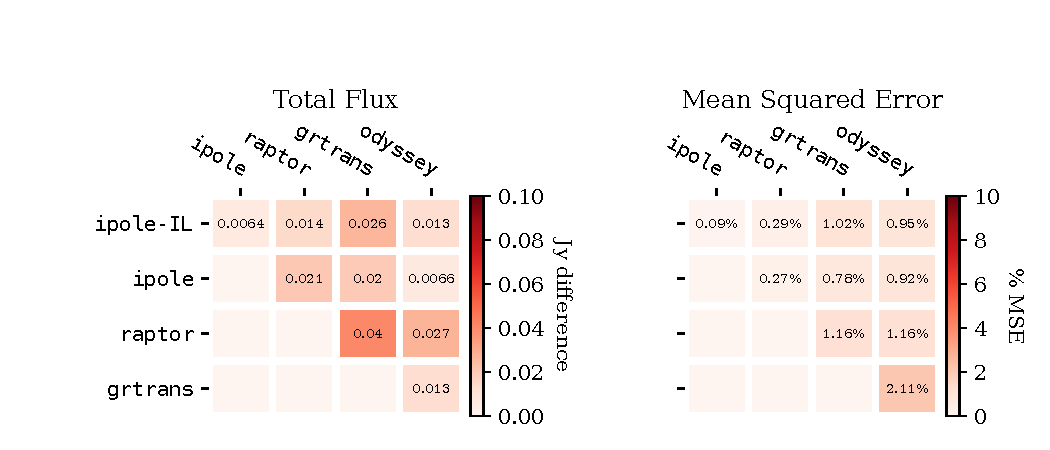
\includegraphics[width=0.95\textwidth]{figures/grmhd_hi_IntegratedUnpolarizeds_plot.pdf}
  \caption{Tables comparing the outputs from several radiative transfer codes used within the EHT for generating images of GRMHD models.  The left table compares total flux between all images (all fluxes were about 0.5\,Jy). The right table compares the Mean Squared Error, described in Section \ref{app:radtrans}, which compares image contents.}
  \label{fig:radtrans_grmhd_comp}
\end{figure*}

Two extensive studies have been undertaken within the EHT Collaboration comparing radiative transfer methods used to evaluate models.  The first, \citep{2020ApJ...897..148G}, evaluated the consistency between general relativistic ray-traced radiative transfer (GRRT) codes when tracing geodesics and when integrating the unpolarized radiative transfer equation.  The second, \citet{Prather_et_al_2022}, evaluates code performance when imaging GRMHD simulation output and when integrating the equations of polarized radiative transfer.

Several EHT radiative transfer codes participated in a comparison exercise, in which each code produced an image of the same GRMHD snapshot file, designed to realistically simulate an image of the black hole \m87 with 230\GHz total flux of 0.5\,Jy.  Figure \ref{fig:radtrans_grmhd_comp} shows tables comparing the total flux of the resulting images, as well as image differences measured by the mean squared error (MSE) between images, defined as
\begin{align}
    \mathrm{MSE}(A, B) &= \frac{\sum_j|A_j-B_j|^2}{\sum_j|A_j|^2}
\end{align}
summed over each image pixel $j$. All images agree to 0.04\,Jy (8\%) in flux, and to a mean squared error of 0.0211, recorded by convention as a percentage 2.11\%.  This level of agreement far exceeds the detector uncertainties in the EHT measurements of \sgra or \m87, rendering the choice of GRRT code irrelevant in producing images for analyses in this paper.

The image field of view (FOV) is another potential concern in evaluating models -- the need for efficiency in generating the millions of images used in this analysis was weighed against any emission which might be missed in images with small FOV. For models which pass size \& other constraints, the FOV is large enough to capture relevant emission, as shown in Figure~\ref{fig:radtrans_fov_study}.

\begin{figure}
  \centering
  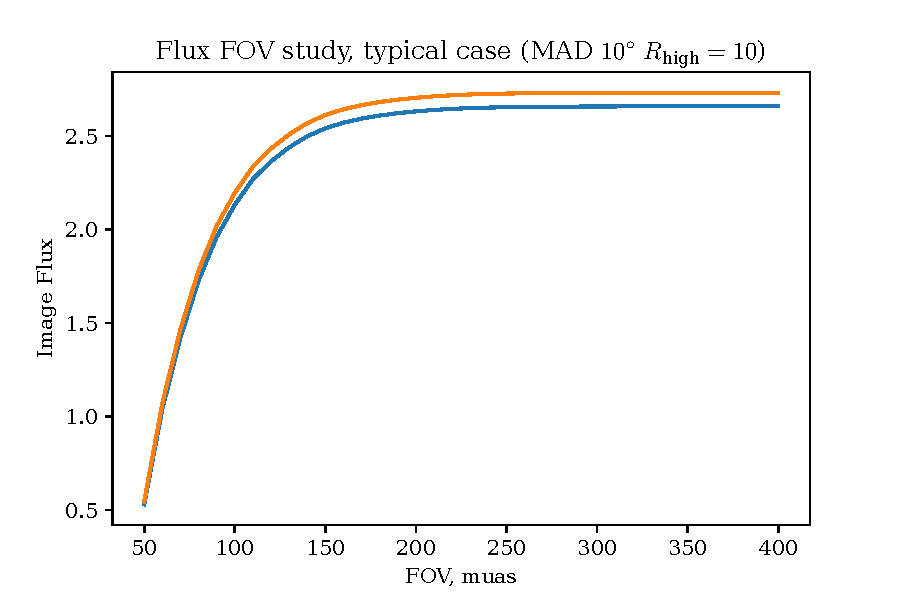
\includegraphics[width=0.45\textwidth]{figures/fov_study.pdf}
  \caption{Flux produced by an image vs the camera field of view. The nominal FOV of $200\uas$ is enough to capture 99\% of emission from this model.\monika{add what are the two different lines: what does the color codes}}
  \label{fig:radtrans_fov_study}
\end{figure}

%==============================================================================
\subsection{GRMHD Simulations Consistency and Convergence}\label{app:resolution_study}

% note: passfail tables are consistently, e.g., tab:illinoisPF or tab:VKhamrPF

%commented out cause there is only ine subsubsection here
%\subsubsection{Comparison of \kharma and \bhac thermal models}

As evident in Table~\ref{tab:GRMHDmodels} the thermal models have been calculated for an identical parameter space from two different codes, namely \kharma and \bhac for the GRMHD simulations and \ipole and \bhoss codes for the GRRT calculations. This allows us for the first time to perform an in depth comparison between the different numerical methods used in this work in addition to the EHTC code comparison projects \citep{2019ApJS..243...26P,2020ApJ...897..148G}.

\begin{figure*}
  \centering
  \includegraphics[width=0.8\textwidth]{./figures/BHAC_iharm_correlation2}
  \caption{Correlation between \bhac and \kharma models for 9 model constraints.  The horizontal axis is the constraint value from \bhac/\bhoss, and the vertical axis shows the constraint value from \kharma/\ipole.  Each point corresponds to a single model, with the width of the distribution shown by the error bars.  See text for details.}
  \label{fig:modelcorrelation}
\end{figure*}

In Figure \ref{fig:modelcorrelation} we show the correlation between the thermal \kharma and \bhac models for constraints where we have predictions from both models.

The top row shows from left to right the 230\,GHz flux density, the 230\GHz modulation index, MI, computed for a time window of 3 hours, and the 230\GHz image size obtained from image moments. Since we normalise the 230\GHz images to an average flux of 2.4\,Jy within a time window of 5000\,M (corresponds to 28.5 h for \sgra a mass of $4.14\times 10^6\,\msun$), the scatter around this values is small. The deviation from an ideal correlation reflects the precision and number of GRMHD snapshots included during normalization procedure.

The correlation in the 3\,hour modulation index $\mi{3}$ spreads over $\Delta \mi{3}=0.75$ which serves as a measure of intra-code ( e.g., MAD vs. SANE accretion) and inter-code (\bhac vs. \kharma) differences. Despite these differences the models show a strong correlation throughout the investigated models and parameter space.

We found a strong correlation between models and codes for the image size computed from image moments, i.e. second moments analysis.

\cfg{This may change if we recompute the major axis, etc., for the IL 86\GHz large fov images}
The middle row presents the correlation plots for the 86\GHz flux density (left), the 86\,GHz image size using second moments (middle) and the NIR flux (right). The 86\GHz flux and 86\GHz image size exhibit a shift toward larger values for the \bhac models. This difference can be explained by the larger field of view used for the \bhac models at 86\GHz during the radiative transfer calculations. Thus, more extended structure and therefore a larger total flux is included in the \bhac models. This affects mainly models with large inclinations $i\geq70^\circ$ and jet dominated emission models ($\rm{R}_{\rm high}\geq 40$).

The NIR fluxes show a tight correlation over four orders of magnitude and systematically larger flux for the \bhac models for low NIR fluxes ($\log_{10}(NIR) < -7$). These fluxes are far below the NIR constraints of $\sim 1\,\mathrm{mJy}$, and therefore they do not affect the passing or failing of the models. In the thermal models the NIR flux is generated from the tail of the electron distribution function and is thus very sensitive to the electron temperature. Small differences in the distribution and value of the electron temperature between the two codes explain the observed de-correlation at very low NIR flux.

The correlation between models for the m-ring parameters is presented in the third row of Figure~\ref{fig:modelcorrelation}. The correlation of the diameter of the m-ring is plotted in the left panel. The spread covers nearly the same extent as the 230\GHz image size (top row, right panel) however the scatter in the correlation is larger.  The same is true for the width of the m-ring (middle panel in the last row of Figure~\ref{fig:modelcorrelation}). Compared to the diameter and width of the m-ring, the asymmetry of the m-ring is less correlated (right panel). Notice that horizontal and vertical limits in the asymmetries occur since the parameter hits the boundary of the allowed range.

The smaller correlation of the m-ring parameters as compared to the other parameters presented in Figure~\ref{fig:modelcorrelation} is a consequence of the noisy nature of the m-ring fits.  Still, the distributions are quite symmetric under reflection across the diagonal, so the models are at least not biased with respect to each other.  Notice also that these plots do not capture all the information that is contained in the distribution of m-ring parameters, just the central value.

We are somewhat surprised by the strength of the correlations seen in Figure~\ref{fig:modelcorrelation}.  The range of each constraint is significantly larger than the width of the correlation, so the variations between models are real, detectable, and reproducible with independent codes.  The question of the origin of the systematic offsets between models for some constraints (for example, in the NIR) is interesting but beyond the scope of this paper.

%\monika{Dec11:  in this subsection we only show details. if hamr scoring is consistent with kharma/bhac then this should be reported in the main text, not appendix; commenting this out due to lower statistics in hamr models}

% \subsubsection{Comparison of \hamr and \kharma thermal models}

% %\note{Doosoo, Koushik to write here about HAMR thermal models.}
% Along the \kharma/\ipole and \bhac/\bhoss models, we produced a set of thermal models out to $35,000\tg$ using the GRMHD code \hamr and the GRRT code \bhoss (see Table~\ref{tab:GRMHDmodels}). These models consider a gas adiabatic index of $\Gamma_{\rm ad}=5/3$ for the SANE models and $\Gamma_{\rm ad}=13/9$ for the MAD models (Table~\ref{tab:radiativemodels}), allowing us to understand how sensitive the images are to the GRMHD fluid properties, in addition to code numerics.

% We report that overall, the \hamr/\bhoss thermal eDF images perform similarly to the \kharma/\ipole and \bhac/\bhoss models. \kc{needs verification from Michi}

% \kc{is the plan to do H-AMR and KHARMA correlations similar to figure 18?}

\clearpage

\section{Variability Checks}\label{app:variability}

\note{David, Vedant to provide first draft}

The discussion section lists several possible causes for the apparently high variability of the models in comparison to the data.

Here we discuss and dismiss some of these possibilities.

%==============================================================================
1. GRMHD resolution.

discussion of varying resolution [Ben to spelunk to find a 448 down set of images]

Discussion of high resolution HAMR model.

mapping between 230 GHz variability and accretion rate variability

%==============================================================================
2. Image resolution.

%==============================================================================
3. Model duration is not sufficiently long.

KORAL model analysis.

%==============================================================================
4. $\sigma_{cut}$ is overproducing variability.

%==============================================================================
5. Initial conditions are not a good model.

Comparison of Monika model initial conditions

%==============================================================================
6. Cooling filters the light curve. [Ben]

Discussion of model with $\Theta_{e,max}(r, \tau_{cool})$

%==============================================================================
%7. Electron distribution function model is inadequate.

%a.  Discussion of models with varying electron heating models.  Discussion of Jason's eheating models.   Forward reference to Diaz et al.  [Vedant]

%b. Discussion of models with $\Rl = 10$. [Vedant]

\subsection{Effects of self-consistent electron heating models}

The \textit{thermal} models considered in \textcolor{magenta}{ref. models section} assign a local electron temperature as a post-processing step based on local magnetic field strength, parameterized by plasma $\beta$ (\textcolor{magenta}{ref. Rhigh and critical beta equations}).

\citealt{10.1093/mnras/stv2084} provided a formulation to self-consistently model electron thermodynamics during the fluid evolution. Numerical dissipation at grid scale sources entropy generation and is used to heat the electrons based on a microphysical, sub-grid heating prescription. Local fluid and electromagnetic variables are used to compute the electron entropy which along with the ideal gas equation of state, can be converted into a temperature ($\Theta_{e}$). This approach allows computing the electron temperature at each timestep of the simulation, and not during post-processing, as it is done in the $R_{high}$ and Critical-$\beta$ prescriptions.

We consider three sub-grid heating models that prescribe the partition of dissipated energy into electrons and ions. \citealt{2010MNRAS.409L.104H} computed the ratio of ion-to-electron heating due to dissipation of Alfv\'enic turbulent cascade, while \citealt{10.1093/mnras/stx2530} and \citealt{Rowan_2017} considered magnetic reconnection as the source of energy dissipation at sub-grid scales. These studies provide an approximate fitting formula for the ion-to-electron heating rate ($Q_{i}/Q_{e}$) based on local ion-to-electron temperature ratio ($T_{i}/T_{e}$) and local magnetic field strength -- parameterized by $\sigma$ or plasma $\beta$.

The GRMHD simulations considered here are a subset of the simulations analyzed in \citealt{2020MNRAS.494.4168D}. These include MAD and SANE accretion flows at spins, $a_{*}=0,+1/2,+15/16$. We compute the 3 hour modulation index $M_{3}$, over the time interval (5k-10k)$GM/c^{3}$. The average $M_{3}$ values are comparable to similar $R_{high}$ models, with SANE reconnection models exhibiting a reduced variability as compared to the corresponding turbulent heating models. However, the average $M_{3}$ for all the models is greater than the $M_{3}$ measured from the ALMA lightcurve on three days.

%==============================================================================
\subsection{Effect of $\Rl$}

The $R_{high}$ prescription (Equation \textcolor{magenta}{ref. Rhigh equation}) has three free parameters: $R_{high}$, $R_{low}$ and $\beta_{crit}$. During post-processing, the $R_{high}$ parameter is generally varied while $R_{low}$ and $\beta_{crit}$ is set to unity. In this section we investigate the effect of varying $R_{low}$ on the 3 hour modulation index, $M_{3}$.

Paticle-in-cell (PIC) simulations modelling turbulent dissipation or dissipation associated with magnetic reconnection suggest preferential heating of the electrons in regions of low plasma $\beta$ (\citealt{2010MNRAS.409L.104H, Rowan_2017, 10.1093/mnras/stx2530, Rowan_2019, Kawazura771, PhysRevX.10.041050, kawazura2021energy}). The $R_{low}$ parameter dictates the electron temperature in these regions, that is, in the funnel. Figure \ref{fig:rlow_comparison} shows the effect of $R_{low}$ on image morphology.

\begin{figure*}
\centering
\includegraphics[width=0.95\textwidth]{figures/rlow_comparison_rhigh160.png}
\caption{Comparison of images for the same fluid snapshot with varying $\Rl$. The density scale $\mathcal{M}$, and FOV were increased to accentuate the differences between the images. The total emission in the funnel is an inverse function of $\Rl$.}
\label{fig:rlow_comparison}
\end{figure*}

For systems with low accretion rates, $\Dot{M}\ll\Dot{M}_{Edd}$, such as SgrA$^{*}$ (\textcolor{magenta}{include refs for SgrA accretion rate and ref. to section on accretion rates}), radiative processes can be neglected during fluid evolution (\citealt{2012MNRAS.426.1928D, 10.1093/mnras/stw3116, Ryan_2017}) and the plasma can be considered Coulomb collisionless (\citealt{Mahadevan_1997, 10.1093/mnras/stw3116, Ryan_2017}). However, the uncertainties with electron heating and advection, and a limited understanding of the funnel warrant a discussion of cooler electrons in regions of high magnetization, and in particular, its effect on submm lightcurve variability. We vary $R_{low}$ for a select set of the best bet Illinois/Thermal models and plot the distribution of the 3 hour modulation index $M_{3}$ in Figure \ref{fig:mi_rlow}.

\begin{figure*}
\centering
\includegraphics[width=0.95\textwidth]{figures/mi_rlow_select_models.pdf}
\caption{Modulation index computed over 3 hour intervals $M_{3}$ for a subset of the Illinois/Thermal models that pass all the constraints. For this analysis, we considered the (25k-30k)$GM/c^{3}$ time interval.}
\label{fig:mi_rlow}
\end{figure*}

Although the minimum value of the distribution decreases when $R_{low}$ is increased, there is no clear trend for the mean of the distribution. In addition, the average $M_{3}$ still does not match observational values.

%==============================================================================
8. The flow is actually made of helium. [George]

brief discussion, forward reference to Wong+.

%==============================================================================
%9. $\gamma = 5/3$ rather than $4/3$.   [Vedant]  When $\gamma = 4/3$ the compression ratio across the shock is larger.

\subsection{Effect of fluid adiabatic index, $\Gamma_{\lowercase{ad}}$}

We expect the ions and electrons in in hot accretion flows to be thermally decoupled and the resulting plasma to be two-temperature (\citealt{1976ApJ...204..187S, Quataert_1998, 10.1093/mnras/stw3116, Ryan_2018}). The electrons in such flows are relativistic and can be modelled as a fluid with an adiabatic index $\Gamma_{e}=4/3$, while the ions are nonrelativistic and possess an adiabatic index, $\Gamma_{i}=5/3$.

The adiabatic index of the fluid assumes a value between $\Gamma_{e}$ and $\Gamma_{i}$ dictated by the thermodynamics of the ions and electrons (cf. Figure 4 in \citealt{10.1093/mnras/stw3116}). Since we do not model electron thermodynamics and ignore radiative effects during our fluid simulations, we consider a constant value $\Gamma_{ad}$, and set it to 4/3 for the \textit{standard} set of simulations, ie. $\Gamma_{ad}=\Gamma_{e}$. While this may be the case in the funnel, where the electrons are the hottest and highly relativistic; the fluid adiabatic index value away from the poles can be higher than the relativistic value.

We look at the interplay between fluid adiabatic index and lightcurve variability by evaluating $M_{3}$ for thermal, GRMHD models with a higher fluid adiabatic index. This includes MAD models with $\Gamma_{ad}=13/9$ (\textcolor{magenta}{ref. section on KORAL models}; \citealt{2021arXiv210812380N}) and SANE models with $\Gamma_{ad}=5/3$. The models exhibit lightcurve variability similar to the \textit{standard} library and have an average $M_{3}$ that is greater than the value obtained from the ALMA lightcurve.

\clearpage

%==============================================================================
% Ensure that papers are listed in the references
\nocite{M87PaperI}
\nocite{M87PaperII}
\nocite{M87PaperIII}
\nocite{M87PaperIV}
\nocite{M87PaperV}
\nocite{M87PaperVI}
\nocite{M87PaperVII}
\nocite{M87PaperVIII}
\nocite{PaperI}
\nocite{PaperII}
\nocite{PaperIII}
\nocite{PaperIV}
\nocite{PaperV}
\nocite{PaperVI}

\bibliographystyle{yahapj}
\bibliography{main,EHTCPapers}

%==============================================================================
\end{document}
